%------------------------------------------------------------------------------------------
% Meta-commands for the TeXworks editor
%
% !TeX root = ../Esercizi_MS.tex
% !TEX encoding = UTF-8
% !TEX program = pdflatex
%
%============================================================================================
%

\begin{comment}

\setcounter{chapter}{0}
\chapter{Nozioni introduttive}

%===============================================================================================
%--BEGIN-EXERCISE:equivalent_airspeed_basic_1
%
\def\mySpanWingMT{10.600000}
\def\mySpanWingIMT{6.360000}
\def\mySpanWingIIMT{4.240000}
\def\myChordRootWingMT{1.440000}
\def\myChordRootWingIMT{1.440000}
\def\myChordRootWingIIMT{1.440000}
\def\myChordTipWingMT{0.860000}
\def\myChordTipWingIMT{1.440000}
\def\myChordTipWingIIMT{0.860000}
\def\mySweepLEWingIIDEG{0.000000}
\def\myCoeffAChordWingI{0.000000}
\def\myCoeffBChordWingIMT{1.440000}
\def\myCoeffAChordWingII{-0.273585}
\def\myCoeffBChordWingIIMT{1.440000}
\def\myAlphaZeroLiftRootWingIDEG{-2.500000}
\def\myAlphaZeroLiftTipWingIDEG{-2.500000}
\def\myAlphaZeroLiftRootWingIRAD{-0.043633}
\def\myAlphaZeroLiftTipWingIRAD{-0.043633}
\def\myAlphaZeroLiftRootWingIIDEG{-2.500000}
\def\myAlphaZeroLiftTipWingIIDEG{-1.000000}
\def\myAlphaZeroLiftRootWingIIRAD{-0.043633}
\def\myAlphaZeroLiftTipWingIIRAD{-0.017453}
\def\myTaperRatioWingI{1.000000}
\def\myTaperRatioWingII{0.597222}
\def\myTwistWingIDEG{0.000000}
\def\myTwistWingIRAD{0.000000}
\def\myTwistWingIIDEG{-3.000000}
\def\myTwistWingIIRAD{-0.052360}
\def\myAreaWingIMTsquared{9.158400}
\def\myAreaWingIIMTsquared{4.876000}
\def\myAreaWingMTsquared{14.034400}
\def\myCoeffAAeroTwistWingIRADMT{0.000000}
\def\myCoeffBAeroTwistWingIRAD{-0.043633}
\def\myCoeffAAeroTwistWingIIRADMT{0.012349}
\def\myCoeffBAeroTwistWingIIRAD{-0.043633}
\def\myCoeffATwistWingIRADMT{0.000000}
\def\myCoeffATwistWingIIRADMT{-0.024698}
\def\myCoeffBTwistWingIRAD{0.000000}
\def\myCoeffBTwistWingIIRAD{0.000000}
\def\myAlphaZeroLiftWingIRAD{-0.028653}
\def\myAlphaZeroLiftWingIDEG{-1.641680}
\def\myAlphaZeroLiftWingIIRAD{0.008329}
\def\myAlphaZeroLiftWingIIDEG{0.477233}
\def\myAlphaZeroLiftWingRAD{-0.020323}
\def\myAlphaZeroLiftWingDEG{-1.164447}

%
\begin{myExampleX}{Velocità vera e velocità equivalente}{\ding{46}}% \ \Keyboard\ %
\label{example:Equivalent:Airspeed:Basic:A}
%
\noindent
Una velocità equivalente 
$V_\mathrm{e}
 =\SI[round-precision=0]{\myFlightSpeedEASKMH}{km/h}
 =\SI[round-precision=1]{\myFlightSpeedEASMTSec}{m/s}$
corrisponde a un determinato valore della velocità vera $V\equiv V_\mathrm{t}$ in quota.

All'altitudine $h=\SI[round-precision=0]{\myAltitudeMT}{m}$ si ha
una densità dell'aria $\rho=\SI[round-precision=3]{\myAirDensityKGMTcubed}{kg/m^3}$
e la velocità vera di volo è
\[
V = 
  \frac{ V_\text{e} }{ \sqrt{\dfrac{\rho}{\rho_\mathrm{SL}}} }
  = 
  \frac{
    \SI[round-precision=1]{\myFlightSpeedEASMTSec}{m/s}
  }{
    \sqrt{
      \dfrac{
        \SI[round-precision=3]{\myAirDensityKGMTcubed}{kg/m^3}
      }{
        \SI[round-precision=3]{\myISAAirDensitySeaLevelKGMTcubed}{kg/m^3}
      }
    }
  }
= 
  \mathunderline{mydarkblue}{ \SI[round-precision=1]{\myFlightSpeedMTSec}{\meter/\second} }
  = \mathunderline{mydarkblue}{ \SI[round-precision=1]{\myFlightSpeedKMH}{\kilo\meter/\hour} }
\]
che come si vede ha un valore più elevato della $V_\mathrm{e}$ corrispondente.

\end{myExampleX}
%
%--END-EXERCISE:equivalent_airspeed_basic_1
%===============================================================================================

%===============================================================================================
%--BEGIN-EXERCISE:velocity_components_basic_1
%
\def\mySpanWingMT{10.600000}
\def\mySpanWingIMT{6.360000}
\def\mySpanWingIIMT{4.240000}
\def\myChordRootWingMT{1.440000}
\def\myChordRootWingIMT{1.440000}
\def\myChordRootWingIIMT{1.440000}
\def\myChordTipWingMT{0.860000}
\def\myChordTipWingIMT{1.440000}
\def\myChordTipWingIIMT{0.860000}
\def\mySweepLEWingIIDEG{0.000000}
\def\myCoeffAChordWingI{0.000000}
\def\myCoeffBChordWingIMT{1.440000}
\def\myCoeffAChordWingII{-0.273585}
\def\myCoeffBChordWingIIMT{1.440000}
\def\myAlphaZeroLiftRootWingIDEG{-2.500000}
\def\myAlphaZeroLiftTipWingIDEG{-2.500000}
\def\myAlphaZeroLiftRootWingIRAD{-0.043633}
\def\myAlphaZeroLiftTipWingIRAD{-0.043633}
\def\myAlphaZeroLiftRootWingIIDEG{-2.500000}
\def\myAlphaZeroLiftTipWingIIDEG{-1.000000}
\def\myAlphaZeroLiftRootWingIIRAD{-0.043633}
\def\myAlphaZeroLiftTipWingIIRAD{-0.017453}
\def\myTaperRatioWingI{1.000000}
\def\myTaperRatioWingII{0.597222}
\def\myTwistWingIDEG{0.000000}
\def\myTwistWingIRAD{0.000000}
\def\myTwistWingIIDEG{-3.000000}
\def\myTwistWingIIRAD{-0.052360}
\def\myAreaWingIMTsquared{9.158400}
\def\myAreaWingIIMTsquared{4.876000}
\def\myAreaWingMTsquared{14.034400}
\def\myCoeffAAeroTwistWingIRADMT{0.000000}
\def\myCoeffBAeroTwistWingIRAD{-0.043633}
\def\myCoeffAAeroTwistWingIIRADMT{0.012349}
\def\myCoeffBAeroTwistWingIIRAD{-0.043633}
\def\myCoeffATwistWingIRADMT{0.000000}
\def\myCoeffATwistWingIIRADMT{-0.024698}
\def\myCoeffBTwistWingIRAD{0.000000}
\def\myCoeffBTwistWingIIRAD{0.000000}
\def\myAlphaZeroLiftWingIRAD{-0.028653}
\def\myAlphaZeroLiftWingIDEG{-1.641680}
\def\myAlphaZeroLiftWingIIRAD{0.008329}
\def\myAlphaZeroLiftWingIIDEG{0.477233}
\def\myAlphaZeroLiftWingRAD{-0.020323}
\def\myAlphaZeroLiftWingDEG{-1.164447}

%
\begin{myExampleX}{Angoli aerodinamici e componenti di Velocità}{\ding{46}}% \ \Keyboard\ %
\label{example:Velocity:Components:Basic:A}
%
\noindent
Un velivolo procede alla velocità 
$V\equiv |\vec{V}|=\SI[round-precision=0]{\myFlightSpeedKTS}{\knots}
  =\SI[round-precision=1]{\myFlightSpeedKMH}{km/h}=\SI[round-precision=2]{\myFlightSpeedMTSec}{m/s}$,
con un angolo d'attacco 
$\alpha_\Body=\SI[round-precision=0]{\myAngleOfAttackBodyDEG}{deg}
  =\SI[round-precision=4]{\myAngleOfAttackBodyRAD}{\radian}$
e un angolo di derapata
$\beta=\SI[round-precision=0]{\myAngleOfSideslipBodyDEG}{deg}
  =\SI[round-precision=4]{\myAngleOfSideslipBodyRAD}{\radian}$.

Le componenti di velocità risultano essere
\[
\begin{split}
u = V \cos\beta \cos\alpha_\Body
  & {}= \SI[round-precision=2]{\myFlightSpeedMTSec}{m/s}
    \cdot \cos\big( \SI[round-precision=4]{\myAngleOfSideslipBodyRAD}{\radian} \big)
    \cdot \cos\big( \SI[round-precision=4]{\myAngleOfAttackBodyRAD}{\radian} \big)
\\
  & {}= \mathunderline{mydarkblue}{ \SI[round-precision=2]{\myUBodyMTSec}{\meter/\second} }
  = \mathunderline{mydarkblue}{ \SI[round-precision=1]{\myUBodyKMH}{\kilo\meter/\hour} }
\end{split}
\]

\[
\begin{split}
v = V \sin\beta
  & {}= \SI[round-precision=2]{\myFlightSpeedMTSec}{m/s}
    \cdot \sin\big( \SI[round-precision=4]{\myAngleOfSideslipBodyRAD}{\radian} \big)
\\
  & {}= \mathunderline{mydarkblue}{ \SI[round-precision=2]{\myVBodyMTSec}{\meter/\second} }
  = \mathunderline{mydarkblue}{ \SI[round-precision=1]{\myVBodyKMH}{\kilo\meter/\hour} }
\end{split}
\]

\[
\begin{split}
w = V \cos\beta \sin\alpha_\Body
  & {}= \SI[round-precision=2]{\myFlightSpeedMTSec}{m/s}
    \cdot \cos\big( \SI[round-precision=4]{\myAngleOfSideslipBodyRAD}{\radian} \big)
    \cdot \sin\big( \SI[round-precision=4]{\myAngleOfAttackBodyRAD}{\radian} \big)
\\
  & {}= \mathunderline{mydarkblue}{ \SI[round-precision=2]{\myWBodyMTSec}{\meter/\second} }
  = \mathunderline{mydarkblue}{ \SI[round-precision=1]{\myWBodyKMH}{\kilo\meter/\hour} }
\end{split}
\]

La componente $u$ ha un valore molto prossimo a quello della velocità lungo la traiettoria 
$|\vec{V}|$. La componente $v$ rappresenta l'intensità della corrente di \emph{cross-flow},
la quale determina l'insorgere di componenti aerodinamiche non nulle di forza laterale, 
di momento di rollio e di momento d'imbardata.
La componente $w$ è determinata dall'inclinazione della fusoliera rispetto alla corrente
asintotica ed è collegata direttamente alla portanza generata.

\end{myExampleX}
%
%--END-EXERCISE:velocity_components_basic_1
%===============================================================================================

%===============================================================================================
%--BEGIN-EXERCISE:ISA_atmosphere_basic_1
%
\def\mySpanWingMT{10.600000}
\def\mySpanWingIMT{6.360000}
\def\mySpanWingIIMT{4.240000}
\def\myChordRootWingMT{1.440000}
\def\myChordRootWingIMT{1.440000}
\def\myChordRootWingIIMT{1.440000}
\def\myChordTipWingMT{0.860000}
\def\myChordTipWingIMT{1.440000}
\def\myChordTipWingIIMT{0.860000}
\def\mySweepLEWingIIDEG{0.000000}
\def\myCoeffAChordWingI{0.000000}
\def\myCoeffBChordWingIMT{1.440000}
\def\myCoeffAChordWingII{-0.273585}
\def\myCoeffBChordWingIIMT{1.440000}
\def\myAlphaZeroLiftRootWingIDEG{-2.500000}
\def\myAlphaZeroLiftTipWingIDEG{-2.500000}
\def\myAlphaZeroLiftRootWingIRAD{-0.043633}
\def\myAlphaZeroLiftTipWingIRAD{-0.043633}
\def\myAlphaZeroLiftRootWingIIDEG{-2.500000}
\def\myAlphaZeroLiftTipWingIIDEG{-1.000000}
\def\myAlphaZeroLiftRootWingIIRAD{-0.043633}
\def\myAlphaZeroLiftTipWingIIRAD{-0.017453}
\def\myTaperRatioWingI{1.000000}
\def\myTaperRatioWingII{0.597222}
\def\myTwistWingIDEG{0.000000}
\def\myTwistWingIRAD{0.000000}
\def\myTwistWingIIDEG{-3.000000}
\def\myTwistWingIIRAD{-0.052360}
\def\myAreaWingIMTsquared{9.158400}
\def\myAreaWingIIMTsquared{4.876000}
\def\myAreaWingMTsquared{14.034400}
\def\myCoeffAAeroTwistWingIRADMT{0.000000}
\def\myCoeffBAeroTwistWingIRAD{-0.043633}
\def\myCoeffAAeroTwistWingIIRADMT{0.012349}
\def\myCoeffBAeroTwistWingIIRAD{-0.043633}
\def\myCoeffATwistWingIRADMT{0.000000}
\def\myCoeffATwistWingIIRADMT{-0.024698}
\def\myCoeffBTwistWingIRAD{0.000000}
\def\myCoeffBTwistWingIIRAD{0.000000}
\def\myAlphaZeroLiftWingIRAD{-0.028653}
\def\myAlphaZeroLiftWingIDEG{-1.641680}
\def\myAlphaZeroLiftWingIIRAD{0.008329}
\def\myAlphaZeroLiftWingIIDEG{0.477233}
\def\myAlphaZeroLiftWingRAD{-0.020323}
\def\myAlphaZeroLiftWingDEG{-1.164447}

%
\begin{myExampleX}{Caratteristiche dell'aria in quota}{\ding{46}}% \ \Keyboard\ %
\label{example:Atmosphere:Basic:A}
%
\noindent
Si vogliono calcolare le caratteristiche dell'aria tipo secondo il modello ISA ad un'ipotetica quota di volo
$h=\SI[round-precision=0]{\myAltitudeMT}{\meter}$. 
Per un numero di Mach di volo $\Mach=\SI[round-precision=2]{\myMach}{}$
si vuole poi determinare la velocità vera e il numero di Reynolds di volo per unità di lunghezza 
$\Reynolds/l_\mathrm{ref}$.

La quota assegnata è al di sotto degli \SI[round-precision=0]{11}{\kilo\meter} dunque
nel modello ISA va assunto un gradiente di temperatura
$\mathit{LR}=\SI[round-precision=4]{\myISALapseRateKMT}{\kelvin/\meter}$.
Pertanto la temperatura in quota è
\[
T = T_{\text{SL}} - \mathit{LR} \, h  
  = \SI[round-precision=2]{\myISAAirTemperatureSeaLevelK}{\kelvin}
    + \big( \SI[round-precision=4]{\myISALapseRateKMT}{\kelvin/\meter} \big)
      \cdot \SI[round-precision=0]{\myAltitudeMT}{\meter}
  = \mathunderline{mydarkblue}{ \SI[round-precision=1]{\myAirTemperatureK}{\kelvin} }
\]
a cui corrisponde una velocità del suono
\[
a = \sqrt{\thinspace \gamma_\text{air} R_\text{air} T\thinspace}
  = \sqrt{\thinspace 
      \SI[round-precision=1]{\myISAAirAdiabaticIndex}{} 
      \cdot \SI[round-precision=2]{\myISAAirGasConstNMTKGK}{\newton\,\metre\,\kilogram^{-1}\,\kelvin^{-1}}
      \cdot \SI[round-precision=1]{\myAirTemperatureK}{\kelvin}
    \thinspace}
  = \mathunderline{mydarkblue}{ \SI[round-precision=2]{\myAirSoundSpeedMTSec}{\meter/\second} }
\]
Per i valori assegnati del numero di Mach di volo e della quota si così ha una velocità di volo
\[
V = a \, \Mach
  =  \SI[round-precision=2]{\myAirSoundSpeedMTSec}{\meter/\second} \cdot \SI[round-precision=2]{\myMach}{}
  = \mathunderline{mydarkblue}{ \SI[round-precision=2]{\myFlightSpeedMTSec}{\meter/\second} }
  = \mathunderline{mydarkblue}{ \SI[round-precision=1]{\myFlightSpeedKMH}{\kilo\meter/\hour} }
\]

%--------------------------------------------
%\pgfkeys{
%   /pgf/fpu=true,
%   /pgf/fpu/output format=fixed,% sci
%}
%\pgfmathparse{1+1}
%\SI[round-precision=3]{\pgfmathresult}{\meter}
%--------------------------------------------
%
La densità relativa vale
\[
\begin{split}
\sigma = \frac{\rho}{\rho_\mathrm{SL}}
  & {} = 
    \Bigg(
      \frac{T}{T_\mathrm{SL}}
    \Bigg)^{-\left(\dfrac{g}{\mathit{LR}\cdot R_\mathrm{air}}+1\rule[-1.1em]{0pt}{2.4em}\right)}
  % ^{\num[round-precision=3]{4.257}}\;,
\\
  & {} =
    \Bigg(
      \frac{ 
        \SI[round-precision=1]{\myAirTemperatureK}{\kelvin} 
    }{
      \SI[round-precision=2]{\myISAAirTemperatureSeaLevelK}{\kelvin}
    }
    \Bigg)^{-\left(
      \dfrac{
        \SI[round-precision=2]{9.81}{\meter/\second^2}
      }{
        \SI[round-precision=4]{\myISALapseRateKMT}{\kelvin/\meter}
          \cdot \SI[round-precision=2]{\myISAAirGasConstNMTKGK}{\newton\,\metre\,\kilogram^{-1}\,\kelvin^{-1}}
      }
      + 1
      %\rule[-1.1em]{0pt}{2.4em}% --> SPACER
    \right)}
    = \mathunderline{mydarkblue}{ \SI[round-precision=3]{\myAirDensityRatio}{} }
\end{split}
\]
quindi la densità dell'aria alla quota di volo è
\[
\rho = \rho_\mathrm{SL} \, \sigma =
    \SI[round-precision=3]{\myISAAirDensitySeaLevelKGMTcubed}{\kilogram\,\meter^{-3}}
      \cdot \SI[round-precision=3]{\myAirDensityRatio}{} 
    = \mathunderline{mydarkblue}{ \SI[round-precision=3]{\myAirDensityKGMTcubed}{\kilogram\,\meter^{-3}} }
\]
Questo valore e il valore della velocità di volo permettono il calcolo della
pressione dinamica di volo
\[
\bar{q} = \frac{1}{2} \rho V^2 =
  \num{0.5} \cdot \SI[round-precision=3]{\myAirDensityKGMTcubed}{\kilogram\,\meter^{-3}}
    (\SI[round-precision=2]{\myFlightSpeedMTSec}{\meter/\second}\big)^2
  = \mathunderline{mydarkblue}{ \SI[round-precision=2]{\myFlightQbarPA}{\newton\,\meter^{-2}} }
  = \mathunderline{mydarkblue}{ \SI[round-precision=3]{\myFlightQbarBAR}{ bar } }
\]

Infine, la viscosità dinamica dell'aria alla quota assegnata è
\[
\begin{split}
\mu 
  & ={}
    \num[round-precision=3]{1.458}\cdot 10^{-6}\,\SI{}{\kilogram.\Big(\meter.\second.\SQRT{\kelvin}\Bigr)^{\!-1}} \cdot
    \frac{ T^{3/2} }
    { T + \SI[round-precision=1]{110.4}{\kelvin} }
\\[0.5em]
  & ={}
    \num[round-precision=3]{1.458}\cdot 10^{-6}\,\SI{}{\kilogram.\Big(\meter.\second.\SQRT{\kelvin}\Bigr)^{\!-1}} \cdot
    \frac{ \big(\SI[round-precision=1]{\myAirTemperatureK}{\kelvin}\big)^{3/2} }
    { \SI[round-precision=1]{\myAirTemperatureK}{\kelvin} + \SI[round-precision=1]{110.4}{\kelvin} }
\\[0.5em]
  & ={} \mathunderline{mydarkblue}{ \SI[round-precision=3]{\myAirDynamicViscosiyMTSecKG}{ \kilogram\,(\meter\,\second)^{-1} } }
\end{split}
\]
a cui corrisponde un numero di Reynolds per unità di lunghezza
\[
\begin{split}
\frac{\Reynolds}{l_\mathrm{ref}} = \frac{\rho V}{\mu}
  & ={}
    \frac{
      \SI[round-precision=3]{\myAirDensityKGMTcubed}{\kilogram\,\meter^{-3}}
      \cdot \SI[round-precision=2]{\myFlightSpeedMTSec}{\meter/\second}
    }{
      \SI[round-precision=3]{\myAirDynamicViscosiyMTSecKG}{ \kilogram\,(\meter\,\second)^{-1} }
    }
    = \SI[round-precision=3,scientific-notation=true]{\myReynoldsPerUnitLengthMT}{ \meter^{-1} }
\end{split}
\]
\end{myExampleX}
%
%--END-EXERCISE:ISA_atmosphere_basic_1
%===============================================================================================

%===============================================================================================
%--BEGIN-EXERCISE:ES:ISA_atmosphere_basic_2
%
\begin{myExerciseX}{Caratteristiche dell'aria in quota}{\ding{46}}% \ \Keyboard\ %
\label{exercise:Atmosphere:Basic:A}
%
\noindent
Sulla base dell'esempio~\ref{example:Atmosphere:Basic:A} calcolare il numero di Mach
di volo alla quota $h=\SI[round-precision=0]{9000}{\meter}$ per velocità $V$ pari, rispettivamente,
a 
\SI[round-precision=0]{800}{\kilo\meter/\hour},
\SI[round-precision=0]{700}{\kilo\meter/\hour} e
\SI[round-precision=0]{600}{\kilo\meter/\hour}.

Per una lunghezza di riferimento $l_\mathrm{ref}=\SI[round-precision=1]{5.0}{\meter}$
calcolare anche i numeri di Reynolds di volo corrispondenti.
\end{myExerciseX}
%
%--END-EXERCISE:ES:ISA_atmosphere_basic_2
%===============================================================================================

%###############################################################################################
% #  #  #  #  #  #  #  #  #  #  #  #  #  #  #  #  #  #  #  #  #  #  #  #  #  #  #  #  #  #  #  #
%
%\end{document}
%
% #  #  #  #  #  #  #  #  #  #  #  #  #  #  #  #  #  #  #  #  #  #  #  #  #  #  #  #  #  #  #  #
%###############################################################################################

%###############################################################################################

\setcounter{chapter}{1}
\chapter%
  [Azioni aerodinamiche sul velivolo. Nozioni di base]%
  {Azioni aerodinamiche sul velivolo.\\ Nozioni di base}

%===============================================================================================
%--BEGIN-EXERCISE:aerodynamic_coefficient_basic_1
%
% $ bash ./extract_exercise.sh aerodynamic_coefficient_basic_1 ./exercises/Esercizi_MS_Contents.tex ./contents/RichiamiAerodinamica_NozioniBase.tex
%
%
\input{exercises/aerodynamic_coefficient_basic_1/Output/FLIGHT_TeX_Macros.tex}
%\input{exercises/aerodynamic_coefficient_basic_1/Output/WING_TeX_Macros.tex}
%\input{exercises/aerodynamic_coefficient_basic_1/Output/FUSELAGE_TeX_Macros.tex}
%\input{exercises/aerodynamic_coefficient_basic_1/Output/HTAIL_TeX_Macros.tex}
%\input{exercises/aerodynamic_coefficient_basic_1/Output/VTAIL_TeX_Macros.tex}
\input{exercises/aerodynamic_coefficient_basic_1/Output/LONGITUDINAL_TeX_Macros.tex}
%
\begin{myExampleX}{Coefficienti aerodinamici di un velivolo}{\ding{46}}% \ \Keyboard\ %
\label{example:Aerodynamic:Coefficients:Basic:A}
%
\noindent
In questo esempio numerico si effettua il calcolo di un coefficiente aerodinamico a partire
da una forza e, viceversa, il calcolo di una forza aerodinamica noto il coefficiente.

Un velivolo dalle caratteristiche simili a quelle di un Boeing~777-300ER ha una massa 
$m=\SI[round-precision=0]{\myMassKG}{\kilogram}=\SI[round-precision=0]{\myMassLB}{\lbm}$
(cioè un peso pari a circa l'80\% del peso massimo al decollo, \emph{Maximum Take-Off Weight}, MTOW)
e una superficie alare 
$S=\SI[round-precision=1]{\myAreaWingMTsquared}{\meter^2}=\SI[round-precision=1]{\myAreaWingFTsquared}{\feet^2}$.
Per un volo alla velocità 
$V=\SI[round-precision=2]{\myFlightSpeedKTS}{kts}=\SI[round-precision=1]{\myFlightSpeedKMH}{\kilo\meter/\hour}$,
alla quota 
$h=\SI[round-precision=3]{\myAltitudeMT}{\meter}$,
per la quale 
$\rho=\SI[round-precision=3]{\myAirDensityKGMTcubed}{\kilogram\,\meter^{-3}}$,
%(cfr.~esempio~\ref{example:Atmosphere:Basic:A}),
si ha una pressione dinamica di volo
\[
\begin{split}
\bar{q} = \frac{1}{2} \rho V^2 
  & {}=
  \num{0.5} \cdot \SI[round-precision=3]{\myAirDensityKGMTcubed}{\kilogram\,\meter^{-3}}
    \, (\SI[round-precision=2]{\myFlightSpeedMTSec}{\meter/\second}\big)^2
\\
  & {}=
    \mathunderline{mydarkblue}{ 
      \SI[round-precision=3,scientific-notation=true]{\myDynamicPressurePA}{\newton\,\meter^{-2}} 
    }
    = \mathunderline{mydarkblue}{ 
      \SI[round-precision=3,scientific-notation=true]{\myDynamicPressureBAR}{ bar } 
    }
\end{split}
\]
corrispondente a un numero di Mach $M=\SI[round-precision=2]{\myMachNumber}{}$.

Se si assume un volo equilibrato, in cui la portanza $L$ uguaglia il peso $W=mg$, si ha un coefficiente
di portanza $C_L$ pari a
\[
C_L=\frac{L}{\bar{q}S}=\frac{m g}{\bar{q}S}
  = \frac{
      \SI[round-precision=0]{\myMassKG}{\kilogram} \cdot \SI{9.81}{\meter\,\second^{-2}}
    }{
      \SI[round-precision=3,scientific-notation=true]{\myDynamicPressurePA}{\newton\,\meter^{-2}}
      \cdot \SI[round-precision=1]{\myAreaWingMTsquared}{\meter^2} 
    }
  = \mathunderline{mydarkblue}{ \SI[round-precision=3]{\myLiftCoefficient}{} }
\]

Per un simile velivolo, nelle condizioni date, si può assumere una polare data dalla seguente legge:
%############################
\ExplSyntaxOn
\def\myKPolar{\calcnum[round-precision=4]{\myAspectRatioWing * \myInducedDragFactorWing}}
\ExplSyntaxOff
%############################
\[
C_D = C_{D0} + \frac{C_L^2}{\pi \AR_\Wing e} = C_{D0} + K\,C_L^2
  = \SI[round-precision=4]{\myDragCoefficientZero}{}
    + \calcSI[round-precision=4]{\myAspectRatioWing * \myInducedDragFactorWing}{} \, C_L^2
\]
dove $\AR_\Wing=\SI[round-precision=2]{\myAspectRatioWing}{}$,
$e=\SI[round-precision=2]{\myInducedDragFactorWing}{}$,
% $K=1/(\AR_\Wing \, e)=\SI[round-precision=4]{\myKPolar}{}$.
$K=1/(\AR_\Wing \, e)=\myKPolar$.
Pertanto, il coefficiente di resistenza di volo
è
\[
C_D
  = \SI[round-precision=4]{\myDragCoefficientZero}{}
    + 
      % \SI[round-precision=4]{\myKPolar}{} 
      \myKPolar
      \cdot \big( \SI[round-precision=3]{\myLiftCoefficient}{} \big)^2
  =\SI[round-precision=4]{\myDragCoefficient}{}
\]

Se si assume che la resistenza è uguagliata dalla spinta,
la forza propulsiva necessaria al volo equilibrato è
\[
\begin{split}
T & {}= D = C_D \, \bar{q} S
\\
  & {}= \SI[round-precision=4]{\myDragCoefficient}{}
    \cdot \SI[round-precision=3,scientific-notation=true]{\myDynamicPressureBAR}{\newton\,\meter^{-2}}
    \cdot \SI[round-precision=1]{\myAreaWingMTsquared}{\meter^2}
  = \mathunderline{mydarkblue}{ \SI[round-precision=3,scientific-notation=true]{\myDragN}{\newton} }
\\
  & {}= \mathunderline{mydarkblue}{ \SI[round-precision=3,scientific-notation=true]{\myDragKGF}{\kilopond} }
  = \mathunderline{mydarkblue}{ \SI[round-precision=3,scientific-notation=true]{\myDragLBF}{\lbf} }
\end{split}
\]
\end{myExampleX}
%--END-EXERCISE:aerodynamic_coefficient_basic_1
%===============================================================================================

%===============================================================================================
%--BEGIN-EXERCISE:ES:aerodynamic_coefficient_basic_2
%
\begin{myExerciseX}{Coefficienti aerodinamici di un velivolo}{\ding{46}}% \ \Keyboard\ %
\label{exercise:Aerodynamic:Coefficients:Basic:A}
%
\noindent
Sulla base dei dati dell'esempio~\ref{example:Aerodynamic:Coefficients:Basic:A},
alla quota $h=\SI[round-precision=3]{4000}{\meter}$
calcolare i coefficienti di portanza e di resistenza per un numero di Mach di volo
$M=\SI[round-precision=2]{0.68}{}$.
\end{myExerciseX}
%--END-EXERCISE:ES:aerodynamic_coefficient_basic_2
%===============================================================================================

%===============================================================================================
%--BEGIN-EXERCISE:ES:aerodynamic_coefficient_basic_3
%
\begin{myExerciseX}{Coefficienti aerodinamici di un velivolo}{\ding{46}}% \ \Keyboard\ %
\label{exercise:Aerodynamic:Coefficients:Basic:B}
%
\noindent
Ripetere i calcoli dell'esempio~\ref{example:Aerodynamic:Coefficients:Basic:A} 
in condizioni di peso massimo all'atterraggio, assumendo
$m=\SI[round-precision=0]{66349}{\kilogram}$,
$h=\SI[round-precision=3]{1000}{\meter}$,
$M=\SI[round-precision=2]{0.35}{}$.
\end{myExerciseX}
%--END-EXERCISE:ES:aerodynamic_coefficient_basic_3
%===============================================================================================

%===============================================================================================
%--BEGIN-EXERCISE:interpolation_basic_1
%
\def\mySpanWingMT{10.600000}
\def\mySpanWingIMT{6.360000}
\def\mySpanWingIIMT{4.240000}
\def\myChordRootWingMT{1.440000}
\def\myChordRootWingIMT{1.440000}
\def\myChordRootWingIIMT{1.440000}
\def\myChordTipWingMT{0.860000}
\def\myChordTipWingIMT{1.440000}
\def\myChordTipWingIIMT{0.860000}
\def\mySweepLEWingIIDEG{0.000000}
\def\myCoeffAChordWingI{0.000000}
\def\myCoeffBChordWingIMT{1.440000}
\def\myCoeffAChordWingII{-0.273585}
\def\myCoeffBChordWingIIMT{1.440000}
\def\myAlphaZeroLiftRootWingIDEG{-2.500000}
\def\myAlphaZeroLiftTipWingIDEG{-2.500000}
\def\myAlphaZeroLiftRootWingIRAD{-0.043633}
\def\myAlphaZeroLiftTipWingIRAD{-0.043633}
\def\myAlphaZeroLiftRootWingIIDEG{-2.500000}
\def\myAlphaZeroLiftTipWingIIDEG{-1.000000}
\def\myAlphaZeroLiftRootWingIIRAD{-0.043633}
\def\myAlphaZeroLiftTipWingIIRAD{-0.017453}
\def\myTaperRatioWingI{1.000000}
\def\myTaperRatioWingII{0.597222}
\def\myTwistWingIDEG{0.000000}
\def\myTwistWingIRAD{0.000000}
\def\myTwistWingIIDEG{-3.000000}
\def\myTwistWingIIRAD{-0.052360}
\def\myAreaWingIMTsquared{9.158400}
\def\myAreaWingIIMTsquared{4.876000}
\def\myAreaWingMTsquared{14.034400}
\def\myCoeffAAeroTwistWingIRADMT{0.000000}
\def\myCoeffBAeroTwistWingIRAD{-0.043633}
\def\myCoeffAAeroTwistWingIIRADMT{0.012349}
\def\myCoeffBAeroTwistWingIIRAD{-0.043633}
\def\myCoeffATwistWingIRADMT{0.000000}
\def\myCoeffATwistWingIIRADMT{-0.024698}
\def\myCoeffBTwistWingIRAD{0.000000}
\def\myCoeffBTwistWingIIRAD{0.000000}
\def\myAlphaZeroLiftWingIRAD{-0.028653}
\def\myAlphaZeroLiftWingIDEG{-1.641680}
\def\myAlphaZeroLiftWingIIRAD{0.008329}
\def\myAlphaZeroLiftWingIIDEG{0.477233}
\def\myAlphaZeroLiftWingRAD{-0.020323}
\def\myAlphaZeroLiftWingDEG{-1.164447}

%
\begin{myExampleX}{Modelli semiempirici e uso di diagrammi tecnici}{\ding{46}\ \myIconGraph\ }% \ \Keyboard\ %
\label{example:Interpolation:Basic:A}
%
\noindent
La stima delle caratteristiche aerodinamiche di un velivolo richiede in alcuni casi
l'uso di modelli semiempirici.
Per comprenderne il significato si immagini di dover calcolare il valore di una data grandezza 
$g$ in una determinata condizione di volo.

Trattandosi di una grandezza aerodinamica, la $g_\Wing$ per l'ala isolata potrebbe essere stimata 
a partire da considerazioni sui profili alari, estendendo poi il ragionamento alla superficie 
portante di apertura finita.
D'altra parte, il valore di $g_{\Wing\Body}$ per la configurazione ala-fusoliera
o di $g$ per l'intero velivolo potrebbe non essere semplicemente calcolabile
data la complessità dei fenomeni fisici coinvolti.
La $g$ può essere modellata ponendo
\begin{equation}
\label{eq:Interpolation:Basic:A}
g = K_x \, K_{\Wing\Body} \, g_{\Wing}
\end{equation}
dove 
\begin{compactitem}[{\color{gray}$\circ$}]% needs paralist package
\item
$g_{\Wing}$ è calcolabile, ad esempio, con una formula teorica, note le caratteristiche 
geometriche e aerodinamiche dell'ala, 
\item
$K_{\Wing\Body}$ è un fattore di correzione di $g_{\Wing}$ che tiene conto della 
presenza della fusoliera; la dipendenza di tale grandezza dalla forma della fusoliera
e dal posizionamento dell'ala deve essere necessariamente ricavata attraverso indagini 
sperimentali ma spesso un fattore come $K_{\Wing\Body}$ può essere modellato come
una funzione analitica del rapporto
$w_\Body/b$ (porzione di apertura alare occupata dalla sezione maestra di fusoliera)
e del rapporto $z_\Wing/h_\Body$ (posizione verticale dell'ala rispetto alla
retta di riferimento della fusoliera),
\item
$K_x$ è un fattore moltiplicativo empirico che evidenzia la dipendenza di $g$
da una certa variabile $x$ collegata al velivolo completo.
\end{compactitem}
%
Avendo $g$ e $g_\Wing$ le stesse dimensioni, i due fattori di correzione $K_{\Wing\Body}$
e $K_x$ sono adimensionali.

La formulazione (\ref{eq:Interpolation:Basic:A}) è da considerarsi un modello analitico a tutti 
gli effetti quando anche $K_x$ è una funzione analitica della grandezza che ne influenza il valore.
Spesso il valore di $K_x$ non è però ottenibile semplicemente valutando una funzione
ma si deve ricavare leggendo opportunamente uno o più grafici. 
Tali diagrammi --- come anche la dipendenza 
\smash{$K_{\Wing\Body}\big( w_\Body/b, z_\Wing/h_\Body \big)$} --- sono costruiti sulla base di dati 
sperimentali o attraverso procedure numeriche più o meno complesse.
Ciò giustifica la denominazione `modello semiempirico' attribuita alla (\ref{eq:Interpolation:Basic:A}).

Per esempio, si supponga che la dipendenza $K_x$ dalla $x$ sia data dal diagramma della 
figura~\ref{fig:Interpolation:Basic:Analogic:A}.
In altri termini si conosce una funzione $f(x)$ attraverso la sua rappresentazione grafica.
Se il valore della $x$ per il velivolo assegnato è 
$\bar{x}=\num[round-precision=2]{\myInterpolationXF}$, il valore corrispondente
letto dal diagramma è $K_x=f(\bar{x})=\num[round-precision=2]{\myInterpolationZF}$.
Per un altro velivolo al quale corrisponde una 
$\bar{x}=\num[round-precision=2]{\myInterpolationXMp}$ si avrà un fattore di conversione
$K_x=f(\bar{x})=\num[round-precision=2]{\myInterpolationZMp}$
inferiore al precedente.

\end{myExampleX}

%-----------------------------------------------------------------------------------------------
\begin%
  %{figure}
  {SCfigure}[1.9]%
  [t]%[H]%[!htbp]
  %\centering
  %\checkoddpage
  %\centering
    \includegraphics[width=0.70\textwidth]{images/plot_interpolation_basic_1_F1D_0.pdf}%
  \caption{\finalhyphendemerits=1000
           Diagramma di una funzione $f(x)$. Un valore $\bar{y}=f(\bar{x})$ letto dal
           grafico corrisponde al valore di $K_x$ da utilizzare nella (\ref{eq:Interpolation:Basic:A}).}
  \label{fig:Interpolation:Basic:Analogic:A}%
\end%
    %{figure}%
    {SCfigure}%
%
%\EnlargedFigure% needs two latex passes
%    {t}% #1: t, b, p
%    {images/airfoil_geometry}% #2: the image file included by \includegraphics
%    {width=1.0\textwidth}% #3: option list to pass to \includegraphics, e.g. width=\linewidth,rotate=0
%    {\finalhyphendemerits=1000
%      Alcune caratteristiche geometriche di un profilo alare.}% #4: the caption text
%    {fig:Aero:Profilo:Geometria}% #5: the label
%\EnlargedFigureX% needs two latex passes
%  {t}% #1: t, b, p
%  {%
%    \makebox[\textwidth][c]{%
%    \includegraphics%
%      %[width=0.52\textwidth]%
%      % [height=5.5cm]%
%      [width=0.485\textwidth]%
%      {images/airfoil_Re_effect_polar.pdf}%
%    %\rule{8mm}{0pt}% <-- SPACER
%    \hfill
%    \raisebox{-0.6mm}[0pt][0pt]{%
%    \includegraphics%
%      %[width=0.52\textwidth]%
%      % [height=5.5cm]%
%      [width=0.485\textwidth]%
%      {images/airfoil_Re_effect_alpha_Cl.pdf}
%    }% end-of-raisebox
%    }% end-of-makebox
%  }% #2: the image file included by \includegraphics
%  {\finalhyphendemerits=1000
%    Influenza del numero di Reynolds, $\Reynolds_{\infty}=V_{\!\infty}c/\nu_{\infty}$,
%           sulla polare e sulla curva di portanza di un profilo NACA 64-212.%
%  }% #3: the caption text
%  {fig:Airfoil:Reynolds:Effects}%% #4: the label
%
%-----------------------------------------------------------------------------------------------

%--END-EXERCISE:interpolation_basic_1
%===============================================================================================

\newpage

%===============================================================================================
%--BEGIN-EXERCISE:interpolation_basic_2
%
%\def\mySpanWingMT{10.600000}
\def\mySpanWingIMT{6.360000}
\def\mySpanWingIIMT{4.240000}
\def\myChordRootWingMT{1.440000}
\def\myChordRootWingIMT{1.440000}
\def\myChordRootWingIIMT{1.440000}
\def\myChordTipWingMT{0.860000}
\def\myChordTipWingIMT{1.440000}
\def\myChordTipWingIIMT{0.860000}
\def\mySweepLEWingIIDEG{0.000000}
\def\myCoeffAChordWingI{0.000000}
\def\myCoeffBChordWingIMT{1.440000}
\def\myCoeffAChordWingII{-0.273585}
\def\myCoeffBChordWingIIMT{1.440000}
\def\myAlphaZeroLiftRootWingIDEG{-2.500000}
\def\myAlphaZeroLiftTipWingIDEG{-2.500000}
\def\myAlphaZeroLiftRootWingIRAD{-0.043633}
\def\myAlphaZeroLiftTipWingIRAD{-0.043633}
\def\myAlphaZeroLiftRootWingIIDEG{-2.500000}
\def\myAlphaZeroLiftTipWingIIDEG{-1.000000}
\def\myAlphaZeroLiftRootWingIIRAD{-0.043633}
\def\myAlphaZeroLiftTipWingIIRAD{-0.017453}
\def\myTaperRatioWingI{1.000000}
\def\myTaperRatioWingII{0.597222}
\def\myTwistWingIDEG{0.000000}
\def\myTwistWingIRAD{0.000000}
\def\myTwistWingIIDEG{-3.000000}
\def\myTwistWingIIRAD{-0.052360}
\def\myAreaWingIMTsquared{9.158400}
\def\myAreaWingIIMTsquared{4.876000}
\def\myAreaWingMTsquared{14.034400}
\def\myCoeffAAeroTwistWingIRADMT{0.000000}
\def\myCoeffBAeroTwistWingIRAD{-0.043633}
\def\myCoeffAAeroTwistWingIIRADMT{0.012349}
\def\myCoeffBAeroTwistWingIIRAD{-0.043633}
\def\myCoeffATwistWingIRADMT{0.000000}
\def\myCoeffATwistWingIIRADMT{-0.024698}
\def\myCoeffBTwistWingIRAD{0.000000}
\def\myCoeffBTwistWingIIRAD{0.000000}
\def\myAlphaZeroLiftWingIRAD{-0.028653}
\def\myAlphaZeroLiftWingIDEG{-1.641680}
\def\myAlphaZeroLiftWingIIRAD{0.008329}
\def\myAlphaZeroLiftWingIIDEG{0.477233}
\def\myAlphaZeroLiftWingRAD{-0.020323}
\def\myAlphaZeroLiftWingDEG{-1.164447}

%
\begin{myExampleX}{Diagrammi tecnici e interpolazione}{\ding{46}\ \myIconGraph\ }% \ \Keyboard\ %
\label{example:Interpolation:Basic:B}
%
\noindent
A partire dalle considerazioni dell'esempio~\ref{example:Interpolation:Basic:A}
è opportuno richiamare qui alcune semplici nozioni di calcolo numerico 
collegate all'uso dei diagrammi tecnici.

Il diagramma della figura~\ref{fig:Interpolation:Basic:Analogic:A} utilizzato 
nell'esempio~\ref{example:Interpolation:Basic:A} rappresenta una fonte
`analogica' di dati. In pratica, l'ispezione visuale del grafico e l'uso di
matita e righello permette di ricavare per via grafica il valore di $K_x$,
dato quello di $x$.

Spesso una corrispondenza fra la $x$ e $K_x$ è disponibile in forma di
\emph{funzione definita per punti}:
è noto un numero finito $N$ di coppie di valori corrispondenti
$( x_k, y_k )$, con $y_k=K_x(x_k)$, per $k=1,\ldots,N$.
In altri termini si dispone della tabella di valori

\medskip
\noindent
\adjustbox{center=\textwidth}{%
\begin{tabular}{c|c}
$x$ & $K_x$
\ML
$x_1$ & $y_1$
\\
$x_2$ & $y_2$
\\
\vdots & \vdots
\\
$x_N$ & $y_N$
%\LL
\end{tabular}
}

\medskip
\noindent
Si dice anche che $K_x$ è una \emph{funzione tabulare} della $x$.

Date le $N$ coppie $( x_k, y_k )$, è senz'altro possibile ricavare più di una
una funzione analitica interpolante $f(x)$, definita per $x\in [x_1,x_N]$
--- ed eventualmente anche al di fuori dell'intervallo dei dati ---,
tale che $y_k=f(x_k)$.
Ciò esula dagli scopi di questo testo e si rimanda il lettore a un qualsiasi testo di Analisi 
numerica o di Metodi matematici per l'ingegneria per approfondimenti sulla Teoria dell'interpolazione.

Qui la curva della figura~\ref{fig:Interpolation:Basic:Analogic:A} è sostituita da
una spezzata che congiunge i punti $P_k\equiv (x_k,y_k)$. Pertanto, la funzione interpolante $f(x)$
è semplicemente la funzione lineare a tratti
\begin{equation}
\label{eq:Interpolation:Basic:Linear}
f(x)=
\ccases{
%\left\{
%\begin{array}{cl}
a'  x + b'  & \text{se }x < x_1 \\
a_1 x + b_1 & \text{se }x_1 \le x < x_2 \\
a_2 x + b_2 & \text{se }x_2 \le x < x_3 \\
\cdots      & \cdots \\
a_{N-1} x + b_{N-1} & \text{se }x_{N-1} \le x \le x_N \\
a'' x + b'' & \text{se }x > x_N
%\end{array}
%\right.
}
\end{equation}
%
dove i coefficienti $a_k$, $b_k$, $a'$, $b'$, $a''$ e $b''$ vanno determinati a partire
dall'insieme di dati disponibili.

Come è facile far vedere in base a considerazioni geometriche semplici, se si assume che il tratto di curva che unisce due
punti consecutivi è una retta, per $x\in [x_k,x_{k+1}]$ si ha
\begin{equation}
\label{eq:Interpolazione:Lineare:Formula}
f(x) = 
  \undercbrace{% needs mt2pro, \underbrace otherwise
    \frac{y_{k+1}-y_{k}}{x_{k+1}-x_k}
    \rule[-1.2em]{0pt}{2em}% --> SPACER
  }_{\mathlarger{a_k}} 
  \msp x
  +
%  \undercbrace{% needs mt2pro, \underbrace otherwise
%    \frac{y_k\msp x_{k+1} - y_{k+1}\msp x_k}{x_{k+1}-x_{k}} 
%    \rule[-1.2em]{0pt}{2em}% --> SPACER
%  }_{\mathlarger{b_k}} 
  \undercbrace{% needs mt2pro, \underbrace otherwise
    y_k -
    \frac{y_{k+1}-y_{k}}{x_{k+1}-x_k}\msp x_k
    \rule[-1.2em]{0pt}{2em}% --> SPACER
  }_{\mathlarger{b_k}} 
%\qquad\text{per }x_j\le x \le x_{j+1}\text{ e }j=1,\ldots,n-1
\end{equation}
per $k=1,\ldots,N-1$. 
La formula precedente mostra che per $x=x_k$ si ha $f(x_k)=y_k$ e
per $x=x_{k+1}$ si ha $f(x_{k+1})=y_{k+1}$.
Dalle (\ref{eq:Interpolazione:Lineare:Formula}) si possono ricavare facilmente i valori numerici
dei coefficienti $a_k$, $b_k$ per tutti gli $N-1$ sottointervalli
$[x_1,x_2]$, $[x_2,x_3]$, \ldots ,$[x_{N-1},x_N]$.

Per $x$ esterna all'intervallo $[x_1,x_N]$ si parla di \emph{estrapolazione}
e i coefficienti $a'$, $b'$, $a''$ e $b''$ che compaiono nelle (\ref{eq:Interpolation:Basic:Linear}).
sono facilmente ricavabili per una $f(x)$ lineare a tratti.
Se $x<x_1$ il punto 
% \smash{$\big(x,f(x)\big)$} 
$(x,a' x+b')$
appartiene alla retta 
congiungente i punti $P_1$ e $P_2$; per $x>x_N$ il punto 
% \smash{$\big(x,f(x)\big)$} 
$(x,a'' x+b'')$
appartiene alla retta 
congiungente i punti $P_{N-1}$ e $P_N$. 

Si osservi che più sarà alto il numero $N$ di coppie di dati disponibili
più la spezzata \smash{$\big(x,f(x)\big)$} assomiglierà a una curva
continua; meno incerta sarà anche la stima di un valore di $K_x$
per $x$ non coincidente con uno dei valori nodali $x_1$, $x_2$, \ldots , $x_N$.

Una sequenza di valori tabulari è rappresentata graficamente nel diagramma della
figura~\ref{fig:Interpolation:Basic:A}.
L'insieme di punti discreti $P_1$, $P_2$, \ldots , $P_N$, con $N=8$, rappresenta la funzione
tabulare. 
La spezzata che si ottiene collegando i punti
con segmenti di retta rappresenta il grafico della funzione interpolante 
(\ref{eq:Interpolation:Basic:Linear}).

Pertanto, se si vuole ripetere il calcolo di $K_x$ dell'esempio~\ref{example:Interpolation:Basic:A},
per 
$\bar{x}=\num[round-precision=2]{\myInterpolationXMp}$ si avrà:
\[
\num[round-precision=2]{\myInterpolationXMp}=\bar{x} \in \big[ x_3, x_4 \big] 
  \;\; \text{con} \;\; 
  \big( x_3 , y_3 \big) 
    = 
    \big(\, 
      \num[round-precision=2]{\myInterpolationXM} 
      \, , \, 
      \num[round-precision=2]{\myInterpolationZM}
    \,\big)
  \;,\;
  \big( x_4 , y_4 \big) 
    = 
    \big(\, 
      \num[round-precision=2]{\myInterpolationXN} 
      \, , \, 
      \num[round-precision=2]{\myInterpolationZN}
    \,\big)
\]
%
Questi valori, sostituiti nella (\ref{eq:Interpolazione:Lineare:Formula})
per $k=3$ e $x=\bar{x}$, permettono di ottenere un fattore di conversione
$K_x=f(\bar{x})=\bar{y}=\num[round-precision=2]{\myInterpolationZMpL}$.

Il risultato precedente è confermato dalla rappresentazione grafica della
figura~\ref{fig:Interpolation:Basic:A}. Essa mostra che il punto di coordinate
$(\bar{x},\bar{y})$ giace sulla retta congiungente i punti $P_3$ e $P_4$.
Per costruzione grafica è facile verificare che
\[
\frac{\bar{y} - y_3}{y_4 - y_3} = \frac{\bar{x} - x_3}{x_4 - x_3}
\]

\end{myExampleX}
%
%-----------------------------------------------------------------------------------------------
\begin%
  %{figure}
  {SCfigure}[1.9]%
  [t]%[H]%[!htbp]
  %\centering
  %\checkoddpage
  %\centering
    \includegraphics[width=0.70\textwidth]{images/plot_interpolation_basic_1_F1D.pdf}%
  \caption{\finalhyphendemerits=1000
           Una funzione definita per punti. La spezzata che congiunge i punti $(x_k,y_k)$ 
           con $k=1,\ldots,N$ è il grafico della funzione interpolante lineare $f(x)$. 
           Calcolo del valore $f(\bar{x})$ per $x\in [x_k,x_{k+1}]$ con $k=3$.}
  \label{fig:Interpolation:Basic:A}%
\end%
    %{figure}%
    {SCfigure}%
%
%\EnlargedFigure% needs two latex passes
%    {t}% #1: t, b, p
%    {images/airfoil_geometry}% #2: the image file included by \includegraphics
%    {width=1.0\textwidth}% #3: option list to pass to \includegraphics, e.g. width=\linewidth,rotate=0
%    {\finalhyphendemerits=1000
%      Alcune caratteristiche geometriche di un profilo alare.}% #4: the caption text
%    {fig:Aero:Profilo:Geometria}% #5: the label
%\EnlargedFigureX% needs two latex passes
%  {t}% #1: t, b, p
%  {%
%    \makebox[\textwidth][c]{%
%    \includegraphics%
%      %[width=0.52\textwidth]%
%      % [height=5.5cm]%
%      [width=0.485\textwidth]%
%      {images/airfoil_Re_effect_polar.pdf}%
%    %\rule{8mm}{0pt}% <-- SPACER
%    \hfill
%    \raisebox{-0.6mm}[0pt][0pt]{%
%    \includegraphics%
%      %[width=0.52\textwidth]%
%      % [height=5.5cm]%
%      [width=0.485\textwidth]%
%      {images/airfoil_Re_effect_alpha_Cl.pdf}
%    }% end-of-raisebox
%    }% end-of-makebox
%  }% #2: the image file included by \includegraphics
%  {\finalhyphendemerits=1000
%    Influenza del numero di Reynolds, $\Reynolds_{\infty}=V_{\!\infty}c/\nu_{\infty}$,
%           sulla polare e sulla curva di portanza di un profilo NACA 64-212.%
%  }% #3: the caption text
%  {fig:Airfoil:Reynolds:Effects}%% #4: the label
%
%-----------------------------------------------------------------------------------------------

%-----------------------------------------------------------------------------------------------
\begin%
  %{figure}
  {SCfigure}[1.9]%
  [t]%[H]%[!htbp]
  %\centering
  %\checkoddpage
  %\centering
    \includegraphics[width=0.78\textwidth]{images/plot_interpolation_basic_1_0.pdf}%
  \caption{\finalhyphendemerits=1000
           Una funzione delle due variabili $(x,y)$ definita come insieme di curve del piano $xz$. Le curve
           sono funzioni di $x$ parametrate in $y$.}
  \label{fig:Interpolation:Basic:B}%
\end%
    %{figure}%
    {SCfigure}%
%
%\EnlargedFigure% needs two latex passes
%    {t}% #1: t, b, p
%    {images/airfoil_geometry}% #2: the image file included by \includegraphics
%    {width=1.0\textwidth}% #3: option list to pass to \includegraphics, e.g. width=\linewidth,rotate=0
%    {\finalhyphendemerits=1000
%      Alcune caratteristiche geometriche di un profilo alare.}% #4: the caption text
%    {fig:Aero:Profilo:Geometria}% #5: the label
%\EnlargedFigureX% needs two latex passes
%  {t}% #1: t, b, p
%  {%
%    \makebox[\textwidth][c]{%
%    \includegraphics%
%      %[width=0.52\textwidth]%
%      % [height=5.5cm]%
%      [width=0.485\textwidth]%
%      {images/airfoil_Re_effect_polar.pdf}%
%    %\rule{8mm}{0pt}% <-- SPACER
%    \hfill
%    \raisebox{-0.6mm}[0pt][0pt]{%
%    \includegraphics%
%      %[width=0.52\textwidth]%
%      % [height=5.5cm]%
%      [width=0.485\textwidth]%
%      {images/airfoil_Re_effect_alpha_Cl.pdf}
%    }% end-of-raisebox
%    }% end-of-makebox
%  }% #2: the image file included by \includegraphics
%  {\finalhyphendemerits=1000
%    Influenza del numero di Reynolds, $\Reynolds_{\infty}=V_{\!\infty}c/\nu_{\infty}$,
%           sulla polare e sulla curva di portanza di un profilo NACA 64-212.%
%  }% #3: the caption text
%  {fig:Airfoil:Reynolds:Effects}%% #4: the label
%
%-----------------------------------------------------------------------------------------------

%--END-EXERCISE:interpolation_basic_2
%===============================================================================================

%===============================================================================================
%--BEGIN-EXERCISE:interpolation_basic_3
%
%\def\mySpanWingMT{10.600000}
\def\mySpanWingIMT{6.360000}
\def\mySpanWingIIMT{4.240000}
\def\myChordRootWingMT{1.440000}
\def\myChordRootWingIMT{1.440000}
\def\myChordRootWingIIMT{1.440000}
\def\myChordTipWingMT{0.860000}
\def\myChordTipWingIMT{1.440000}
\def\myChordTipWingIIMT{0.860000}
\def\mySweepLEWingIIDEG{0.000000}
\def\myCoeffAChordWingI{0.000000}
\def\myCoeffBChordWingIMT{1.440000}
\def\myCoeffAChordWingII{-0.273585}
\def\myCoeffBChordWingIIMT{1.440000}
\def\myAlphaZeroLiftRootWingIDEG{-2.500000}
\def\myAlphaZeroLiftTipWingIDEG{-2.500000}
\def\myAlphaZeroLiftRootWingIRAD{-0.043633}
\def\myAlphaZeroLiftTipWingIRAD{-0.043633}
\def\myAlphaZeroLiftRootWingIIDEG{-2.500000}
\def\myAlphaZeroLiftTipWingIIDEG{-1.000000}
\def\myAlphaZeroLiftRootWingIIRAD{-0.043633}
\def\myAlphaZeroLiftTipWingIIRAD{-0.017453}
\def\myTaperRatioWingI{1.000000}
\def\myTaperRatioWingII{0.597222}
\def\myTwistWingIDEG{0.000000}
\def\myTwistWingIRAD{0.000000}
\def\myTwistWingIIDEG{-3.000000}
\def\myTwistWingIIRAD{-0.052360}
\def\myAreaWingIMTsquared{9.158400}
\def\myAreaWingIIMTsquared{4.876000}
\def\myAreaWingMTsquared{14.034400}
\def\myCoeffAAeroTwistWingIRADMT{0.000000}
\def\myCoeffBAeroTwistWingIRAD{-0.043633}
\def\myCoeffAAeroTwistWingIIRADMT{0.012349}
\def\myCoeffBAeroTwistWingIIRAD{-0.043633}
\def\myCoeffATwistWingIRADMT{0.000000}
\def\myCoeffATwistWingIIRADMT{-0.024698}
\def\myCoeffBTwistWingIRAD{0.000000}
\def\myCoeffBTwistWingIIRAD{0.000000}
\def\myAlphaZeroLiftWingIRAD{-0.028653}
\def\myAlphaZeroLiftWingIDEG{-1.641680}
\def\myAlphaZeroLiftWingIIRAD{0.008329}
\def\myAlphaZeroLiftWingIIDEG{0.477233}
\def\myAlphaZeroLiftWingRAD{-0.020323}
\def\myAlphaZeroLiftWingDEG{-1.164447}

%
\begin{myExampleX}{Diagrammi tecnici e interpolazione in due variabili}{\ding{46}\ \myIconGraph\ }% \ \Keyboard\ %
\label{example:Interpolation:Basic:C}
%
\noindent
Le nozioni sull'interpolazione lineare richiamate nell'esempio~\ref{example:Interpolation:Basic:B}
possono essere applicate al caso più complesso di un modello semiempirico del tipo
\begin{equation}
\label{eq:Interpolation:Basic:B}
g = K_{xy} \, K_{\Wing\Body} \, g_{\Wing}
\end{equation}
in cui $K_{xy}$ è un coefficiente di correzione dipendente stavolta dalle
due variabili $x$ e $y$.

La semplice rappresentazione di $K_x$ riportata nella figura~\ref{fig:Interpolation:Basic:Analogic:A}
si generalizza e diventa il diagramma a curve multiple della figura~\ref{fig:Interpolation:Basic:B}.
Quest'ultima definisce una corrispondenza tra $K_{xy}$ e le due variabili $x$ e $y$ 
attraverso un insieme di curve del piano $xz$
ciascuna delle quali è associata a un valore della variabile $y$.
Si dice che le curve sono `funzioni di $x$ parametrate in $y$'.
In particolare, sono assegnate tre curve $C_1$, $C_2$ e $C_3$ corrispondenti, rispettivamente, 
ai valori della $y$ pari a
\[
y_1=\num[round-precision=0]{0.0}\;\,, \qquad 
y_2=\num[round-precision=1]{0.5}\;\,, \qquad
y_3=\num[round-precision=0]{1.0}
\]

Le tre curve possono essere assegnate, ad esempio, soltanto in forma grafica
--- cioè analogica, da consultare con righello e matita --- 
come nel caso della figura~\ref{fig:Interpolation:Basic:Analogic:A} discussa
nell'esempio~\ref{example:Interpolation:Basic:A}.
In alternativa, 
le curve possono essere i grafici di tre funzioni interpolanti lineari $f_1(x)$, $f_2(x)$
ed $f_3(x)$, come nell'esempio~\ref{example:Interpolation:Basic:B}.

La figura~\ref{fig:Interpolation:Basic:B} è interpretabile alla luce della
figura~\ref{fig:Interpolation:Basic:Surface:B} che mostra un'ipotetica superficie
dello spazio $xyz$ passante per le tre curve assegnate. Essa è il grafico di superficie di
una funzione interpolante $f(x,y)$.
Le tre curve $C_k$ sono date dalla sezione della superficie con piani di equazione $y=y_k$
per $k=1,2,3$.

Si vuole calcolare $K_{xy}$ in corrispondenza dei valori 
$\bar{x}=\num[round-precision=2]{\myInterpolationXA}$ e
$\bar{y}=\num[round-precision=2]{\myInterpolationYA}$.
Si ha $y_2 < \bar{y} < y_3$ e si suppone di aver determinato
i valori 
\[
z_2=f_2(\bar{x})=f(\bar{x},y_2)=\num[round-precision=2]{\myInterpolationZAA}
\qquad\quad
z_3=f_3(\bar{x})=f(\bar{x},y_3)=\num[round-precision=2]{\myInterpolationZAB}
\]
Si veda la figura~\ref{fig:Interpolation:Basic:Calculations:B} per una rappresentazione
grafica del problema.

Il valore $\bar{z}$ corrispondente al $K_{xy}$ desiderato è semplice da ricavare
per interpolazione se si assume una variazione lineare della $z$ al variare della $y$,
per fissata $x$.
In termini formali si ipotizza che la funzione
$f(\bar{x},y)=\varphi(y)$ sia lineare e tale che $\varphi(y_1)=z_1$ e $\varphi(y_2)=z_2$.
Si può dunque scrivere la relazione di proporzione
\[
\frac{\bar{z} - z_2}{z_3 - z_2} = \frac{\bar{y} - y_2}{y_3 - y_2}
\]
che fornisce
\[
\bar{z} = z_2 + \big( z_3 - z_2 \big) \frac{\bar{y} - y_2}{y_3 - y_2}
  =
    \num[round-precision=2]{\myInterpolationZAA} + 
      \big( 
        \num[round-precision=2]{\myInterpolationZAB} - \num[round-precision=2]{\myInterpolationZAA} 
      \big) 
    \frac{
      \num[round-precision=2]{\myInterpolationYA} - \num[round-precision=2]{\myInterpolationYAA}
    }{
      \num[round-precision=2]{\myInterpolationYAB} - \num[round-precision=2]{\myInterpolationYAA}
    }
  = \mathunderline{mydarkblue}{ \num[round-precision=2]{\myInterpolationZA} }
\]

\end{myExampleX}
%

%-----------------------------------------------------------------------------------------------
\begin%
  %{figure}
  {SCfigure}[1.9]%
  [t]%[H]%[!htbp]
  %\centering
  %\checkoddpage
  %\centering
    \includegraphics[width=0.85\textwidth]{images/plot_interpolation_basic_1_3D.pdf}%
  \caption{\finalhyphendemerits=1000
           Grafico di superficie della funzione interpolante $f(x,y)$.
           Le sezioni della superficie con piani di equazione 
           $y=\num[round-precision=0]{0.0}$, $y=\num[round-precision=1]{0.5}$ e 
           $y=\num[round-precision=0]{1.0}$ corrispondono alle tre curve della 
           \mbox{figura}~\ref{fig:Interpolation:Basic:B}.}
  \label{fig:Interpolation:Basic:Surface:B}%
\end%
    %{figure}%
    {SCfigure}%
%
%\EnlargedFigure% needs two latex passes
%    {t}% #1: t, b, p
%    {images/airfoil_geometry}% #2: the image file included by \includegraphics
%    {width=1.0\textwidth}% #3: option list to pass to \includegraphics, e.g. width=\linewidth,rotate=0
%    {\finalhyphendemerits=1000
%      Alcune caratteristiche geometriche di un profilo alare.}% #4: the caption text
%    {fig:Aero:Profilo:Geometria}% #5: the label
%\EnlargedFigureX% needs two latex passes
%  {t}% #1: t, b, p
%  {%
%    \makebox[\textwidth][c]{%
%    \includegraphics%
%      %[width=0.52\textwidth]%
%      % [height=5.5cm]%
%      [width=0.485\textwidth]%
%      {images/airfoil_Re_effect_polar.pdf}%
%    %\rule{8mm}{0pt}% <-- SPACER
%    \hfill
%    \raisebox{-0.6mm}[0pt][0pt]{%
%    \includegraphics%
%      %[width=0.52\textwidth]%
%      % [height=5.5cm]%
%      [width=0.485\textwidth]%
%      {images/airfoil_Re_effect_alpha_Cl.pdf}
%    }% end-of-raisebox
%    }% end-of-makebox
%  }% #2: the image file included by \includegraphics
%  {\finalhyphendemerits=1000
%    Influenza del numero di Reynolds, $\Reynolds_{\infty}=V_{\!\infty}c/\nu_{\infty}$,
%           sulla polare e sulla curva di portanza di un profilo NACA 64-212.%
%  }% #3: the caption text
%  {fig:Airfoil:Reynolds:Effects}%% #4: the label
%
%-----------------------------------------------------------------------------------------------

%-----------------------------------------------------------------------------------------------
\begin%
  %{figure}
  {SCfigure}[1.9]%
  [t]%[H]%[!htbp]
  %\centering
  %\checkoddpage
  %\centering
    \includegraphics[width=0.78\textwidth]{images/plot_interpolation_basic_1.pdf}%
  \caption{\finalhyphendemerits=1000
           Calcolo di $\bar{z}=f(\bar{x},\bar{y})$ per interpolazione lineare
           fra i valori $f(\bar{x},y_{k})$ ed $f(\bar{x},y_{k+1})$ con $k=2$.}
  \label{fig:Interpolation:Basic:Calculations:B}%
\end%
    %{figure}%
    {SCfigure}%
%
%\EnlargedFigure% needs two latex passes
%    {t}% #1: t, b, p
%    {images/airfoil_geometry}% #2: the image file included by \includegraphics
%    {width=1.0\textwidth}% #3: option list to pass to \includegraphics, e.g. width=\linewidth,rotate=0
%    {\finalhyphendemerits=1000
%      Alcune caratteristiche geometriche di un profilo alare.}% #4: the caption text
%    {fig:Aero:Profilo:Geometria}% #5: the label
%\EnlargedFigureX% needs two latex passes
%  {t}% #1: t, b, p
%  {%
%    \makebox[\textwidth][c]{%
%    \includegraphics%
%      %[width=0.52\textwidth]%
%      % [height=5.5cm]%
%      [width=0.485\textwidth]%
%      {images/airfoil_Re_effect_polar.pdf}%
%    %\rule{8mm}{0pt}% <-- SPACER
%    \hfill
%    \raisebox{-0.6mm}[0pt][0pt]{%
%    \includegraphics%
%      %[width=0.52\textwidth]%
%      % [height=5.5cm]%
%      [width=0.485\textwidth]%
%      {images/airfoil_Re_effect_alpha_Cl.pdf}
%    }% end-of-raisebox
%    }% end-of-makebox
%  }% #2: the image file included by \includegraphics
%  {\finalhyphendemerits=1000
%    Influenza del numero di Reynolds, $\Reynolds_{\infty}=V_{\!\infty}c/\nu_{\infty}$,
%           sulla polare e sulla curva di portanza di un profilo NACA 64-212.%
%  }% #3: the caption text
%  {fig:Airfoil:Reynolds:Effects}%% #4: the label
%
%-----------------------------------------------------------------------------------------------

%--END-EXERCISE:interpolation_basic_3
%===============================================================================================

\newpage
%===============================================================================================
%--BEGIN-EXERCISE:interpolation_basic_4
%
%\def\mySpanWingMT{10.600000}
\def\mySpanWingIMT{6.360000}
\def\mySpanWingIIMT{4.240000}
\def\myChordRootWingMT{1.440000}
\def\myChordRootWingIMT{1.440000}
\def\myChordRootWingIIMT{1.440000}
\def\myChordTipWingMT{0.860000}
\def\myChordTipWingIMT{1.440000}
\def\myChordTipWingIIMT{0.860000}
\def\mySweepLEWingIIDEG{0.000000}
\def\myCoeffAChordWingI{0.000000}
\def\myCoeffBChordWingIMT{1.440000}
\def\myCoeffAChordWingII{-0.273585}
\def\myCoeffBChordWingIIMT{1.440000}
\def\myAlphaZeroLiftRootWingIDEG{-2.500000}
\def\myAlphaZeroLiftTipWingIDEG{-2.500000}
\def\myAlphaZeroLiftRootWingIRAD{-0.043633}
\def\myAlphaZeroLiftTipWingIRAD{-0.043633}
\def\myAlphaZeroLiftRootWingIIDEG{-2.500000}
\def\myAlphaZeroLiftTipWingIIDEG{-1.000000}
\def\myAlphaZeroLiftRootWingIIRAD{-0.043633}
\def\myAlphaZeroLiftTipWingIIRAD{-0.017453}
\def\myTaperRatioWingI{1.000000}
\def\myTaperRatioWingII{0.597222}
\def\myTwistWingIDEG{0.000000}
\def\myTwistWingIRAD{0.000000}
\def\myTwistWingIIDEG{-3.000000}
\def\myTwistWingIIRAD{-0.052360}
\def\myAreaWingIMTsquared{9.158400}
\def\myAreaWingIIMTsquared{4.876000}
\def\myAreaWingMTsquared{14.034400}
\def\myCoeffAAeroTwistWingIRADMT{0.000000}
\def\myCoeffBAeroTwistWingIRAD{-0.043633}
\def\myCoeffAAeroTwistWingIIRADMT{0.012349}
\def\myCoeffBAeroTwistWingIIRAD{-0.043633}
\def\myCoeffATwistWingIRADMT{0.000000}
\def\myCoeffATwistWingIIRADMT{-0.024698}
\def\myCoeffBTwistWingIRAD{0.000000}
\def\myCoeffBTwistWingIIRAD{0.000000}
\def\myAlphaZeroLiftWingIRAD{-0.028653}
\def\myAlphaZeroLiftWingIDEG{-1.641680}
\def\myAlphaZeroLiftWingIIRAD{0.008329}
\def\myAlphaZeroLiftWingIIDEG{0.477233}
\def\myAlphaZeroLiftWingRAD{-0.020323}
\def\myAlphaZeroLiftWingDEG{-1.164447}

%
\begin{myExampleX}{Diagrammi tecnici e interpolazione in tre variabili}{\ding{46}\ \myIconGraph\ }% \ \Keyboard\ %
\label{example:Interpolation:Basic:D}
%
\noindent
L'esempio~\ref{example:Interpolation:Basic:C} mostra che la formula di interpolazione lineare
può essere usata con efficacia e relativa semplicità anche in più dimensioni.

La procedura di interpolazione mostrata si estende al calcolo di
un coefficiente $K_{xyz}$ dipendente da tre variablili e definito dagli insiemi di curve della
figura~\ref{fig:Interpolation:Basic:F3D:B}.
In questo caso si ha una funzione delle tre variabili $(x,y,z)$ definita da due insiemi di curve
del piano $xs$. Gli insiemi definiscono due funzioni delle variabili $(x,y)$ come 
nella figura~\ref{fig:Interpolation:Basic:B} dell'esempio~\ref{example:Interpolation:Basic:C}.
Le funzioni di due variabili sono associate ai due valori
$z_1=\num[round-precision=2]{\myInterpolationZI}$ e
$z_2=\num[round-precision=2]{\myInterpolationZII}$
della variabile $z$.
Una funzione interpolante sarà detta $f(x,y,z)$.

Si vuole calcolare $K_{xyz}$ in corrispondenza dei valori 
$\bar{x}=\num[round-precision=2]{\myInterpolationXA}$,
$\bar{y}=\num[round-precision=2]{\myInterpolationYA}$ e
$\bar{z}=\num[round-precision=2]{\myInterpolationZBar}$.
Si ha $y_2 < \bar{y} < y_3$ 
% e $z_1 < \bar{z} < z_2$ 
e si suppone di aver determinato i valori 
\[
s_{21} = f(\bar{x},y_2,z_1)=\num[round-precision=2]{\myInterpolationSAA}
\qquad\quad
s_{31} = f(\bar{x},y_3,z_1)=\num[round-precision=2]{\myInterpolationSAB}
\]
\[
s_{22} = f(\bar{x},y_2,z_2)=\num[round-precision=2]{\myInterpolationSBA}
\qquad\quad
s_{32} = f(\bar{x},y_3,z_2)=\num[round-precision=2]{\myInterpolationSBB}
\]
Si veda la figura~\ref{fig:Interpolation:Basic:F3D:Calculations:B} per una
rappresentazione grafica del problema.

Come nell'esempio~\ref{example:Interpolation:Basic:C} si calcola il valore
\[
s_1 = f(\bar{x},\bar{y},z_1)
  = s_{21} + \big( s_{31} - s_{21} \big) \frac{\bar{y} - y_2}{y_3 - y_2}
  = \mathunderline{mydarkblue}{ \num[round-precision=2]{\myInterpolationSA} }
\]
Analogamente si calcola il valore
\[
s_2 
  = f(\bar{x},\bar{y},z_2)
  = s_{22} + \big( s_{32} - s_{22} \big) \frac{\bar{y} - y_2}{y_3 - y_2}
  = \num[round-precision=2]{\myInterpolationSBA} + 
      \big( 
        \num[round-precision=2]{\myInterpolationSBB} - \num[round-precision=2]{\myInterpolationSBA} 
      \big) 
    \frac{
      \num[round-precision=2]{\myInterpolationYB} - \num[round-precision=2]{\myInterpolationYBA}
    }{
      \num[round-precision=2]{\myInterpolationYBB} - \num[round-precision=2]{\myInterpolationYBA}
    }
    = \mathunderline{mydarkblue}{ \num[round-precision=2]{\myInterpolationSB} }
\]
Per una verifica grafica dei due risultati precedenti si veda la figura~\ref{fig:Interpolation:Basic:F3D:Calculations:B}.

Infine,
il valore $\bar{s}$ corrispondente al $K_{xyz}$ desiderato si ricava
per interpolazione lineare tra i valori $s_1$ ed $s_2$
come se questi fossero le ordinate di una retta nel piano $zs$ passante
per i punti $(z_1,s_1)$ e $(z_2,s_2)$.
In termini formali si ipotizza che la funzione
$f(\bar{x},\bar{y},z)=\varphi(z)$ sia lineare e tale che $\varphi(z_1)=s_1$ e $\varphi(z_2)=s_2$.
Si può dunque scrivere la relazione di proporzione
\[
\frac{\bar{s} - s_1}{s_2 - s_1} = \frac{\bar{z} - z_1}{z_2 - z_1}
\]
che fornisce
\[
\bar{s} = s_1 + \big( s_2 - s_1 \big) \frac{\bar{z} - z_1}{z_2 - z_1}
  =
    \num[round-precision=2]{\myInterpolationSA} + 
      \big( 
        \num[round-precision=2]{\myInterpolationSB} - \num[round-precision=2]{\myInterpolationSA} 
      \big) 
    \frac{
      \num[round-precision=2]{\myInterpolationZBar} - \num[round-precision=2]{\myInterpolationZI}
    }{
      \num[round-precision=2]{\myInterpolationZII} - \num[round-precision=2]{\myInterpolationZI}
    }
  = \mathunderline{mydarkblue}{ \num[round-precision=2]{\myInterpolationSBar} }
\]
Si osservi che il valore di $\bar{s}=K_{xyz}$ ottenuto è più vicino al valore $s_2$ che non
a $s_1$ essendo $\bar{z}$ più vicino a $z_2$ che non a $z_1$.

\end{myExampleX}
%

%-----------------------------------------------------------------------------------------------
%\begin%
%  %{figure}
%  {SCfigure}[1.9]%
%  [t]%[H]%[!htbp]
%  %\centering
%  %\checkoddpage
%  %\centering
%    \includegraphics[width=0.85\textwidth]{images/plot_interpolation_basic_1_3D.pdf}%
%  \caption{\finalhyphendemerits=1000
%           Grafico di superficie della funzione interpolante $f(x,y)$.
%           Le sezioni della superficie con piani di equazione 
%           $y=\num[round-precision=0]{0.0}$, $y=\num[round-precision=1]{0.5}$ e 
%           $y=\num[round-precision=0]{1.0}$ corrispondono alle tre curve della 
%           \mbox{figura}~\ref{fig:Interpolation:Basic:B}.}
%  \label{fig:Interpolation:Basic:Surface:B}%
%\end%
%    %{figure}%
%    {SCfigure}%
%
%\EnlargedFigure% needs two latex passes
%    {t}% #1: t, b, p
%    {images/airfoil_geometry}% #2: the image file included by \includegraphics
%    {width=1.0\textwidth}% #3: option list to pass to \includegraphics, e.g. width=\linewidth,rotate=0
%    {\finalhyphendemerits=1000
%      Alcune caratteristiche geometriche di un profilo alare.}% #4: the caption text
%    {fig:Aero:Profilo:Geometria}% #5: the label
\EnlargedFigureX% needs two latex passes
  {t}% #1: t, b, p
  {%
    \makebox[\textwidth][c]{%
    \includegraphics%
      [width=0.495\textwidth,page=1]%
      {images/plot_interpolation_basic_1_F3D.pdf}%
    %\rule{8mm}{0pt}% <-- SPACER
    \hfill
    \includegraphics%
      [width=0.495\textwidth,page=2]%
      {images/plot_interpolation_basic_1_F3D.pdf}
    }% end-of-makebox
  }% #2: the image file included by \includegraphics
  {\finalhyphendemerits=1000
    Una funzione delle tre variabili $(x,y,z)$ definita da due insiemi di curve
    del piano $xs$. Gli insiemi definiscono due funzioni delle variabili $(x,y)$ 
    analogamente all'esempio della figura~\ref{fig:Interpolation:Basic:B}.
    Ciacuna funzione corrisponde a un valore della variabile $z$.%
  }% #3: the caption text
  {fig:Interpolation:Basic:F3D:B}%% #4: the label
%
%-----------------------------------------------------------------------------------------------

%-----------------------------------------------------------------------------------------------
%\begin%
%  %{figure}
%  {SCfigure}[1.9]%
%  [t]%[H]%[!htbp]
%  %\centering
%  %\checkoddpage
%  %\centering
%    \includegraphics[width=0.85\textwidth]{images/plot_interpolation_basic_1_3D.pdf}%
%  \caption{\finalhyphendemerits=1000
%           Grafico di superficie della funzione interpolante $f(x,y)$.
%           Le sezioni della superficie con piani di equazione 
%           $y=\num[round-precision=0]{0.0}$, $y=\num[round-precision=1]{0.5}$ e 
%           $y=\num[round-precision=0]{1.0}$ corrispondono alle tre curve della 
%           \mbox{figura}~\ref{fig:Interpolation:Basic:B}.}
%  \label{fig:Interpolation:Basic:Surface:B}%
%\end%
%    %{figure}%
%    {SCfigure}%
%
%\EnlargedFigure% needs two latex passes
%    {t}% #1: t, b, p
%    {images/airfoil_geometry}% #2: the image file included by \includegraphics
%    {width=1.0\textwidth}% #3: option list to pass to \includegraphics, e.g. width=\linewidth,rotate=0
%    {\finalhyphendemerits=1000
%      Alcune caratteristiche geometriche di un profilo alare.}% #4: the caption text
%    {fig:Aero:Profilo:Geometria}% #5: the label
\EnlargedFigureX% needs two latex passes
  {t}% #1: t, b, p
  {%
    \makebox[\textwidth][c]{%
    \includegraphics%
      [width=0.495\textwidth,page=1]%
      {images/plot_interpolation_basic_1_F3D_calculations.pdf}%
    %\rule{8mm}{0pt}% <-- SPACER
    \hfill
    \includegraphics%
      [width=0.495\textwidth,page=2]%
      {images/plot_interpolation_basic_1_F3D_calculations.pdf}
    }% end-of-makebox
  }% #2: the image file included by \includegraphics
  {\finalhyphendemerits=1000
    Una funzione delle tre variabili $(x,y,z)$ definita da due insiemi di curve
    del piano $xs$. Gli insiemi definiscono due funzioni delle variabili $(x,y)$ 
    analogamente all'esempio della figura~\ref{fig:Interpolation:Basic:B}.
    Ciacuna funzione corrisponde a un valore della variabile $z$.%
  }% #3: the caption text
  {fig:Interpolation:Basic:F3D:Calculations:B}%% #4: the label
%
%-----------------------------------------------------------------------------------------------

%--END-EXERCISE:interpolation_basic_4
%===============================================================================================

\setcounter{chapter}{3}
\chapter{Ali finite}

%===============================================================================================
%--BEGIN-EXERCISE:wing_planform_basic_0
%
%-----------------------------------------------------------------------------------------------
\begin%
  %{figure}
  {SCfigure}[1.9]%
  [t]%[H]%[!htbp]
  %\centering
  %\checkoddpage
  %\centering
    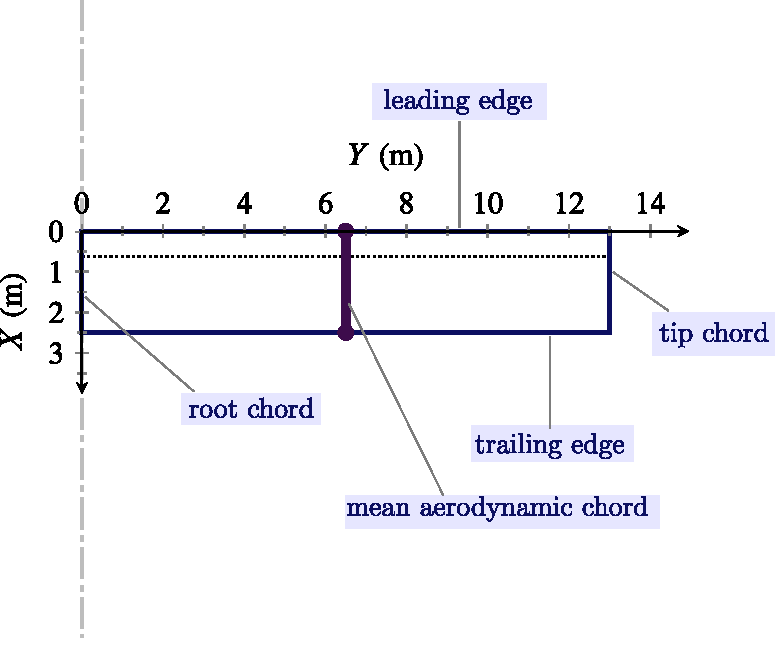
\includegraphics[width=0.78\textwidth]{exercises/wing_planform_basic_0/wing_planform_basic_0_drawing.pdf}%
  \caption{\finalhyphendemerits=1000
           Forma in pianta assegnata nell'esempio~\ref{example:Wing:Basic:AA}.}
  \label{fig:Wing:Planform:Basic:Drawing:AA}%
\end%
    %{figure}%
    {SCfigure}%
%
%\EnlargedFigure% needs two latex passes
%    {t}% #1: t, b, p
%    {images/airfoil_geometry}% #2: the image file included by \includegraphics
%    {width=1.0\textwidth}% #3: option list to pass to \includegraphics, e.g. width=\linewidth,rotate=0
%    {\finalhyphendemerits=1000
%      Alcune caratteristiche geometriche di un profilo alare.}% #4: the caption text
%    {fig:Aero:Profilo:Geometria}% #5: the label
%\EnlargedFigureX% needs two latex passes
%  {t}% #1: t, b, p
%  {%
%    \makebox[\textwidth][c]{%
%    \includegraphics%
%      %[width=0.52\textwidth]%
%      % [height=5.5cm]%
%      [width=0.485\textwidth]%
%      {images/airfoil_Re_effect_polar.pdf}%
%    %\rule{8mm}{0pt}% <-- SPACER
%    \hfill
%    \raisebox{-0.6mm}[0pt][0pt]{%
%    \includegraphics%
%      %[width=0.52\textwidth]%
%      % [height=5.5cm]%
%      [width=0.485\textwidth]%
%      {images/airfoil_Re_effect_alpha_Cl.pdf}
%    }% end-of-raisebox
%    }% end-of-makebox
%  }% #2: the image file included by \includegraphics
%  {\finalhyphendemerits=1000
%    Influenza del numero di Reynolds, $\Reynolds_{\infty}=V_{\!\infty}c/\nu_{\infty}$,
%           sulla polare e sulla curva di portanza di un profilo NACA 64-212.%
%  }% #3: the caption text
%  {fig:Airfoil:Reynolds:Effects}%% #4: the label
%
%-----------------------------------------------------------------------------------------------

\def\mySpanWingMT{10.600000}
\def\mySpanWingIMT{6.360000}
\def\mySpanWingIIMT{4.240000}
\def\myChordRootWingMT{1.440000}
\def\myChordRootWingIMT{1.440000}
\def\myChordRootWingIIMT{1.440000}
\def\myChordTipWingMT{0.860000}
\def\myChordTipWingIMT{1.440000}
\def\myChordTipWingIIMT{0.860000}
\def\mySweepLEWingIIDEG{0.000000}
\def\myCoeffAChordWingI{0.000000}
\def\myCoeffBChordWingIMT{1.440000}
\def\myCoeffAChordWingII{-0.273585}
\def\myCoeffBChordWingIIMT{1.440000}
\def\myAlphaZeroLiftRootWingIDEG{-2.500000}
\def\myAlphaZeroLiftTipWingIDEG{-2.500000}
\def\myAlphaZeroLiftRootWingIRAD{-0.043633}
\def\myAlphaZeroLiftTipWingIRAD{-0.043633}
\def\myAlphaZeroLiftRootWingIIDEG{-2.500000}
\def\myAlphaZeroLiftTipWingIIDEG{-1.000000}
\def\myAlphaZeroLiftRootWingIIRAD{-0.043633}
\def\myAlphaZeroLiftTipWingIIRAD{-0.017453}
\def\myTaperRatioWingI{1.000000}
\def\myTaperRatioWingII{0.597222}
\def\myTwistWingIDEG{0.000000}
\def\myTwistWingIRAD{0.000000}
\def\myTwistWingIIDEG{-3.000000}
\def\myTwistWingIIRAD{-0.052360}
\def\myAreaWingIMTsquared{9.158400}
\def\myAreaWingIIMTsquared{4.876000}
\def\myAreaWingMTsquared{14.034400}
\def\myCoeffAAeroTwistWingIRADMT{0.000000}
\def\myCoeffBAeroTwistWingIRAD{-0.043633}
\def\myCoeffAAeroTwistWingIIRADMT{0.012349}
\def\myCoeffBAeroTwistWingIIRAD{-0.043633}
\def\myCoeffATwistWingIRADMT{0.000000}
\def\myCoeffATwistWingIIRADMT{-0.024698}
\def\myCoeffBTwistWingIRAD{0.000000}
\def\myCoeffBTwistWingIIRAD{0.000000}
\def\myAlphaZeroLiftWingIRAD{-0.028653}
\def\myAlphaZeroLiftWingIDEG{-1.641680}
\def\myAlphaZeroLiftWingIIRAD{0.008329}
\def\myAlphaZeroLiftWingIIDEG{0.477233}
\def\myAlphaZeroLiftWingRAD{-0.020323}
\def\myAlphaZeroLiftWingDEG{-1.164447}

%
\begin{myExampleX}{Caratteristiche geometriche di un'ala dritta}{\ding{46}}% \ \Keyboard\ %
\label{example:Wing:Basic:AA}
%
\noindent
Un'ala finita ha apertura $b=\SI[round-precision=1]{\mySpanWingMT}{\metre}$,
bordi d'attacco e d'uscita rettilinei e
angolo di freccia nullo, cioè $\Lambda_{c/4}=\SI[round-precision=1]{\mySweepQuarterChordWingDEG}{\degree}$.
Inoltre, le sezioni alari alle varie stazioni $Y$ lungo l'apertura hanno corda costante 
pari a $\SI[round-precision=2]{\myChordRootWingMT}{\metre}$
e hanno tutte lo stesso profilo, cioè le caratteristiche aerodinamiche di sezione sono costanti.

Si vogliono calcolare le seguenti grandezze:

\noindent
\adjustbox{center=\textwidth}{%
$S$\,, $\AR$\,, $\bar{c}$\,, $X_{\mathrm{le},\bar{c}}$\,, $Y_{\bar{c}}$
}% \,, $Y_{\bar{c}}$

\medskip
Non essendo rastremata, l'ala ha una corda di radice 
$c_\mathrm{r}=\SI[round-precision=2]{\myChordRootWingMT}{\metre}$,
una corda d'estremità $c_\mathrm{t}=\SI[round-precision=2]{\myChordTipWingMT}{\metre}$
e un rapporto di rastremazione $\lambda=\SI[round-precision=2]{\myTaperRatioWing}{}$.
La freccia del bordo d'attacco è
$\Lambda_\mathrm{le}=\SI[round-precision=1]{\mySweepLEWingDEG}{\degree}$.

La superficie alare si calcola come segue:
\[
\begin{split}
S & {}= \frac{b}{2} \, c_\mathrm{r} \, \big( 1 + \lambda \big) = b\,c_\mathrm{r}\\
  & {}=
    \num{0.5} \cdot \SI[round-precision=1]{\mySpanWingMT}{\metre}
      \cdot \SI[round-precision=2]{\myChordRootWingMT}{\metre}
      \cdot \big( 1 + \SI[round-precision=2]{\myTaperRatioWing}{} \big) 
    = \mathunderline{mydarkblue}{ \SI[round-precision=1]{\myAreaWingMTsquared}{\metre^2} }
\end{split}
\]
In questo caso essa è semplicemente l'area di un rettangolo.

L'allungamento è dunque
\[
\AR 
  = \frac{b^2}{S}
  = \frac{\big(\SI[round-precision=1]{\mySpanWingMT}{\metre}\big)^2}{\SI[round-precision=1]{\myAreaWingMTsquared}{\metre^2}}
  = \mathunderline{mydarkblue}{ \num[round-precision=2]{\myAspectRatioWing} }
\]
Questo valore è superiore a $\num[round-precision=0]{10}$ e permette di affermare che si è in 
presenza di un'ala di elevato allungamento.

La corda media aerodinamica è data dalla formula
\[
\begin{split}
\bar{c} & {}= \frac{2}{3} \, c_\mathrm{r} \, \frac{1+\lambda + \lambda^2}{1+\lambda} \\
  & {}=
    \num{0.667} \cdot \SI[round-precision=2]{\myChordRootWingMT}{\metre}
      \cdot 
        \frac{
          1 + \SI[round-precision=2]{\myTaperRatioWing}{} + \SI[round-precision=2]{\myTaperRatioWing}{}^2
        }{
          1 + \SI[round-precision=2]{\myTaperRatioWing}{}
        }
    = \mathunderline{mydarkblue}{ \SI[round-precision=2]{\myMACWingMT}{\metre} }
\end{split}
\]
Si osserva che per ali di questo tipo il valore di $\bar{c}$ non è altro che quello della corda
di qualsiasi sezione alare.

La distanza longitudinale del bordo d'attacco della corda media aerodinamica dal
bordo d'attacco della corda di radice è data da
\[
\begin{split}
X_{\mathrm{le},\bar{c}} 
  & {}=
    \frac{b}{6} \, \frac{1+2\lambda}{1+\lambda} \tan\Lambda_\mathrm{le} \\[3pt]
  & {}=
    \frac{\SI[round-precision=1]{\mySpanWingMT}{\metre}}{6}
      \cdot 
      \frac{
        1 + 2\cdot\SI[round-precision=2]{\myTaperRatioWing}{}
      }{
        1 + \SI[round-precision=2]{\myTaperRatioWing}{}
      }
      \cdot \tan \big( \SI[round-precision=3]{\mySweepLEWingRAD}{\radian} \big)
    = \mathunderline{mydarkblue}{ \SI[round-precision=2]{\myXMACLEToApexWingMT}{\metre} }% \myXMACLEToWingRootLEMT
\end{split}
\]
Il valore nullo conferma che la corda media aerodinamica, proiettata sul piano di mezzeria
dell'ala, si sovrappone alla corda di radice.

Per l'ala assegnata tutte le stazioni $Y$ lungo l'aperture hanno corda pari a $\bar{c}$.
Formalmente, la stazione $Y_{\bar{c}}$ corrispondente alla corda media aerodinamica 
si calcola come segue:
\[
\begin{split}
Y_{\bar{c}} 
  & {}=
    \frac{b}{6} \, \frac{1+2\lambda}{1+\lambda} = \\[3pt]
  & {}=
    \frac{\SI[round-precision=1]{\mySpanWingMT}{\metre}}{6}
      \cdot 
      \frac{
        1 + 2\cdot\SI[round-precision=2]{\myTaperRatioWing}{}
      }{
        1 + \SI[round-precision=2]{\myTaperRatioWing}{}
      }
    = \mathunderline{mydarkblue}{ \SI[round-precision=2]{\myYMACWingMT}{\metre} }
    = \frac{b}{2} \, \frac{1}{2}
\end{split}
\]
Il valore ottenuto corrisponde alla stazione lungo l'apertura alare a metà strada tra la
la corda di radice e la corda d'estremità.

Si vedrà più avanti che per questo tipo di ala dritta a sezione costante, quando lo svergolamento 
geometrico  $\epsilon_\mathrm{g}(Y)$ è identicamente nullo, 
le caratteristiche aerodinamiche basilari del profilo di sezione si trasferiscono all'ala finita.
Per esempio, l'angolo di portanza nulla $\alpha_{0L}$ coincide con l'angolo $\alpha_{0\ell}$
di portanza nulla del profilo; così come $C_L\big|_{\alpha=0}$ coincide con il $C_{\ell 0}$ di profilo.
Il gradiente \smash{$C_{L_\mathlarger{\alpha}}$} relativo all'ala va invece corretto rispetto al 
valore \smash{$C_{\ell_\mathlarger{\alpha}}$} relativo al profilo per l'effetto dell'allungamento finito.

\end{myExampleX}
%--END-EXERCISE:wing_planform_basic_0
%===============================================================================================

%===============================================================================================
%--BEGIN-EXERCISE:wing_planform_basic_0_A
%
\def\mySpanWingMT{10.600000}
\def\mySpanWingIMT{6.360000}
\def\mySpanWingIIMT{4.240000}
\def\myChordRootWingMT{1.440000}
\def\myChordRootWingIMT{1.440000}
\def\myChordRootWingIIMT{1.440000}
\def\myChordTipWingMT{0.860000}
\def\myChordTipWingIMT{1.440000}
\def\myChordTipWingIIMT{0.860000}
\def\mySweepLEWingIIDEG{0.000000}
\def\myCoeffAChordWingI{0.000000}
\def\myCoeffBChordWingIMT{1.440000}
\def\myCoeffAChordWingII{-0.273585}
\def\myCoeffBChordWingIIMT{1.440000}
\def\myAlphaZeroLiftRootWingIDEG{-2.500000}
\def\myAlphaZeroLiftTipWingIDEG{-2.500000}
\def\myAlphaZeroLiftRootWingIRAD{-0.043633}
\def\myAlphaZeroLiftTipWingIRAD{-0.043633}
\def\myAlphaZeroLiftRootWingIIDEG{-2.500000}
\def\myAlphaZeroLiftTipWingIIDEG{-1.000000}
\def\myAlphaZeroLiftRootWingIIRAD{-0.043633}
\def\myAlphaZeroLiftTipWingIIRAD{-0.017453}
\def\myTaperRatioWingI{1.000000}
\def\myTaperRatioWingII{0.597222}
\def\myTwistWingIDEG{0.000000}
\def\myTwistWingIRAD{0.000000}
\def\myTwistWingIIDEG{-3.000000}
\def\myTwistWingIIRAD{-0.052360}
\def\myAreaWingIMTsquared{9.158400}
\def\myAreaWingIIMTsquared{4.876000}
\def\myAreaWingMTsquared{14.034400}
\def\myCoeffAAeroTwistWingIRADMT{0.000000}
\def\myCoeffBAeroTwistWingIRAD{-0.043633}
\def\myCoeffAAeroTwistWingIIRADMT{0.012349}
\def\myCoeffBAeroTwistWingIIRAD{-0.043633}
\def\myCoeffATwistWingIRADMT{0.000000}
\def\myCoeffATwistWingIIRADMT{-0.024698}
\def\myCoeffBTwistWingIRAD{0.000000}
\def\myCoeffBTwistWingIIRAD{0.000000}
\def\myAlphaZeroLiftWingIRAD{-0.028653}
\def\myAlphaZeroLiftWingIDEG{-1.641680}
\def\myAlphaZeroLiftWingIIRAD{0.008329}
\def\myAlphaZeroLiftWingIIDEG{0.477233}
\def\myAlphaZeroLiftWingRAD{-0.020323}
\def\myAlphaZeroLiftWingDEG{-1.164447}

%
\begin{myExampleX}{Caratteristiche geometriche di un'ala dritta e rastremata}{\ding{46}}% \ \Keyboard\ %
\label{example:Wing:Basic:AB}
%
\noindent
Un'ala finita ha apertura $b=\SI[round-precision=1]{\mySpanWingMT}{\metre}$,
bordi d'attacco e d'uscita rettilinei e
angolo di freccia nullo, cioè $\Lambda_{c/4}=\SI[round-precision=1]{\mySweepQuarterChordWingDEG}{\degree}$.
A differenza dell'esempio~\ref{example:Wing:Basic:AA}, l'ala assegnata qui è rastremata, cioè
la corda delle diverse sezioni alari varia linearmente con la distanza $Y$ dal piano di mezzeria.
La corda di radice è $c_\mathrm{r}=\SI[round-precision=2]{\myChordRootWingMT}{\metre}$ e
la corda d'estremità è $c_\mathrm{t}=\SI[round-precision=2]{\myChordTipWingMT}{\metre}$.

Si vogliono calcolare le seguenti grandezze:

\noindent
\adjustbox{center=\textwidth}{%
$S$\,, $\AR$\,, $\Lambda_\mathrm{le}$\,, $\bar{c}$\,, $X_{\mathrm{le},\bar{c}}$\,, $Y_{\bar{c}}$
}% \,, $Y_{\bar{c}}$

\medskip
Date le due corde di radice e d'estremità, va valutato il rapporto di rastremazione
\[
\lambda
  =\frac{c_\mathrm{t}}{c_\mathrm{r}}
  =\frac{\SI[round-precision=2]{\myChordTipWingMT}{\metre}}{\SI[round-precision=2]{\myChordRootWingMT}{\metre}}
  =\mathunderline{mydarkblue}{ \SI[round-precision=2]{\myTaperRatioWing}{} }
\]

Per quanto riguarda la legge delle corde, si pone
$c ( Y ) = A_c \, Y + B_c$. Imponendo che $c(0)=c_\mathrm{r}$ e $c(\frac{1}{2}b)=c_\mathrm{t}$,
si ha che i coefficienti della legge lineare sono
\[
A_c
  = \frac{c_\mathrm{t} - c_\mathrm{r}}{b/2}
  = 
    2 \frac{
      \SI[round-precision=2]{\myChordTipWingMT}{\metre} - \SI[round-precision=2]{\myChordRootWingMT}{\metre}
    }{
      \SI[round-precision=2]{\mySpanWingMT}{\metre}
    }
  = \mathunderline{mydarkblue}{ \SI[round-precision=3]{\myCoeffAChordWing}{} }
\]
\[
B_c
  = c_\mathrm{r}
  = \mathunderline{mydarkblue}{ \SI[round-precision=2]{\myCoeffBChordWingMT}{\metre} }
\]
Dunque
\[
c \big( Y \big) = A_c \, Y + B_c
  = \SI[round-precision=3]{\myCoeffAChordWing}{} \, Y
    + \SI[round-precision=2]{\myCoeffBChordWingMT}{\metre}
\]

La superficie alare in questo caso non è altro che l'area di due trapezi,
ciascuno di base maggiore $c_\mathrm{r}$, base minore $c_\mathrm{t}$ e altezza $\frac{1}{2}b$,
e si calcola come segue:
\[
\begin{split}
S & {}= \frac{b}{2} \, c_\mathrm{r} \, \big( 1 + \lambda \big) \\
  & {}=
    \num{0.5} \cdot \SI[round-precision=1]{\mySpanWingMT}{\metre}
      \cdot \SI[round-precision=2]{\myChordRootWingMT}{\metre}
      \cdot \big( 1 + \SI[round-precision=2]{\myTaperRatioWing}{} \big) 
    = \mathunderline{mydarkblue}{ \SI[round-precision=1]{\myAreaWingMTsquared}{\metre^2} }
\end{split}
\]
È facile verificare che si ottiene lo stesso risultato se si applica la formula di calcolo
\[
\begin{split}
S & {}= 2\, \int_0^{b/2} c(Y) \diff{Y} = 2\, \int_0^{b/2} \Big( A_c Y + B_c \Big) \diff{Y}
\\
  & {}= 2\, 
    \int_{\SI{0}{m}}^{\calcSI[round-precision=1,fixed-exponent=0,scientific-notation=fixed]{0.5*\mySpanWingMT}{\metre}}
    \Big( 
      \SI[round-precision=3]{\myCoeffAChordWing}{} \, Y
      + \SI[round-precision=2]{\myCoeffBChordWingMT}{\metre}
    \Big) \diff{Y}
    = 2\, \bigg[
      \SI[round-precision=3]{\myCoeffAChordWing}{} \, \dfrac{Y^2}{2}
      + \SI[round-precision=2]{\myCoeffBChordWingMT}{\metre} \, Y
    \bigg]_{\SI{0}{m}}^{\calcSI[round-precision=1,fixed-exponent=0,scientific-notation=fixed]{0.5*\mySpanWingMT}{\metre}}
\\
  & {}= 2\,
    \Big(
      \SI[round-precision=3]{\myCoeffAChordWing}{}
        \cdot 
        \calcSI[round-precision=1,fixed-exponent=0,scientific-notation=fixed]{
          0.5*\mySpanWingMT*0.5*\mySpanWingMT*0.5
        }{\metre^2}
        + 
        \calcSI[round-precision=1,fixed-exponent=0,scientific-notation=fixed]{
          \myCoeffBChordWingMT * 0.5*\mySpanWingMT
        }{\metre^2}
    \Big) - \SI{0}{\metre^2}
\end{split}
\]

A questo punto si può calcolare l'allungamento alare, che è
\[
\AR
  = \frac{b^2}{S}
  = \frac{\big(\SI[round-precision=1]{\mySpanWingMT}{\metre}\big)^2}{\SI[round-precision=1]{\myAreaWingMTsquared}{\metre^2}}
  = \mathunderline{mydarkblue}{ \num[round-precision=2]{\myAspectRatioWing} }
\]

È noto che la linea congiungente i punti lungo le singole corde $c(Y)$ distanti 
$c(Y)/n$ dal bordo d'attacco locale forma un angolo di freccia $\Lambda_{c/n}$ collegato a quello 
del bordo d'attacco $\Lambda_\mathrm{le}$ dalla seguente relazione:
\[
\tan\Lambda_{c/n} = \tan\Lambda_\mathrm{le}-\dfrac{(4/n)(1-\lambda)}{\AR(1+\lambda)}
\]
Da questa, per una freccia
$\Lambda_\mathrm{c/4}=\SI[round-precision=1]{\mySweepQuarterChordWingDEG}{\degree}$
della linea dei quarti di corda, si ricava
\[
\tan
\SI[round-precision=1]{\mySweepQuarterChordWingRAD}{}
   = \tan\Lambda_\mathrm{le} 
      - \dfrac{
         \num[round-precision=2]{1.0}
         \cdot (1-\SI[round-precision=2]{\myTaperRatioWing}{})
      }{
         \num[round-precision=2]{\myAspectRatioWing}
         \cdot (1+\SI[round-precision=2]{\myTaperRatioWing}{})} 
   \quad
   \Rightarrow
   \quad
   \Lambda_\mathrm{le}
      = \mathunderline{mydarkblue}{ \SI[round-precision=4]{\mySweepLEWingRAD}{\radian} }
      = \mathunderline{mydarkblue}{ \SI[round-precision=1]{\mySweepLEWingDEG}{\deg} }
\]

La corda media aerodinamica è in questo caso
\[
\begin{split}
\bar{c} & {}= \frac{2}{3} \, c_\mathrm{r} \, \frac{1+\lambda + \lambda^2}{1+\lambda} \\
  & {}=
    \num{0.667} \cdot \SI[round-precision=2]{\myChordRootWingMT}{\metre}
      \cdot 
        \frac{
          1 + \SI[round-precision=2]{\myTaperRatioWing}{} + \SI[round-precision=2]{\myTaperRatioWing}{}^2
        }{
          1 + \SI[round-precision=2]{\myTaperRatioWing}{}
        }
    = \mathunderline{mydarkblue}{ \SI[round-precision=2]{\myMACWingMT}{\metre} }
\end{split}
\]
cioè un valore intermedio tra quello della corda di radice (\SI[round-precision=2]{\myChordRootWingMT}{\metre}) 
e quello della corda d'estremità (\SI[round-precision=2]{\myChordTipWingMT}{\metre}),
più vicino al primo che che al secondo.

La distanza longitudinale del bordo d'attacco della corda media aerodinamica dal
bordo d'attacco della corda di radice è
\[
\begin{split}
X_{\mathrm{le},\bar{c}} 
  & {}=
    \frac{b}{6} \, \frac{1+2\lambda}{1+\lambda} \tan\Lambda_\mathrm{le} \\[3pt]
  & {}=
    \frac{\SI[round-precision=1]{\mySpanWingMT}{\metre}}{6}
      \cdot 
      \frac{
        1 + 2\cdot\SI[round-precision=2]{\myTaperRatioWing}{}
      }{
        1 + \SI[round-precision=2]{\myTaperRatioWing}{}
      }
      \cdot \tan \big( \SI[round-precision=3]{\mySweepLEWingRAD}{\radian} \big)
    = \mathunderline{mydarkblue}{ \SI[round-precision=2]{\myXMACLEToApexWingMT}{\metre} }% \myXMACLEToWingRootLEMT
\end{split}
\]
Si osserva che all'ala rastremata, pur se di freccia nulla, corrisponde un
$X_{\mathrm{le},\bar{c}}$ non nullo. Ciò significa che la proiezione della sezione alare avente 
corda pari a $\bar{c}$ nel piano di mezzeria è più arretrata della corda di radice.
Inoltre, dato il valore di $\bar{c}$ precedentemente calcolato, tale proiezione
è tutta interna alla corda di radice, cioè
$X_{\mathrm{le},\bar{c}}+\bar{c}<c_\mathrm{r}$.
Per una conferma grafica di questi risultati 
si veda la figura~\ref{fig:Wing:Planform:Basic:Drawing:AB}.

La stazione $Y_{\bar{c}}$ alla quale la legge delle corde $c(Y)$ assume il valore $\bar{c}$ è
\[
\begin{split}
Y_{\bar{c}} 
  & {}=
    \frac{b}{6} \, \frac{1+2\lambda}{1+\lambda} = \\[3pt]
  & {}=
    \frac{\SI[round-precision=1]{\mySpanWingMT}{\metre}}{6}
      \cdot 
      \frac{
        1 + 2\cdot\SI[round-precision=2]{\myTaperRatioWing}{}
      }{
        1 + \SI[round-precision=2]{\myTaperRatioWing}{}
      }
    = \mathunderline{mydarkblue}{ \SI[round-precision=2]{\myYMACWingMT}{\metre} }
\end{split}
\]
Il valore calcolato corrisponde a una stazione lungo l'apertura alare più vicina alla radice che
all'estremità.

\end{myExampleX}

%-----------------------------------------------------------------------------------------------
\begin%
  %{figure}
  {SCfigure}[1.9]%
  [t]%[H]%[!htbp]
  %\centering
  %\checkoddpage
  %\centering
    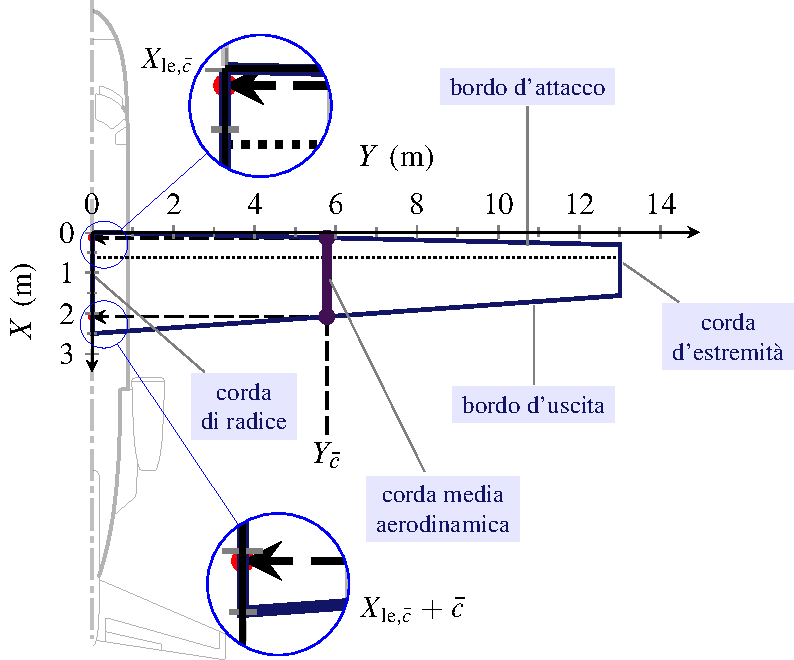
\includegraphics[width=0.78\textwidth]{exercises/wing_planform_basic_0A/wing_planform_basic_0A_drawing.pdf}%
  \caption{\finalhyphendemerits=1000
           Forma in pianta assegnata nell'esempio~\ref{example:Wing:Basic:AB}.}
  \label{fig:Wing:Planform:Basic:Drawing:AB}%
\end%
    %{figure}%
    {SCfigure}%
%
%\EnlargedFigure% needs two latex passes
%    {t}% #1: t, b, p
%    {images/airfoil_geometry}% #2: the image file included by \includegraphics
%    {width=1.0\textwidth}% #3: option list to pass to \includegraphics, e.g. width=\linewidth,rotate=0
%    {\finalhyphendemerits=1000
%      Alcune caratteristiche geometriche di un profilo alare.}% #4: the caption text
%    {fig:Aero:Profilo:Geometria}% #5: the label
%\EnlargedFigureX% needs two latex passes
%  {t}% #1: t, b, p
%  {%
%    \makebox[\textwidth][c]{%
%    \includegraphics%
%      %[width=0.52\textwidth]%
%      % [height=5.5cm]%
%      [width=0.485\textwidth]%
%      {images/airfoil_Re_effect_polar.pdf}%
%    %\rule{8mm}{0pt}% <-- SPACER
%    \hfill
%    \raisebox{-0.6mm}[0pt][0pt]{%
%    \includegraphics%
%      %[width=0.52\textwidth]%
%      % [height=5.5cm]%
%      [width=0.485\textwidth]%
%      {images/airfoil_Re_effect_alpha_Cl.pdf}
%    }% end-of-raisebox
%    }% end-of-makebox
%  }% #2: the image file included by \includegraphics
%  {\finalhyphendemerits=1000
%    Influenza del numero di Reynolds, $\Reynolds_{\infty}=V_{\!\infty}c/\nu_{\infty}$,
%           sulla polare e sulla curva di portanza di un profilo NACA 64-212.%
%  }% #3: the caption text
%  {fig:Airfoil:Reynolds:Effects}%% #4: the label
%
%-----------------------------------------------------------------------------------------------

%--END-EXERCISE:wing_planform_basic_0_A
%===============================================================================================

%===============================================================================================
%--BEGIN-EXERCISE:wing_planform_basic_1
%
\def\mySpanWingMT{10.600000}
\def\mySpanWingIMT{6.360000}
\def\mySpanWingIIMT{4.240000}
\def\myChordRootWingMT{1.440000}
\def\myChordRootWingIMT{1.440000}
\def\myChordRootWingIIMT{1.440000}
\def\myChordTipWingMT{0.860000}
\def\myChordTipWingIMT{1.440000}
\def\myChordTipWingIIMT{0.860000}
\def\mySweepLEWingIIDEG{0.000000}
\def\myCoeffAChordWingI{0.000000}
\def\myCoeffBChordWingIMT{1.440000}
\def\myCoeffAChordWingII{-0.273585}
\def\myCoeffBChordWingIIMT{1.440000}
\def\myAlphaZeroLiftRootWingIDEG{-2.500000}
\def\myAlphaZeroLiftTipWingIDEG{-2.500000}
\def\myAlphaZeroLiftRootWingIRAD{-0.043633}
\def\myAlphaZeroLiftTipWingIRAD{-0.043633}
\def\myAlphaZeroLiftRootWingIIDEG{-2.500000}
\def\myAlphaZeroLiftTipWingIIDEG{-1.000000}
\def\myAlphaZeroLiftRootWingIIRAD{-0.043633}
\def\myAlphaZeroLiftTipWingIIRAD{-0.017453}
\def\myTaperRatioWingI{1.000000}
\def\myTaperRatioWingII{0.597222}
\def\myTwistWingIDEG{0.000000}
\def\myTwistWingIRAD{0.000000}
\def\myTwistWingIIDEG{-3.000000}
\def\myTwistWingIIRAD{-0.052360}
\def\myAreaWingIMTsquared{9.158400}
\def\myAreaWingIIMTsquared{4.876000}
\def\myAreaWingMTsquared{14.034400}
\def\myCoeffAAeroTwistWingIRADMT{0.000000}
\def\myCoeffBAeroTwistWingIRAD{-0.043633}
\def\myCoeffAAeroTwistWingIIRADMT{0.012349}
\def\myCoeffBAeroTwistWingIIRAD{-0.043633}
\def\myCoeffATwistWingIRADMT{0.000000}
\def\myCoeffATwistWingIIRADMT{-0.024698}
\def\myCoeffBTwistWingIRAD{0.000000}
\def\myCoeffBTwistWingIIRAD{0.000000}
\def\myAlphaZeroLiftWingIRAD{-0.028653}
\def\myAlphaZeroLiftWingIDEG{-1.641680}
\def\myAlphaZeroLiftWingIIRAD{0.008329}
\def\myAlphaZeroLiftWingIIDEG{0.477233}
\def\myAlphaZeroLiftWingRAD{-0.020323}
\def\myAlphaZeroLiftWingDEG{-1.164447}

%
\begin{myExampleX}{Caratteristiche di un'ala a bordi dritti, rastremata, a freccia}{\ding{46}}% \ \Keyboard\ %
\label{example:Wing:Basic:A}
%
\noindent
L'ala di un velivolo ha bordi d'attacco e d'uscita rettilinei,
apertura $b=\SI[round-precision=1]{\mySpanWingMT}{\metre}$,
corda di radice $c_\mathrm{r}=\SI[round-precision=2]{\myChordRootWingMT}{\metre}$,
corda d'estremità $c_\mathrm{t}=\SI[round-precision=2]{\myChordTipWingMT}{\metre}$
e freccia del bordo d'attacco
$\Lambda_\mathrm{le}=\SI[round-precision=1]{\mySweepLEWingDEG}{\degree}$.

Si vogliono calcolare le seguenti grandezze:

\noindent
\adjustbox{center=\textwidth}{%
$S$\,, $\AR$\,, $\Lambda_{c/4}$\,, $\Lambda_{c/2}$\,, $\Lambda_\mathrm{te}$\,, 
$\bar{c}$\,, $X_{\mathrm{le},\bar{c}}$\,, $Y_{\bar{c}}$
}% \,, $Y_{\bar{c}}$

\medskip
Per le corde di sezione vale la legge lineare
$c \big( Y \big) = A_c \, Y + B_c$ 
con
\[
A_c
  = \frac{c_\mathrm{t} - c_\mathrm{r}}{b/2}
  = 
    2 \frac{
      \SI[round-precision=2]{\myChordTipWingMT}{\metre} - \SI[round-precision=2]{\myChordRootWingMT}{\metre}
    }{
      \SI[round-precision=2]{\mySpanWingMT}{\metre}
    }
  = \mathunderline{mydarkblue}{ \SI[round-precision=3]{\myCoeffAChordWing}{} }
\]
\[
B_c
  = c_\mathrm{r}
  = \mathunderline{mydarkblue}{ \SI[round-precision=2]{\myCoeffBChordWingMT}{\metre} }
\]
dunque
\[
c \big( Y \big) = A_c \, Y + B_c
  = \SI[round-precision=3]{\myCoeffAChordWing}{} \, Y
    + \SI[round-precision=2]{\myCoeffBChordWingMT}{\metre}
\]

Il rapporto di rastremazione è
\[
\lambda
  =\frac{c_\mathrm{t}}{c_\mathrm{r}}
  =\frac{\SI[round-precision=2]{\myChordTipWingMT}{\metre}}{\SI[round-precision=2]{\myChordRootWingMT}{\metre}}
  =\mathunderline{mydarkblue}{ \SI[round-precision=2]{\myTaperRatioWing}{} }
\]
e la superficie alare è
\[
\begin{split}
S & {}= \frac{b}{2} \, c_\mathrm{r} \, \big( 1 + \lambda \big) \\
  & {}=
    \num{0.5} \cdot \SI[round-precision=1]{\mySpanWingMT}{\metre}
      \cdot \SI[round-precision=2]{\myChordRootWingMT}{\metre}
      \cdot \big( 1 + \SI[round-precision=2]{\myTaperRatioWing}{} \big) 
    = \mathunderline{mydarkblue}{ \SI[round-precision=1]{\myAreaWingMTsquared}{\metre^2} }
\end{split}
\]
Ne consegue un allungamento alare
\[
\AR
  = \frac{b^2}{S}
  = \frac{\big(\SI[round-precision=1]{\mySpanWingMT}{\metre}\big)^2}{\SI[round-precision=1]{\myAreaWingMTsquared}{\metre^2}}
  = \mathunderline{mydarkblue}{ \num[round-precision=2]{\myAspectRatioWing} }
\]

Per la relazione
\[
\tan\Lambda_{c/n} = \tan\Lambda_\mathrm{le}-\dfrac{(4/n)(1-\lambda)}{\AR(1+\lambda)}
\]
che lega l'angolo di freccia del bordo d'attacco $\Lambda_\mathrm{le}$ all'angolo di freccia 
$\Lambda_{c/n}$ della linea congiungente i punti lungo le singole corde $c(Y)$ distanti $c(Y)/n$ 
dal bordo d'attacco locale, si ha
\[
\tan
\Lambda_{c/4}
   = \tan (\SI[round-precision=3]{\mySweepLEWingRAD}{\radian})
      - \dfrac{
         \num[round-precision=2]{1.0}
         \cdot (1-\SI[round-precision=2]{\myTaperRatioWing}{})
      }{
         \num[round-precision=2]{\myAspectRatioWing}
         \cdot (1+\SI[round-precision=2]{\myTaperRatioWing}{})} 
   \quad
   \Rightarrow
   \quad
   \Lambda_{c/4}
      = \mathunderline{mydarkblue}{ \SI[round-precision=3]{\mySweepQuarterChordWingRAD}{\radian} }
      = \mathunderline{mydarkblue}{ \SI[round-precision=1]{\mySweepQuarterChordWingDEG}{\deg} }
\]

\[
\tan
\Lambda_{c/2}
   = \tan (\SI[round-precision=3]{\mySweepLEWingRAD}{\radian})
      - \dfrac{
         \num[round-precision=2]{2.0}
         \cdot (1-\SI[round-precision=2]{\myTaperRatioWing}{})
      }{
         \num[round-precision=2]{\myAspectRatioWing}
         \cdot (1+\SI[round-precision=2]{\myTaperRatioWing}{})} 
   \quad
   \Rightarrow
   \quad
   \Lambda_{c/2}
      = \mathunderline{mydarkblue}{ \SI[round-precision=3]{\mySweepHalfChordWingRAD}{\radian} }
      = \mathunderline{mydarkblue}{ \SI[round-precision=1]{\mySweepHalfChordWingDEG}{\deg} }
\]

\[
\tan
\Lambda_\mathrm{te}
   = \tan (\SI[round-precision=3]{\mySweepLEWingRAD}{\radian})
      - \dfrac{
         \num[round-precision=2]{4.0}
         \cdot (1-\SI[round-precision=2]{\myTaperRatioWing}{})
      }{
         \num[round-precision=2]{\myAspectRatioWing}
         \cdot (1+\SI[round-precision=2]{\myTaperRatioWing}{})} 
   \quad
   \Rightarrow
   \quad
   \Lambda_\mathrm{te}
      = \mathunderline{mydarkblue}{ \SI[round-precision=3]{\mySweepTEWingRAD}{\radian} }
      = \mathunderline{mydarkblue}{ \SI[round-precision=1]{\mySweepTEWingDEG}{\deg} }
\]
Si osserva che gli angoli di freccia caratteristici della forma in pianta vanno progressivamente
a diminuire passando dal bordo d'attacco ($\Lambda_\mathrm{le}$), 
alla linea dei quarti di corda ($\Lambda_{c/4}$),
alla linea mediana ($\Lambda_{c/2}$),
fino al bordo d'uscita ($\Lambda_\mathrm{te}$).

Il valore della corda media aerodinamica è il seguente:
\[
\begin{split}
\bar{c} & {}= \frac{2}{3} \, c_\mathrm{r} \, \frac{1+\lambda + \lambda^2}{1+\lambda} \\
  & {}=
    \num{0.667} \cdot \SI[round-precision=2]{\myChordRootWingMT}{\metre}
      \cdot 
        \frac{
          1 + \SI[round-precision=2]{\myTaperRatioWing}{} + \SI[round-precision=2]{\myTaperRatioWing}{}^2
        }{
          1 + \SI[round-precision=2]{\myTaperRatioWing}{}
        }
    = \mathunderline{mydarkblue}{ \SI[round-precision=2]{\myMACWingMT}{\metre} }
\end{split}
\]

La distanza longitudinale del bordo d'attacco della corda media aerodinamica dal
bordo d'attacco della corda di radice è
\[
\begin{split}
X_{\mathrm{le},\bar{c}} 
  & {}=
    \frac{b}{6} \, \frac{1+2\lambda}{1+\lambda} \tan\Lambda_\mathrm{le} \\[3pt]
  & {}=
    \frac{\SI[round-precision=1]{\mySpanWingMT}{\metre}}{6}
      \cdot 
      \frac{
        1 + 2\cdot\SI[round-precision=2]{\myTaperRatioWing}{}
      }{
        1 + \SI[round-precision=2]{\myTaperRatioWing}{}
      }
      \cdot \tan \big( \SI[round-precision=3]{\mySweepLEWingRAD}{\radian} \big)
    = \mathunderline{mydarkblue}{ \SI[round-precision=2]{\myXMACLEToApexWingMT}{\metre} }% \myXMACLEToWingRootLEMT
\end{split}
\]
Si osserva che per un'ala rastremata e a freccia non nulla si ha un
$X_{\mathrm{le},\bar{c}}$ non nullo. Ciò significa che la proiezione della sezione alare avente 
corda pari a $\bar{c}$ nel piano di mezzeria è più arretrata della corda di radice.
Inoltre, dato il valore di $\bar{c}$ precedentemente calcolato, tale proiezione
non è tutta interna alla corda di radice ma ha un bordo d'uscita di ascissa
$X_{\mathrm{le},\bar{c}}+\bar{c}>c_\mathrm{r}$.
Per una conferma grafica di questi risultati 
si veda la figura~\ref{fig:Wing:Planform:Results:A}.

La stazione $Y_{\bar{c}}$ alla quale la legge delle corde $c(Y)$ assume il valore $\bar{c}$ è
\[
\begin{split}
Y_{\bar{c}} 
  & {}=
    \frac{b}{6} \, \frac{1+2\lambda}{1+\lambda} \\[3pt]
  & {}=
    \frac{\SI[round-precision=1]{\mySpanWingMT}{\metre}}{6}
      \cdot 
      \frac{
        1 + 2\cdot\SI[round-precision=2]{\myTaperRatioWing}{}
      }{
        1 + \SI[round-precision=2]{\myTaperRatioWing}{}
      }
    = \mathunderline{mydarkblue}{ \SI[round-precision=2]{\myYMACWingMT}{\metre} }
\end{split}
\]

Il punto di coordinate $(X_{\mathrm{le},\bar{c}},0)$ è di estrema importanza nella formulazione
delle equazioni di equilibrio al beccheggio e della condizione di stabilità statica al
beccheggio dei velivoli. Tale punto viene preso come riferimento dai progettisti per
valutare la posizione del baricentro e dei centri aerodinamici caratteristici del velivolo
(dell'ala isolata, della configurazione ala-fusoliera, del velivolo completo).
Per esempio, se un dato punto caratteristico $P$ ha una distanza longitudinale 
$a\bar{c}$ dal bordo d'attacco della corda media aerodinamica (con $a$ adimensionale), 
si introduce una coordinata $x$ tale che $x_P = X_P - X_{\mathrm{le},\bar{c}} = a\bar{c}$.
Si dice anche che la posizione adimensionale di $P$ rispetto al bordo d'attacco della corda 
media aerodinamica è $\bar{x}_P=a$.

\end{myExampleX}

%-----------------------------------------------------------------------------------------------
\begin%
  %{figure}
  {SCfigure}[1.9]%
  [t]%[H]%[!htbp]
  %\centering
  %\checkoddpage
  %\centering
    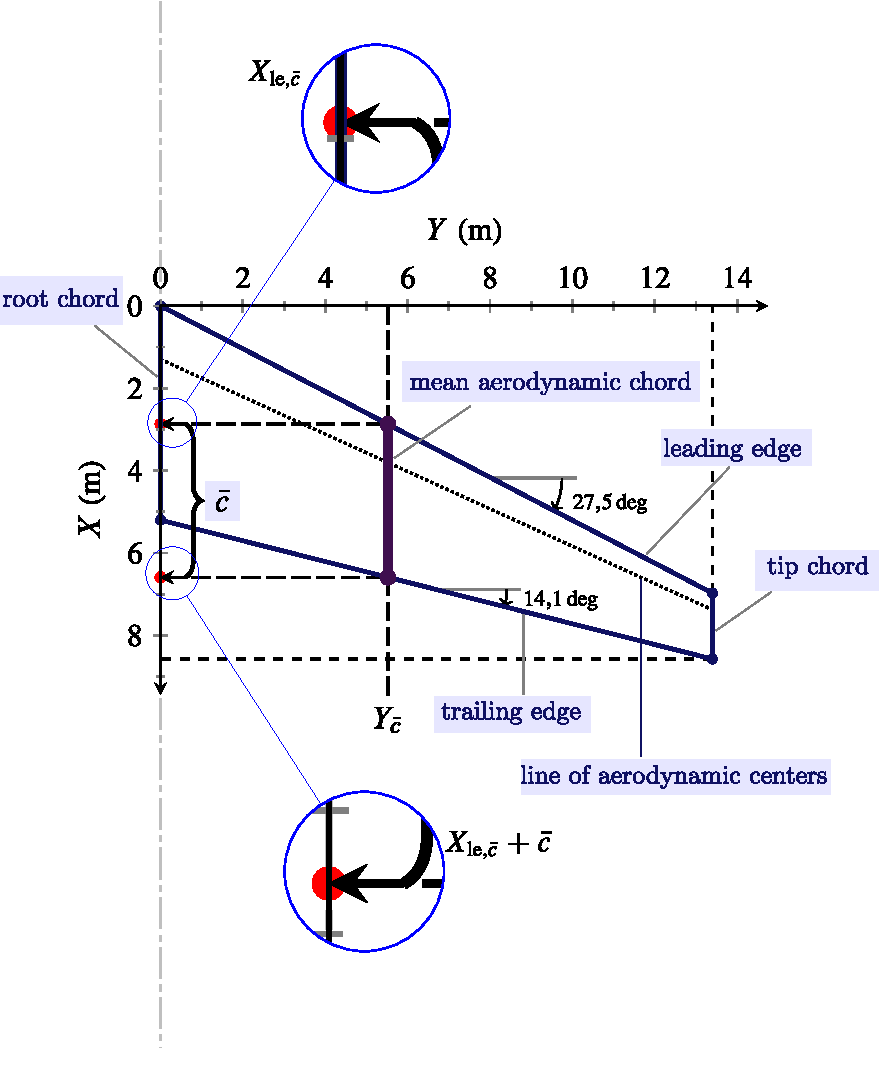
\includegraphics[width=0.78\textwidth]{exercises/wing_planform_basic_1/wing_planform_basic_1_drawing.pdf}%
  \caption{\finalhyphendemerits=1000
           Forma in pianta dell'ala assegnata nell'esempio~\ref{example:Wing:Basic:A}.}
  \label{fig:Wing:Planform:Results:A}%
\end%
    %{figure}%
    {SCfigure}%
%
%\EnlargedFigure% needs two latex passes
%    {t}% #1: t, b, p
%    {images/airfoil_geometry}% #2: the image file included by \includegraphics
%    {width=1.0\textwidth}% #3: option list to pass to \includegraphics, e.g. width=\linewidth,rotate=0
%    {\finalhyphendemerits=1000
%      Alcune caratteristiche geometriche di un profilo alare.}% #4: the caption text
%    {fig:Aero:Profilo:Geometria}% #5: the label
%\EnlargedFigureX% needs two latex passes
%  {t}% #1: t, b, p
%  {%
%    \makebox[\textwidth][c]{%
%    \includegraphics%
%      %[width=0.52\textwidth]%
%      % [height=5.5cm]%
%      [width=0.485\textwidth]%
%      {images/airfoil_Re_effect_polar.pdf}%
%    %\rule{8mm}{0pt}% <-- SPACER
%    \hfill
%    \raisebox{-0.6mm}[0pt][0pt]{%
%    \includegraphics%
%      %[width=0.52\textwidth]%
%      % [height=5.5cm]%
%      [width=0.485\textwidth]%
%      {images/airfoil_Re_effect_alpha_Cl.pdf}
%    }% end-of-raisebox
%    }% end-of-makebox
%  }% #2: the image file included by \includegraphics
%  {\finalhyphendemerits=1000
%    Influenza del numero di Reynolds, $\Reynolds_{\infty}=V_{\!\infty}c/\nu_{\infty}$,
%           sulla polare e sulla curva di portanza di un profilo NACA 64-212.%
%  }% #3: the caption text
%  {fig:Airfoil:Reynolds:Effects}%% #4: the label
%
%-----------------------------------------------------------------------------------------------

%--END-EXERCISE:wing_planform_basic_1
%===============================================================================================

%===============================================================================================
%--BEGIN-EXERCISE:wing_planform_basic_2
%
%-----------------------------------------------------------------------------------------------
\begin%
  %{figure}
  {SCfigure}[1.9]%
  [t]%[H]%[!htbp]
  %\centering
  %\checkoddpage
  %\centering
    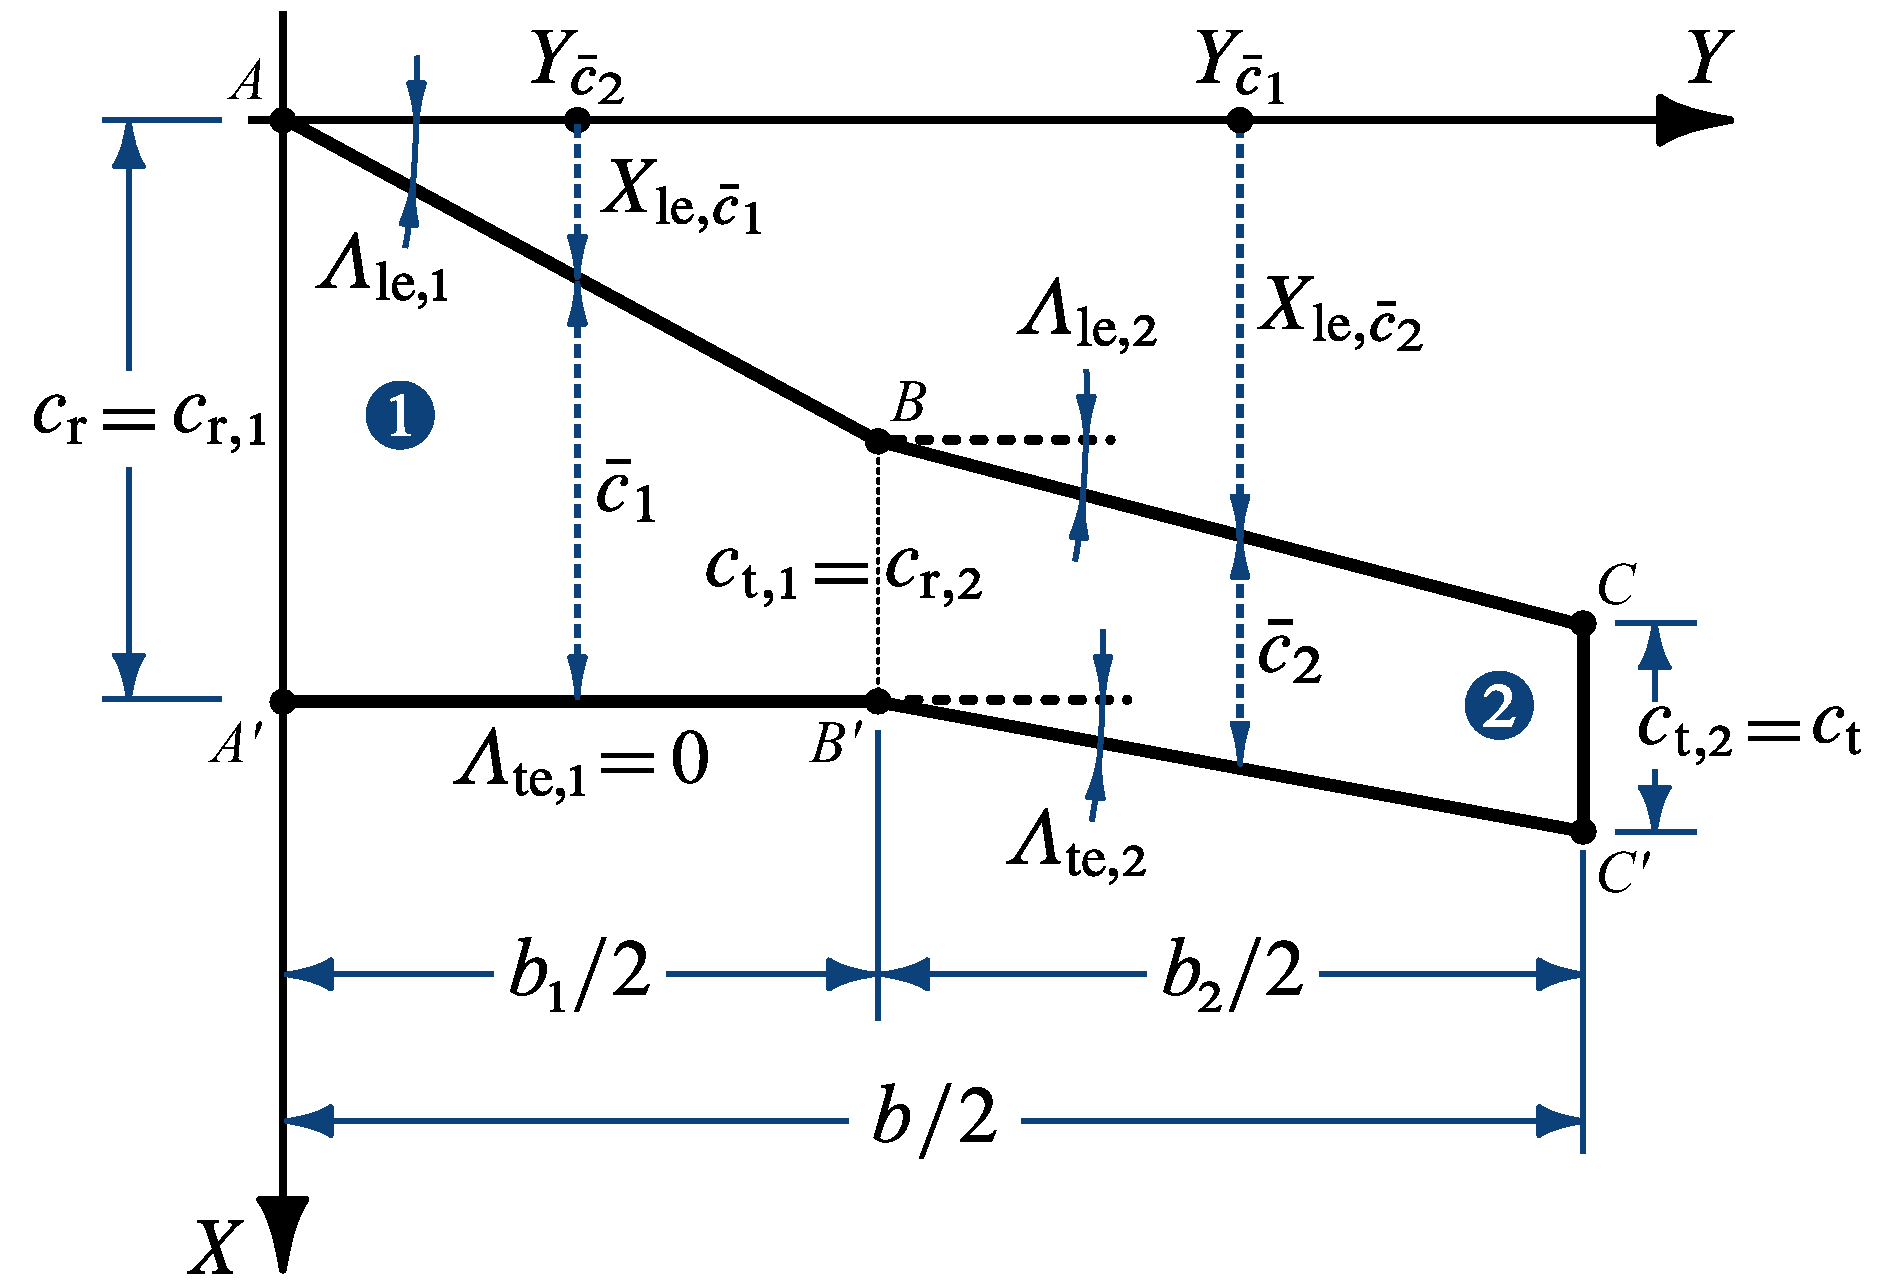
\includegraphics[width=0.72\textwidth]{images/cranked_wing.pdf}%
  \caption{\finalhyphendemerits=1000
           Ala a bordi d'attacco e d'uscita non rettilinei detta \emph{cranked wing}.}
  \label{fig:Cranked:Wing:Planform:Defs}%
\end%
    %{figure}%
    {SCfigure}%
%
%\EnlargedFigure% needs two latex passes
%    {t}% #1: t, b, p
%    {images/airfoil_geometry}% #2: the image file included by \includegraphics
%    {width=1.0\textwidth}% #3: option list to pass to \includegraphics, e.g. width=\linewidth,rotate=0
%    {\finalhyphendemerits=1000
%      Alcune caratteristiche geometriche di un profilo alare.}% #4: the caption text
%    {fig:Aero:Profilo:Geometria}% #5: the label
%\EnlargedFigureX% needs two latex passes
%  {t}% #1: t, b, p
%  {%
%    \makebox[\textwidth][c]{%
%    \includegraphics%
%      %[width=0.52\textwidth]%
%      % [height=5.5cm]%
%      [width=0.485\textwidth]%
%      {images/airfoil_Re_effect_polar.pdf}%
%    %\rule{8mm}{0pt}% <-- SPACER
%    \hfill
%    \raisebox{-0.6mm}[0pt][0pt]{%
%    \includegraphics%
%      %[width=0.52\textwidth]%
%      % [height=5.5cm]%
%      [width=0.485\textwidth]%
%      {images/airfoil_Re_effect_alpha_Cl.pdf}
%    }% end-of-raisebox
%    }% end-of-makebox
%  }% #2: the image file included by \includegraphics
%  {\finalhyphendemerits=1000
%    Influenza del numero di Reynolds, $\Reynolds_{\infty}=V_{\!\infty}c/\nu_{\infty}$,
%           sulla polare e sulla curva di portanza di un profilo NACA 64-212.%
%  }% #3: the caption text
%  {fig:Airfoil:Reynolds:Effects}%% #4: the label
%
%-----------------------------------------------------------------------------------------------
%
\def\mySpanWingMT{10.600000}
\def\mySpanWingIMT{6.360000}
\def\mySpanWingIIMT{4.240000}
\def\myChordRootWingMT{1.440000}
\def\myChordRootWingIMT{1.440000}
\def\myChordRootWingIIMT{1.440000}
\def\myChordTipWingMT{0.860000}
\def\myChordTipWingIMT{1.440000}
\def\myChordTipWingIIMT{0.860000}
\def\mySweepLEWingIIDEG{0.000000}
\def\myCoeffAChordWingI{0.000000}
\def\myCoeffBChordWingIMT{1.440000}
\def\myCoeffAChordWingII{-0.273585}
\def\myCoeffBChordWingIIMT{1.440000}
\def\myAlphaZeroLiftRootWingIDEG{-2.500000}
\def\myAlphaZeroLiftTipWingIDEG{-2.500000}
\def\myAlphaZeroLiftRootWingIRAD{-0.043633}
\def\myAlphaZeroLiftTipWingIRAD{-0.043633}
\def\myAlphaZeroLiftRootWingIIDEG{-2.500000}
\def\myAlphaZeroLiftTipWingIIDEG{-1.000000}
\def\myAlphaZeroLiftRootWingIIRAD{-0.043633}
\def\myAlphaZeroLiftTipWingIIRAD{-0.017453}
\def\myTaperRatioWingI{1.000000}
\def\myTaperRatioWingII{0.597222}
\def\myTwistWingIDEG{0.000000}
\def\myTwistWingIRAD{0.000000}
\def\myTwistWingIIDEG{-3.000000}
\def\myTwistWingIIRAD{-0.052360}
\def\myAreaWingIMTsquared{9.158400}
\def\myAreaWingIIMTsquared{4.876000}
\def\myAreaWingMTsquared{14.034400}
\def\myCoeffAAeroTwistWingIRADMT{0.000000}
\def\myCoeffBAeroTwistWingIRAD{-0.043633}
\def\myCoeffAAeroTwistWingIIRADMT{0.012349}
\def\myCoeffBAeroTwistWingIIRAD{-0.043633}
\def\myCoeffATwistWingIRADMT{0.000000}
\def\myCoeffATwistWingIIRADMT{-0.024698}
\def\myCoeffBTwistWingIRAD{0.000000}
\def\myCoeffBTwistWingIIRAD{0.000000}
\def\myAlphaZeroLiftWingIRAD{-0.028653}
\def\myAlphaZeroLiftWingIDEG{-1.641680}
\def\myAlphaZeroLiftWingIIRAD{0.008329}
\def\myAlphaZeroLiftWingIIDEG{0.477233}
\def\myAlphaZeroLiftWingRAD{-0.020323}
\def\myAlphaZeroLiftWingDEG{-1.164447}

%
\begin{myExampleX}{Caratteristiche geometriche di una cranked wing}{\ding{46}}% \ \Keyboard\ %
\label{example:Wing:Basic:B}
%
\noindent
Un'ala finita ha i bordi d'attacco e d'uscita corrispondenti a due spezzate.
In particolare, la forma in pianta della semiala destra è l'unione di due pannelli
etichettati come ``pannello~1'' (pannello interno) e ``pannello~2'' (pannello esterno), 
ed è rappresentata schematicamente nella figura~\vref{fig:Cranked:Wing:Planform:Defs}.
Questo tipo di forma in pianta è detto anche \emph{cranked wing}.

L'apertura totale è $b=\SI[round-precision=1]{\mySpanWingMT}{\metre}$,
il pannello interno ha estensione
$\frac{1}{2}b_1=\calcSI[round-precision=2,fixed-exponent=0,scientific-notation=fixed]{0.5*\mySpanWingIMT}{\metre}$,
il pannello esterno ha estensione
$\frac{1}{2}b_2=\frac{1}{2}b-\frac{1}{2}b_1
=\calcSI[round-precision=2,fixed-exponent=0,scientific-notation=fixed]{0.5*\mySpanWingIIMT}{\metre}$.
Le corde di radice e d'estremità sono
$c_\mathrm{r}=c_{\mathrm{r},1}=\SI[round-precision=2]{\myChordRootWingMT}{\metre}$ e
$c_\mathrm{t}=c_{\mathrm{t},2}=\SI[round-precision=2]{\myChordTipWingMT}{\metre}$.
Il bordo d'attacco è una linea spezzata in corrispondenza del punto $B$
e il bordo d'uscita è spezzato in corrispondenza del punto $B'$.
Entrambi hanno coordinata 
$Y_B=Y_{B'}=\frac{1}{2}b_1=\calcSI[round-precision=2,fixed-exponent=0,scientific-notation=fixed]{0.5*\mySpanWingIMT}{\metre}$.
La sezione alare $BB'$ ha corda
$c_{\mathrm{t},1}=c_{\mathrm{r},2}=\SI[round-precision=2]{\myChordRootWingIIMT}{\metre}$.
Gli angoli di freccia dei bordi d'attacco di ciascun pannello sono 
$\Lambda_\mathrm{le,1}=\SI[round-precision=1]{\mySweepLEWingIDEG}{\deg}$
e $\Lambda_\mathrm{le,2}=\SI[round-precision=1]{\mySweepLEWingIIDEG}{\deg}$.

Per l'ala \emph{cranked} assegnata si vogliono calcolare le seguenti grandezze:

\noindent
\adjustbox{center=\textwidth}{%
$S$\,, $\AR$\,, $\bar{c}$\,, $X_{\mathrm{le},\bar{c}}$\,, $Y_{\bar{c}}$
}% \,, $Y_{\bar{c}}$

\medskip
La legge delle corde di questa forma in pianta è la seguente funzione lineare a tratti:
\[
c(Y)=
\ccases{
%\left\{
%\begin{array}{cl}
c_1(Y) = A_{c,1} \, Y + B_{c,1} & \text{per }\makebox[3em][r]{$0$}     \le Y \le \frac{1}{2}b_1
\\[4pt]
c_2(Y) = A_{c,2} \, \bigg(Y-\dfrac{b_1}{2}\bigg) + B_{c,2} & \text{per }\makebox[3em][r]{$\frac{1}{2}b_1$}< Y \le \frac{1}{2}b
%\end{array}
%\right.
}
\]
i cui coefficienti si calcolano imponendo $c_1(0)=c_{\mathrm{r},1}$,
$c_1(\frac{1}{2}b_1)=c_{\mathrm{t},1}$, $c_2(\frac{1}{2}b_1)=c_{\mathrm{r},2}$, $c_2(\frac{1}{2}b)=c_{\mathrm{t},2}$.
Per i dati assegnati si ha
\[
A_{c,1}
  = \frac{c_{\mathrm{t},1} - c_{\mathrm{r},1}}{b_1/2}
  = 
    2 \frac{
      \SI[round-precision=2]{\myChordTipWingIMT}{\metre} - \SI[round-precision=2]{\myChordRootWingIMT}{\metre}
    }{
      \SI[round-precision=2]{\mySpanWingIMT}{\metre}
    }
  = \mathunderline{mydarkblue}{ \SI[round-precision=3]{\myCoeffAChordWingI}{} }
\]
\[
B_{c,1}
  = c_{\mathrm{r},1}
  = \mathunderline{mydarkblue}{ \SI[round-precision=2]{\myCoeffBChordWingIMT}{\metre} }
\]
\[
A_{c,2}
  = \frac{c_{\mathrm{t},2} - c_{\mathrm{r},2}}{b_2/2}
  = 
    2 \frac{
      \SI[round-precision=2]{\myChordTipWingIIMT}{\metre} - \SI[round-precision=2]{\myChordRootWingIIMT}{\metre}
    }{
      \SI[round-precision=2]{\mySpanWingIIMT}{\metre}
    }
  = \mathunderline{mydarkblue}{ \SI[round-precision=3]{\myCoeffAChordWingII}{} }
\]
\[
B_{c,2}
  = c_{\mathrm{r},2}
  = \mathunderline{mydarkblue}{ \SI[round-precision=2]{\myCoeffBChordWingIIMT}{\metre} }
\]
dunque
\[
c(Y)=
\ccases{
%\left\{
%\begin{array}{cl}
c_1(Y) = 
  \SI[round-precision=3]{\myCoeffAChordWingI}{} \, Y 
    + \SI[round-precision=2]{\myCoeffBChordWingIIMT}{\metre} 
  & \text{per }
    \makebox[3.5em][r]{$\SI[round-precision=0]{0}{\metre}$} 
      \le Y \le 
      \calcSI[round-precision=2,fixed-exponent=0,scientific-notation=fixed]{0.5*\mySpanWingIMT}{\metre}
\\[4pt]
c_2(Y) 
  = \SI[round-precision=3]{\myCoeffAChordWingII}{} \, 
    \big(
      Y
      - \calcSI[round-precision=2,fixed-exponent=0,scientific-notation=fixed]{0.5*\mySpanWingIMT}{\metre}
    \big)
    + \SI[round-precision=2]{\myCoeffBChordWingIIMT}{\metre} 
  & \text{per }
    \makebox[3.5em][r]{%
      $\calcSI[round-precision=2,fixed-exponent=0,scientific-notation=fixed]{0.5*\mySpanWingIMT}{\metre}$
    }% end-of-makebox
      < Y 
      \le \calcSI[round-precision=2,fixed-exponent=0,scientific-notation=fixed]{0.5*\mySpanWingMT}{\metre}
%\end{array}
%\right.
}
\]

Relativamente alla porzione alare interna, il rapporto di rastremazione è
\[
\lambda_1
  =\frac{c_{\mathrm{t},1}}{c_{\mathrm{r},1}}
  =\frac{\SI[round-precision=2]{\myChordTipWingIMT}{\metre}}{\SI[round-precision=2]{\myChordRootWingIMT}{\metre}}
  =\mathunderline{mydarkblue}{ \SI[round-precision=2]{\myTaperRatioWingI}{} }
\]
la superficie è
\[
\begin{split}
S_1 & {}= \frac{b_1}{2} \, c_{\mathrm{r},1} \, \big( 1 + \lambda_1 \big) \\
  & {}=
    \num{0.5} \cdot \SI[round-precision=1]{\mySpanWingIMT}{\metre}
      \cdot \SI[round-precision=2]{\myChordRootWingIMT}{\metre}
      \cdot \big( 1 + \SI[round-precision=2]{\myTaperRatioWingI}{} \big) 
    = \mathunderline{mydarkblue}{ \SI[round-precision=1]{\myAreaWingIMTsquared}{\metre^2} }
\end{split}
\]
e l'allungamento corrispondente è
\[
\AR_1 
  = \frac{b_1^2}{S_1}
  = \frac{\big(\SI[round-precision=1]{\mySpanWingIMT}{\metre}\big)^2}{\SI[round-precision=1]{\myAreaWingIMTsquared}{\metre^2}}
  = \mathunderline{mydarkblue}{ \num[round-precision=2]{\myAspectRatioWingI} }
\]
%
Dunque la corda media aerodinamica del pannello interno è
\[
\begin{split}
\bar{c}_1 & {}= \frac{2}{3} \, c_{\mathrm{r},1} \, \frac{1+\lambda_1 + \lambda_1^2}{1+\lambda_1} \\
  & {}=
    \num{0.667} \cdot \SI[round-precision=2]{\myChordRootWingIMT}{\metre}
      \cdot 
        \frac{
          1 + \SI[round-precision=2]{\myTaperRatioWingI}{} + \SI[round-precision=2]{\myTaperRatioWingI}{}^2
        }{
          1 + \SI[round-precision=2]{\myTaperRatioWingI}{}
        }
    = \mathunderline{mydarkblue}{ \SI[round-precision=2]{\myMACWingIMT}{\metre} }
\end{split}
\]

La distanza longitudinale del bordo d'attacco della corda media aerodinamica del pannello~1 dal
bordo d'attacco della corda di radice è
\[
\begin{split}
X_{\mathrm{le},\bar{c}_1} 
  & {}=
    \frac{b_1}{6} \, \frac{1+2\lambda_1}{1+\lambda_1} \tan\Lambda_\mathrm{le,1} \\[3pt]
  & {}=
    \frac{\SI[round-precision=1]{\mySpanWingIMT}{\metre}}{6}
      \cdot 
      \frac{
        1 + 2\cdot\SI[round-precision=2]{\myTaperRatioWingI}{}
      }{
        1 + \SI[round-precision=2]{\myTaperRatioWingI}{}
      }
      \cdot \tan \big( \SI[round-precision=3]{\mySweepLEWingIRAD}{\radian} \big)
    = \mathunderline{mydarkblue}{ \SI[round-precision=2]{\myXMACLEToApexWingIMT}{\metre} }
\end{split}
\]

La stazione lungo l'apertura corrispondente alla corda $\bar{c}_1$ è
\[
\begin{split}
Y_{\bar{c}_1} 
  & {}=
    \frac{b_1}{6} \, \frac{1+2\lambda_1}{1+\lambda_1} \\[3pt]
  & {}=
    \frac{\SI[round-precision=1]{\mySpanWingIMT}{\metre}}{6}
      \cdot 
      \frac{
        1 + 2\cdot\SI[round-precision=2]{\myTaperRatioWingI}{}
      }{
        1 + \SI[round-precision=2]{\myTaperRatioWingI}{}
      }
    = \mathunderline{mydarkblue}{ \SI[round-precision=2]{\myYMACWingIMT}{\metre} }
\end{split}
\]
In altri termini, $Y_{\bar{c}_1}$ è la distanza dal piano di mezzeria tale che
$c_1(Y_{\bar{c}_1})=\bar{c}_1$. A tale stazione lungo l'apertura corrisponde un profilo
alare il cui bordo d'attacco ha ascissa $X_{\mathrm{le},\bar{c}_1}$.


Relativamente alla porzione alare esterna, come se questa fosse isolata, 
il rapporto di rastremazione è
\[
\lambda_2
  =\frac{c_{\mathrm{t},2}}{c_{\mathrm{r},2}}
  =\frac{\SI[round-precision=2]{\myChordTipWingIIMT}{\metre}}{\SI[round-precision=2]{\myChordRootWingIIMT}{\metre}}
  =\mathunderline{mydarkblue}{ \SI[round-precision=2]{\myTaperRatioWingII}{} }
\]
la superficie è
\[
\begin{split}
S_2 & {}= \frac{b_2}{2} \, c_{\mathrm{r},2} \, \big( 1 + \lambda_2 \big) \\
  & {}=
    \num{0.5} \cdot \SI[round-precision=1]{\mySpanWingIIMT}{\metre}
      \cdot \SI[round-precision=2]{\myChordRootWingIIMT}{\metre}
      \cdot \big( 1 + \SI[round-precision=2]{\myTaperRatioWingII}{} \big) 
    = \mathunderline{mydarkblue}{ \SI[round-precision=1]{\myAreaWingIIMTsquared}{\metre^2} }
\end{split}
\]
e l'allungamento corrispondente è
\[
\AR_2 
  = \frac{b_2^2}{S_2}
  = \frac{\big(\SI[round-precision=1]{\mySpanWingIIMT}{\metre}\big)^2}{\SI[round-precision=1]{\myAreaWingIIMTsquared}{\metre^2}}
  = \mathunderline{mydarkblue}{ \num[round-precision=2]{\myAspectRatioWingII} }
\]
%
La corda media aerodinamica del pannello esterno è
\[
\begin{split}
\bar{c}_2 & {}= \frac{2}{3} \, c_{\mathrm{r},2} \, \frac{1+\lambda_2 + \lambda_2^2}{1+\lambda_2} \\
  & {}=
    \num{0.667} \cdot \SI[round-precision=2]{\myChordRootWingIIMT}{\metre}
      \cdot 
        \frac{
          1 + \SI[round-precision=2]{\myTaperRatioWingII}{} + \SI[round-precision=2]{\myTaperRatioWingII}{}^2
        }{
          1 + \SI[round-precision=2]{\myTaperRatioWingII}{}
        }
    = \mathunderline{mydarkblue}{ \SI[round-precision=2]{\myMACWingIIMT}{\metre} }
\end{split}
\]
%
La distanza longitudinale del bordo d'attacco della corda media aerodinamica del pannello~2 dal
punto $B$ è
\[
\begin{split}
X_{\mathrm{le},\bar{c}_2} - X_B
  & {}=
    \frac{b_2}{6} \, \frac{1+2\lambda_2}{1+\lambda_2} \tan\Lambda_\mathrm{le,2} \\[3pt]
  & {}=
    \frac{\SI[round-precision=1]{\mySpanWingIIMT}{\metre}}{6}
      \cdot 
      \frac{
        1 + 2\cdot\SI[round-precision=2]{\myTaperRatioWingII}{}
      }{
        1 + \SI[round-precision=2]{\myTaperRatioWingII}{}
      }
      \cdot \tan \big( \SI[round-precision=3]{\mySweepLEWingIIRAD}{\radian} \big)
    = \mathunderline{mydarkblue}{ \SI[round-precision=2]{\myXMACLEToApexWingIIMT}{\metre} }
\end{split}
\]
%
Questa distanza è quella che si calcolerebbe se l'ala coincidesse con il pannello esterno
cioè se $B$ fosse il bordo d'attacco della corda di radice.
Quindi l'ascissa $X_{\mathrm{le},\bar{c}_2}$ è
\[
\begin{split}
X_{\mathrm{le},\bar{c}_2} & {}= X_B + \SI[round-precision=2]{\myXMACLEToApexWingIIMT}{\metre}
  = \frac{b_1}{2} \tan \Lambda_{\mathrm{le},1} + \SI[round-precision=2]{\myXMACLEToApexWingIIMT}{\metre}
\\
  & {}= \calcSI[round-precision=2,fixed-exponent=0,scientific-notation=fixed]{
          0.5 * \mySpanWingIMT
        }{\metre}
       \cdot \tan( \SI[round-precision=3]{\mySweepLEWingIRAD}{\radian} )
      + \SI[round-precision=2]{\myXMACLEToApexWingIIMT}{\metre}
    = \calcSI[round-precision=2,fixed-exponent=0,scientific-notation=fixed]{
          0.5 * \mySpanWingIMT * tan( \mySweepLEWingIRAD )
        }{\metre}
      + \SI[round-precision=2]{\myXMACLEToApexWingIIMT}{\metre}
    = \mathunderline{mydarkblue}{ 
      \calcSI[round-precision=2,fixed-exponent=0,scientific-notation=fixed]{
          0.5 * \mySpanWingIMT * tan( \mySweepLEWingIRAD )
          + \myXMACLEToApexWingIIMT
      }{\metre}
    }
\end{split}
\]

La stazione lungo l'apertura alare corrispondente alla corda $\bar{c}_2$ è
\[
\begin{split}
Y_{\bar{c}_2} 
  & {}=
    \frac{b_1}{2} + 
    \frac{b_2}{6} \, \frac{1+2\lambda_2}{1+\lambda_2} \\[3pt]
  & {}=
    \calcSI[round-precision=2]{0.5*\mySpanWingIMT}{\metre} +
    \frac{\SI[round-precision=1]{\mySpanWingIIMT}{\metre}}{6}
      \cdot 
      \frac{
        1 + 2\cdot\SI[round-precision=2]{\myTaperRatioWingII}{}
      }{
        1 + \SI[round-precision=2]{\myTaperRatioWingII}{}
      }
    = \mathunderline{mydarkblue}{
      \calcSI[round-precision=2]{0.5*\mySpanWingIMT}{\metre} +
      \SI[round-precision=2]{\myYMACWingIIMT}{\metre} 
    }
    = \mathunderline{mydarkblue}{
      \calcSI[round-precision=2,fixed-exponent=0,scientific-notation=fixed]{0.5*\mySpanWingIMT + \myYMACWingIIMT}{\metre}
    }
\end{split}
\]
%
Questa è la effettiva distanza dal piano di simmetria dell'ala della stazione alare nel pannello
esterno di corda pari a $\bar{c}_2$.

La forma in pianta assegnata ha una superficie complessiva pari a
\[
S = S_1 + S_2
  = \SI[round-precision=1]{\myAreaWingIMTsquared}{\metre^2}
    = \mathunderline{mydarkblue}{
      \SI[round-precision=1]{\myAreaWingCrankedMTsquared}{\metre^2}
    }
\]
e un allungamento
\[
\AR = \frac{b^2}{S} 
    = \frac{
        \big( \SI[round-precision=2]{\mySpanWingMT}{\meter} \big)^2
      }{
        \SI[round-precision=1]{\myAreaWingCrankedMTsquared}{\metre^2}
      }
    = \mathunderline{mydarkblue}{
      \SI[round-precision=2]{\myAspectRatioWingCranked}{}
    }
\]

Dalla formula di calcolo generale della corda media aerodinamica
scritta per un'ala \emph{cranked} a due pannelli
\[
\bar{c} 
  = \frac{1}{S} \int_0^{b/2} c^2(Y) \diff{Y} 
  = \frac{1}{S} \int_0^{b_1/2} c_1^2(Y) \diff{Y} 
    + \frac{1}{S} \int_{b_1/2}^{b/2} c_2^2(Y) \diff{Y}
\]
essendo i due integrali a secondo membro pari a $S_1 \, \bar{c}_1$ e $S_2 \, \bar{c}_2$, rispettivamente,
si ha che la $\bar{c}$ dell'ala assegnata è data dalla seguente media pesata:
\[
\bar{c} = \frac{S_1 \, \bar{c}_1 + S_2 \, \bar{c}_2} {S_1 + S_2}
  =
  \frac{\SI[round-precision=1]{\myAreaWingIMTsquared}{\metre^2} \cdot \SI[round-precision=2]{\myMACWingIMT}{\metre} + \SI[round-precision=1]{\myAreaWingIIMTsquared}{\metre^2} \cdot \SI[round-precision=2]{\myMACWingIIMT}{\metre}}{\SI[round-precision=1]{\myAreaWingIMTsquared}{\metre^2} + \SI[round-precision=1]{\myAreaWingIIMTsquared}{\metre^2}}
    = \mathunderline{mydarkblue}{ \SI[round-precision=2]{\myMACWingCrankedMT}{\metre} }
\]

Si osserva che $\bar{c} > c_{\mathrm{t}.1}$, essendo $S_1>S_2$. Pertanto,
il valore della stazione $Y_{\bar{c}}$ va ricercato tra le coordinate $Y$ dei
profili montati lungo il pannello interno, cioè guardando la legge delle corde $c_1(Y)$.
Si ha dunque
\[
\bar{c}=A_{c,1}\,Y_{\bar{c}} + B_{c,1} \quad \Rightarrow \quad
  Y_{\bar{c}} 
    = \frac{\bar{c} - B_{c,1}}{A_{c,1}}
    = \frac{
      \SI[round-precision=2]{\myMACWingCrankedMT}{\metre} 
        - \SI[round-precision=2]{\myCoeffBChordWingIMT}{\metre}
      }{
        \SI[round-precision=3]{\myCoeffAChordWingI}{}
      }
    = \mathunderline{mydarkblue}{
      \SI[round-precision=2]{\myYYMACWingCrankedMT}{\metre}
    }
\]
Verificare, per esercizio, che quando $S_2 > S_1$ va applicata la seguente formula:
\[
Y_{\bar{c}} = \frac{b_1}{2} + \frac{\bar{c} - B_{c,2}}{A_{c,2}}
\]

Individuata tale stazione, si estrae la coordinata $X$ del bordo d'attacco 
della corda corrispondente, cioè la $X_{\mathrm{le},\bar{c}}$.
La distanza longitudinale del bordo d'attacco della corda media aerodinamica dell'ala \emph{cranked} dal
bordo d'attacco della corda di radice è in questo caso
\[
X_{\mathrm{le},\bar{c}} 
  = Y_{\bar{c}} \tan \Lambda_{\mathrm{le},1}
  = \SI[round-precision=2]{\myYYMACWingCrankedMT}{\metre}
    \cdot \tan( \SI[round-precision=3]{\mySweepLEWingIRAD}{\radian} )
  = \mathunderline{mydarkblue}{ \SI[round-precision=2]{\myXXMACLEToApexWingCrankedMT}{\metre} }
\]
Verificare, per esercizio, che quando $S_2 > S_1$ va applicata la seguente formula:
\[
X_{\mathrm{le},\bar{c}} 
  = \frac{b_1}{2} \tan \Lambda_{\mathrm{le},1}
    + \frac{\bar{c} - B_{c,2}}{A_{c,2}} \tan \Lambda_{\mathrm{le},2}
\]

La figura~\vref{fig:Cranked:Wing:Planform:Results} riporta il disegno della forma in pianta
assegnata.
Sono evidenziate le corde aerodinamiche dei singoli pannelli e la corda $\bar{c}$.
In basso nella figura è anche riportata la legge delle corde $c(Y)$.

\end{myExampleX}

%-----------------------------------------------------------------------------------------------
\begin%
  %{figure}
  {SCfigure}[1.9]%
  [t]%[H]%[!htbp]
  %\centering
  %\checkoddpage
  %\centering
    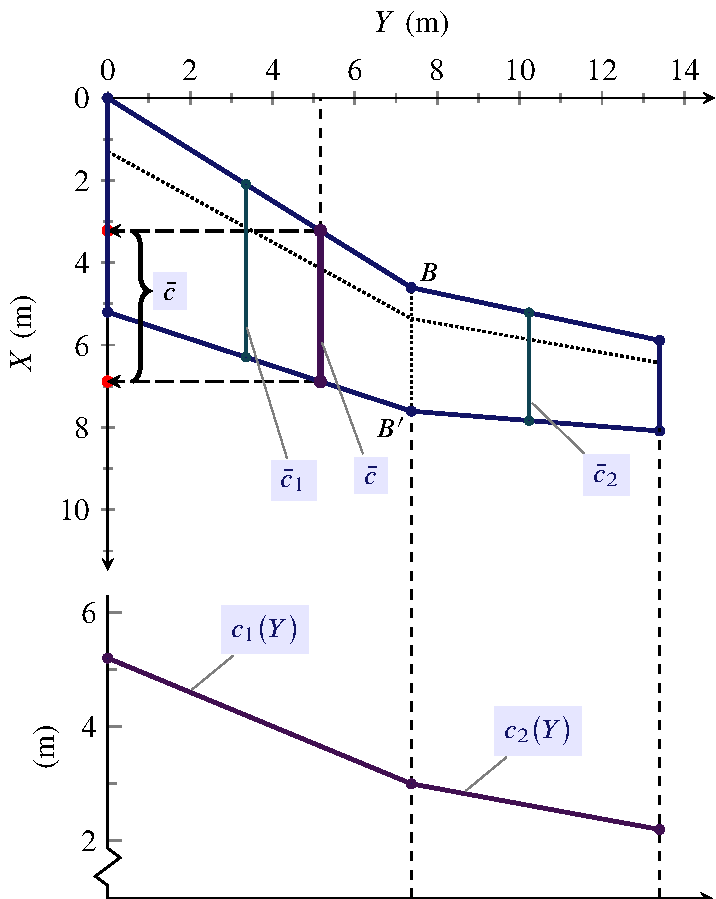
\includegraphics[width=0.78\textwidth]{exercises/wing_planform_basic_2/wing_planform_basic_2_drawing.pdf}%
  \caption{\finalhyphendemerits=1000
           Forma in pianta dell'ala \emph{cranked} assegnata nell'esempio~\ref{example:Wing:Basic:B}.
           È riportata anche la legge delle corde lineare a tratti.
  }
  \label{fig:Cranked:Wing:Planform:Results}%
\end%
    %{figure}%
    {SCfigure}%
%
%\EnlargedFigure% needs two latex passes
%    {t}% #1: t, b, p
%    {images/airfoil_geometry}% #2: the image file included by \includegraphics
%    {width=1.0\textwidth}% #3: option list to pass to \includegraphics, e.g. width=\linewidth,rotate=0
%    {\finalhyphendemerits=1000
%      Alcune caratteristiche geometriche di un profilo alare.}% #4: the caption text
%    {fig:Aero:Profilo:Geometria}% #5: the label
%\EnlargedFigureX% needs two latex passes
%  {t}% #1: t, b, p
%  {%
%    \makebox[\textwidth][c]{%
%    \includegraphics%
%      %[width=0.52\textwidth]%
%      % [height=5.5cm]%
%      [width=0.485\textwidth]%
%      {images/airfoil_Re_effect_polar.pdf}%
%    %\rule{8mm}{0pt}% <-- SPACER
%    \hfill
%    \raisebox{-0.6mm}[0pt][0pt]{%
%    \includegraphics%
%      %[width=0.52\textwidth]%
%      % [height=5.5cm]%
%      [width=0.485\textwidth]%
%      {images/airfoil_Re_effect_alpha_Cl.pdf}
%    }% end-of-raisebox
%    }% end-of-makebox
%  }% #2: the image file included by \includegraphics
%  {\finalhyphendemerits=1000
%    Influenza del numero di Reynolds, $\Reynolds_{\infty}=V_{\!\infty}c/\nu_{\infty}$,
%           sulla polare e sulla curva di portanza di un profilo NACA 64-212.%
%  }% #3: the caption text
%  {fig:Airfoil:Reynolds:Effects}%% #4: the label
%
%-----------------------------------------------------------------------------------------------
%
%--END-EXERCISE:wing_planform_basic_2
%===============================================================================================

%===============================================================================================
%--BEGIN-EXERCISE:ES:wing_planform_basic_2_A
%
%
\def\mySpanWingMT{10.600000}
\def\mySpanWingIMT{6.360000}
\def\mySpanWingIIMT{4.240000}
\def\myChordRootWingMT{1.440000}
\def\myChordRootWingIMT{1.440000}
\def\myChordRootWingIIMT{1.440000}
\def\myChordTipWingMT{0.860000}
\def\myChordTipWingIMT{1.440000}
\def\myChordTipWingIIMT{0.860000}
\def\mySweepLEWingIIDEG{0.000000}
\def\myCoeffAChordWingI{0.000000}
\def\myCoeffBChordWingIMT{1.440000}
\def\myCoeffAChordWingII{-0.273585}
\def\myCoeffBChordWingIIMT{1.440000}
\def\myAlphaZeroLiftRootWingIDEG{-2.500000}
\def\myAlphaZeroLiftTipWingIDEG{-2.500000}
\def\myAlphaZeroLiftRootWingIRAD{-0.043633}
\def\myAlphaZeroLiftTipWingIRAD{-0.043633}
\def\myAlphaZeroLiftRootWingIIDEG{-2.500000}
\def\myAlphaZeroLiftTipWingIIDEG{-1.000000}
\def\myAlphaZeroLiftRootWingIIRAD{-0.043633}
\def\myAlphaZeroLiftTipWingIIRAD{-0.017453}
\def\myTaperRatioWingI{1.000000}
\def\myTaperRatioWingII{0.597222}
\def\myTwistWingIDEG{0.000000}
\def\myTwistWingIRAD{0.000000}
\def\myTwistWingIIDEG{-3.000000}
\def\myTwistWingIIRAD{-0.052360}
\def\myAreaWingIMTsquared{9.158400}
\def\myAreaWingIIMTsquared{4.876000}
\def\myAreaWingMTsquared{14.034400}
\def\myCoeffAAeroTwistWingIRADMT{0.000000}
\def\myCoeffBAeroTwistWingIRAD{-0.043633}
\def\myCoeffAAeroTwistWingIIRADMT{0.012349}
\def\myCoeffBAeroTwistWingIIRAD{-0.043633}
\def\myCoeffATwistWingIRADMT{0.000000}
\def\myCoeffATwistWingIIRADMT{-0.024698}
\def\myCoeffBTwistWingIRAD{0.000000}
\def\myCoeffBTwistWingIIRAD{0.000000}
\def\myAlphaZeroLiftWingIRAD{-0.028653}
\def\myAlphaZeroLiftWingIDEG{-1.641680}
\def\myAlphaZeroLiftWingIIRAD{0.008329}
\def\myAlphaZeroLiftWingIIDEG{0.477233}
\def\myAlphaZeroLiftWingRAD{-0.020323}
\def\myAlphaZeroLiftWingDEG{-1.164447}

%
\begin{myExerciseX}{Corda media aerodinamica di un'ala cranked}{\ding{46}}% \ \Keyboard\ %
\label{exercise:Cranked:Wing:Planform:Basic:B}
%
\noindent

Si consideri l'ala finita la cui semiala destra ha la forma in pianta riportata
nella figura~\ref{fig:Cranked:Wing:Planform:Results:B}.
Il pannello interno ha corda costante pari a
$c_\mathrm{r}=c_{\mathrm{r},1}=\SI[round-precision=2]{\myChordRootWingIMT}{\metre}$
ed ha un'apertura 
$\frac{1}{2}b_1=\calcSI[round-precision=2,fixed-exponent=0,scientific-notation=fixed]{0.5*\mySpanWingIMT}{\metre}$.
Il pannello esterno ha corda d'estremità
$c_\mathrm{t}=c_{\mathrm{t},2}=\SI[round-precision=2]{\myChordTipWingIIMT}{\metre}$
e si estende per un'apertura 
$\frac{1}{2}b_2=\calcSI[round-precision=2,fixed-exponent=0,scientific-notation=fixed]{0.5*\mySpanWingIIMT}{\metre}$.
La semiapertura alare è 
$\frac{1}{2}b=\frac{1}{2}b_1+\frac{1}{2}b_2=\SI[round-precision=2]{\mySpanWingMT}{\metre}$.

Ricostruire la legge delle corde per $0\le Y \le \frac{1}{2}b$ e
verificare che l'ala ha una corda media aerodinamica 
$\bar{c}= \SI[round-precision=2]{\myMACWingCrankedMT}{\metre}$.
Verificare inoltre
che $X_{\mathrm{le},\bar{c}}=\SI[round-precision=0]{0}{\metre}$ 
e $Y_{\bar{c}}=\SI[round-precision=2]{\myYYMACWingCrankedMT}{\metre}$.

\end{myExerciseX}

%-----------------------------------------------------------------------------------------------
\begin%
  %{figure}
  {SCfigure}[1.9]%
  [t]%[H]%[!htbp]
  %\centering
  %\checkoddpage
  %\centering
    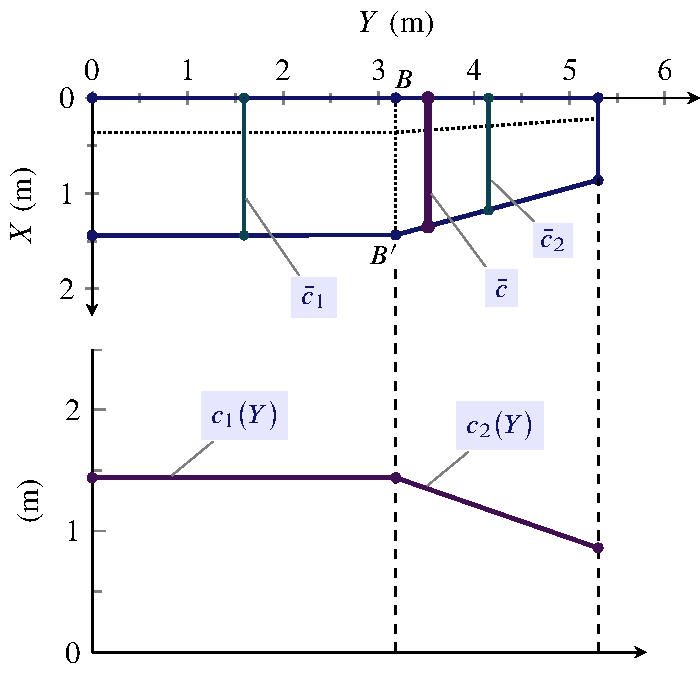
\includegraphics[width=0.68\textwidth]{exercises/wing_planform_basic_2A/wing_planform_basic_2A_drawing.pdf}%
  \caption{\finalhyphendemerits=1000
           Forma in pianta dell'ala \emph{cranked} assegnata
           nell'esercizio~\ref{exercise:Cranked:Wing:Planform:Basic:B}.
           È riportata anche la legge delle corde lineare a tratti.
  }
  \label{fig:Cranked:Wing:Planform:Results:B}%
\end%
    %{figure}%
    {SCfigure}%
%
%\EnlargedFigure% needs two latex passes
%    {t}% #1: t, b, p
%    {images/airfoil_geometry}% #2: the image file included by \includegraphics
%    {width=1.0\textwidth}% #3: option list to pass to \includegraphics, e.g. width=\linewidth,rotate=0
%    {\finalhyphendemerits=1000
%      Alcune caratteristiche geometriche di un profilo alare.}% #4: the caption text
%    {fig:Aero:Profilo:Geometria}% #5: the label
%\EnlargedFigureX% needs two latex passes
%  {t}% #1: t, b, p
%  {%
%    \makebox[\textwidth][c]{%
%    \includegraphics%
%      %[width=0.52\textwidth]%
%      % [height=5.5cm]%
%      [width=0.485\textwidth]%
%      {images/airfoil_Re_effect_polar.pdf}%
%    %\rule{8mm}{0pt}% <-- SPACER
%    \hfill
%    \raisebox{-0.6mm}[0pt][0pt]{%
%    \includegraphics%
%      %[width=0.52\textwidth]%
%      % [height=5.5cm]%
%      [width=0.485\textwidth]%
%      {images/airfoil_Re_effect_alpha_Cl.pdf}
%    }% end-of-raisebox
%    }% end-of-makebox
%  }% #2: the image file included by \includegraphics
%  {\finalhyphendemerits=1000
%    Influenza del numero di Reynolds, $\Reynolds_{\infty}=V_{\!\infty}c/\nu_{\infty}$,
%           sulla polare e sulla curva di portanza di un profilo NACA 64-212.%
%  }% #3: the caption text
%  {fig:Airfoil:Reynolds:Effects}%% #4: the label
%
%-----------------------------------------------------------------------------------------------
%
%--END-EXERCISE:ES:wing_planform_basic_2_A
%===============================================================================================

%===============================================================================================
%--BEGIN-EXERCISE:wing_planform_basic_3
%
%-----------------------------------------------------------------------------------------------
\begin%
  %{figure}
  {SCfigure}[1.9]%
  [t]%[H]%[!htbp]
  %\centering
  %\checkoddpage
  %\centering
    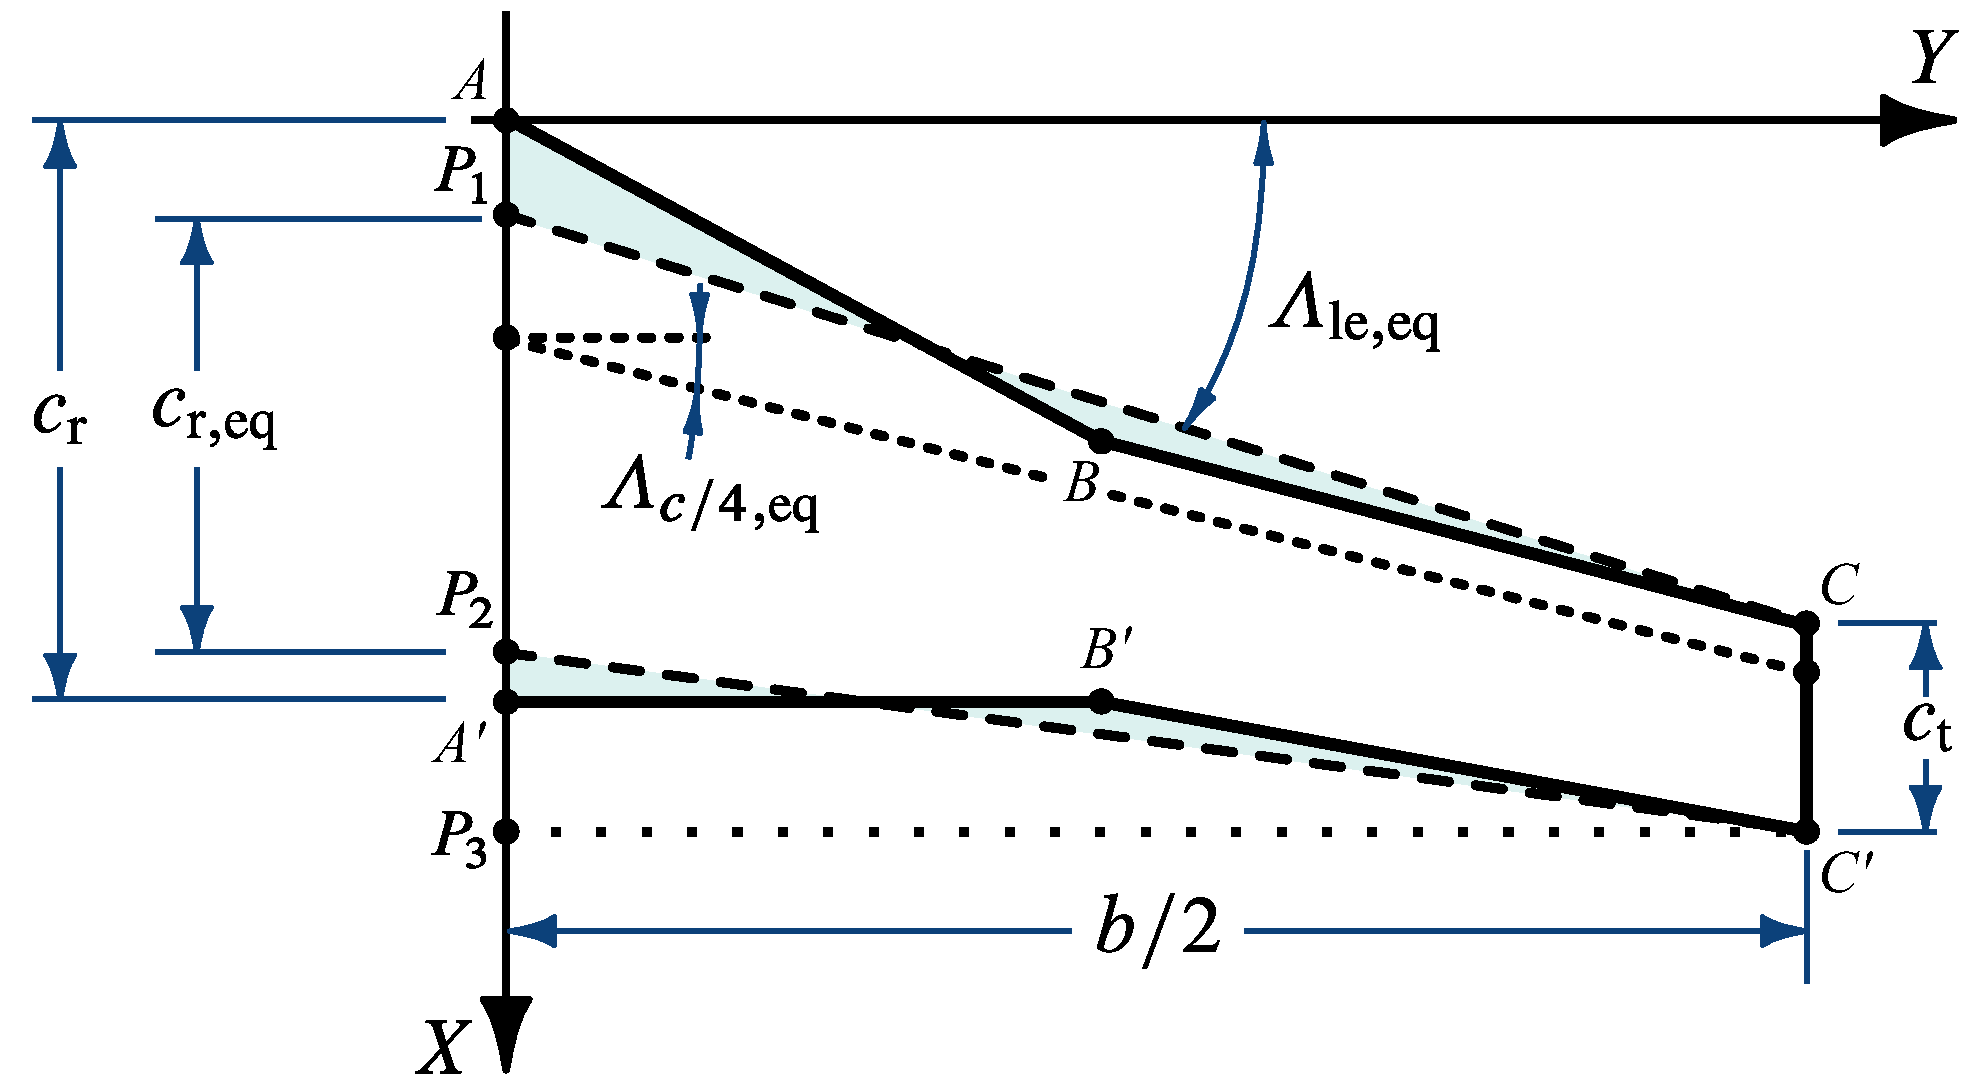
\includegraphics[width=0.78\textwidth]{images/equivalent_wing.pdf}%
  \caption{\finalhyphendemerits=1000
           Ala a bordi d'attacco e d'uscita non rettilinei ed ala equivalente a bordi dritti.}
  \label{fig:Equivalent:Wing:Planform:Defs}%
\end%
    %{figure}%
    {SCfigure}%
%
%\EnlargedFigure% needs two latex passes
%    {t}% #1: t, b, p
%    {images/airfoil_geometry}% #2: the image file included by \includegraphics
%    {width=1.0\textwidth}% #3: option list to pass to \includegraphics, e.g. width=\linewidth,rotate=0
%    {\finalhyphendemerits=1000
%      Alcune caratteristiche geometriche di un profilo alare.}% #4: the caption text
%    {fig:Aero:Profilo:Geometria}% #5: the label
%\EnlargedFigureX% needs two latex passes
%  {t}% #1: t, b, p
%  {%
%    \makebox[\textwidth][c]{%
%    \includegraphics%
%      %[width=0.52\textwidth]%
%      % [height=5.5cm]%
%      [width=0.485\textwidth]%
%      {images/airfoil_Re_effect_polar.pdf}%
%    %\rule{8mm}{0pt}% <-- SPACER
%    \hfill
%    \raisebox{-0.6mm}[0pt][0pt]{%
%    \includegraphics%
%      %[width=0.52\textwidth]%
%      % [height=5.5cm]%
%      [width=0.485\textwidth]%
%      {images/airfoil_Re_effect_alpha_Cl.pdf}
%    }% end-of-raisebox
%    }% end-of-makebox
%  }% #2: the image file included by \includegraphics
%  {\finalhyphendemerits=1000
%    Influenza del numero di Reynolds, $\Reynolds_{\infty}=V_{\!\infty}c/\nu_{\infty}$,
%           sulla polare e sulla curva di portanza di un profilo NACA 64-212.%
%  }% #3: the caption text
%  {fig:Airfoil:Reynolds:Effects}%% #4: the label
%
%-----------------------------------------------------------------------------------------------

\def\mySpanWingMT{10.600000}
\def\mySpanWingIMT{6.360000}
\def\mySpanWingIIMT{4.240000}
\def\myChordRootWingMT{1.440000}
\def\myChordRootWingIMT{1.440000}
\def\myChordRootWingIIMT{1.440000}
\def\myChordTipWingMT{0.860000}
\def\myChordTipWingIMT{1.440000}
\def\myChordTipWingIIMT{0.860000}
\def\mySweepLEWingIIDEG{0.000000}
\def\myCoeffAChordWingI{0.000000}
\def\myCoeffBChordWingIMT{1.440000}
\def\myCoeffAChordWingII{-0.273585}
\def\myCoeffBChordWingIIMT{1.440000}
\def\myAlphaZeroLiftRootWingIDEG{-2.500000}
\def\myAlphaZeroLiftTipWingIDEG{-2.500000}
\def\myAlphaZeroLiftRootWingIRAD{-0.043633}
\def\myAlphaZeroLiftTipWingIRAD{-0.043633}
\def\myAlphaZeroLiftRootWingIIDEG{-2.500000}
\def\myAlphaZeroLiftTipWingIIDEG{-1.000000}
\def\myAlphaZeroLiftRootWingIIRAD{-0.043633}
\def\myAlphaZeroLiftTipWingIIRAD{-0.017453}
\def\myTaperRatioWingI{1.000000}
\def\myTaperRatioWingII{0.597222}
\def\myTwistWingIDEG{0.000000}
\def\myTwistWingIRAD{0.000000}
\def\myTwistWingIIDEG{-3.000000}
\def\myTwistWingIIRAD{-0.052360}
\def\myAreaWingIMTsquared{9.158400}
\def\myAreaWingIIMTsquared{4.876000}
\def\myAreaWingMTsquared{14.034400}
\def\myCoeffAAeroTwistWingIRADMT{0.000000}
\def\myCoeffBAeroTwistWingIRAD{-0.043633}
\def\myCoeffAAeroTwistWingIIRADMT{0.012349}
\def\myCoeffBAeroTwistWingIIRAD{-0.043633}
\def\myCoeffATwistWingIRADMT{0.000000}
\def\myCoeffATwistWingIIRADMT{-0.024698}
\def\myCoeffBTwistWingIRAD{0.000000}
\def\myCoeffBTwistWingIIRAD{0.000000}
\def\myAlphaZeroLiftWingIRAD{-0.028653}
\def\myAlphaZeroLiftWingIDEG{-1.641680}
\def\myAlphaZeroLiftWingIIRAD{0.008329}
\def\myAlphaZeroLiftWingIIDEG{0.477233}
\def\myAlphaZeroLiftWingRAD{-0.020323}
\def\myAlphaZeroLiftWingDEG{-1.164447}

%
\begin{myExampleX}{Forma in pianta equivalente di una cranked wing}{\ding{46}}% \ \Keyboard\ %
\label{example:Wing:Basic:C}
%
\noindent
Con riferimento all'esempio~\ref{example:Wing:Basic:B} e alla 
figura~\ref{fig:Equivalent:Wing:Planform:Defs}
si vuole trovare una forma in pianta semplice,
con bordi d'attacco e d'uscita dritti, che sia equivalente
ad un'ala \emph{cranked} a due pannelli.

L'ala equivalente ha
area $S$ della forma in pianta, apertura $b$ e corda d'estremità $c_\mathrm{t}$ 
uguali a quelle dell'ala \emph{cranked}.
In particolare, dallo schema della figura~\ref{fig:Equivalent:Wing:Planform:Defs}
la posizione relativa della corda d'estremità rispetto all'apice $A$ dell'ala assegnata
è invariata. 

Per l'ala \emph{cranked} assegnata nell'esempio~\ref{example:Wing:Basic:B} si vuole conoscere:

\noindent
\adjustbox{center=\textwidth}{%
$P_1$\,, $P_2$\,, $c_{\mathrm{r,eqv}}$\,, $\lambda_{\mathrm{eqv}}$\,, $\Lambda_{\mathrm{le,eqv}}$
}% \,, $Y_{\bar{c}}$

\medskip
Le posizioni $P_1$ e $P_2$, rispettivamente, del bordo
d'attacco e del bordo d'uscita dell'ala equivalente 
vanno trovate imponendo opportunamente
le condizioni di equivalenza su enunciate.
La posizione del punto $P_1$ si calcola imponendo:
\[
\text{Area}\big(P_1 C C' P_3 P_1\big) = \text{Area}\big(A B C C' P_3 A \big)
\]
oppure, detta $C''$ la proiezione di $C$ sull'asse delle $X$, imponendo:
\[
\text{Area}\big(P_1 C C'' P_1\big) = \text{Area}\big(A B C C'' A \big)
\]
La posizione del punto $P_2$ si calcola imponendo:
\[
\text{Area}\big(P_2 C' P_3 P_2\big)=\text{Area}\big(A' B' C' P_3 A' \big)
\]

Dallo schema di riferimento, i dati del problemma permettono di calcolare
\[
Y_B = \frac{b_1}{2} = \mathunderline{mydarkblue}{
  \calcSI[round-precision=2,fixed-exponent=0,scientific-notation=fixed]{0.5*\mySpanWingIMT}{\metre}
}
\]

\[
X_B = Y_B \tan \Lambda_{\mathrm{le},1}
  = \calcSI[round-precision=2,fixed-exponent=0,scientific-notation=fixed]{0.5*\mySpanWingIMT}{\metre}
    \cdot \tan( \SI[round-precision=3]{\mySweepLEWingIRAD}{\radian} )
  = \mathunderline{mydarkblue}{
    \calcSI[round-precision=2,fixed-exponent=0,scientific-notation=fixed]{
      0.5*\mySpanWingIMT * tan(\mySweepLEWingIRAD)
    }{\metre}
  }
\]

\[
Y_C = \frac{b}{2} 
  = \mathunderline{mydarkblue}{
    \calcSI[round-precision=2,fixed-exponent=0,scientific-notation=fixed]{0.5*\mySpanWingMT}{\metre}
  }
\]

\[
X_C = X_B + \frac{b_2}{2} \tan \Lambda_{\mathrm{le},2} =
  \calcSI[round-precision=2,fixed-exponent=0,scientific-notation=fixed]{
    0.5*\mySpanWingIMT * tan(\mySweepLEWingIRAD)
  }{\metre}
  +
  \calcSI[round-precision=2,fixed-exponent=0,scientific-notation=fixed]{
    0.5*\mySpanWingIIMT
  }{\metre}
  \cdot \tan( \SI[round-precision=3]{\mySweepLEWingIIRAD}{\radian} )
  = \mathunderline{mydarkblue}{
    \calcSI[round-precision=2,fixed-exponent=0,scientific-notation=fixed]{
      0.5*\mySpanWingIMT * tan(\mySweepLEWingIRAD)
      + 0.5*\mySpanWingIIMT * tan(\mySweepLEWingIIRAD)
    }{\metre}
  }
\]

\[
Y_{C'} = Y_{C}
  = \mathunderline{mydarkblue}{
    \calcSI[round-precision=2,fixed-exponent=0,scientific-notation=fixed]{0.5*\mySpanWingMT}{\metre}
  }
\]

\[
X_{C'} = X_C + c_{\mathrm{t}}
  = \calcSI[round-precision=2,fixed-exponent=0,scientific-notation=fixed]{
    0.5*\mySpanWingIMT * tan(\mySweepLEWingIRAD)
    + 0.5*\mySpanWingIIMT * tan(\mySweepLEWingIIRAD)
  }{\metre}
  + \SI[round-precision=2]{\myChordTipWingMT}{\metre}
  = \mathunderline{mydarkblue}{
    \calcSI[round-precision=2,fixed-exponent=0,scientific-notation=fixed]{
      0.5*\mySpanWingIMT * tan(\mySweepLEWingIRAD)
      + 0.5*\mySpanWingIIMT * tan(\mySweepLEWingIIRAD)
      + \myChordTipWingMT
    }{\metre}
  }
\]

\[
Y_{B'} = Y_{B}
  = \mathunderline{mydarkblue}{
    \calcSI[round-precision=2,fixed-exponent=0,scientific-notation=fixed]{0.5*\mySpanWingIMT}{\metre}
  }
\]

\[
X_{B'} = X_{B} + c_{\mathrm{t},1}
  = \calcSI[round-precision=2,fixed-exponent=0,scientific-notation=fixed]{
    0.5*\mySpanWingIMT * tan(\mySweepLEWingIRAD)
  }{\metre}
  + \SI[round-precision=2]{\myChordTipWingIMT}{\metre}
  = \mathunderline{mydarkblue}{
    \calcSI[round-precision=2,fixed-exponent=0,scientific-notation=fixed]{
      0.5*\mySpanWingIMT * tan(\mySweepLEWingIRAD)
      + \myChordTipWingIMT
    }{\metre}
  }
\]

\[
X_{A'} = c_{\mathrm{r},1}
  = \mathunderline{mydarkblue}{
    \SI[round-precision=2]{\myChordRootWingIMT}{\metre}
  }
\]

La condizione che definisce il punto $P_1$ diventa dunque
\[
\frac{1}{2}\big( X_C - X_{P_1} \big) \, Y_C
  = \frac{1}{2} \Big[ X_C + \big( X_C - X_B \big) \Big] \, Y_B
    + \frac{1}{2}\big( X_C - X_B \big) \big( Y_C - Y_B \big)
\]
cioè un'equazione algebrica nell'incognita $X_{P_1}$. Sostituendo i valori precedentemente
calcolati, si ottiene
\[
X_{P_1}
  = \mathunderline{mydarkblue}{
    \SI[round-precision=2]{\myXEquivalentChordLEToApexWingMT}{\metre}
  }
\]

Analogamente,
la condizione che definisce il punto $P_2$ diventa
\[
\frac{1}{2}\big( X_{C'} - X_{P_2} \big) \, Y_{C'}
  = \frac{1}{2} \Big[ \big( X_{C'} - X_{A'} \big) + \big( X_{C'} - X_{B'} \big) \Big] \, Y_{B'}
    + \frac{1}{2}\big( X_{C'} - X_{B'} \big) \big( Y_{C'} - Y_{B'} \big)
\]
cioè un'equazione algebrica nell'incognita $X_{P_2}$. Sostituendo i valori precedentemente
calcolati, si ottiene
\[
X_{P_2}
  = \mathunderline{mydarkblue}{
    \SI[round-precision=2]{\myXEquivalentChordTEToApexWingMT}{\metre}
  }
\]

I risultati precedenti permettono di calcolare la corda di radice dell'ala equivalente
\[
c_{\mathrm{r,eqv}} = X_{P_2} - X_{P_1}
  = \SI[round-precision=2]{\myXEquivalentChordTEToApexWingMT}{\metre}
    - \SI[round-precision=2]{\myXEquivalentChordLEToApexWingMT}{\metre}
  = \mathunderline{mydarkblue}{
    \SI[round-precision=2]{\myRootChordWingLongitudinalPlaneMT}{\metre}
  }
\]
Da questo dato è possibile ottenere il rapporto di rastremazione
\[
\lambda_{\mathrm{eqv}} = \frac{c_\mathrm{t}}{c_{\mathrm{r,eqv}}}
  = \frac{
      \SI[round-precision=2]{\myChordTipWingMT}{\metre}
    }{ 
      \SI[round-precision=2]{\myRootChordWingLongitudinalPlaneMT}{\metre}
    }
  = \mathunderline{mydarkblue}{
    \SI[round-precision=2]{\myEquivalentTaperRatioWing}{}
  }
\]
valore diverso da quello dell'ala originale 
$\lambda = c_\mathrm{t}/c_{\mathrm{r},1}=\SI[round-precision=2]{\myTaperRatioWing}{}$.

Trovare una forma in pianta semplice che sia equivalente ad un'ala di forma in pianta
a bordi spezzati risulta utile quando si devono usare metodi semiempirici per la valutazione
dei coefficienti aerodinamici di un velivolo. In alcuni casi tali metodi richiedono dei dati
di ingresso relativi a un'ala semplice ---
ad esempio l'angolo di freccia $\Lambda_{\mathrm{le}}$ oppure $\Lambda_{c/4}$ ---
e, disponendo di un'ala \emph{cranked}, è opportuno individuare gli angoli
$\Lambda_{\mathrm{le,eqv}}$ o $\Lambda_{c/4,\mathrm{eqv}}$
dell'ala equivalente prima di usarli per il calcolo richiesto.

L'angolo di freccia del bordo d'attacco dell'ala equivalente si calcola come
segue:
\[
\tan \Lambda_{\mathrm{le,eqv}} = \frac{X_C - X_{P_1}}{b/2}
  = \frac{
    \calcSI[round-precision=2,fixed-exponent=0,scientific-notation=fixed]{
      0.5*\mySpanWingIMT * tan(\mySweepLEWingIRAD)
      + 0.5*\mySpanWingIIMT * tan(\mySweepLEWingIIRAD)
    }{\metre}
      - \SI[round-precision=2]{\myXEquivalentChordLEToApexWingMT}{\metre}
  }{ 
    \calcSI[round-precision=2,fixed-exponent=0,scientific-notation=fixed]{0.5*\mySpanWingMT}{\metre}
  }
\quad \Rightarrow \quad
\Lambda_{\mathrm{le,eqv}}
  = \mathunderline{mydarkblue}{
    \SI[round-precision=3]{\myEquivalentSweepLEWingRAD}{\radian}
  }
  = \mathunderline{mydarkblue}{
    \SI[round-precision=1]{\myEquivalentSweepLEWingDEG}{\deg}
  }
\]
Per esercizio, verificare che
\[
\Lambda_{c/4,\mathrm{eqv}}
  = \mathunderline{mydarkblue}{
    \SI[round-precision=3]{\myEquivalentSweepQuarterChordWingRAD}{\radian}
  }
  = \mathunderline{mydarkblue}{
    \SI[round-precision=1]{\myEquivalentSweepQuarterChordWingDEG}{\deg}
  }
\]
\[
\Lambda_{c/2,\mathrm{eqv}}
  = \mathunderline{mydarkblue}{
    \SI[round-precision=3]{\myEquivalentSweepHalfChordWingRAD}{\radian}
  }
  = \mathunderline{mydarkblue}{
    \SI[round-precision=1]{\myEquivalentSweepHalfChordWingDEG}{\deg}
  }
\]
\[
\Lambda_{\mathrm{te,eqv}}
  = \mathunderline{mydarkblue}{
    \SI[round-precision=3]{\myEquivalentSweepTEWingRAD}{\radian}
  }
  = \mathunderline{mydarkblue}{
    \SI[round-precision=1]{\myEquivalentSweepTEWingDEG}{\deg}
  }
\]

La figura~\ref{fig:Equivalent:Wing:Planform:Results} riporta la forma in pianta
assegnata e quella della forma in pianta equivalente.

\end{myExampleX}

%-----------------------------------------------------------------------------------------------
\begin%
  %{figure}
  {SCfigure}[1.9]%
  [t]%[H]%[!htbp]
  %\centering
  %\checkoddpage
  %\centering
    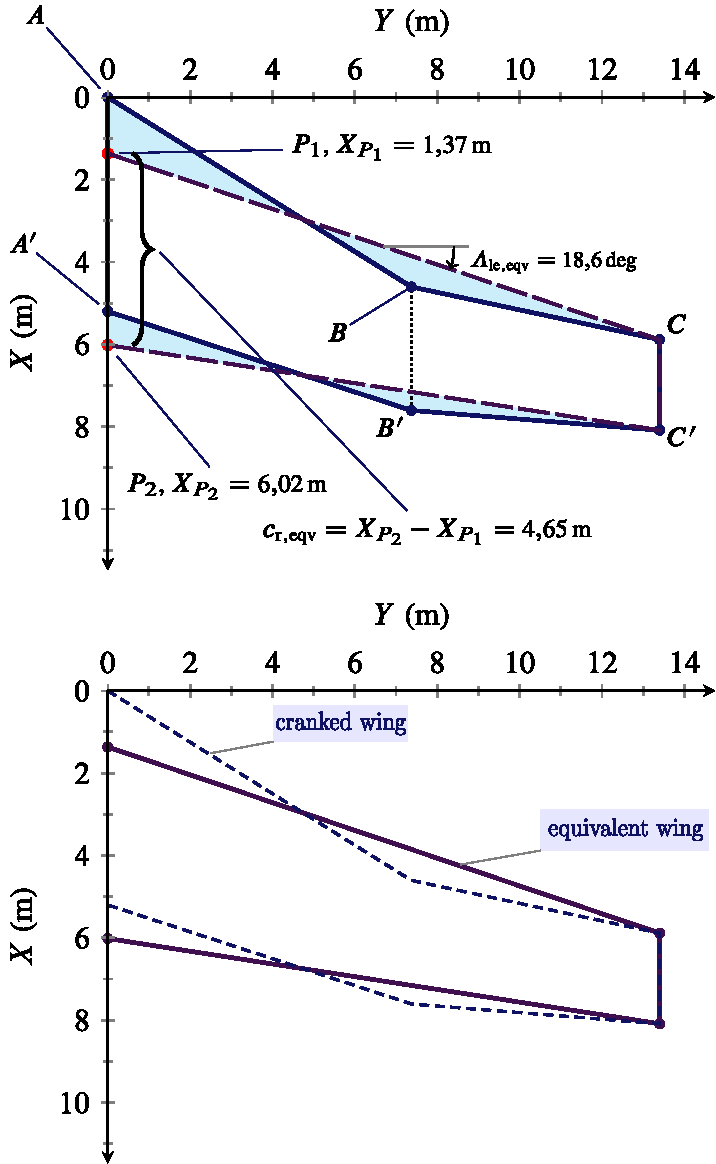
\includegraphics[width=0.68\textwidth]{exercises/wing_planform_basic_3/wing_planform_basic_3_drawing.pdf}%
  \caption{\finalhyphendemerits=1000
           Ala \emph{cranked} assegnata negli esempi~\ref{example:Wing:Basic:B} e~\ref{example:Wing:Basic:C}
           e forma in pianta equivalente.
  }
  \label{fig:Equivalent:Wing:Planform:Results}%
\end%
    %{figure}%
    {SCfigure}%
%
%\EnlargedFigure% needs two latex passes
%    {t}% #1: t, b, p
%    {images/airfoil_geometry}% #2: the image file included by \includegraphics
%    {width=1.0\textwidth}% #3: option list to pass to \includegraphics, e.g. width=\linewidth,rotate=0
%    {\finalhyphendemerits=1000
%      Alcune caratteristiche geometriche di un profilo alare.}% #4: the caption text
%    {fig:Aero:Profilo:Geometria}% #5: the label
%\EnlargedFigureX% needs two latex passes
%  {t}% #1: t, b, p
%  {%
%    \makebox[\textwidth][c]{%
%    \includegraphics%
%      %[width=0.52\textwidth]%
%      % [height=5.5cm]%
%      [width=0.485\textwidth]%
%      {images/airfoil_Re_effect_polar.pdf}%
%    %\rule{8mm}{0pt}% <-- SPACER
%    \hfill
%    \raisebox{-0.6mm}[0pt][0pt]{%
%    \includegraphics%
%      %[width=0.52\textwidth]%
%      % [height=5.5cm]%
%      [width=0.485\textwidth]%
%      {images/airfoil_Re_effect_alpha_Cl.pdf}
%    }% end-of-raisebox
%    }% end-of-makebox
%  }% #2: the image file included by \includegraphics
%  {\finalhyphendemerits=1000
%    Influenza del numero di Reynolds, $\Reynolds_{\infty}=V_{\!\infty}c/\nu_{\infty}$,
%           sulla polare e sulla curva di portanza di un profilo NACA 64-212.%
%  }% #3: the caption text
%  {fig:Airfoil:Reynolds:Effects}%% #4: the label
%
%-----------------------------------------------------------------------------------------------
%
%--END-EXERCISE:wing_planform_basic_3
%===============================================================================================

\end{comment}

%===============================================================================================
%--BEGIN-EXERCISE:wing_alpha_zero_lift__1
%
\def\mySpanWingMT{10.600000}
\def\mySpanWingIMT{6.360000}
\def\mySpanWingIIMT{4.240000}
\def\myChordRootWingMT{1.440000}
\def\myChordRootWingIMT{1.440000}
\def\myChordRootWingIIMT{1.440000}
\def\myChordTipWingMT{0.860000}
\def\myChordTipWingIMT{1.440000}
\def\myChordTipWingIIMT{0.860000}
\def\mySweepLEWingIIDEG{0.000000}
\def\myCoeffAChordWingI{0.000000}
\def\myCoeffBChordWingIMT{1.440000}
\def\myCoeffAChordWingII{-0.273585}
\def\myCoeffBChordWingIIMT{1.440000}
\def\myAlphaZeroLiftRootWingIDEG{-2.500000}
\def\myAlphaZeroLiftTipWingIDEG{-2.500000}
\def\myAlphaZeroLiftRootWingIRAD{-0.043633}
\def\myAlphaZeroLiftTipWingIRAD{-0.043633}
\def\myAlphaZeroLiftRootWingIIDEG{-2.500000}
\def\myAlphaZeroLiftTipWingIIDEG{-1.000000}
\def\myAlphaZeroLiftRootWingIIRAD{-0.043633}
\def\myAlphaZeroLiftTipWingIIRAD{-0.017453}
\def\myTaperRatioWingI{1.000000}
\def\myTaperRatioWingII{0.597222}
\def\myTwistWingIDEG{0.000000}
\def\myTwistWingIRAD{0.000000}
\def\myTwistWingIIDEG{-3.000000}
\def\myTwistWingIIRAD{-0.052360}
\def\myAreaWingIMTsquared{9.158400}
\def\myAreaWingIIMTsquared{4.876000}
\def\myAreaWingMTsquared{14.034400}
\def\myCoeffAAeroTwistWingIRADMT{0.000000}
\def\myCoeffBAeroTwistWingIRAD{-0.043633}
\def\myCoeffAAeroTwistWingIIRADMT{0.012349}
\def\myCoeffBAeroTwistWingIIRAD{-0.043633}
\def\myCoeffATwistWingIRADMT{0.000000}
\def\myCoeffATwistWingIIRADMT{-0.024698}
\def\myCoeffBTwistWingIRAD{0.000000}
\def\myCoeffBTwistWingIIRAD{0.000000}
\def\myAlphaZeroLiftWingIRAD{-0.028653}
\def\myAlphaZeroLiftWingIDEG{-1.641680}
\def\myAlphaZeroLiftWingIIRAD{0.008329}
\def\myAlphaZeroLiftWingIIDEG{0.477233}
\def\myAlphaZeroLiftWingRAD{-0.020323}
\def\myAlphaZeroLiftWingDEG{-1.164447}

%
\begin{myExampleX}{Angolo di portanza nulla di un'ala finita}{\ding{46}}% \ \Keyboard\ %
\label{example:Wing:Alpha:Zero:Lift:A}
%
L'ala di un velivolo ha bordi d'attacco e d'uscita rettilinei,
apertura $b=\SI[round-precision=1]{\mySpanWingMT}{\metre}$,
corda di radice $c_\mathrm{r}=\SI[round-precision=2]{\myChordRootWingMT}{\metre}$,
corda d'estremità $c_\mathrm{t}=\SI[round-precision=2]{\myChordTipWingMT}{\metre}$
e freccia nulla
($\Lambda_{c/4}=\SI[round-precision=1]{\mySweepQuarterChordWingDEG}{\deg}$).
Inoltre, il profilo di radice ha un angolo di portanza nulla
$\alpha_{0\ell,\mathrm{r}}=\SI[round-precision=1]{\myAlphaZeroLiftRootWingDEG}{\deg}$
mentre il profilo d'estremità ha un angolo di portanza nulla
$\alpha_{0\ell,\mathrm{t}}=\SI[round-precision=1]{\myAlphaZeroLiftTipWingDEG}{\deg}$,
con svergolamento geometrico
$\epsilon_{\mathrm{g,t}}=\SI[round-precision=1]{\myTwistWingDEG}{\deg}$.

Si vuole calcolare l'angolo di portanza nulla dell'ala: $\alpha_{0L}$.

\medskip
Com'è noto, l'angolo di portanza nulla di un'ala finita è la media della differenza
$\alpha_{0\ell}(Y)-\epsilon_\mathrm{g}(Y)$ (svergolamento aerodinamico effettivo)
pesata con la porzione di superficie locale $\diff{S}=c(Y)\diff{Y}$.
Pertanto, 
per calcolare l'integrale
\[
\begin{split}
\alpha_{0L} 
  & {}= \frac{2}{S} \int_0^{b/2} 
    \Big[ 
      \alpha_{0\ell}\big(Y\big) - \epsilon_\mathrm{g}\big(Y\big) 
    \Big] \, c(Y) \diff{Y}
\end{split}
\]
vanno ricostruite le leggi di variazione lungo l'apertura:%
\begin{inparaenum}[(\itshape i\normalfont)]
\item
della corda,
\item
dell'angolo di portanza nulla di sezione, 
\item
del calettamento geometrico di sezione.
\end{inparaenum}
In mancanza di specifiche indicazioni, si può assumere
che le ultime due leggi siano lineari.

Per le corde di sezione vale la legge lineare
$c \big( Y \big) = A_c \, Y + B_c$ 
con
\[
A_c
  = \frac{c_\mathrm{t} - c_\mathrm{r}}{b/2}
  = 
    2 \frac{
      \SI[round-precision=2]{\myChordTipWingMT}{\metre} - \SI[round-precision=2]{\myChordRootWingMT}{\metre}
    }{
      \SI[round-precision=2]{\mySpanWingMT}{\metre}
    }
  = \mathunderline{mydarkblue}{ \SI[round-precision=3]{\myCoeffAChordWing}{} }
\]
\[
B_c
  = c_\mathrm{r}
  = \mathunderline{mydarkblue}{ \SI[round-precision=2]{\myCoeffBChordWingMT}{\metre} }
\]
dunque
\[
c \big( Y \big) = A_c \, Y + B_c
  = \SI[round-precision=3]{\myCoeffAChordWing}{} \, Y
    + \SI[round-precision=2]{\myCoeffBChordWingMT}{\metre}
\]

Per gli angoli di portanza nulla di sezione vale la legge lineare
$\alpha_{0\ell} \big( Y \big) = A_{\alpha} \, Y + B_{\alpha}$ 
con
\[
A_{\alpha}
  = \frac{\alpha_{0\ell,\mathrm{t}} - \alpha_{0\ell\mathrm{r}}}{b/2}
  = 
    2 \frac{
      \SI[round-precision=4]{\myAlphaZeroLiftTipWingRAD}{\radian} 
        - ( \SI[round-precision=4]{\myAlphaZeroLiftRootWingRAD}{\radian} )
    }{
      \SI[round-precision=2]{\mySpanWingMT}{\metre}
    }
  = \mathunderline{mydarkblue}{ \SI[round-precision=5]{\myCoeffAAeroTwistWingRADMT}{\radian/\metre} }
\]
\[
B_{\alpha}
  = \alpha_{0\ell,\mathrm{r}}
  = \mathunderline{mydarkblue}{ \SI[round-precision=4]{\myAlphaZeroLiftRootWingRAD}{\radian} }
\]
dunque
\[
\alpha_{0\ell} \big( Y \big) = A_{\alpha} \, Y + B_{\alpha}
  = (\SI[round-precision=5]{\myCoeffAAeroTwistWingRADMT}{\radian/\metre}) \, Y
    \SI[round-precision=4]{\myAlphaZeroLiftRootWingRAD}{\radian}
\]

Per gli angoli di calettamento geometrico di sezione vale la legge lineare
$\epsilon_\mathrm{g} \big( Y \big) = A_{\epsilon} \, Y + B_{\epsilon}$ 
con
\[
A_{\epsilon}
  = \frac{\epsilon_{\mathrm{g,t}} - \epsilon_{\mathrm{g,r}}}{b/2}
  = 
    2 \frac{
      \SI[round-precision=4]{\myTwistWingRAD}{\radian} 
    }{
      \SI[round-precision=2]{\mySpanWingMT}{\metre}
    }
  = \mathunderline{mydarkblue}{ \SI[round-precision=5]{\myCoeffATwistWingRADMT}{\radian/\metre} }
\]
\[
B_{\epsilon}
  = \mathunderline{mydarkblue}{ \SI[round-precision=0]{0}{\radian} }
\]
dunque
\[
\epsilon_\mathrm{g} \big( Y \big) = A_{\epsilon} \, Y + B_{\epsilon}
  = (\SI[round-precision=5]{\myCoeffATwistWingRADMT}{\radian/\metre}) \, Y
\]

L'ala assegnata ha un rapporto di rastremazione
\[
\lambda
  =\frac{c_\mathrm{t}}{c_\mathrm{r}}
  =\frac{\SI[round-precision=2]{\myChordTipWingMT}{\metre}}{\SI[round-precision=2]{\myChordRootWingMT}{\metre}}
  =\mathunderline{mydarkblue}{ \SI[round-precision=2]{\myTaperRatioWing}{} }
\]
e una superficie alare
\[
\begin{split}
S & {}= \frac{b}{2} \, c_\mathrm{r} \, \big( 1 + \lambda \big) \\
  & {}=
    \num{0.5} \cdot \SI[round-precision=1]{\mySpanWingMT}{\metre}
      \cdot \SI[round-precision=2]{\myChordRootWingMT}{\metre}
      \cdot \big( 1 + \SI[round-precision=2]{\myTaperRatioWing}{} \big) 
    = \mathunderline{mydarkblue}{ \SI[round-precision=1]{\myAreaWingMTsquared}{\metre^2} }
\end{split}
\]

A questo punto è possibile calcolare l'angolo di portanza nulla
\[
\begin{split}
\alpha_{0L} 
  & {}= \frac{2}{S} \int_0^{b/2} 
    \Big[ 
      \alpha_{0\ell}\big(Y\big) - \epsilon_\mathrm{g}\big(Y\big) 
    \Big] \, c(Y) \diff{Y}
\\[3pt]
  & {}= \frac{2}{S} \int_0^{b/2} 
    \bigg[ \Big( A_{\alpha} \, Y + B_{\alpha} \Big) - A_{\epsilon} \, Y \bigg] \Big( A_c Y + B_c \Big)
      \diff{Y}
\end{split}
\]
Il valore dell'integrale definito è facilmente ottenibile sostituendo nella funzione integranda i valori
dei coefficienti precedentemente calcolati.
Si ha
\[
\begin{split}
\alpha_{0L} 
%
   & ={}
     \frac{2}{ \SI[round-precision=1]{\myAreaWingMTsquared}{\metre^2} }
     \int_{\SI{0}{m}}^{
       \calcSI[round-precision=1,fixed-exponent=0,scientific-notation=fixed]{0.5*\mySpanWingMT}{\metre}
     }
     \Big[ 
       %\Big( 
         % A_{\alpha} \, Y + B_{\alpha} 
         \SI[round-precision=5]{\myCoeffAAeroTwistWingRADMT}{\radian/\metre} \; Y
           \SI[round-precision=4]{\myAlphaZeroLiftRootWingRAD}{\radian}
       %\Big) 
\\
  & \rule{0.3\linewidth}{0pt}% --> SPACER
       % - A_{\epsilon} \, Y 
       - ( \SI[round-precision=5]{\myCoeffATwistWingRADMT}{\radian/\metre} ) \; Y
     \Big] 
     \Big( 
       \SI[round-precision=3]{\myCoeffAChordWing}{} \; Y
         + \SI[round-precision=2]{\myCoeffBChordWingMT}{\metre}
       \Big) \diff{Y}
%
\\
  & {}= 
     \frac{2}{ \SI[round-precision=1]{\myAreaWingMTsquared}{\metre^2} }
     \int_{\SI{0}{m}}^{
       \calcSI[round-precision=1,fixed-exponent=0,scientific-notation=fixed]{0.5*\mySpanWingMT}{\metre}
     }
     \Big( 
%
    \calcSI[round-precision=6,fixed-exponent=0,scientific-notation=fixed]{
      (\myCoeffAAeroTwistWingRADMT)*(\myCoeffAChordWing)
    }{\radian/\metre}
    \; Y^2
    +
    \calcSI[round-precision=4,fixed-exponent=0,scientific-notation=fixed]{
      (\myCoeffBAeroTwistWingRAD)*(\myCoeffAChordWing)
    }{\radian}
    \; Y
    -
    \calcSI[round-precision=6,fixed-exponent=0,scientific-notation=fixed]{
      (\myCoeffATwistWingRADMT)*(\myCoeffAChordWing)
    }{\radian/\metre}
    \; Y^2
%
\\
  & 
    \rule{0.25\linewidth}{0pt}% --> SPACER
%
    +
    \calcSI[round-precision=5,fixed-exponent=0,scientific-notation=fixed]{
      (\myCoeffAAeroTwistWingRADMT)*(\myCoeffBChordWingMT)
    }{\radian}
    \; Y
%
    + (
    \calcSI[round-precision=3,fixed-exponent=0,scientific-notation=fixed]{
      (\myCoeffBAeroTwistWingRAD)*(\myCoeffBChordWingMT)
    }{\radian\,\metre}
    )
%
    - (
    \calcSI[round-precision=4,fixed-exponent=0,scientific-notation=fixed]{
      (\myCoeffATwistWingRADMT)*(\myCoeffBChordWingMT)
    }{\radian}
    )
    \; Y
%
    \Big) \diff{Y}
\end{split}
\]
Risolvendo l'integrale definito si ottiene
\[
\begin{split}
\alpha_{0L} 
%
  & {}= 
%
    \frac{2}{ \SI[round-precision=1]{\myAreaWingMTsquared}{\metre^2} }
%
    \bigg[
    \calcSI[round-precision=6,fixed-exponent=0,scientific-notation=fixed]{
      (\myCoeffAAeroTwistWingRADMT)*(\myCoeffAChordWing)
    }{\radian/\metre}
    \; \frac{Y^3}{3}
    +
    \calcSI[round-precision=4,fixed-exponent=0,scientific-notation=fixed]{
      (\myCoeffBAeroTwistWingRAD)*(\myCoeffAChordWing)
    }{\radian}
    \; \frac{Y^2}{2}
    -
    \calcSI[round-precision=6,fixed-exponent=0,scientific-notation=fixed]{
      (\myCoeffATwistWingRADMT)*(\myCoeffAChordWing)
    }{\radian/\metre}
    \; \frac{Y^3}{3}
\\[2pt]
  & 
    \rule{0.20\linewidth}{0pt}% --> SPACER
%
    +
    \calcSI[round-precision=5,fixed-exponent=0,scientific-notation=fixed]{
      (\myCoeffAAeroTwistWingRADMT)*(\myCoeffBChordWingMT)
    }{\radian}
    \; \frac{Y^2}{2}
%
    + (
    \calcSI[round-precision=3,fixed-exponent=0,scientific-notation=fixed]{
      (\myCoeffBAeroTwistWingRAD)*(\myCoeffBChordWingMT)
    }{\radian\,\metre}
    )
    \; Y
%
    - (
    \calcSI[round-precision=4,fixed-exponent=0,scientific-notation=fixed]{
      (\myCoeffATwistWingRADMT)*(\myCoeffBChordWingMT)
    }{\radian}
    )
    \; \frac{Y^2}{2}
%
    \bigg]_{\SI{0}{m}}^{
      \calcSI[round-precision=1,fixed-exponent=0,scientific-notation=fixed]{0.5*\mySpanWingMT}{\metre}
    }
%
\\[2pt]
  & {}= \mathunderline{mydarkblue}{ \SI[round-precision=4]{\myAlphaZeroLiftWingRAD}{\radian} }
  = \mathunderline{mydarkblue}{ \SI[round-precision=2]{\myAlphaZeroLiftWingDEG}{\deg} }
\end{split}
\]

Si osserva che il risultato ottenuto corrisponde a un valore intermedio tra l'angolo
$\alpha_{0\ell,\mathrm{r}}$
di portanza nulla della radice ($\SI[round-precision=1]{\myAlphaZeroLiftRootWingDEG}{\deg}$)
e la differenza
\[
\alpha_{0\ell,\mathrm{t}}-\epsilon_\mathrm{t}
  = \SI[round-precision=1]{\myAlphaZeroLiftTipWingDEG}{\deg}
    -( \SI[round-precision=1]{\myTwistWingDEG}{\deg} ) 
  = \calcSI[round-precision=1,fixed-exponent=0,scientific-notation=fixed]{
    \myAlphaZeroLiftTipWingDEG - (\myTwistWingDEG)
  }{deg}
\]
tra l'angolo di portanza nulla d'estremità e il calettamento geometrico d'estremità.
Il valore di $\alpha_{0L}$ è più vicino a quello di 
$\alpha_{0\ell,\mathrm{r}}$ per via della rastremazione.

Per una conferma grafica dei risultati di questo esempio si veda la 
figura~\ref{fig:Alpha:Zero:Lift:Calculations:A} in cui sono rappresentate
la forma in pianta assegnata e le leggi lineari di svergolamento 
geometrico e di angolo di portanza nulla di sezione.

\end{myExampleX}

%%-----------------------------------------------------------------------------------------------
%\begin%
%  %{figure}
%  {SCfigure}[1.9]%
%  [t]%[H]%[!htbp]
%  %\centering
%  %\checkoddpage
%  %\centering
%    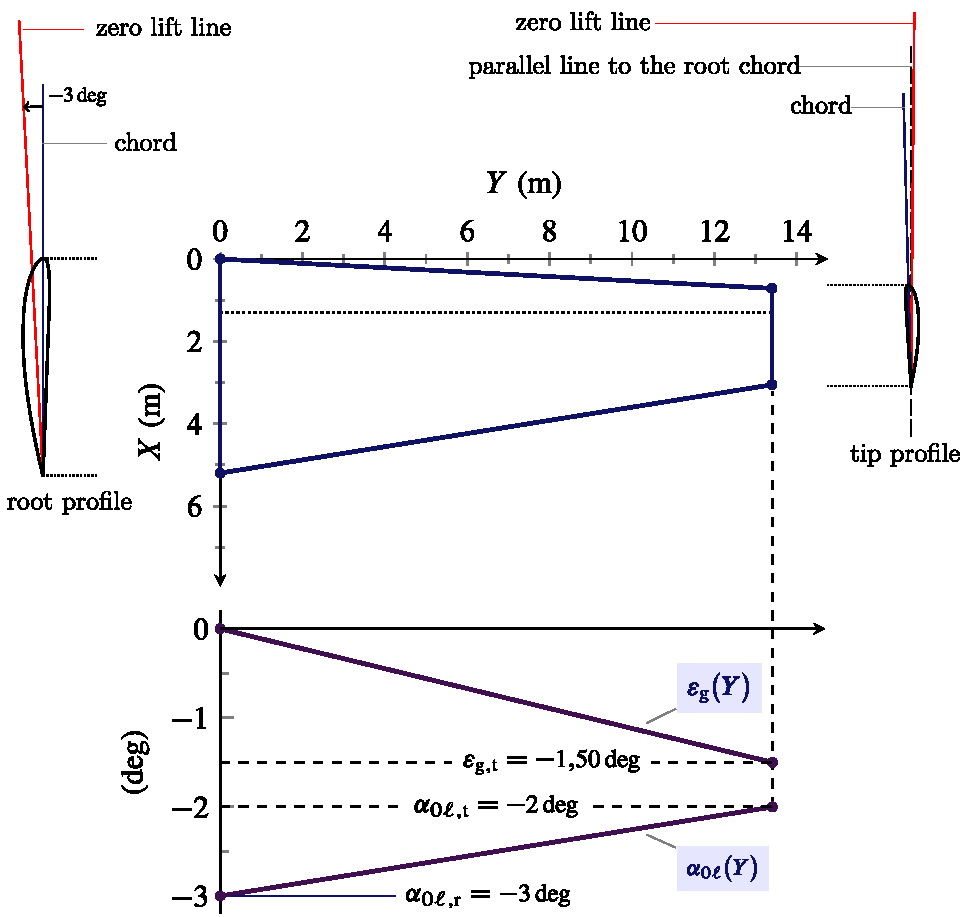
\includegraphics[width=0.78\textwidth]{exercises/wing_alpha_zero_lift_1/wing_alpha_zero_lift_basic_1_drawing.pdf}%
%  \caption{\finalhyphendemerits=1000
%           Forma in pianta della semiala dell'esempio~\ref{example:Wing:Alpha:Zero:Lift:A}.
%           Sono rappresentate le leggi lineari di svergolamento geometrico $\epsilon_\mathrm{g}$ 
%           e di angolo di portanza nulla di sezione $\alpha_{0\ell}$.}
%  \label{fig:Alpha:Zero:Lift:Calculations:A}%
%\end%
%    %{figure}%
%    {SCfigure}%
%
%\EnlargedFigure% needs two latex passes
%    {t}% #1: t, b, p
%    {images/airfoil_geometry}% #2: the image file included by \includegraphics
%    {width=1.0\textwidth}% #3: option list to pass to \includegraphics, e.g. width=\linewidth,rotate=0
%    {\finalhyphendemerits=1000
%      Alcune caratteristiche geometriche di un profilo alare.}% #4: the caption text
%    {fig:Aero:Profilo:Geometria}% #5: the label
\EnlargedFigureX% needs two latex passes
  {t}% #1: t, b, p
  {%
    \makebox[\textwidth][c]{%
    \includegraphics%
      [width=0.95\textwidth]%
      {exercises/wing_alpha_zero_lift_1/wing_alpha_zero_lift_basic_1_drawing.pdf}%
    }% end-of-makebox
  }% #2: the image file included by \includegraphics
  {\finalhyphendemerits=1000
    Forma in pianta della semiala dell'esempio~\ref{example:Wing:Alpha:Zero:Lift:A}.
    Sono rappresentate le leggi lineari di svergolamento geometrico $\epsilon_\mathrm{g}$ 
    e di angolo di portanza nulla di sezione $\alpha_{0\ell}$.
    A sinistra è disegnato lo schema del profilo di radice con la sua retta di portanza nulla e
    la sua corda. Questa è la retta di riferimento per gli angoli $\epsilon_\mathrm{g}(Y)$. 
    A destra è disegnato il profilo d'estremità, calettato di un angolo 
    $\epsilon_{\mathrm{g,t}}=\epsilon_\mathrm{g}(\frac{1}{2}b)$.%
  }% #3: the caption text
  {fig:Alpha:Zero:Lift:Calculations:A}%% #4: the label
%
%-----------------------------------------------------------------------------------------------
%
%--END-EXERCISE:wing_alpha_zero_lift__1
%===============================================================================================

%===============================================================================================
%--BEGIN-EXERCISE:wing_alpha_zero_lift_1_A
%
\def\mySpanWingMT{10.600000}
\def\mySpanWingIMT{6.360000}
\def\mySpanWingIIMT{4.240000}
\def\myChordRootWingMT{1.440000}
\def\myChordRootWingIMT{1.440000}
\def\myChordRootWingIIMT{1.440000}
\def\myChordTipWingMT{0.860000}
\def\myChordTipWingIMT{1.440000}
\def\myChordTipWingIIMT{0.860000}
\def\mySweepLEWingIIDEG{0.000000}
\def\myCoeffAChordWingI{0.000000}
\def\myCoeffBChordWingIMT{1.440000}
\def\myCoeffAChordWingII{-0.273585}
\def\myCoeffBChordWingIIMT{1.440000}
\def\myAlphaZeroLiftRootWingIDEG{-2.500000}
\def\myAlphaZeroLiftTipWingIDEG{-2.500000}
\def\myAlphaZeroLiftRootWingIRAD{-0.043633}
\def\myAlphaZeroLiftTipWingIRAD{-0.043633}
\def\myAlphaZeroLiftRootWingIIDEG{-2.500000}
\def\myAlphaZeroLiftTipWingIIDEG{-1.000000}
\def\myAlphaZeroLiftRootWingIIRAD{-0.043633}
\def\myAlphaZeroLiftTipWingIIRAD{-0.017453}
\def\myTaperRatioWingI{1.000000}
\def\myTaperRatioWingII{0.597222}
\def\myTwistWingIDEG{0.000000}
\def\myTwistWingIRAD{0.000000}
\def\myTwistWingIIDEG{-3.000000}
\def\myTwistWingIIRAD{-0.052360}
\def\myAreaWingIMTsquared{9.158400}
\def\myAreaWingIIMTsquared{4.876000}
\def\myAreaWingMTsquared{14.034400}
\def\myCoeffAAeroTwistWingIRADMT{0.000000}
\def\myCoeffBAeroTwistWingIRAD{-0.043633}
\def\myCoeffAAeroTwistWingIIRADMT{0.012349}
\def\myCoeffBAeroTwistWingIIRAD{-0.043633}
\def\myCoeffATwistWingIRADMT{0.000000}
\def\myCoeffATwistWingIIRADMT{-0.024698}
\def\myCoeffBTwistWingIRAD{0.000000}
\def\myCoeffBTwistWingIIRAD{0.000000}
\def\myAlphaZeroLiftWingIRAD{-0.028653}
\def\myAlphaZeroLiftWingIDEG{-1.641680}
\def\myAlphaZeroLiftWingIIRAD{0.008329}
\def\myAlphaZeroLiftWingIIDEG{0.477233}
\def\myAlphaZeroLiftWingRAD{-0.020323}
\def\myAlphaZeroLiftWingDEG{-1.164447}

%
\begin{myExampleX}{Angolo di portanza nulla di un'ala \emph{cranked}}{\ding{46}}% \ \Keyboard\ %
\label{example:Wing:Alpha:Zero:Lift:AA}
%
\noindent
La semiala destra di un velivolo dell'aviazione generale è rappresentata
nella figura~\ref{fig:Wing:Alpha:Zero:Lift:Results:AA} (si veda anche
l'esercizio~\ref{exercise:Cranked:Wing:Planform:Basic:B}).
La forma in pianta ha il bordo d'attacco rettilineo e il bordo d'uscita
rettilineo a tratti, con discontinuità nel punto $B'$.
L'ala è un caso particolare di \emph{cranked wing} con
$\Lambda_\mathrm{le,1}=\Lambda_\mathrm{le,2}=\SI[round-precision=0]{\mySweepLEWingIIDEG}{\degree}$.

L'apertura totale è $b=\SI[round-precision=1]{\mySpanWingMT}{\metre}$,
il pannello interno ha estensione
$\frac{1}{2}b_1=\calcSI[round-precision=2,fixed-exponent=0,scientific-notation=fixed]{0.5*\mySpanWingIMT}{\metre}$,
il pannello esterno ha estensione
$\frac{1}{2}b_2=\frac{1}{2}b-\frac{1}{2}b_1
=\calcSI[round-precision=2,fixed-exponent=0,scientific-notation=fixed]{0.5*\mySpanWingIIMT}{\metre}$.
La corda del pannello interno è costante e pari a 
$c_\mathrm{r}=c_{\mathrm{r},1}=c_{\mathrm{t},1}=\SI[round-precision=2]{\myChordRootWingMT}{\metre}$.
Il pannello esterno è invece rastremato e ha corda d'estremità
$c_\mathrm{t}=c_{\mathrm{t},2}=\SI[round-precision=2]{\myChordTipWingMT}{\metre}$.

Inoltre, il pannello interno ha profilo e svergolamento geometrico costanti.
Sia alla radice che all'estremità del primo pannello l'angolo di portanza nulla
di sezione è
$\alpha_{0\ell,\mathrm{r},1}=\alpha_{0\ell,\mathrm{t},1}=
\SI[round-precision=1]{\myAlphaZeroLiftRootWingIDEG}{\deg}$
e il calettamento geometrico è
$\epsilon_{\mathrm{g,r},1}=\epsilon_{\mathrm{g,t},1}=\SI[round-precision=0]{\myTwistWingIDEG}{\deg}$.
Nel pannello esterno si ha una variazione lineare dell'angolo di portanza nulla
e dello svergolamento geometrico;
la sezione d'estremità possiede un angolo di portanza nulla
$\alpha_{0\ell,\mathrm{t},2}=\SI[round-precision=1]{\myAlphaZeroLiftTipWingIIDEG}{\deg}$.
e uno svergolamento geometrico 
$\epsilon_{\mathrm{g,t},2}=\SI[round-precision=1]{\myTwistWingIIDEG}{\deg}$.
Si veda la figura~\ref{fig:Wing:Alpha:Zero:Lift:Results:AA} per una rappresentazione grafica
delle leggi $c(Y)$, $\alpha_{0\ell}(Y)$ ed $\epsilon_\mathrm{g}(Y)$.

Si vuole calcolare l'angolo di portanza nulla dell'ala: $\alpha_{0L}$.

\medskip
Per risolvere il problema basta ricostruire le espressioni analitiche delle
delle leggi $c(Y)$, $\alpha_{0\ell}(Y)$ ed $\epsilon_\mathrm{g}(Y)$
per $0\le Y \le \frac{1}{2}b$. Successivamente, tali leggi lineari a tratti 
vanno sostituite nell'integrale definito contenuto nella formula di calcolo
di $\alpha_{0L}$.

La legge delle corde della forma in pianta assegnata è la seguente funzione lineare a tratti:
\[
c(Y)=
\ccases{
%\left\{
%\begin{array}{cl}
c_1(Y) = A_{c,1} \, Y + B_{c,1} & \text{per }\makebox[3em][r]{$0$}     \le Y \le \frac{1}{2}b_1
\\[4pt]
c_2(Y) = A_{c,2} \, \bigg(Y-\dfrac{b_1}{2}\bigg) + B_{c,2} & \text{per }\makebox[3em][r]{$\frac{1}{2}b_1$}< Y \le \frac{1}{2}b
%\end{array}
%\right.
}
\]
i cui coefficienti si calcolano imponendo $c_1(0)=c_{\mathrm{r},1}$,
$c_1(\frac{1}{2}b_1)=c_{\mathrm{t},1}$, $c_2(\frac{1}{2}b_1)=c_{\mathrm{r},2}$, $c_2(\frac{1}{2}b)=c_{\mathrm{t},2}$.
Per i dati assegnati si ha
\[
A_{c,1}
  = \frac{c_{\mathrm{t},1} - c_{\mathrm{r},1}}{b_1/2}
  = 
    2 \frac{
      \SI[round-precision=2]{\myChordTipWingIMT}{\metre} - \SI[round-precision=2]{\myChordRootWingIMT}{\metre}
    }{
      \SI[round-precision=2]{\mySpanWingIMT}{\metre}
    }
  = \mathunderline{mydarkblue}{ \SI[round-precision=3]{\myCoeffAChordWingI}{} }
\]
\[
B_{c,1}
  = c_{\mathrm{r},1}
  = \mathunderline{mydarkblue}{ \SI[round-precision=2]{\myCoeffBChordWingIMT}{\metre} }
\]
\[
A_{c,2}
  = \frac{c_{\mathrm{t},2} - c_{\mathrm{r},2}}{b_2/2}
  = 
    2 \frac{
      \SI[round-precision=2]{\myChordTipWingIIMT}{\metre} - \SI[round-precision=2]{\myChordRootWingIIMT}{\metre}
    }{
      \SI[round-precision=2]{\mySpanWingIIMT}{\metre}
    }
  = \mathunderline{mydarkblue}{ \SI[round-precision=3]{\myCoeffAChordWingII}{} }
\]
\[
B_{c,2}
  = c_{\mathrm{r},2}
  = \mathunderline{mydarkblue}{ \SI[round-precision=2]{\myCoeffBChordWingIIMT}{\metre} }
\]
dunque
\[
c(Y)=
\ccases{
%\left\{
%\begin{array}{cl}
c_1(Y) = 
  %% ZERO -> \SI[round-precision=3]{\myCoeffAChordWingI}{} \, Y 
    % + 
    \SI[round-precision=2]{\myCoeffBChordWingIIMT}{\metre} 
  & \text{per }
    \makebox[3.5em][r]{$\SI[round-precision=0]{0}{\metre}$} 
      \le Y \le 
      \calcSI[round-precision=2,fixed-exponent=0,scientific-notation=fixed]{0.5*\mySpanWingIMT}{\metre}
\\[4pt]
c_2(Y) 
  = \SI[round-precision=3]{\myCoeffAChordWingII}{} \, 
    \big(
      Y
      - \calcSI[round-precision=2,fixed-exponent=0,scientific-notation=fixed]{0.5*\mySpanWingIMT}{\metre}
    \big)
    + \SI[round-precision=2]{\myCoeffBChordWingIIMT}{\metre} 
  & \text{per }
    \makebox[3.5em][r]{%
      $\calcSI[round-precision=2,fixed-exponent=0,scientific-notation=fixed]{0.5*\mySpanWingIMT}{\metre}$
    }% end-of-makebox
      < Y 
      \le \calcSI[round-precision=2,fixed-exponent=0,scientific-notation=fixed]{0.5*\mySpanWingMT}{\metre}
%\end{array}
%\right.
}
\]

La legge degli angoli di portanza nulla di sezione è la seguente funzione lineare a tratti:
\[
\alpha_{0\ell}(Y)=
\ccases{
%\left\{
%\begin{array}{cl}
\alpha_{0\ell,1}(Y) = A_{\alpha,1} \, Y + B_{\alpha,1} & \text{per }\makebox[3em][r]{$0$}     \le Y \le \frac{1}{2}b_1
\\[4pt]
\alpha_{0\ell,2}(Y) = A_{\alpha,2} \, \bigg(Y-\dfrac{b_1}{2}\bigg) + B_{\alpha,2} & \text{per }\makebox[3em][r]{$\frac{1}{2}b_1$}< Y \le \frac{1}{2}b
%\end{array}
%\right.
}
\]
i cui coefficienti si calcolano imponendo $\alpha_{0\ell,1}(0)=\alpha_{0\ell,\mathrm{r},1}$,
$\alpha_{0\ell,1}(\frac{1}{2}b_1)=\alpha_{0\ell,\mathrm{t},1}$, $\alpha_{0\ell,2}(\frac{1}{2}b_1)=\alpha_{0\ell,\mathrm{r},2}$, $\alpha_{0\ell,2}(\frac{1}{2}b)=\alpha_{0\ell,\mathrm{t},2}$.
Per i dati assegnati si ha
\[
A_{\alpha,1}
  = \frac{\alpha_{0\ell,\mathrm{t},1} - \alpha_{0\ell,\mathrm{r},1}}{b_1/2}
  = 
    2 \frac{
      \SI[round-precision=2]{\myAlphaZeroLiftTipWingIRAD}{\radian} - ( \SI[round-precision=2]{\myAlphaZeroLiftRootWingIRAD}{\radian} )
    }{
      \SI[round-precision=2]{\mySpanWingIMT}{\metre}
    }
  = \mathunderline{mydarkblue}{ \SI[round-precision=3]{\myCoeffAAeroTwistWingIRADMT}{\radian/\metre} }
\]
\[
B_{\alpha,1}
  = \alpha_{0\ell,\mathrm{r},1}
  = \mathunderline{mydarkblue}{ \SI[round-precision=4]{\myCoeffBAeroTwistWingIRAD}{\radian} }
\]
\[
A_{\alpha,2}
  = \frac{\alpha_{0\ell,\mathrm{t},2} - \alpha_{0\ell,\mathrm{r},2}}{b_2/2}
  = 
    2 \frac{
      \SI[round-precision=4]{\myAlphaZeroLiftTipWingIIRAD}{\metre} - ( \SI[round-precision=4]{\myAlphaZeroLiftRootWingIIRAD}{\metre} )
    }{
      \SI[round-precision=2]{\mySpanWingIIMT}{\metre}
    }
  = \mathunderline{mydarkblue}{ \SI[round-precision=4]{\myCoeffAAeroTwistWingIIRADMT}{\radian/\metre} }
\]
\[
B_{\alpha,2}
  = \alpha_{0\ell,\mathrm{r},2}
  = \mathunderline{mydarkblue}{ \SI[round-precision=4]{\myCoeffBAeroTwistWingIIRAD}{\radian} }
\]
dunque
\[
\alpha_{0\ell}(Y)=
\ccases{
%\left\{
%\begin{array}{cl}
\alpha_{0\ell,1}(Y) = 
  %% ZERO -> \SI[round-precision=3]{\myCoeffAAeroTwistWingIRADMT}{\radian/\metre} \, Y 
    % + 
    \SI[round-precision=4]{\myCoeffBAeroTwistWingIRAD}{\radian} 
  & \text{per }
    \makebox[3.5em][r]{$\SI[round-precision=0]{0}{\metre}$} 
      \le Y \le 
      \calcSI[round-precision=2,fixed-exponent=0,scientific-notation=fixed]{0.5*\mySpanWingIMT}{\metre}
\\[4pt]
\alpha_{0\ell,2}(Y) 
  = \SI[round-precision=4]{\myCoeffAAeroTwistWingIIRADMT}{\radian/\metre} \; 
    \big(
      Y
      - \calcSI[round-precision=2,fixed-exponent=0,scientific-notation=fixed]{0.5*\mySpanWingIMT}{\metre}
    \big)
   %% + \SI[round-precision=4]{\myCoeffBAeroTwistWingIIRAD}{\radian} 
   \rule{2em}{0pt}% --> SPACER
%
\\
    \hfill
    \SI[round-precision=4]{\myCoeffBAeroTwistWingIIRAD}{\radian}
%
  & \text{per }
    \makebox[3.5em][r]{%
      $\calcSI[round-precision=2,fixed-exponent=0,scientific-notation=fixed]{0.5*\mySpanWingIMT}{\metre}$
    }% end-of-makebox
      < Y 
      \le \calcSI[round-precision=2,fixed-exponent=0,scientific-notation=fixed]{0.5*\mySpanWingMT}{\metre}
%\end{array}
%\right.
}
\]

Infine, la legge degli angoli di svergolamento geometrico di sezione è la seguente funzione lineare a tratti:
\[
\epsilon_{\mathrm{g}}(Y)=
\ccases{
%\left\{
%\begin{array}{cl}
\epsilon_{\mathrm{g},1}(Y) = A_{\epsilon,1} \, Y + B_{\epsilon,1} & \text{per }\makebox[3em][r]{$0$}     \le Y \le \frac{1}{2}b_1
\\[4pt]
\epsilon_{\mathrm{g},2}(Y) = A_{\epsilon,2} \, \bigg(Y-\dfrac{b_1}{2}\bigg) + B_{\epsilon,2} & \text{per }\makebox[3em][r]{$\frac{1}{2}b_1$}< Y \le \frac{1}{2}b
%\end{array}
%\right.
}
\]
i cui coefficienti si calcolano imponendo $\epsilon_{\mathrm{g},1}(0)=\SI[round-precision=0]{0}{\deg}$,
$\epsilon_{\mathrm{g},1}(\frac{1}{2}b_1)=\epsilon_{\mathrm{g,t},1}$, $\epsilon_{\mathrm{g},2}(\frac{1}{2}b_1)=\epsilon_{\mathrm{g,t},1}$, $\epsilon_{\mathrm{g},2}(\frac{1}{2}b)=\epsilon_{\mathrm{g,t},2}$.
Per i dati assegnati si ha
\[
A_{\epsilon,1}
  = \frac{\epsilon_{\mathrm{g,t},1}}{b_1/2}
  = 
    2 \frac{
      \SI[round-precision=2]{\myTwistWingIRAD}{\radian}
    }{
      \SI[round-precision=2]{\mySpanWingIMT}{\metre}
    }
  = \mathunderline{mydarkblue}{ \SI[round-precision=3]{\myCoeffATwistWingIRADMT}{\radian/\metre} }
\]
\[
B_{\epsilon,1}
  = \epsilon_{\mathrm{g,r},1}
  = \mathunderline{mydarkblue}{ \SI[round-precision=4]{\myCoeffBTwistWingIRAD}{\radian} }
\]
\[
A_{\epsilon,2}
  = \frac{\epsilon_{\mathrm{g,t},2} - \epsilon_{\mathrm{g,r},2}}{b_2/2}
  = 
    2 \frac{
      \SI[round-precision=4]{\myTwistWingIIRAD}{\metre} - ( \SI[round-precision=4]{\myTwistWingIRAD}{\metre} )
    }{
      \SI[round-precision=2]{\mySpanWingIIMT}{\metre}
    }
  = \mathunderline{mydarkblue}{ \SI[round-precision=4]{\myCoeffATwistWingIIRADMT}{\radian/\metre} }
\]
\[
B_{\epsilon,2}
  = \epsilon_{\mathrm{g,r},2}
  = \mathunderline{mydarkblue}{ \SI[round-precision=2]{\myCoeffBTwistWingIIRAD}{\radian} }
\]
dunque
\[
\epsilon_{\mathrm{g}}(Y)=
\ccases{
%\left\{
%\begin{array}{cl}
\epsilon_{\mathrm{g},1}(Y) = 
  %% ZERO -> \SI[round-precision=3]{\myCoeffAAeroTwistWingIRADMT}{\radian/\metre} \, Y 
    % + 
    \SI[round-precision=4]{\myCoeffBTwistWingIRAD}{\radian} 
  & \text{per }
    \makebox[3.5em][r]{$\SI[round-precision=0]{0}{\metre}$} 
      \le Y \le 
      \calcSI[round-precision=2,fixed-exponent=0,scientific-notation=fixed]{0.5*\mySpanWingIMT}{\metre}
\\[4pt]
\epsilon_{\mathrm{g},2}(Y) 
  = \SI[round-precision=4]{\myCoeffATwistWingIIRADMT}{\radian/\metre} \; 
    \big(
      Y
      - \calcSI[round-precision=2,fixed-exponent=0,scientific-notation=fixed]{0.5*\mySpanWingIMT}{\metre}
    \big)
   %% + \SI[round-precision=4]{\myCoeffBAeroTwistWingIIRAD}{\radian} 
%   \rule{2em}{0pt}% --> SPACER
%
% \\
%    \hfill
%    \SI[round-precision=4]{\myCoeffBTwistWingIIRAD}{\radian}
%
  & \text{per }
    \makebox[3.5em][r]{%
      $\calcSI[round-precision=2,fixed-exponent=0,scientific-notation=fixed]{0.5*\mySpanWingIMT}{\metre}$
    }% end-of-makebox
      < Y 
      \le \calcSI[round-precision=2,fixed-exponent=0,scientific-notation=fixed]{0.5*\mySpanWingMT}{\metre}
%\end{array}
%\right.
}
\]

A questo punto è possibile calcolare l'angolo di portanza nulla
\[
\alpha_{0L} 
  = \frac{2}{S} \int_0^{b/2} 
    \Big[ 
      \alpha_{0\ell}\big(Y\big) - \epsilon_\mathrm{g}\big(Y\big) 
    \Big] \, c(Y) \diff{Y}
\]
che per un'ala \emph{cranked} a due pannelli diventa una somma di due integrali
\[
\begin{split}
\alpha_{0L} 
  & {}= 
    \frac{2}{S} \int_0^{b_1/2} 
    \Big[ 
      \alpha_{0\ell,1}\big(Y\big) - \epsilon_{\mathrm{g},1}\big(Y\big) 
    \Big] \, c_1(Y) \diff{Y}
\\[3pt]
  &
  \rule{0.25\linewidth}{0pt}% --> SPACER
  +
    \frac{2}{S} \int_{b_1/2}^{b/2}
    \Big[ 
      \alpha_{0\ell,2}\big(Y\big) - \epsilon_{\mathrm{g},2}\big(Y\big) 
    \Big] \, c_2(Y) \diff{Y}
\end{split}
\]
La formula precedente, scritta per esteso, diventa
\[
\begin{split}
\alpha_{0L} 
  & {}= \frac{2}{S} \int_0^{b_1/2} 
    \bigg[ \Big( A_{\alpha,1} \, Y + B_{\alpha,1} \Big) - A_{\epsilon,1} \, Y \bigg] \Big( A_{c,1} Y + B_{c,1} \Big)
      \diff{Y} \hfill \mbox{}
\\[3pt]
  &  
    \rule{3em}{0pt}% --> SPACER
    %\mbox{} \hfill 
    + \frac{2}{S} \int_{b_1/2}^{b/2} 
    \bigg[ A_{\alpha,2} \, \Big( Y - \frac{b_1}{2} \Big) + B_{\alpha,2} 
      - A_{\epsilon,2} \, \Big( Y - \frac{b_1}{2} \Big) - B_{\epsilon,2}\bigg] 
   \rule{1em}{0pt}% --> SPACER
\\[3pt]
  &  
    \rule{22em}{0pt}% --> SPACER
    \cdot \bigg[ A_{c,2} \Big( Y - \frac{b_1}{2} \Big) + B_{c,2} \bigg]
      \diff{Y}
\end{split}
\]

I pannelli della semiala assegnata hanno un rapporti di rastremazione
\[
\lambda_1
  =\frac{c_{\mathrm{t},1}}{c_{\mathrm{r},1}}
  =\frac{\SI[round-precision=2]{\myChordTipWingIMT}{\metre}}{\SI[round-precision=2]{\myChordRootWingIMT}{\metre}}
  =\mathunderline{mydarkblue}{ \SI[round-precision=2]{\myTaperRatioWingI}{} }
\]
\[
\lambda_2
  =\frac{c_{\mathrm{t},2}}{c_{\mathrm{r},2}}
  =\frac{\SI[round-precision=2]{\myChordTipWingIIMT}{\metre}}{\SI[round-precision=2]{\myChordRootWingIIMT}{\metre}}
  =\mathunderline{mydarkblue}{ \SI[round-precision=2]{\myTaperRatioWingII}{} }
\]
e superfici
\[
\begin{split}
S_1 & {}= \frac{b_1}{2} \, c_{\mathrm{r},1} \, \big( 1 + \lambda_1 \big) \\
  & {}=
    \num{0.5} \cdot \SI[round-precision=1]{\mySpanWingIMT}{\metre}
      \cdot \SI[round-precision=2]{\myChordRootWingIMT}{\metre}
      \cdot \big( 1 + \SI[round-precision=2]{\myTaperRatioWingI}{} \big) 
    = \mathunderline{mydarkblue}{ \SI[round-precision=1]{\myAreaWingIMTsquared}{\metre^2} }
\end{split}
\]
\[
\begin{split}
S_2 & {}= \frac{b_2}{2} \, c_{\mathrm{r},2} \, \big( 1 + \lambda_2 \big) \\
  & {}=
    \num{0.5} \cdot \SI[round-precision=1]{\mySpanWingIIMT}{\metre}
      \cdot \SI[round-precision=2]{\myChordRootWingIIMT}{\metre}
      \cdot \big( 1 + \SI[round-precision=2]{\myTaperRatioWingII}{} \big) 
    = \mathunderline{mydarkblue}{ \SI[round-precision=1]{\myAreaWingIIMTsquared}{\metre^2} }
\end{split}
\]
Pertanto, la superficie alare è
\[
\begin{split}
S = S_1 + S_2 
  = \SI[round-precision=1]{\myAreaWingIMTsquared}{\metre^2}
    + \SI[round-precision=1]{\myAreaWingIIMTsquared}{\metre^2}
  = \mathunderline{mydarkblue}{ \SI[round-precision=1]{\myAreaWingMTsquared}{\metre^2} }
\end{split}
\]

La somma dei due integrali definiti è facilmente ottenibile sostituendo nelle funzioni integrande i valori
dei coefficienti precedentemente calcolati.
Svolgendo i calcoli per il primo integrale si ottiene
\[
\begin{split}
\alpha_{0L,1} 
  & {}= \frac{2}{S} \int_0^{b_1/2} 
    \bigg[ \Big( A_{\alpha,1} \, Y + B_{\alpha,1} \Big) - A_{\epsilon,1} \, Y \bigg] \Big( A_{c,1} Y + B_{c,1} \Big)
      \diff{Y} \hfill \mbox{}
\\[3pt]
   & ={}
     \frac{2}{ \SI[round-precision=1]{\myAreaWingMTsquared}{\metre^2} }
     \int_{\SI{0}{m}}^{
       \calcSI[round-precision=1,fixed-exponent=0,scientific-notation=fixed]{0.5*\mySpanWingIMT}{\metre}
     }
     \Big[ 
       \Big( 
         % A_{\alpha} \, Y + B_{\alpha} 
         \SI[round-precision=5]{\myCoeffAAeroTwistWingIRADMT}{\radian/\metre} \; Y
           \SI[round-precision=4]{\myAlphaZeroLiftRootWingIRAD}{\radian}
       \Big) 
\\
  & \rule{0.3\linewidth}{0pt}% --> SPACER
       % - A_{\epsilon} \, Y 
       - ( \SI[round-precision=5]{\myCoeffATwistWingIRADMT}{\radian/\metre} ) \; Y
     \Big] 
     \Big( 
       \SI[round-precision=3]{\myCoeffAChordWingI}{} \; Y
         + \SI[round-precision=2]{\myCoeffBChordWingIMT}{\metre}
       \Big) \diff{Y}
\\
   & ={}
     \frac{2}{ \SI[round-precision=1]{\myAreaWingMTsquared}{\metre^2} }
     \int_{\SI{0}{m}}^{
       \calcSI[round-precision=1,fixed-exponent=0,scientific-notation=fixed]{0.5*\mySpanWingIMT}{\metre}
     }
           \SI[round-precision=4]{\myAlphaZeroLiftRootWingIRAD}{\radian}
         \cdot \SI[round-precision=2]{\myCoeffBChordWingIMT}{\metre}
       \diff{Y}
\\[2pt]
  & {}= \mathunderline{mydarkblue}{ \SI[round-precision=4]{\myAlphaZeroLiftWingIRAD}{\radian} }
  = \mathunderline{mydarkblue}{ \SI[round-precision=2]{\myAlphaZeroLiftWingIDEG}{\deg} }
\end{split}
\]

Analogamente, per il secondo integrale si ottiene
\[
\begin{split}
\alpha_{0L,2} 
  & {}= \frac{2}{S} \int_{b_1/2}^{b/2} 
    \bigg[ A_{\alpha,2} \, \Big( Y - \frac{b_1}{2} \Big) + B_{\alpha,2} 
      - A_{\epsilon,2} \, \Big( Y - \frac{b_1}{2} \Big) - B_{\epsilon,2}\bigg] 
   \rule{1em}{0pt}% --> SPACER
\\[3pt]
  &  
    \rule{22em}{0pt}% --> SPACER
    \cdot \bigg[ A_{c,2} \Big( Y - \frac{b_1}{2} \Big) + B_{c,2} \bigg]
      \diff{Y}
\\
  & ={}
    \frac{2}{ \SI[round-precision=1]{\myAreaWingMTsquared}{\metre^2} }
    \int_{
      \calcSI[round-precision=1,fixed-exponent=0,scientific-notation=fixed]{0.5*\mySpanWingIMT}{\metre}
    }^{
      \calcSI[round-precision=1,fixed-exponent=0,scientific-notation=fixed]{0.5*\mySpanWingMT}{\metre}
    }
    \Big[ 
      % A_{\alpha} \, Y + B_{\alpha} 
      \SI[round-precision=4]{\myCoeffAAeroTwistWingIIRADMT}{\radian/\metre} \; \Big( Y
        - \calcSI[round-precision=1,fixed-exponent=0,scientific-notation=fixed]{0.5*\mySpanWingIMT}{\metre} \Big)
        \SI[round-precision=4]{\myAlphaZeroLiftRootWingIIRAD}{\radian}
\\
  & \rule{0.3\linewidth}{0pt}% --> SPACER
       % - A_{\epsilon} \, Y 
       - ( \SI[round-precision=4]{\myCoeffATwistWingIIRADMT}{\radian/\metre} ) \; \Big( Y
           - \calcSI[round-precision=1,fixed-exponent=0,scientific-notation=fixed]{0.5*\mySpanWingIMT}{\metre} \Big)
           - \SI[round-precision=2]{\myCoeffBTwistWingIIRAD}{\radian}
     \Big]
\\
  & \rule{0.5\linewidth}{0pt}% --> SPACER
     \Big[ 
       \SI[round-precision=3]{\myCoeffAChordWingII}{} \; \Big( Y
           - \calcSI[round-precision=1,fixed-exponent=0,scientific-notation=fixed]{0.5*\mySpanWingIMT}{\metre} \Big)
         + \SI[round-precision=2]{\myCoeffBChordWingIIMT}{\metre}
       \Big] \diff{Y}
\\[2pt]
  & {}= \mathunderline{mydarkblue}{ \SI[round-precision=5]{\myAlphaZeroLiftWingIIRAD}{\radian} }
  = \mathunderline{mydarkblue}{ \SI[round-precision=2]{\myAlphaZeroLiftWingIIDEG}{\deg} }
\end{split}
\]

Infine, l'angolo di portanza nulla dell'ala assegnata è
\[
\begin{split}
\alpha_{0L} = \alpha_{0L,1} + \alpha_{0L,2} 
  & {}= \SI[round-precision=4]{\myAlphaZeroLiftWingIRAD}{\radian}
    + ( \SI[round-precision=5]{\myAlphaZeroLiftWingIIRAD}{\radian} )
\\
  & {}= \mathunderline{mydarkblue}{ \SI[round-precision=4]{\myAlphaZeroLiftWingRAD}{\radian} }
    = \mathunderline{mydarkblue}{ \SI[round-precision=2]{\myAlphaZeroLiftWingDEG}{\deg} }
\end{split}
\]

\end{myExampleX}

%-----------------------------------------------------------------------------------------------
\begin%
  %{figure}
  {SCfigure}[1.9]%
  [t]%[H]%[!htbp]
  %\centering
  %\checkoddpage
  %\centering
    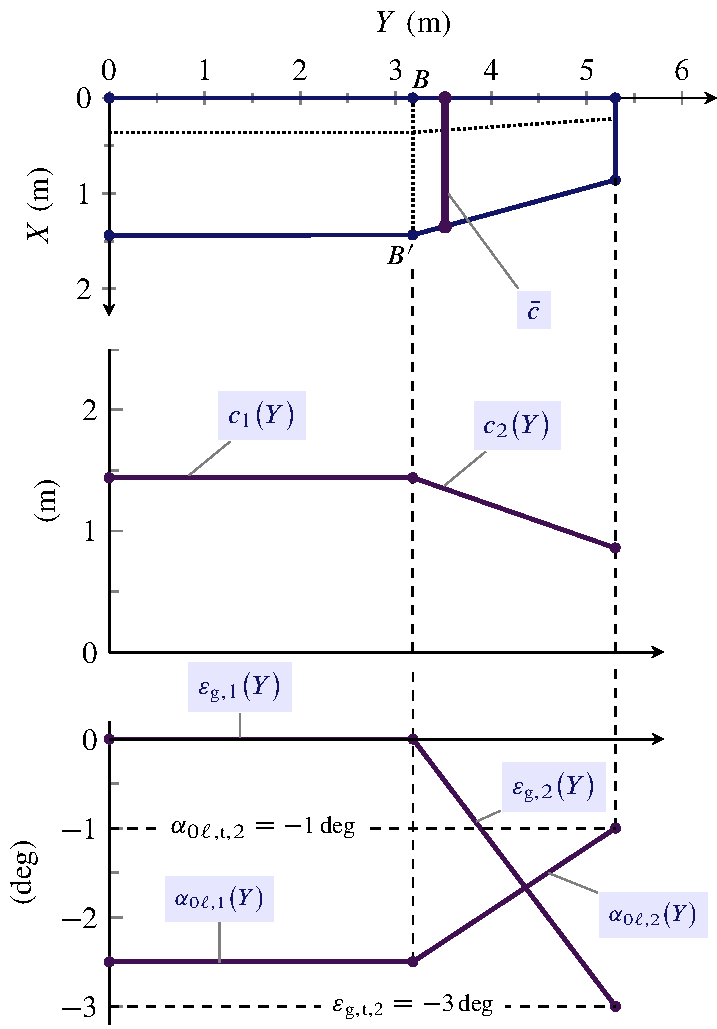
\includegraphics[width=0.78\textwidth]{exercises/wing_alpha_zero_lift_1A/wing_alpha_zero_lift_1A_drawing.pdf}%
  \caption{\finalhyphendemerits=1000
           Forma in pianta dell'ala \emph{cranked} assegnata nell'esempio~\ref{example:Wing:Alpha:Zero:Lift:AA}.
           Sono riportate anche le leggi lineari a tratti della corda, dell'angolo di portanza nulla di sezione
           e dello svergolamento geometrico.%
  }
  \label{fig:Wing:Alpha:Zero:Lift:Results:AA}%
\end%
    %{figure}%
    {SCfigure}%
%
%\EnlargedFigure% needs two latex passes
%    {t}% #1: t, b, p
%    {images/airfoil_geometry}% #2: the image file included by \includegraphics
%    {width=1.0\textwidth}% #3: option list to pass to \includegraphics, e.g. width=\linewidth,rotate=0
%    {\finalhyphendemerits=1000
%      Alcune caratteristiche geometriche di un profilo alare.}% #4: the caption text
%    {fig:Aero:Profilo:Geometria}% #5: the label
%\EnlargedFigureX% needs two latex passes
%  {t}% #1: t, b, p
%  {%
%    \makebox[\textwidth][c]{%
%    \includegraphics%
%      %[width=0.52\textwidth]%
%      % [height=5.5cm]%
%      [width=0.485\textwidth]%
%      {images/airfoil_Re_effect_polar.pdf}%
%    %\rule{8mm}{0pt}% <-- SPACER
%    \hfill
%    \raisebox{-0.6mm}[0pt][0pt]{%
%    \includegraphics%
%      %[width=0.52\textwidth]%
%      % [height=5.5cm]%
%      [width=0.485\textwidth]%
%      {images/airfoil_Re_effect_alpha_Cl.pdf}
%    }% end-of-raisebox
%    }% end-of-makebox
%  }% #2: the image file included by \includegraphics
%  {\finalhyphendemerits=1000
%    Influenza del numero di Reynolds, $\Reynolds_{\infty}=V_{\!\infty}c/\nu_{\infty}$,
%           sulla polare e sulla curva di portanza di un profilo NACA 64-212.%
%  }% #3: the caption text
%  {fig:Airfoil:Reynolds:Effects}%% #4: the label
%
%-----------------------------------------------------------------------------------------------
%
%--END-EXERCISE:wing_alpha_zero_lift_1_A
%===============================================================================================

\begin{comment}

%===============================================================================================
%--BEGIN-EXERCISE:wing_alpha_zero_lift_2
%
\def\mySpanWingMT{10.600000}
\def\mySpanWingIMT{6.360000}
\def\mySpanWingIIMT{4.240000}
\def\myChordRootWingMT{1.440000}
\def\myChordRootWingIMT{1.440000}
\def\myChordRootWingIIMT{1.440000}
\def\myChordTipWingMT{0.860000}
\def\myChordTipWingIMT{1.440000}
\def\myChordTipWingIIMT{0.860000}
\def\mySweepLEWingIIDEG{0.000000}
\def\myCoeffAChordWingI{0.000000}
\def\myCoeffBChordWingIMT{1.440000}
\def\myCoeffAChordWingII{-0.273585}
\def\myCoeffBChordWingIIMT{1.440000}
\def\myAlphaZeroLiftRootWingIDEG{-2.500000}
\def\myAlphaZeroLiftTipWingIDEG{-2.500000}
\def\myAlphaZeroLiftRootWingIRAD{-0.043633}
\def\myAlphaZeroLiftTipWingIRAD{-0.043633}
\def\myAlphaZeroLiftRootWingIIDEG{-2.500000}
\def\myAlphaZeroLiftTipWingIIDEG{-1.000000}
\def\myAlphaZeroLiftRootWingIIRAD{-0.043633}
\def\myAlphaZeroLiftTipWingIIRAD{-0.017453}
\def\myTaperRatioWingI{1.000000}
\def\myTaperRatioWingII{0.597222}
\def\myTwistWingIDEG{0.000000}
\def\myTwistWingIRAD{0.000000}
\def\myTwistWingIIDEG{-3.000000}
\def\myTwistWingIIRAD{-0.052360}
\def\myAreaWingIMTsquared{9.158400}
\def\myAreaWingIIMTsquared{4.876000}
\def\myAreaWingMTsquared{14.034400}
\def\myCoeffAAeroTwistWingIRADMT{0.000000}
\def\myCoeffBAeroTwistWingIRAD{-0.043633}
\def\myCoeffAAeroTwistWingIIRADMT{0.012349}
\def\myCoeffBAeroTwistWingIIRAD{-0.043633}
\def\myCoeffATwistWingIRADMT{0.000000}
\def\myCoeffATwistWingIIRADMT{-0.024698}
\def\myCoeffBTwistWingIRAD{0.000000}
\def\myCoeffBTwistWingIIRAD{0.000000}
\def\myAlphaZeroLiftWingIRAD{-0.028653}
\def\myAlphaZeroLiftWingIDEG{-1.641680}
\def\myAlphaZeroLiftWingIIRAD{0.008329}
\def\myAlphaZeroLiftWingIIDEG{0.477233}
\def\myAlphaZeroLiftWingRAD{-0.020323}
\def\myAlphaZeroLiftWingDEG{-1.164447}

%
\begin{myExampleX}{Angolo di portanza nulla di un'ala finita (metodo grafico)}{\ding{46}\ \myIconGraph\ }% \ \Keyboard\ %
\label{example:Wing:Alpha:Zero:Lift:B}

\noindent
Si consideri ancora l'ala dell'esempio~\ref{example:Wing:Basic:A}
avente bordi d'attacco e d'uscita rettilinei,
apertura $b=\SI[round-precision=1]{\mySpanWingMT}{\metre}$,
corda di radice $c_\mathrm{r}=\SI[round-precision=2]{\myChordRootWingMT}{\metre}$,
corda d'estremità $c_\mathrm{t}=\SI[round-precision=2]{\myChordTipWingMT}{\metre}$
e freccia del bordo d'attacco
$\Lambda_\mathrm{le}=\SI[round-precision=1]{\mySweepLEWingDEG}{\deg}$.
Inoltre, il profilo di radice ha un angolo di portanza nulla
$\alpha_{0\ell,\mathrm{r}}=\SI[round-precision=1]{\myAlphaZeroLiftRootWingDEG}{\deg}$
mentre il profilo d'estremità ha un angolo di portanza nulla
$\alpha_{0\ell,\mathrm{t}}=\SI[round-precision=1]{\myAlphaZeroLiftTipWingDEG}{\deg}$,
con svergolamento geometrico
$\epsilon_{\mathrm{g,t}}=\SI[round-precision=1]{\myTwistWingDEG}{\deg}$.
Infine, il numero di Mach di volo è $\Mach=\SI[round-precision=2]{\myMach}{}$.

Si vuole calcolare l'angolo di portanza nulla dell'ala $\alpha_{0L}$ 
secondo la formula semiempirica
\begin{equation}
\label{eq:Wing:Alpha:Zero:Lift:Roskam:Datcom}
\alpha_{0L} =
  \Big(
    \bar{\alpha}_{0\ell} + K_{\alpha,1} \, \epsilon_{\mathrm{g,t}}
  \Big) 
  \, K_{\alpha,2}
\end{equation}
In questa modellazione
\[
\bar{\alpha}_{0\ell} = \frac{2}{S} \int_0^{b/2} \alpha_{0\ell}(Y)\, c(Y) \diff{Y}
\]
è il valor medio dell'angolo di portanza nulla di sezione.
Il coefficiente
$K_{\alpha,1}$ è concettualmente il rapporto
$\upDelta\alpha_{0L}/\epsilon_{\mathrm{g,t}}$ che si legge dalla
figura~\ref{fig:Wing:DalphaZeroLift:Roskam:Plots},
funzione dell'angolo di freccia $\Lambda_{c/4}$, dell'allungamento alare $\AR$
e del rapporto di rastremazione $\lambda$.
Il coefficiente
$K_{\alpha,2}$ è un fattore di correzione dovuto agli eventuali
effetti della comprimibilità, si legge dalla figura~\ref{fig:Alpha:Zero:Lift:PrandtlGlauert:Scale:Plots}
ed è funzione del numero di Mach di volo, ovvero del prodotto $\Mach\cos\Lambda_{c/4}$,
e del valor medio dello spessore percentuale dei profili $\overline{(t/c)}$.
%\[
%\overline{(t/c)}
%  = \frac{2}{S} \int_0^{b/2} \left(\frac{t}{c}\right)(Y)\, c(Y) \diff{Y}
%\]

\medskip

Vanno ricostruite le leggi di variazione lungo l'apertura:%
\begin{inparaenum}[(\itshape i\normalfont)]
\item
della corda,
\item
dell'angolo di portanza nulla di sezione, 
\item
dello spessore percentuale di sezione.
\end{inparaenum}
In mancanza di specifiche indicazioni, si può assumere
che le ultime due leggi siano lineari.

Nell'esempio~\ref{example:Wing:Basic:A}, per quanto riguarda le corde, si è ricavato che
\[
A_c
  = \mathunderline{mydarkblue}{ \SI[round-precision=3]{\myCoeffAChordWing}{} }
\;,\quad
B_c
  = \mathunderline{mydarkblue}{ \SI[round-precision=2]{\myCoeffBChordWingMT}{\metre} }
\]
e
\[
c \big( Y \big) = A_c \, Y + B_c
  = \SI[round-precision=3]{\myCoeffAChordWing}{} \, Y
    + \SI[round-precision=2]{\myCoeffBChordWingMT}{\metre}
\]

Per gli angoli di portanza nulla di sezione vale la legge lineare
$\alpha_{0\ell} \big( Y \big) = A_{\alpha} \, Y + B_{\alpha}$ 
con
\[
A_{\alpha}
  = \frac{\alpha_{0\ell,\mathrm{t}} - \alpha_{0\ell\mathrm{r}}}{b/2}
  = 
    2 \frac{
      \SI[round-precision=4]{\myAlphaZeroLiftTipWingRAD}{\radian} 
        - ( \SI[round-precision=4]{\myAlphaZeroLiftRootWingRAD}{\radian} )
    }{
      \SI[round-precision=2]{\mySpanWingMT}{\metre}
    }
  = \mathunderline{mydarkblue}{ \SI[round-precision=5]{\myCoeffAAeroTwistWingRADMT}{\radian/\metre} }
\]
\[
B_{\alpha}
  = \alpha_{0\ell,\mathrm{r}}
  = \mathunderline{mydarkblue}{ \SI[round-precision=4]{\myAlphaZeroLiftRootWingRAD}{\radian} }
\]
dunque
\[
\alpha_{0\ell} \big( Y \big) = A_{\alpha} \, Y + B_{\alpha}
  = (\SI[round-precision=5]{\myCoeffAAeroTwistWingRADMT}{\radian/\metre}) \, Y
    \SI[round-precision=4]{\myAlphaZeroLiftRootWingRAD}{\radian}
\]

La legge dello spessore percentuale dei profili si ricava analogamente,
ponendo
$(t/c)\,\big( Y \big) = A_{t/c} \, Y + B_{t/c}$ 
con
\[
A_{t/c}
  = \frac{(t/c)_{\mathrm{t}} - (t/c)_{\mathrm{r}}}{b/2}
  = 
    2 \frac{
      \SI[round-precision=2]{\myThicknessOverChordTipWing}{} 
        - \SI[round-precision=4]{\myThicknessOverChordRootWing}{}
    }{
      \SI[round-precision=2]{\mySpanWingMT}{\metre}
    }
  = \mathunderline{mydarkblue}{ \SI[round-precision=5]{\myCoeffAPercThicknessWingMT}{\metre^{-1}} }
\]
\[
B_{t/c}
  = (t/c)_{\mathrm{r}}
  = \mathunderline{mydarkblue}{ \SI[round-precision=2]{\myCoeffBPercThicknessWing}{} }
\]
dunque
\[
(t/c)\,\big( Y \big) = A_{t/c} \, Y + B_{t/c}
  = (\SI[round-precision=5]{\myCoeffAPercThicknessWingMT}{\metre^{-1}}) \, Y
    + \SI[round-precision=2]{\myCoeffBPercThicknessWing}{}
\]

L'ala assegnata ha un rapporto di rastremazione
\[
\lambda
  =\frac{c_\mathrm{t}}{c_\mathrm{r}}
  =\frac{\SI[round-precision=2]{\myChordTipWingMT}{\metre}}{\SI[round-precision=2]{\myChordRootWingMT}{\metre}}
  =\mathunderline{mydarkblue}{ \SI[round-precision=2]{\myTaperRatioWing}{} }
\]
una superficie alare
\[
\begin{split}
S & {}= \frac{b}{2} \, c_\mathrm{r} \, \big( 1 + \lambda \big) \\
  & {}=
    \num{0.5} \cdot \SI[round-precision=1]{\mySpanWingMT}{\metre}
      \cdot \SI[round-precision=2]{\myChordRootWingMT}{\metre}
      \cdot \big( 1 + \SI[round-precision=2]{\myTaperRatioWing}{} \big) 
    = \mathunderline{mydarkblue}{ \SI[round-precision=1]{\myAreaWingMTsquared}{\metre^2} }
\end{split}
\]
un allungamento
\[
\AR
  = \frac{b^2}{S}
  = \frac{\big(\SI[round-precision=1]{\mySpanWingMT}{\metre}\big)^2}{\SI[round-precision=1]{\myAreaWingMTsquared}{\metre^2}}
  = \mathunderline{mydarkblue}{ \num[round-precision=2]{\myAspectRatioWing} }
\]
e un angolo di freccia
\[
\tan
\Lambda_{c/4}
   = \tan (\SI[round-precision=3]{\mySweepLEWingRAD}{\radian})
      - \dfrac{
         \num[round-precision=2]{1.0}
         \cdot (1-\SI[round-precision=2]{\myTaperRatioWing}{})
      }{
         \num[round-precision=2]{\myAspectRatioWing}
         \cdot (1+\SI[round-precision=2]{\myTaperRatioWing}{})} 
   \quad
   \Rightarrow
   \quad
   \Lambda_{c/4}
      = \mathunderline{mydarkblue}{ \SI[round-precision=3]{\mySweepQuarterChordWingRAD}{\radian} }
      = \mathunderline{mydarkblue}{ \SI[round-precision=1]{\mySweepQuarterChordWingDEG}{\deg} }
\]

A questo punto è possibile calcolare i valori medi
\[
\begin{split}
\bar{\alpha}_{0\ell} 
  & {}= \frac{2}{S} \int_0^{b/2} \alpha_{0\ell}(Y)\, c(Y) \diff{Y}
    = \frac{2}{S} \int_0^{b/2} 
      \Big( A_{\alpha} \, Y + B_{\alpha} \Big)\, \Big( A_c Y + B_c \Big)
        \diff{Y}
\\[2pt]
  & ={}
    \frac{2}{ \SI[round-precision=1]{\myAreaWingMTsquared}{\metre^2} }
    \int_{\SI{0}{m}}^{
      \calcSI[round-precision=1,fixed-exponent=0,scientific-notation=fixed]{0.5*\mySpanWingMT}{\metre}
    }
    \Big( 
      \SI[round-precision=5]{\myCoeffAAeroTwistWingRADMT}{\radian/\metre} \; Y
        \SI[round-precision=4]{\myAlphaZeroLiftRootWingRAD}{\radian}
    \Big) 
    \Big( 
      \SI[round-precision=3]{\myCoeffAChordWing}{} \; Y
        + \SI[round-precision=2]{\myCoeffBChordWingMT}{\metre}
    \Big) \diff{Y}
\\[4pt]
  & {}= \mathunderline{mydarkblue}{ \SI[round-precision=4]{\myAlphaZeroLiftMeanWingRAD}{\radian} }
  = \mathunderline{mydarkblue}{ \SI[round-precision=2]{\myAlphaZeroLiftMeanWingDEG}{\deg} }
\end{split}
\]

\[
\begin{split}
\overline{(t/c)} & {}= \frac{2}{S} \int_0^{b/2} (t/c)\big(Y\big)\, c\big(Y\big) \diff{Y}
  = \frac{2}{S} \int_0^{b/2} 
    \Big( A_{t/c} \, Y + B_{t/c} \Big)\, \Big( A_c Y + B_c \Big)
      \diff{Y}
\\[2pt]
  & ={}
    \frac{2}{ \SI[round-precision=1]{\myAreaWingMTsquared}{\metre^2} }
    \int_{\SI{0}{m}}^{
      \calcSI[round-precision=1,fixed-exponent=0,scientific-notation=fixed]{0.5*\mySpanWingMT}{\metre}
    }
    \Big( 
      \SI[round-precision=5]{\myCoeffAPercThicknessWingMT}{\metre^{-1}} \; Y
        + \SI[round-precision=3]{\myCoeffBPercThicknessWing}{}
    \Big) 
    \Big( 
      \SI[round-precision=3]{\myCoeffAChordWing}{} \; Y
        + \SI[round-precision=2]{\myCoeffBChordWingMT}{\metre}
    \Big) \diff{Y}
\\[4pt]
  & {}= \mathunderline{mydarkblue}{ \SI[round-precision=3]{\myThicknessOverChordMeanWing}{} }
\end{split}
\]

Con i valori su calcolati dalla figura~\ref{fig:Wing:DalphaZeroLift:Roskam:Plots}
si legge
\[
\Lambda_{c/4}=\SI[round-precision=1]{\mySweepQuarterChordWingDEG}{\deg}\;,\;\,
\AR=\num[round-precision=2]{\myAspectRatioWing}\;,\;\,
\lambda=\SI[round-precision=2]{\myTaperRatioWing}{}
%
%\quad \Longrightarrow \quad
%\quad \begin{array}{@{}c@{}} \myIconGraph \\[-4pt] \Longrightarrow \end{array} \quad
\adjustbox{center=4em}{%
  \adjustbox{lap=\width}{\raisebox{2.2ex}[0pt][0pt]{\myIconGraph}}$\Longrightarrow$%
}
%
K_{\alpha,1} =
  \frac{\upDelta\alpha_{0L}}{\epsilon_{\mathrm{g,t}}}
  = \mathunderline{mydarkblue}{ \SI[round-precision=3]{\myDeltaAlphaZeroLiftOverTwistWing}{} }
\]
e
dalla figura~\ref{fig:Alpha:Zero:Lift:PrandtlGlauert:Scale:Plots}
si legge
\[
\Mach \cos \Lambda_{c/4}=
  \calcSI[round-precision=2,fixed-exponent=0,scientific-notation=fixed]{
    \myMach * cos(\mySweepQuarterChordWingRAD)
  }{}\;,\;\,
\overline{(t/c)} =
  \SI[round-precision=3]{\myThicknessOverChordMeanWing}{}
%
%\quad \Longrightarrow \quad
%\quad \begin{array}{@{}c@{}} \myIconGraph \\[-4pt] \Longrightarrow \end{array} \quad
\adjustbox{center=4em}{%
  \adjustbox{lap=\width}{\raisebox{2.2ex}[0pt][0pt]{\myIconGraph}}$\Longrightarrow$%
}
%
K_{\alpha,2} =
  \frac{\alpha_{0L}}{\alpha_{0L}\big|_{\Mach=\num{0.3}}} 
  = \mathunderline{mydarkblue}{ \SI[round-precision=2]{\myPrandtlGlauertCorrectionAlphaZeroLiftWing}{} }
\]

Pertanto, l'ala assegnata, al numero di Mach specificato, ha un angolo di portanza nulla
\[
\begin{split}
\label{eq:Wing:Alpha:Zero:Lift:Roskam:Datcom}
\alpha_{0L} 
  & {}=
    \Big(
      \bar{\alpha}_{0\ell} + K_{\alpha,1} \, \epsilon_{\mathrm{g,t}}
    \Big) \, K_{\alpha,2}
\\
  & {}= 
    \Big(
      \SI[round-precision=4]{\myAlphaZeroLiftMeanWingRAD}{\radian}
        + ( \SI[round-precision=3]{\myDeltaAlphaZeroLiftOverTwistWing}{} )
          ( \SI[round-precision=4]{\myTwistWingRAD}{\radian} )
    \Big)
      \cdot \SI[round-precision=2]{\myPrandtlGlauertCorrectionAlphaZeroLiftWing}{}
\\[4pt]
  & {}= \mathunderline{mydarkblue}{ \SI[round-precision=4]{\myAlphaZeroLiftDatcomWingRAD}{\radian} }
  = \mathunderline{mydarkblue}{ \SI[round-precision=2]{\myAlphaZeroLiftDatcomWingDEG}{\deg} }
\end{split}
\]
Secondo la modellazione qui introdotta
questo valore dell'angolo di portanza nulla dell'ala è legato al particolare valore del numero di 
Mach di volo. Per un prodotto $\Mach \cos\Lambda_{c/4}$ sufficientemente elevato
$\alpha_{0L}$ varierà al variare del numero di Mach per effetto del fattore di correzione per 
comprimibilità $K_{\alpha,2}$.

Verificare che l'angolo di portanza nulla calcolato con la formula 
dell'esempio~\ref{example:Wing:Alpha:Zero:Lift:A}
è
\[
\alpha_{0L} 
  = \frac{2}{S} \int_0^{b/2} 
    \Big[ 
      \alpha_{0\ell}\big(Y\big) - \epsilon_\mathrm{g}\big(Y\big) 
    \Big] \, c(Y) \diff{Y}
  = \mathunderline{mydarkblue}{ \SI[round-precision=4]{\myAlphaZeroLiftWingRAD}{\radian} }
  = \mathunderline{mydarkblue}{ \SI[round-precision=2]{\myAlphaZeroLiftWingDEG}{\deg} }
\]

\end{myExampleX}

%-----------------------------------------------------------------------------------------------
%\begin%
%  %{figure}
%  {SCfigure}[1.9]%
%  [t]%[H]%[!htbp]
%  %\centering
%  %\checkoddpage
%  %\centering
%    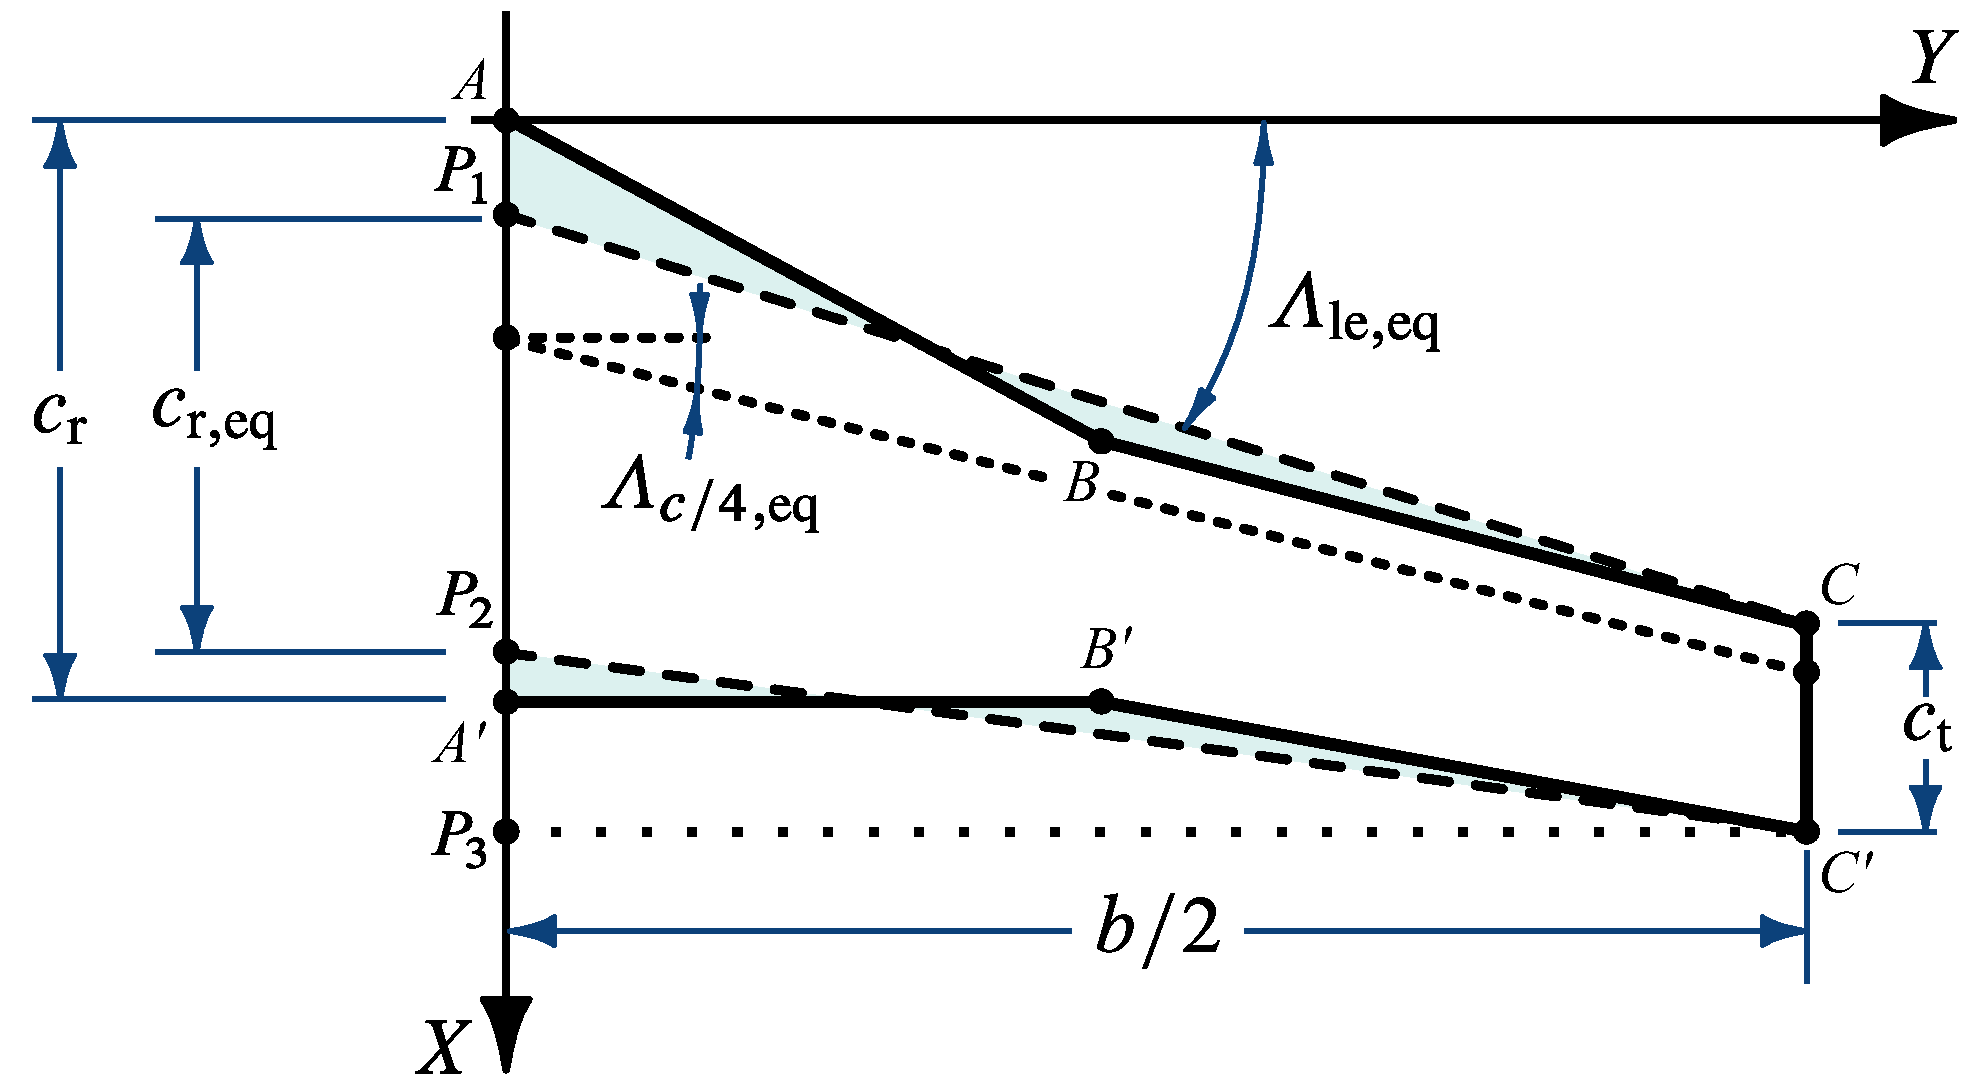
\includegraphics[width=0.78\textwidth]{images/equivalent_wing.pdf}%
%  \caption{\finalhyphendemerits=1000
%           Ala a bordi d'attacco e d'uscita non rettilinei ed ala equivalente a bordi dritti.}
%  \label{fig:Equivalent:Wing:Planform:Defs}%
%\end%
%    %{figure}%
%    {SCfigure}%
%
%\EnlargedFigure% needs two latex passes
%    {t}% #1: t, b, p
%    {images/airfoil_geometry}% #2: the image file included by \includegraphics
%    {width=1.0\textwidth}% #3: option list to pass to \includegraphics, e.g. width=\linewidth,rotate=0
%    {\finalhyphendemerits=1000
%      Alcune caratteristiche geometriche di un profilo alare.}% #4: the caption text
%    {fig:Aero:Profilo:Geometria}% #5: the label
\EnlargedFigureX% needs two latex passes
  {p}% #1: t, b, p
  {%
    \centering
    \begin{tabular}{@{}c@{}}
      \subfloat%\subfigure
          [%
          ]%
          {\label{fig:Wing:DalphaZeroLift:Roskam:Plots:A}%
		      \includegraphics%
		        %[width=0.52\textwidth]%
		        % [height=5.5cm]%
		        [width=0.52\textwidth]%
		        {images/plot_Dalpha0_over_epsT_lam0.pdf}%
          }%
      \\
      \subfloat%\subfigure
          [%
          ]%
          {\label{fig:Wing:DalphaZeroLift:Roskam:Plots:B}%
		      \includegraphics%
		        %[width=0.52\textwidth]%
		        % [height=5.5cm]%
		        [width=0.52\textwidth]%
		        {images/plot_Dalpha0_over_epsT_lam05.pdf}%
          }%
      \\
      \subfloat%\subfigure
          [%            
          ]%
          {\label{fig:Wing:DalphaZeroLift:Roskam:Plots:C}%
		      \includegraphics%
		        %[width=0.52\textwidth]%
		        % [height=5.5cm]%
		        [width=0.52\textwidth]%
		        {images/plot_Dalpha0_over_epsT_lam1.pdf}%
          }%
    \end{tabular}
  }% #2: the image file included by \includegraphics
  {\finalhyphendemerits=1000
     Fattore di correzione \smash{$\big(\upDelta\alpha_{0L}/\epsilon_\mathrm{t}\big)$} 
     per il calcolo dell'angolo di portanza nulla di un'ala finita $\alpha_{0L}$.%
  }% #3: the caption text
  {fig:Wing:DalphaZeroLift:Roskam:Plots}%% #4: the label
%
%-----------------------------------------------------------------------------------------------

%-----------------------------------------------------------------------------------------------
\begin%
  %{figure}
  {SCfigure}[1.9]%
  [t]%[H]%[!htbp]
  %\centering
  %\checkoddpage
  %\centering
  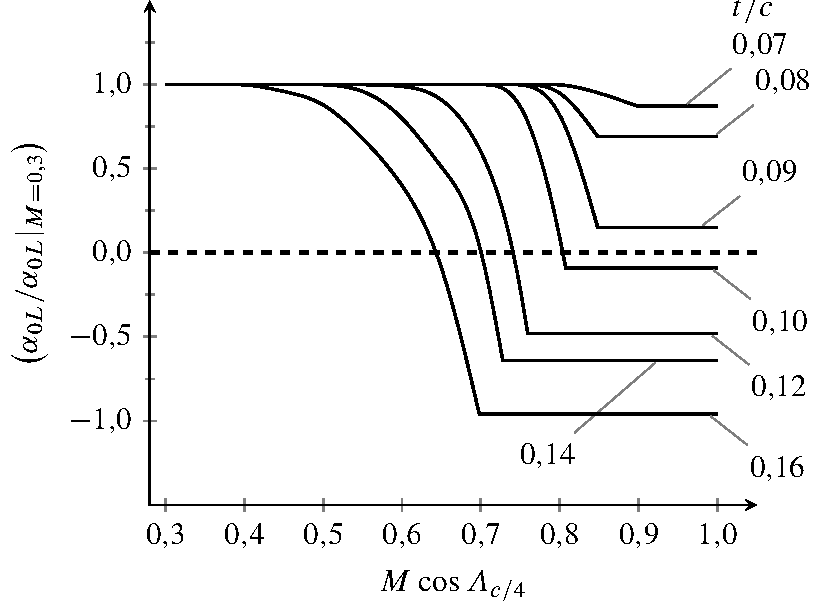
\includegraphics[width=0.65\textwidth]{images/plot_alpha0_PrandtlGlauert_scale.pdf}%
  \caption{\finalhyphendemerits=1000
           Fattore di correzione 
           \smash{$\big(\alpha_{0L}\mathlarger{/}\alpha_{0L}|_{\Mach=\num[round-precision=1]{0.3}}\big)$}
           che incorpora gli effetti della comprimibilità per il calcolo dell'angolo di portanza nulla 
           di un'ala finita $\alpha_{0L}$.}
  \label{fig:Alpha:Zero:Lift:PrandtlGlauert:Scale:Plots}%
\end%
    %{figure}%
    {SCfigure}%
%
%\EnlargedFigure% needs two latex passes
%    {t}% #1: t, b, p
%    {images/airfoil_geometry}% #2: the image file included by \includegraphics
%    {width=1.0\textwidth}% #3: option list to pass to \includegraphics, e.g. width=\linewidth,rotate=0
%    {\finalhyphendemerits=1000
%      Alcune caratteristiche geometriche di un profilo alare.}% #4: the caption text
%    {fig:Aero:Profilo:Geometria}% #5: the label
%\EnlargedFigureX% needs two latex passes
%  {t}% #1: t, b, p
%  {%
%    \makebox[\textwidth][c]{%
%    \includegraphics%
%      %[width=0.52\textwidth]%
%      % [height=5.5cm]%
%      [width=0.485\textwidth]%
%      {images/airfoil_Re_effect_polar.pdf}%
%    %\rule{8mm}{0pt}% <-- SPACER
%    \hfill
%    \raisebox{-0.6mm}[0pt][0pt]{%
%    \includegraphics%
%      %[width=0.52\textwidth]%
%      % [height=5.5cm]%
%      [width=0.485\textwidth]%
%      {images/airfoil_Re_effect_alpha_Cl.pdf}
%    }% end-of-raisebox
%    }% end-of-makebox
%  }% #2: the image file included by \includegraphics
%  {\finalhyphendemerits=1000
%    Influenza del numero di Reynolds, $\Reynolds_{\infty}=V_{\!\infty}c/\nu_{\infty}$,
%           sulla polare e sulla curva di portanza di un profilo NACA 64-212.%
%  }% #3: the caption text
%  {fig:Airfoil:Reynolds:Effects}%% #4: the label
%
%-----------------------------------------------------------------------------------------------
%
%--END-EXERCISE:wing_alpha_zero_lift_2
%===============================================================================================


%=BEGING-EX=================================================================================================
%
%
\begin{myExerciseX}{Angolo di portanza nulla di un'ala finita (metodo grafico)}{\ding{46}\ \myIconGraph\ }% \ \Keyboard\ %
\label{exercise:Wing:Alpha:Zero:Lift:B}
%
\noindent
Con il metodo grafico e per la stessa ala dell'esempio~\ref{example:Wing:Alpha:Zero:Lift:B}
calcolare l'angolo di portanza nulla $\alpha_{0L}$
ai seguenti numeri di Mach di volo:
$M_1=\num[round-precision=1]{0.3}$, 
$M_2=\num[round-precision=1]{0.5}$, 
$M_3=\num[round-precision=1]{0.6}$.

\end{myExerciseX}
%
%=END-EX=====================================================================================================

%=BEGING-ES==================================================================================================
%
\def\mySpanWingMT{10.600000}
\def\mySpanWingIMT{6.360000}
\def\mySpanWingIIMT{4.240000}
\def\myChordRootWingMT{1.440000}
\def\myChordRootWingIMT{1.440000}
\def\myChordRootWingIIMT{1.440000}
\def\myChordTipWingMT{0.860000}
\def\myChordTipWingIMT{1.440000}
\def\myChordTipWingIIMT{0.860000}
\def\mySweepLEWingIIDEG{0.000000}
\def\myCoeffAChordWingI{0.000000}
\def\myCoeffBChordWingIMT{1.440000}
\def\myCoeffAChordWingII{-0.273585}
\def\myCoeffBChordWingIIMT{1.440000}
\def\myAlphaZeroLiftRootWingIDEG{-2.500000}
\def\myAlphaZeroLiftTipWingIDEG{-2.500000}
\def\myAlphaZeroLiftRootWingIRAD{-0.043633}
\def\myAlphaZeroLiftTipWingIRAD{-0.043633}
\def\myAlphaZeroLiftRootWingIIDEG{-2.500000}
\def\myAlphaZeroLiftTipWingIIDEG{-1.000000}
\def\myAlphaZeroLiftRootWingIIRAD{-0.043633}
\def\myAlphaZeroLiftTipWingIIRAD{-0.017453}
\def\myTaperRatioWingI{1.000000}
\def\myTaperRatioWingII{0.597222}
\def\myTwistWingIDEG{0.000000}
\def\myTwistWingIRAD{0.000000}
\def\myTwistWingIIDEG{-3.000000}
\def\myTwistWingIIRAD{-0.052360}
\def\myAreaWingIMTsquared{9.158400}
\def\myAreaWingIIMTsquared{4.876000}
\def\myAreaWingMTsquared{14.034400}
\def\myCoeffAAeroTwistWingIRADMT{0.000000}
\def\myCoeffBAeroTwistWingIRAD{-0.043633}
\def\myCoeffAAeroTwistWingIIRADMT{0.012349}
\def\myCoeffBAeroTwistWingIIRAD{-0.043633}
\def\myCoeffATwistWingIRADMT{0.000000}
\def\myCoeffATwistWingIIRADMT{-0.024698}
\def\myCoeffBTwistWingIRAD{0.000000}
\def\myCoeffBTwistWingIIRAD{0.000000}
\def\myAlphaZeroLiftWingIRAD{-0.028653}
\def\myAlphaZeroLiftWingIDEG{-1.641680}
\def\myAlphaZeroLiftWingIIRAD{0.008329}
\def\myAlphaZeroLiftWingIIDEG{0.477233}
\def\myAlphaZeroLiftWingRAD{-0.020323}
\def\myAlphaZeroLiftWingDEG{-1.164447}

%
\begin{myExampleX}{Gradiente di portanza di un'ala finita}{\ding{46}}% \ \Keyboard\ %
\label{example:Wing:CLAlpha:A}
%
\noindent
È assegnata un'ala finita a bordi dritti e a freccia nulla, cioè con angolo di freccia della linea 
dei fuochi $\Lambda_{c/4}=\SI[round-precision=0]{\mySweepQuarterChordWingDEG}{\degree}$.
Le rimanenti caratteristiche della superficie portante sono le seguenti:

\smallskip
\noindent
\adjustbox{left=\textwidth}{%
  \adjustbox{right=0.39\textwidth}{%
    \emph{corde}:
  }\rule{0.5em}{0pt}% --> SPACER
  \adjustbox{left=0.59\textwidth}{%
    $c_\mathrm{r}=\SI[round-precision=2]{\myChordRootWingMT}{\metre}$,
    $c_\mathrm{t}=\SI[round-precision=2]{\myChordTipWingMT}{\metre}$,
    $\lambda = \SI[round-precision=2]{\myTaperRatioWing}{}$,
  }%
}

\smallskip
\noindent
\adjustbox{left=\textwidth}{%
  \adjustbox{right=0.39\textwidth}{%
    \emph{apertura e superficie}:
  }\rule{0.5em}{0pt}% --> SPACER
  \adjustbox{left=0.59\textwidth}{%
    $b=\SI[round-precision=2]{\mySpanWingMT}{\metre}$,
    $S=\SI[round-precision=2]{\myAreaWingMTsquared}{\meter^2}$,
    $\AR = \SI[round-precision=2]{\myAspectRatioWing}{}$,
  }%
}

\smallskip
\noindent
\adjustbox{left=\textwidth}{%
  \adjustbox{right=0.39\textwidth}{%
    \emph{gradienti $C_{\ell_\mathlarger{\alpha}}$ di profilo}:
  }\rule{0.5em}{0pt}% --> SPACER
  \adjustbox{left=0.59\textwidth}{%
    $C_{\ell_\mathlarger{\alpha},\mathrm{r}}=\SI[round-precision=2]{\myCLAlphaRootWingRAD}{\radian^{-1}}$,
    $C_{\ell_\mathlarger{\alpha},\mathrm{t}}=\SI[round-precision=2]{\myCLAlphaTipWingRAD}{\radian^{-1}}$,
  }%
}

\smallskip
Per l'ala assegnata si vuole calcolare il gradiente \smash{$C_{L_\mathlarger{\alpha}}$}.

\medskip
Se si assumono le seguenti leggi lineari
\[
c \big( Y \big) = A_c \, Y + B_c 
\qquad
C_{\ell_\mathlarger{\alpha}} \big( Y \big) = A_{C_{\ell_\alpha}} \, Y + B_{C_{\ell_\alpha}}
\]
si ha, per quanto riguarda la legge delle corde di sezione
\[
A_c
  = \frac{c_\mathrm{t} - c_\mathrm{r}}{b/2}
  = 
    2 \frac{
      \SI[round-precision=2]{\myChordTipWingMT}{\metre} - \SI[round-precision=2]{\myChordRootWingMT}{\metre}
    }{
      \SI[round-precision=2]{\mySpanWingMT}{\metre}
    }
  = \mathunderline{mydarkblue}{ \SI[round-precision=3]{\myCoeffAChordWing}{} }
\]
\[
B_c
  = c_\mathrm{r}
  = \mathunderline{mydarkblue}{ \SI[round-precision=2]{\myCoeffBChordWingMT}{\metre} }
\]
dunque
\[
c \big( Y \big) = A_c \, Y + B_c
  = \SI[round-precision=3]{\myCoeffAChordWing}{} \, Y
    + \SI[round-precision=2]{\myCoeffBChordWingMT}{\metre}
\]
Analogamente, per la legge dei gradienti del coefficiente di portanza di sezione
\[
\begin{split}
A_{C_{\ell_\alpha}}
  & {}= \frac{C_{\ell_\mathlarger{\alpha},\mathrm{t}} - C_{\ell_\mathlarger{\alpha},\mathrm{r}}}{b/2}
  = 
    2 \frac{
      \SI[round-precision=2]{\myCLAlphaTipWingRAD}{\radian^{-1}} 
      - \SI[round-precision=2]{\myCLAlphaRootWingRAD}{\radian^{-1}}
    }{
      \SI[round-precision=2]{\mySpanWingMT}{\metre}
    }
\\
  & {}= 
    \mathunderline{mydarkblue}{ 
      \SI[round-precision=5]{\myCoeffAClalphaWingRADMT}{\big(\radian\,\metre\big)^{-1}} 
    }
  = 
    \mathunderline{mydarkblue}{ 
      \SI[round-precision=7]{\myCoeffAClalphaWingDEGMT}{\big(\deg\,\metre\big)^{-1}} 
    }
\end{split}
\]
\[
B_{C_{\ell_\alpha}}
  = C_{\ell_\mathlarger{\alpha},\mathrm{r}}
  = \mathunderline{mydarkblue}{ \SI[round-precision=3]{\myCoeffBClalphaWingRAD}{\radian^{-1}} }
\]
cioè
\[
C_{\ell_\mathlarger{\alpha}} \big( Y \big) = A_{C_{\ell_\alpha}} \, Y + B_{C_{\ell_\alpha}}
  = \SI[round-precision=5]{\myCoeffAClalphaWingRADMT}{\big(\radian\,\metre\big)^{-1}} \, Y
    + \SI[round-precision=3]{\myCoeffBClalphaWingRAD}{\radian^{-1}}
\]

Le leggi ricavate sopra permettono di calcolare il gradiente medio
\begin{multline}
\nonumber
\bar{C}_{\ell_\mathlarger{\alpha}}
  = \frac{2}{S} \int_0^{b/2} 
      c\big(Y\big) \, C_{\ell_\mathlarger{\alpha}} \big(Y\big) \diff{Y}
\\
  = \frac{2}{ \SI[round-precision=2]{\myAreaWingMTsquared}{\metre^{2}} } 
    \int_0^{ \calcSI[round-precision=1,fixed-exponent=0,scientific-notation=fixed]{0.5*\mySpanWingMT}{\metre} } 
    \big[
      \SI[round-precision=5]{\myCoeffAClalphaWingRADMT}{\big(\radian\,\metre\big)^{-1}} \, Y
      + \SI[round-precision=3]{\myCoeffBClalphaWingRAD}{\radian^{-1}}
    \big]
    \rule{5em}{0pt}% <-- SPACER
\\
    \rule{5em}{0pt}% <-- SPACER
    \cdot \big[
      \SI[round-precision=3]{\myCoeffAChordWing}{} \, Y
      + \SI[round-precision=2]{\myCoeffBChordWingMT}{\metre}
    \big]
    \diff{Y}
\\
  = \mathunderline{mydarkblue}{ \SI[round-precision=3]{\myCLAlphaMeanWingRAD}{\radian^{-1}} }
  = \mathunderline{mydarkblue}{ \SI[round-precision=4]{\myCLAlphaMeanWingDEG}{\deg^{-1}} }
\end{multline}
Esso può essere utilizzato per il calcolo del gradiente di portanza dell'ala finita
\[
C_{L_\mathlarger{\alpha}}
  = 
    \frac{
      \bar{C}_{\ell_\mathlarger{\alpha}}
    }{
      1 + \dfrac{\bar{C}_{\ell_\mathlarger{\alpha}}}{\pi \AR \, e_\Wing}
    }
  =
    \frac{
      \SI[round-precision=3]{\myCLAlphaMeanWingRAD}{\radian^{-1}}
    }{
      1 + 
        \dfrac{ \SI[round-precision=3]{\myCLAlphaMeanWingRAD}{\radian^{-1}} }{
          \num[round-precision=2]{3.14} 
          \cdot \SI[round-precision=2]{\myAspectRatioWing}{}
          \cdot \SI[round-precision=2]{\myInducedDragFactorWing}{}
        }
    }
  = \mathunderline{mydarkblue}{ \SI[round-precision=3]{\myCLAlphaWingRAD}{\radian^{-1}} }
  = \mathunderline{mydarkblue}{ \SI[round-precision=4]{\myCLAlphaWingDEG}{\deg^{-1}} }
\]

\end{myExampleX}
%
%=END-ES=====================================================================================================

%=BEGING-ES==================================================================================================
%
%\input{exercises/wing_CLAlpha_2/data_a.tex}
%
\begin{myExampleX}{Gradiente di portanza di un'ala finita. Effetto dell'allungamento}{\ding{46}}% \ \Keyboard\ %
\label{example:Wing:CLAlpha:B}
%
\noindent
Si vuole calcolare il gradiente \smash{$C_{L_\mathlarger{\alpha}}$}
di un'ala simile a quella dell'esempio~\ref{example:Wing:CLAlpha:A}
verificando l'effetto della variazione di allungamento
alare.

%-------------------------------------------------
\input{exercises/wing_CLAlpha_2/data_a.tex}
\let\mySpanWingAMT\mySpanWingMT
\let\myAreaWingAMTsquared\myAreaWingMTsquared
\let\myAspectRatioWingA\myAspectRatioWing
\let\myCLAlphaMeanWingARAD\myCLAlphaMeanWingRAD
\let\myCLAlphaMeanWingADEG\myCLAlphaMeanWingDEG
\let\myCLAlphaWingARAD\myCLAlphaWingRAD
\let\myCLAlphaWingADEG\myCLAlphaWingDEG
%-------------------------------------------------
Per l'ala di riferimento si ha:

\smallskip
\noindent
\adjustbox{center=\textwidth}{%
$b=\SI[round-precision=2]{\mySpanWingAMT}{\meter}$,
$\AR=\SI[round-precision=2]{\myAspectRatioWingA}{}$,
$S=\SI[round-precision=2]{\myAreaWingAMTsquared}{\metre^2}$,
\smash{$\bar{C}_{\ell_\mathlarger{\alpha}}=\SI[round-precision=3]{\myCLAlphaMeanWingRAD}{\radian^{-1}}$}
}

\smallskip
\noindent
\adjustbox{center=\textwidth}{%
$C_{L_\mathlarger{\alpha}}
  =\mathunderline{mydarkblue}{ \SI[round-precision=2]{\myCLAlphaWingARAD}{\radian^{-1}} }
  =\mathunderline{mydarkblue}{ \SI[round-precision=3]{\myCLAlphaWingADEG}{\deg^{-1}} }
$
}

\smallskip
%-------------------------------------------------
\def\mySpanWingMT{21.440000}
\def\myMach{0.700000}
\def\myAspectRatioWing{5.687003}
\def\myChordRootWingMT{5.200000}
\def\myChordTipWingMT{2.340000}
\def\myTaperRatioWing{0.450000}
\def\myAreaWingMTsquared{80.828800}
\def\myCoeffAChordWing{-0.266791}
\def\myCoeffBChordWingMT{5.200000}
\def\myCLAlphaRootWingRAD{6.150000}
\def\myCLAlphaTipWingRAD{6.050000}
\def\myCoeffAClalphaWingRADMT{-0.009328}
\def\myCoeffAClalphaWingDEGMT{-0.000163}
\def\myCoeffBClalphaWingRAD{6.150000}
\def\mySweepQuarterChordWingDEG{0.000000}
\def\mySweepQuarterChordWingRAD{0.000000}
\def\myCLAlphaMeanWingRAD{6.106322}
\def\myCLAlphaMeanWingDEG{0.106575}
\def\myInducedDragFactorWing{0.900000}
\def\myCLAlphaWingRAD{4.425656}
\def\myCLAlphaWingDEG{0.077242}

\let\mySpanWingBMT\mySpanWingMT
\let\myAreaWingBMTsquared\myAreaWingMTsquared
\let\myAspectRatioWingB\myAspectRatioWing
\let\myCLAlphaMeanWingBRAD\myCLAlphaMeanWingRAD
\let\myCLAlphaMeanWingBDEG\myCLAlphaMeanWingDEG
\let\myCLAlphaWingBRAD\myCLAlphaWingRAD
\let\myCLAlphaWingBDEG\myCLAlphaWingDEG
%-------------------------------------------------
Per un'ala di pari corda di radice e rapporto di rastremazione,
ma di apertura $b'$ diminuita del $20\%$ rispetto alla $b$ si ha:

\smallskip
\noindent
\adjustbox{center=\textwidth}{%
$b'=\SI[round-precision=2]{\mySpanWingBMT}{\meter}$,
$\AR'=\SI[round-precision=2]{\myAspectRatioWingB}{}$,
$S'=\SI[round-precision=2]{\myAreaWingBMTsquared}{\metre^2}$,
\smash{$\bar{C}_{\ell_\mathlarger{\alpha}}'=\SI[round-precision=4]{\myCLAlphaMeanWingRAD}{\radian^{-1}}$}
}

\smallskip
\noindent
\adjustbox{center=\textwidth}{%
$C_{L_\mathlarger{\alpha}}'
  =\mathunderline{mydarkblue}{ \SI[round-precision=2]{\myCLAlphaWingBRAD}{\radian^{-1}} }
  =\mathunderline{mydarkblue}{ \SI[round-precision=3]{\myCLAlphaWingBDEG}{\deg^{-1}} }
$
}

\smallskip
%-------------------------------------------------
\def\mySpanWingMT{32.160000}
\def\myMach{0.700000}
\def\myAspectRatioWing{8.530504}
\def\myChordRootWingMT{5.200000}
\def\myChordTipWingMT{2.340000}
\def\myTaperRatioWing{0.450000}
\def\myAreaWingMTsquared{121.243200}
\def\myCoeffAChordWing{-0.177861}
\def\myCoeffBChordWingMT{5.200000}
\def\myCLAlphaRootWingRAD{6.150000}
\def\myCLAlphaTipWingRAD{6.050000}
\def\myCoeffAClalphaWingRADMT{-0.006219}
\def\myCoeffAClalphaWingDEGMT{-0.000109}
\def\myCoeffBClalphaWingRAD{6.150000}
\def\mySweepQuarterChordWingDEG{0.000000}
\def\mySweepQuarterChordWingRAD{0.000000}
\def\myCLAlphaMeanWingRAD{6.106322}
\def\myCLAlphaMeanWingDEG{0.106575}
\def\myInducedDragFactorWing{0.900000}
\def\myCLAlphaWingRAD{4.872699}
\def\myCLAlphaWingDEG{0.085045}

\let\mySpanWingCMT\mySpanWingMT
\let\myAreaWingCMTsquared\myAreaWingMTsquared
\let\myAspectRatioWingC\myAspectRatioWing
\let\myCLAlphaMeanWingCRAD\myCLAlphaMeanWingRAD
\let\myCLAlphaMeanWingCDEG\myCLAlphaMeanWingDEG
\let\myCLAlphaWingCRAD\myCLAlphaWingRAD
\let\myCLAlphaWingCDEG\myCLAlphaWingDEG
%-------------------------------------------------
Analogamente, per un'ala di apertura $b''$ aumentata del $20\%$ rispetto alla $b$ si ha:

\smallskip
\noindent
\adjustbox{center=\textwidth}{%
$b''=\SI[round-precision=2]{\mySpanWingCMT}{\meter}$,
$\AR''=\SI[round-precision=2]{\myAspectRatioWingC}{}$,
$S''=\SI[round-precision=2]{\myAreaWingCMTsquared}{\metre^2}$,
\smash{$\bar{C}_{\ell_\mathlarger{\alpha}}''=\SI[round-precision=4]{\myCLAlphaMeanWingRAD}{\radian^{-1}}$}
}

\smallskip
\noindent
\adjustbox{center=\textwidth}{%
$C_{L_\mathlarger{\alpha}}''
  =\mathunderline{mydarkblue}{ \SI[round-precision=2]{\myCLAlphaWingCRAD}{\radian^{-1}} }
  =\mathunderline{mydarkblue}{ \SI[round-precision=3]{\myCLAlphaWingCDEG}{\deg^{-1}} }
$
}

\medskip
I valori dei gradienti $C_{L_\mathlarger{\alpha}}'$ e $C_{L_\mathlarger{\alpha}}''$
sono calcolati applicando il procedimento dell'esempio~\ref{example:Wing:CLAlpha:A}.
Si osserva che per un allungamento via via crescente
($\AR' < \AR < \AR''$) cresce il gradiente della retta di portanza dell'ala
($C_{L_\mathlarger{\alpha}}' < C_{L_\mathlarger{\alpha}} < C_{L_\mathlarger{\alpha}}''$).

Si veda la figura~\ref{fig:CLAlpha:Wing:Planforms:B} per una conferma grafica dei risultati precedenti.

\end{myExampleX}
%
%=END-ES=====================================================================================================


%-----------------------------------------------------------------------------------------------
\begin%
  %{figure}
  {SCfigure}[1.9]%
  [t]%[H]%[!htbp]
  %\centering
  %\checkoddpage
  %\centering
    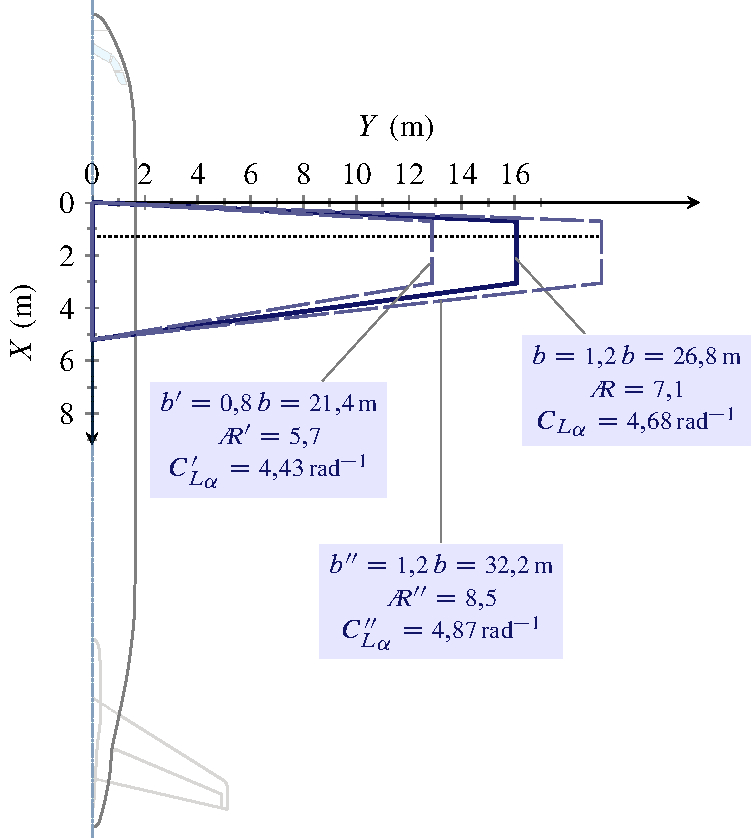
\includegraphics[width=0.70\textwidth]{exercises/wing_CLAlpha_2/wing_planforms_drawing.pdf}%
  \caption{\finalhyphendemerits=1000
           Forme in pianta al variare dell'apertura, a parità di corde di radice e di estremità.}
  \label{fig:CLAlpha:Wing:Planforms:B}%
\end%
    %{figure}%
    {SCfigure}%
%
%\EnlargedFigure% needs two latex passes
%    {t}% #1: t, b, p
%    {images/airfoil_geometry}% #2: the image file included by \includegraphics
%    {width=1.0\textwidth}% #3: option list to pass to \includegraphics, e.g. width=\linewidth,rotate=0
%    {\finalhyphendemerits=1000
%      Alcune caratteristiche geometriche di un profilo alare.}% #4: the caption text
%    {fig:Aero:Profilo:Geometria}% #5: the label
%\EnlargedFigureX% needs two latex passes
%  {t}% #1: t, b, p
%  {%
%    \makebox[\textwidth][c]{%
%    \includegraphics%
%      %[width=0.52\textwidth]%
%      % [height=5.5cm]%
%      [width=0.485\textwidth]%
%      {images/airfoil_Re_effect_polar.pdf}%
%    %\rule{8mm}{0pt}% <-- SPACER
%    \hfill
%    \raisebox{-0.6mm}[0pt][0pt]{%
%    \includegraphics%
%      %[width=0.52\textwidth]%
%      % [height=5.5cm]%
%      [width=0.485\textwidth]%
%      {images/airfoil_Re_effect_alpha_Cl.pdf}
%    }% end-of-raisebox
%    }% end-of-makebox
%  }% #2: the image file included by \includegraphics
%  {\finalhyphendemerits=1000
%    Influenza del numero di Reynolds, $\Reynolds_{\infty}=V_{\!\infty}c/\nu_{\infty}$,
%           sulla polare e sulla curva di portanza di un profilo NACA 64-212.%
%  }% #3: the caption text
%  {fig:Airfoil:Reynolds:Effects}%% #4: the label
%
%-----------------------------------------------------------------------------------------------

%=BEGING-ES==================================================================================================
%
\def\mySpanWingMT{10.600000}
\def\mySpanWingIMT{6.360000}
\def\mySpanWingIIMT{4.240000}
\def\myChordRootWingMT{1.440000}
\def\myChordRootWingIMT{1.440000}
\def\myChordRootWingIIMT{1.440000}
\def\myChordTipWingMT{0.860000}
\def\myChordTipWingIMT{1.440000}
\def\myChordTipWingIIMT{0.860000}
\def\mySweepLEWingIIDEG{0.000000}
\def\myCoeffAChordWingI{0.000000}
\def\myCoeffBChordWingIMT{1.440000}
\def\myCoeffAChordWingII{-0.273585}
\def\myCoeffBChordWingIIMT{1.440000}
\def\myAlphaZeroLiftRootWingIDEG{-2.500000}
\def\myAlphaZeroLiftTipWingIDEG{-2.500000}
\def\myAlphaZeroLiftRootWingIRAD{-0.043633}
\def\myAlphaZeroLiftTipWingIRAD{-0.043633}
\def\myAlphaZeroLiftRootWingIIDEG{-2.500000}
\def\myAlphaZeroLiftTipWingIIDEG{-1.000000}
\def\myAlphaZeroLiftRootWingIIRAD{-0.043633}
\def\myAlphaZeroLiftTipWingIIRAD{-0.017453}
\def\myTaperRatioWingI{1.000000}
\def\myTaperRatioWingII{0.597222}
\def\myTwistWingIDEG{0.000000}
\def\myTwistWingIRAD{0.000000}
\def\myTwistWingIIDEG{-3.000000}
\def\myTwistWingIIRAD{-0.052360}
\def\myAreaWingIMTsquared{9.158400}
\def\myAreaWingIIMTsquared{4.876000}
\def\myAreaWingMTsquared{14.034400}
\def\myCoeffAAeroTwistWingIRADMT{0.000000}
\def\myCoeffBAeroTwistWingIRAD{-0.043633}
\def\myCoeffAAeroTwistWingIIRADMT{0.012349}
\def\myCoeffBAeroTwistWingIIRAD{-0.043633}
\def\myCoeffATwistWingIRADMT{0.000000}
\def\myCoeffATwistWingIIRADMT{-0.024698}
\def\myCoeffBTwistWingIRAD{0.000000}
\def\myCoeffBTwistWingIIRAD{0.000000}
\def\myAlphaZeroLiftWingIRAD{-0.028653}
\def\myAlphaZeroLiftWingIDEG{-1.641680}
\def\myAlphaZeroLiftWingIIRAD{0.008329}
\def\myAlphaZeroLiftWingIIDEG{0.477233}
\def\myAlphaZeroLiftWingRAD{-0.020323}
\def\myAlphaZeroLiftWingDEG{-1.164447}

%
\begin{myExampleX}{Gradiente di portanza di un'ala finita, formula di Polhamus}{\ding{46}}% \ \Keyboard\ %
\label{example:Wing:CLAlpha:C}
%
\noindent
Si vuole calcolare il gradiente \smash{$C_{L_\mathlarger{\alpha}}$} di un'ala finita
a freccia con una formula nota con il nome di \emph{formula di Polhamus}:
\begin{equation}\label{eq:Aero:Polhamus:Formula}
C_{L_{\mathlarger{\alpha}}} = 
   \frac{ 2\pi\AR
   }{
      2 + \SQRT{ 4+ \frac{\AR^2 \big(1-M^2\big)}{k_\mathrm{P}^2}\LEFTRIGHT(){1+\frac{\tan^2\Lambda_{c/2}}{1-M^2}} }
   }
\end{equation}
con
\begin{equation}\label{eq:Aero:K:Polhamus:Formula}
k_\mathrm{P}=\LEFTRIGHT\lcbrace.{
   \begin{array}{ll}
      1+\AR\dfrac{\num[round-precision=2]{1.87}-\num[round-precision=6]{0.000233}\Lambda_\mathrm{le}}{\num[round-precision=0]{100}}
      & \text{se}\, \AR<4
      \\[1em]
      1+\dfrac{
         \big(\num[round-precision=1]{8.2}-\num[round-precision=1]{2.3}\Lambda_\mathrm{le}\big)
         - \AR\big(\num[round-precision=2]{0.22}-\num[round-precision=3]{0.153}\Lambda_\mathrm{le}\big)
         }{\num[round-precision=0]{100}}
      & \text{se}\, \AR \ge 4
   \end{array}
}
\end{equation}
e $\Lambda_\text{le}$ in radianti.
La (\ref{eq:Aero:Polhamus:Formula}) è da ritenersi applicabile per ali finite
aventi
\begin{equation}\label{eq:Aero:Limitations:Polhamus:Formula}
\Lambda_\mathrm{le} < \SI[round-precision=0]{32}{\degree}
\,,\quad
\SI[round-precision=1]{0.4}{} < \lambda \le 1
\,,\quad
3 \le \AR \le 8
\end{equation}
e per un numero di Mach di volo $\Mach < \Mach_\mathrm{cr}$.

Si consideri un'ala con bordi d'attacco e d'uscita rettilinei,
%simile a quella dell'esempio~\ref{example:Wing:Basic:A},
di apertura $b=\SI[round-precision=1]{\mySpanWingMT}{\metre}$,
corda di radice $c_\mathrm{r}=\SI[round-precision=2]{\myChordRootWingMT}{\metre}$,
corda d'estremità $c_\mathrm{t}=\SI[round-precision=2]{\myChordTipWingMT}{\metre}$
e freccia del bordo d'attacco
$\Lambda_\mathrm{le}=\SI[round-precision=1]{\mySweepLEWingDEG}{\deg}$.
Si assuma un numero di Mach di volo $\Mach=\SI[round-precision=1]{\myMach}{}$
e un $\Mach_\mathrm{cr}\simeq\SI[round-precision=2]{\myCriticalMachNumberMACWing}{}$.

Si lascia per esercizio al lettore il compito di verificare che
la forma in pianta assegnata ha
un rapporto di rastremazione
$\lambda=\SI[round-precision=2]{\myTaperRatioWing}{}$,
una superficie alare
$S=\SI[round-precision=1]{\myAreaWingMTsquared}{\metre^2}$,
un allungamento alare
$\AR=\num[round-precision=2]{\myAspectRatioWing}$
e un angolo
$\Lambda_{c/2}=\SI[round-precision=3]{\mySweepHalfChordWingRAD}{\radian}=\SI[round-precision=1]{\mySweepHalfChordWingDEG}{\deg}$.

I dati dell'ala sono tali da soddisfare le condizioni (\ref{eq:Aero:Limitations:Polhamus:Formula})
e, sostituiti nelle (\ref{eq:Aero:Polhamus:Formula})-(\ref{eq:Aero:K:Polhamus:Formula}), 
permettono di ricavare
\[
k_\mathrm{P} 
  =
    1+\dfrac{
      \big(
        \num[round-precision=1]{8.2}
        -\num[round-precision=1]{2.3}
        \cdot \SI[round-precision=3]{\mySweepLEWingRAD}{\radian}
      \big)
      - \num[round-precision=2]{\myAspectRatioWing}\,
      \big(
        \num[round-precision=2]{0.22}-\num[round-precision=3]{0.153}
        \cdot \SI[round-precision=3]{\mySweepLEWingRAD}{\radian}
      \big)
    }{\num[round-precision=0]{100}}
  = \mathunderline{mydarkblue}{ \SI[round-precision=2]{\myKPolhamus}{} }
\]
e
\[
\begin{split}
C_{L_{\mathlarger{\alpha}}} 
  & {}= 
   \frac{ 2\pi\AR
   }{
      2 + \SQRT{ 4+ \frac{\AR^2 \big(1-M^2\big)}{k_\mathrm{P}^2}\LEFTRIGHT(){1+\frac{\tan^2\Lambda_{c/2}}{1-M^2}} }
   }
\\[10pt]
  & {}= 
  \frac{ \num[round-precision=3]{6.28} \cdot \num[round-precision=2]{\myAspectRatioWing}
   }{
      2 + \SQRT{ 4+ 
      \frac{
        \num[round-precision=2]{\myAspectRatioWing}^2 \big( 1-\num[round-precision=2]{\myMach}^2 \big)
      }{
        \SI[round-precision=2]{\myKPolhamus}{}^2}
        \LEFTRIGHT(){ 1 +
          \frac{
            \tan^2 \SI[round-precision=3]{\mySweepHalfChordWingRAD}{\radian}
          }{
            1-\num[round-precision=2]{\myMach}^2
          }
        } 
      }
   }
    =\mathunderline{mydarkblue}{ \SI[round-precision=2]{\myCLAlphaWingRAD}{\radian^{-1}} }
    =\mathunderline{mydarkblue}{ \SI[round-precision=3]{\myCLAlphaWingDEG}{\deg^{-1}} }
\end{split}
\]

\end{myExampleX}
%
%=END-ES=====================================================================================================

%-----------------------------------------------------------------------------------------------
%\begin%
%  %{figure}
%  {SCfigure}[1.9]%
%  [t]%[H]%[!htbp]
%  %\centering
%  %\checkoddpage
%  %\centering
%    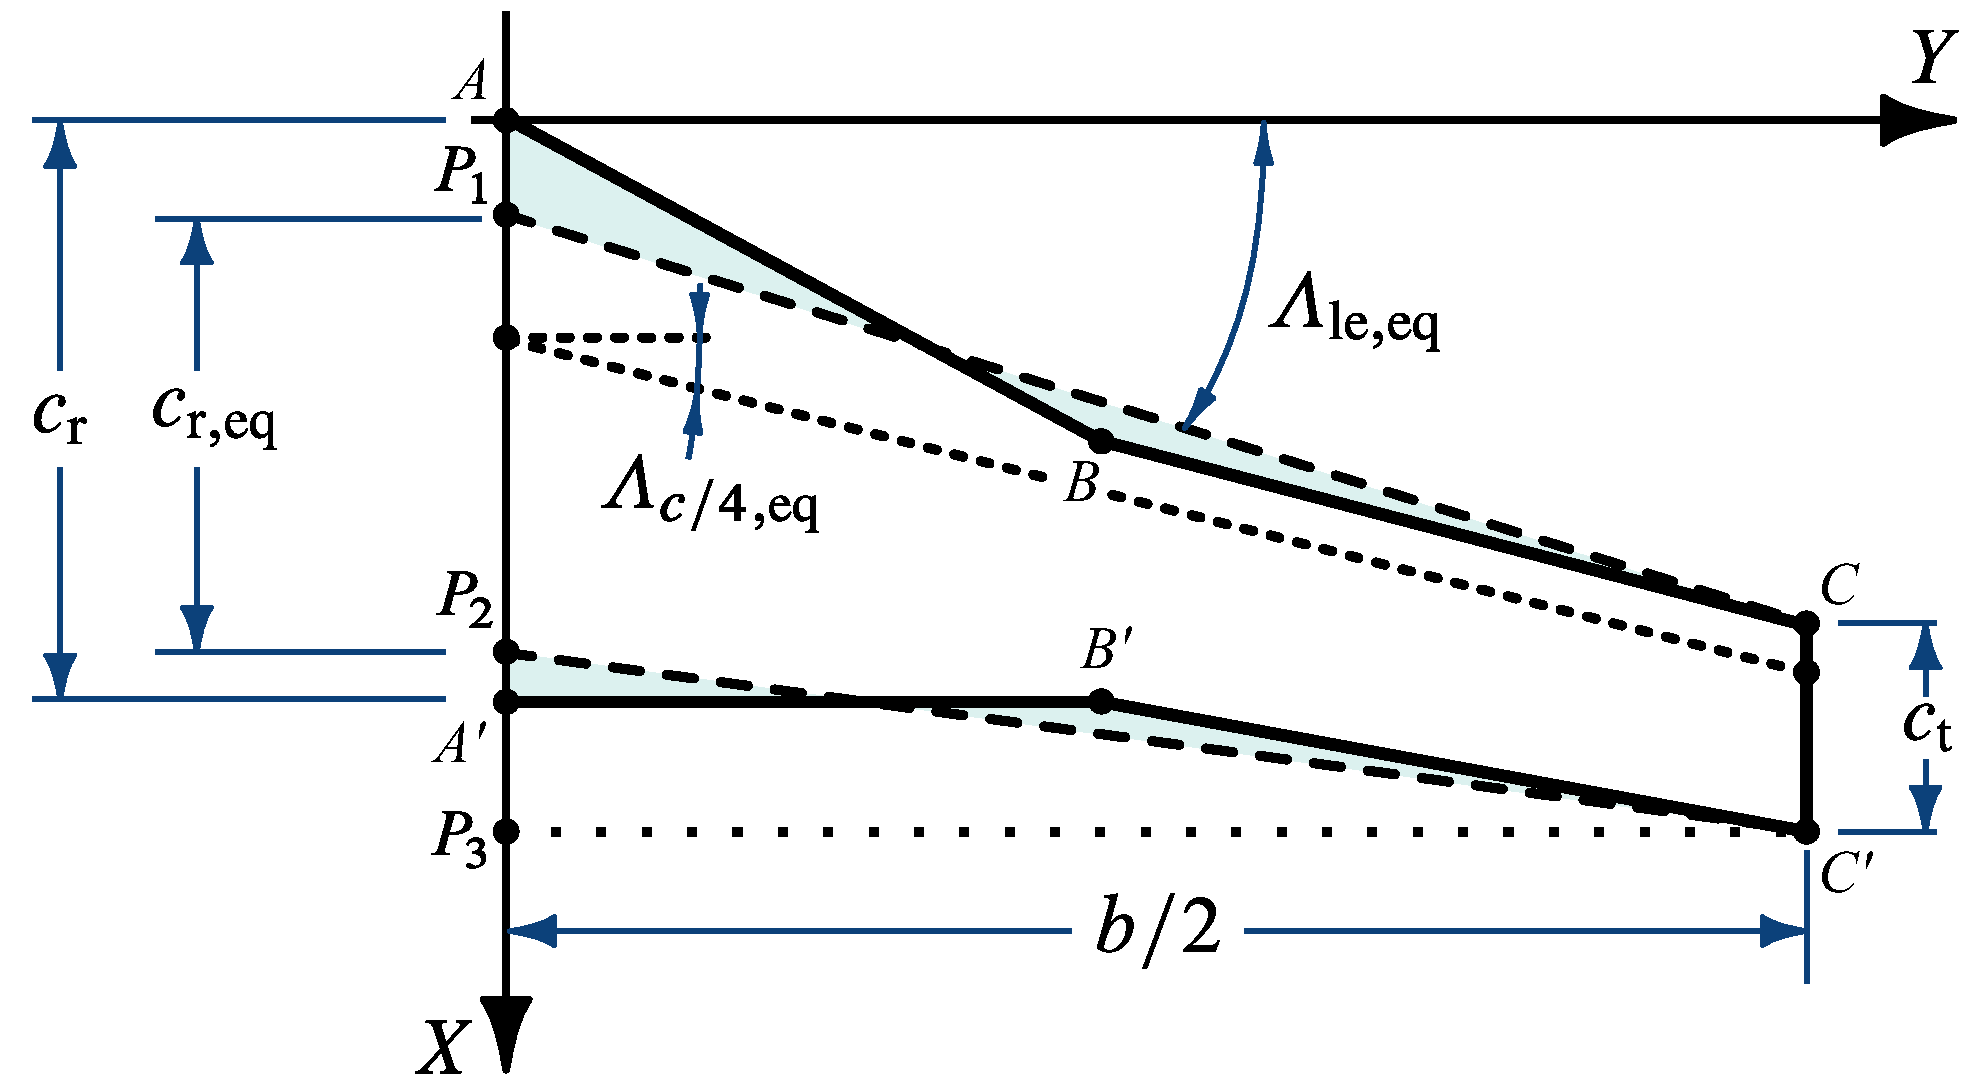
\includegraphics[width=0.78\textwidth]{images/equivalent_wing.pdf}%
%  \caption{\finalhyphendemerits=1000
%           Ala a bordi d'attacco e d'uscita non rettilinei ed ala equivalente a bordi dritti.}
%  \label{fig:Equivalent:Wing:Planform:Defs}%
%\end%
%    %{figure}%
%    {SCfigure}%
%
%\EnlargedFigure% needs two latex passes
%    {t}% #1: t, b, p
%    {images/airfoil_geometry}% #2: the image file included by \includegraphics
%    {width=1.0\textwidth}% #3: option list to pass to \includegraphics, e.g. width=\linewidth,rotate=0
%    {\finalhyphendemerits=1000
%      Alcune caratteristiche geometriche di un profilo alare.}% #4: the caption text
%    {fig:Aero:Profilo:Geometria}% #5: the label
\EnlargedFigureX% needs two latex passes
  {p}% #1: t, b, p
  {%
    \centering
    \begin{tabular}{@{}c@{}}
      \subfloat%\subfigure
          [%
            \smash{$C_{L_\mathlarger{\alpha}}$} al variare di $\Mach$, per
            diversi valori del parametro $\AR$.
          ]%
          {\label{fig:Wing:CLAlpha:Polhamus:Formula:Plots:A}%
		      \includegraphics%
		        %[width=0.52\textwidth]%
		        % [height=5.5cm]%
		        [width=0.45\textwidth]%
		        {images/plot_wing_CLalpha_LamLE15_lam05.pdf}%
          }%
      \\
      \subfloat%\subfigure
          [%
            \smash{$C_{L_\mathlarger{\alpha}}$} al variare di $\Mach$, per
            diversi valori del parametro $\Lambda_\text{le}$.
          ]%
          {\label{fig:Wing:CLAlpha:Polhamus:Formula:Plots:B}%
		      \includegraphics%
		        %[width=0.52\textwidth]%
		        % [height=5.5cm]%
		        [width=0.45\textwidth]%
		        {images/plot_wing_CLalpha_lam05_AR5.pdf}%
          }%
      \\
      \subfloat%\subfigure
          [%
            \smash{$C_{L_\mathlarger{\alpha}}$} al variare di $\Mach$, per
            diversi valori del parametro $\lambda$.
          ]%
          {\label{fig:Wing:CLAlpha:Polhamus:Formula:Plots:C}%
		      \includegraphics%
		        %[width=0.52\textwidth]%
		        % [height=5.5cm]%
		        [width=0.45\textwidth]%
		        {images/plot_wing_CLalpha_LamLE15_AR5.pdf}%
          }%
    \end{tabular}
  }% #2: the image file included by \includegraphics
  {\finalhyphendemerits=1000
     Rappresentazioni grafiche della formula di Polhamus per il calcolo
     del gradiente \smash{$C_{L_\mathlarger{\alpha}}$}.%
  }% #3: the caption text
  {fig:Wing:CLAlpha:Polhamus:Formula:Plots}%% #4: the label
%
%-----------------------------------------------------------------------------------------------

%=BEGING-ES===========================================================================================
%
\def\mySpanWingMT{10.600000}
\def\mySpanWingIMT{6.360000}
\def\mySpanWingIIMT{4.240000}
\def\myChordRootWingMT{1.440000}
\def\myChordRootWingIMT{1.440000}
\def\myChordRootWingIIMT{1.440000}
\def\myChordTipWingMT{0.860000}
\def\myChordTipWingIMT{1.440000}
\def\myChordTipWingIIMT{0.860000}
\def\mySweepLEWingIIDEG{0.000000}
\def\myCoeffAChordWingI{0.000000}
\def\myCoeffBChordWingIMT{1.440000}
\def\myCoeffAChordWingII{-0.273585}
\def\myCoeffBChordWingIIMT{1.440000}
\def\myAlphaZeroLiftRootWingIDEG{-2.500000}
\def\myAlphaZeroLiftTipWingIDEG{-2.500000}
\def\myAlphaZeroLiftRootWingIRAD{-0.043633}
\def\myAlphaZeroLiftTipWingIRAD{-0.043633}
\def\myAlphaZeroLiftRootWingIIDEG{-2.500000}
\def\myAlphaZeroLiftTipWingIIDEG{-1.000000}
\def\myAlphaZeroLiftRootWingIIRAD{-0.043633}
\def\myAlphaZeroLiftTipWingIIRAD{-0.017453}
\def\myTaperRatioWingI{1.000000}
\def\myTaperRatioWingII{0.597222}
\def\myTwistWingIDEG{0.000000}
\def\myTwistWingIRAD{0.000000}
\def\myTwistWingIIDEG{-3.000000}
\def\myTwistWingIIRAD{-0.052360}
\def\myAreaWingIMTsquared{9.158400}
\def\myAreaWingIIMTsquared{4.876000}
\def\myAreaWingMTsquared{14.034400}
\def\myCoeffAAeroTwistWingIRADMT{0.000000}
\def\myCoeffBAeroTwistWingIRAD{-0.043633}
\def\myCoeffAAeroTwistWingIIRADMT{0.012349}
\def\myCoeffBAeroTwistWingIIRAD{-0.043633}
\def\myCoeffATwistWingIRADMT{0.000000}
\def\myCoeffATwistWingIIRADMT{-0.024698}
\def\myCoeffBTwistWingIRAD{0.000000}
\def\myCoeffBTwistWingIIRAD{0.000000}
\def\myAlphaZeroLiftWingIRAD{-0.028653}
\def\myAlphaZeroLiftWingIDEG{-1.641680}
\def\myAlphaZeroLiftWingIIRAD{0.008329}
\def\myAlphaZeroLiftWingIIDEG{0.477233}
\def\myAlphaZeroLiftWingRAD{-0.020323}
\def\myAlphaZeroLiftWingDEG{-1.164447}

%
\begin{myExampleX}{Centro aerodinamico di un'ala a bordi dritti, rastremata, a freccia}{\ding{46}\ \myIconGraph\ }% \ \Keyboard\ %
\label{example:Wing:Aerodynamic:Center:A}
%
\noindent
Si consideri l'ala assegnata nell'esempio~\ref{example:Wing:Basic:A}.
Con l'aiuto dei grafici riportati nelle figure~\ref{fig:Wing:Ac:K:One:Plots},
\ref{fig:Wing:Ac:K:Two:Plots} e~\ref{fig:Wing:Ac:X:AC:From:Apex:Plots}, calcolare
la posizione del centro aerodinamico per un numero di Mach di volo
$\Mach = \SI[round-precision=2]{\myMach}{}$.

\medskip
Dai dati e dalla figura~\ref{fig:Wing:Ac:K:One:Plots}
si legge
\[
\lambda=\SI[round-precision=2]{\myTaperRatioWing}{}
%
%\quad \Longrightarrow \quad
%\quad \begin{array}{@{}c@{}} \myIconGraph \\[-4pt] \Longrightarrow \end{array} \quad
\adjustbox{center=4em}{%
  \adjustbox{lap=\width}{\raisebox{2.2ex}[0pt][0pt]{\myIconGraph}}$\Longrightarrow$%
}
%
K_1
  = \mathunderline{mydarkblue}{ \SI[round-precision=3]{\myKOneACDatcomWing}{} }
\]
dalla figura~\ref{fig:Wing:Ac:K:Two:Plots}
si legge
\[
\Lambda_\mathrm{le} = \SI[round-precision=1]{\mySweepLEWingDEG}{\deg}\;,\;\,
\AR = \SI[round-precision=1]{\myAspectRatioWing}{}\;,\;\,
\lambda=\SI[round-precision=2]{\myTaperRatioWing}{}
%\quad \Longrightarrow \quad
%\quad \begin{array}{@{}c@{}} \myIconGraph \\[-4pt] \Longrightarrow \end{array} \quad
\adjustbox{center=4em}{%
  \adjustbox{lap=\width}{\raisebox{2.2ex}[0pt][0pt]{\myIconGraph}}$\Longrightarrow$%
}
%
K_2 
  = \mathunderline{mydarkblue}{ \SI[round-precision=3]{\myKTwoACDatcomWing}{} }
\]
dalla figura~\ref{fig:Wing:Ac:X:AC:From:Apex:Plots}
si legge
\[
\Lambda_\mathrm{le} = \SI[round-precision=1]{\mySweepLEWingDEG}{\deg}\;,\;\,
\Mach = \SI[round-precision=2]{\myMach}{}\;,\;\,
\AR = \SI[round-precision=1]{\myAspectRatioWing}{}\;,\;\,
\lambda=\SI[round-precision=2]{\myTaperRatioWing}{}
%
%\quad \Longrightarrow \quad
%\quad \begin{array}{@{}c@{}} \myIconGraph \\[-4pt] \Longrightarrow \end{array} \quad
\adjustbox{center=4em}{%
  \adjustbox{lap=\width}{\raisebox{2.2ex}[0pt][0pt]{\myIconGraph}}$\Longrightarrow$%
}
%
\frac{X'_{\mathrm{ac}}}{c_\mathrm{r}}
  = \mathunderline{mydarkblue}{ \SI[round-precision=3]{\myXACOverChordRootDatcomWing}{} }
\]
%
Si ottiene dunque
\[
\frac{x_{\mathrm{ac}}}{\bar{c}} 
  = K_1 \left( \frac{X'_{\mathrm{ac}}}{c_\mathrm{r}} - K_2  \right)
  = \SI[round-precision=3]{\myKOneACDatcomWing}{} \,
    \Big(  
      \SI[round-precision=3]{\myXACOverChordRootDatcomWing}{} 
        - \SI[round-precision=3]{\myKTwoACDatcomWing}{}  
    \Big)
  = \mathunderline{mydarkblue}{ \SI[round-precision=3]{\myXsiACWing}{} } 
\]

La rappresentazione grafica del centro aerodinamico dell'ala assegnata
$(X_\mathrm{ac},0)$ è data dalla figura~\ref{fig:Wing:Aerodynamic:Center:Results:A}.
La posizione del $X_\mathrm{ac}$ è facilmente calcolabile come
\[
\begin{split}
X_\mathrm{ac} & {}= X_{\mathrm{le},\bar{c}} + \left( \frac{x_{\mathrm{ac}}}{\bar{c}} \right) \bar{c}
\\
  & {}=
    \SI[round-precision=2]{\myXMACLEToApexWingMT}{\metre}
      + \SI[round-precision=3]{\myXsiACWing}{}
        \cdot \SI[round-precision=2]{\myMACWingMT}{\metre}
      = \SI[round-precision=2]{\myXMACLEToApexWingMT}{\metre}
        + \calcSI[round-precision=2]{\myXsiACWing*\myMACWingMT}{\metre}
    = \mathunderline{mydarkblue}{ 
      \calcSI[round-precision=2]{\myXMACLEToApexWingMT + \myXsiACWing*\myMACWingMT}{\metre} 
    }%
\end{split}
\]


\end{myExampleX}
%=END-ES===========================================================================================

%-----------------------------------------------------------------------------------------------
\begin%
  %{figure}
  {SCfigure}[1.9]%
  [t]%[H]%[!htbp]
  %\centering
  %\checkoddpage
  %\centering
    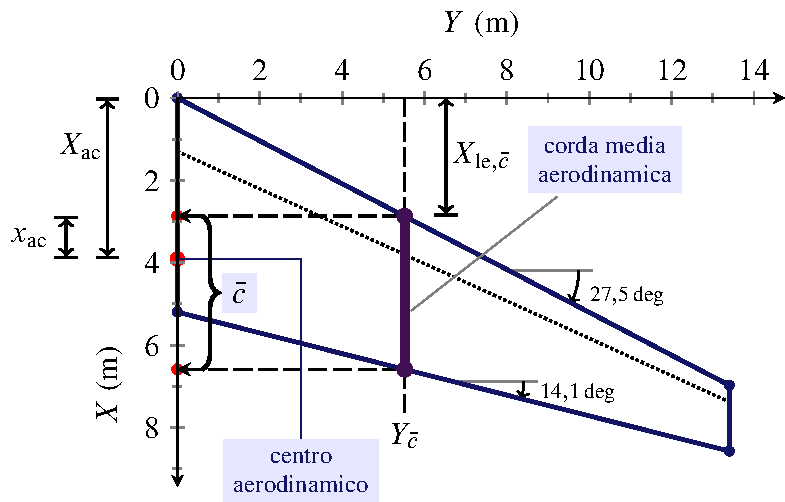
\includegraphics[width=0.70\textwidth]{exercises/wing_ac_1/wing_ac_1_drawing.pdf}%
  \caption{\finalhyphendemerits=1000
           Centro aerodinamico dell'ala assegnata nell'esempio~\ref{example:Wing:Aerodynamic:Center:A}.}
  \label{fig:Wing:Aerodynamic:Center:Results:A}%
\end%
    %{figure}%
    {SCfigure}%
%
%\EnlargedFigure% needs two latex passes
%    {t}% #1: t, b, p
%    {images/airfoil_geometry}% #2: the image file included by \includegraphics
%    {width=1.0\textwidth}% #3: option list to pass to \includegraphics, e.g. width=\linewidth,rotate=0
%    {\finalhyphendemerits=1000
%      Alcune caratteristiche geometriche di un profilo alare.}% #4: the caption text
%    {fig:Aero:Profilo:Geometria}% #5: the label
%\EnlargedFigureX% needs two latex passes
%  {t}% #1: t, b, p
%  {%
%    \makebox[\textwidth][c]{%
%    \includegraphics%
%      %[width=0.52\textwidth]%
%      % [height=5.5cm]%
%      [width=0.485\textwidth]%
%      {images/airfoil_Re_effect_polar.pdf}%
%    %\rule{8mm}{0pt}% <-- SPACER
%    \hfill
%    \raisebox{-0.6mm}[0pt][0pt]{%
%    \includegraphics%
%      %[width=0.52\textwidth]%
%      % [height=5.5cm]%
%      [width=0.485\textwidth]%
%      {images/airfoil_Re_effect_alpha_Cl.pdf}
%    }% end-of-raisebox
%    }% end-of-makebox
%  }% #2: the image file included by \includegraphics
%  {\finalhyphendemerits=1000
%    Influenza del numero di Reynolds, $\Reynolds_{\infty}=V_{\!\infty}c/\nu_{\infty}$,
%           sulla polare e sulla curva di portanza di un profilo NACA 64-212.%
%  }% #3: the caption text
%  {fig:Airfoil:Reynolds:Effects}%% #4: the label
%
%-----------------------------------------------------------------------------------------------


%%=BEGING-ES==================================================================================================
%%
%%\def\mySpanWingMT{10.600000}
\def\mySpanWingIMT{6.360000}
\def\mySpanWingIIMT{4.240000}
\def\myChordRootWingMT{1.440000}
\def\myChordRootWingIMT{1.440000}
\def\myChordRootWingIIMT{1.440000}
\def\myChordTipWingMT{0.860000}
\def\myChordTipWingIMT{1.440000}
\def\myChordTipWingIIMT{0.860000}
\def\mySweepLEWingIIDEG{0.000000}
\def\myCoeffAChordWingI{0.000000}
\def\myCoeffBChordWingIMT{1.440000}
\def\myCoeffAChordWingII{-0.273585}
\def\myCoeffBChordWingIIMT{1.440000}
\def\myAlphaZeroLiftRootWingIDEG{-2.500000}
\def\myAlphaZeroLiftTipWingIDEG{-2.500000}
\def\myAlphaZeroLiftRootWingIRAD{-0.043633}
\def\myAlphaZeroLiftTipWingIRAD{-0.043633}
\def\myAlphaZeroLiftRootWingIIDEG{-2.500000}
\def\myAlphaZeroLiftTipWingIIDEG{-1.000000}
\def\myAlphaZeroLiftRootWingIIRAD{-0.043633}
\def\myAlphaZeroLiftTipWingIIRAD{-0.017453}
\def\myTaperRatioWingI{1.000000}
\def\myTaperRatioWingII{0.597222}
\def\myTwistWingIDEG{0.000000}
\def\myTwistWingIRAD{0.000000}
\def\myTwistWingIIDEG{-3.000000}
\def\myTwistWingIIRAD{-0.052360}
\def\myAreaWingIMTsquared{9.158400}
\def\myAreaWingIIMTsquared{4.876000}
\def\myAreaWingMTsquared{14.034400}
\def\myCoeffAAeroTwistWingIRADMT{0.000000}
\def\myCoeffBAeroTwistWingIRAD{-0.043633}
\def\myCoeffAAeroTwistWingIIRADMT{0.012349}
\def\myCoeffBAeroTwistWingIIRAD{-0.043633}
\def\myCoeffATwistWingIRADMT{0.000000}
\def\myCoeffATwistWingIIRADMT{-0.024698}
\def\myCoeffBTwistWingIRAD{0.000000}
\def\myCoeffBTwistWingIIRAD{0.000000}
\def\myAlphaZeroLiftWingIRAD{-0.028653}
\def\myAlphaZeroLiftWingIDEG{-1.641680}
\def\myAlphaZeroLiftWingIIRAD{0.008329}
\def\myAlphaZeroLiftWingIIDEG{0.477233}
\def\myAlphaZeroLiftWingRAD{-0.020323}
\def\myAlphaZeroLiftWingDEG{-1.164447}

%%
%\begin{myExampleX}{Centro aerodinamico dell'ala di un Boeing~747}{\ding{46}\ \myIconGraph\ }% \ \Keyboard\ %
%\label{example:Wing:Aerodynamic:Center:A}
%%
%\noindent
%Dalla vista in pianta dell'ala di un Boeing~747 e dai dati geometrici è possibile
%calcolare la posizione del centro aerodinamico dell'ala.
%
%\end{myExampleX}
%%
%%=END-ES=====================================================================================================




%-----------------------------------------------------------------------------------------------
\begin%
  %{figure}
  {SCfigure}[1.9]%
  [t]%[H]%[!htbp]
  %\centering
  %\checkoddpage
  %\centering
    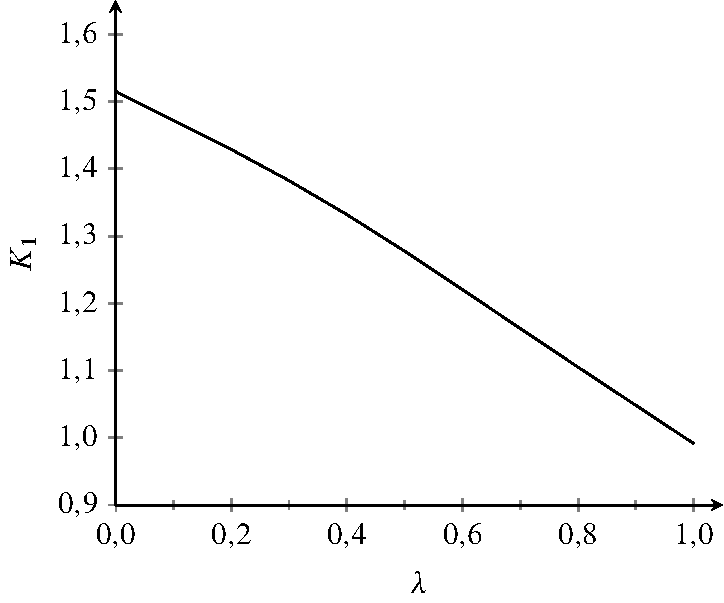
\includegraphics[width=0.65\textwidth]{images/plot_wing_ac_K1_vs_lambda.pdf}%
  \caption{\finalhyphendemerits=1000
           Coefficiente $K_1$ nella formula di calcolo del centro aerodinamico di un'ala finita.}
  \label{fig:Wing:Ac:K:One:Plots}%
\end%
    %{figure}%
    {SCfigure}%
%
%\EnlargedFigure% needs two latex passes
%    {t}% #1: t, b, p
%    {images/airfoil_geometry}% #2: the image file included by \includegraphics
%    {width=1.0\textwidth}% #3: option list to pass to \includegraphics, e.g. width=\linewidth,rotate=0
%    {\finalhyphendemerits=1000
%      Alcune caratteristiche geometriche di un profilo alare.}% #4: the caption text
%    {fig:Aero:Profilo:Geometria}% #5: the label
%\EnlargedFigureX% needs two latex passes
%  {t}% #1: t, b, p
%  {%
%    \makebox[\textwidth][c]{%
%    \includegraphics%
%      %[width=0.52\textwidth]%
%      % [height=5.5cm]%
%      [width=0.485\textwidth]%
%      {images/airfoil_Re_effect_polar.pdf}%
%    %\rule{8mm}{0pt}% <-- SPACER
%    \hfill
%    \raisebox{-0.6mm}[0pt][0pt]{%
%    \includegraphics%
%      %[width=0.52\textwidth]%
%      % [height=5.5cm]%
%      [width=0.485\textwidth]%
%      {images/airfoil_Re_effect_alpha_Cl.pdf}
%    }% end-of-raisebox
%    }% end-of-makebox
%  }% #2: the image file included by \includegraphics
%  {\finalhyphendemerits=1000
%    Influenza del numero di Reynolds, $\Reynolds_{\infty}=V_{\!\infty}c/\nu_{\infty}$,
%           sulla polare e sulla curva di portanza di un profilo NACA 64-212.%
%  }% #3: the caption text
%  {fig:Airfoil:Reynolds:Effects}%% #4: the label
%
%-----------------------------------------------------------------------------------------------

%-----------------------------------------------------------------------------------------------
%\begin%
%  %{figure}
%  {SCfigure}[1.9]%
%  [t]%[H]%[!htbp]
%  %\centering
%  %\checkoddpage
%  %\centering
%    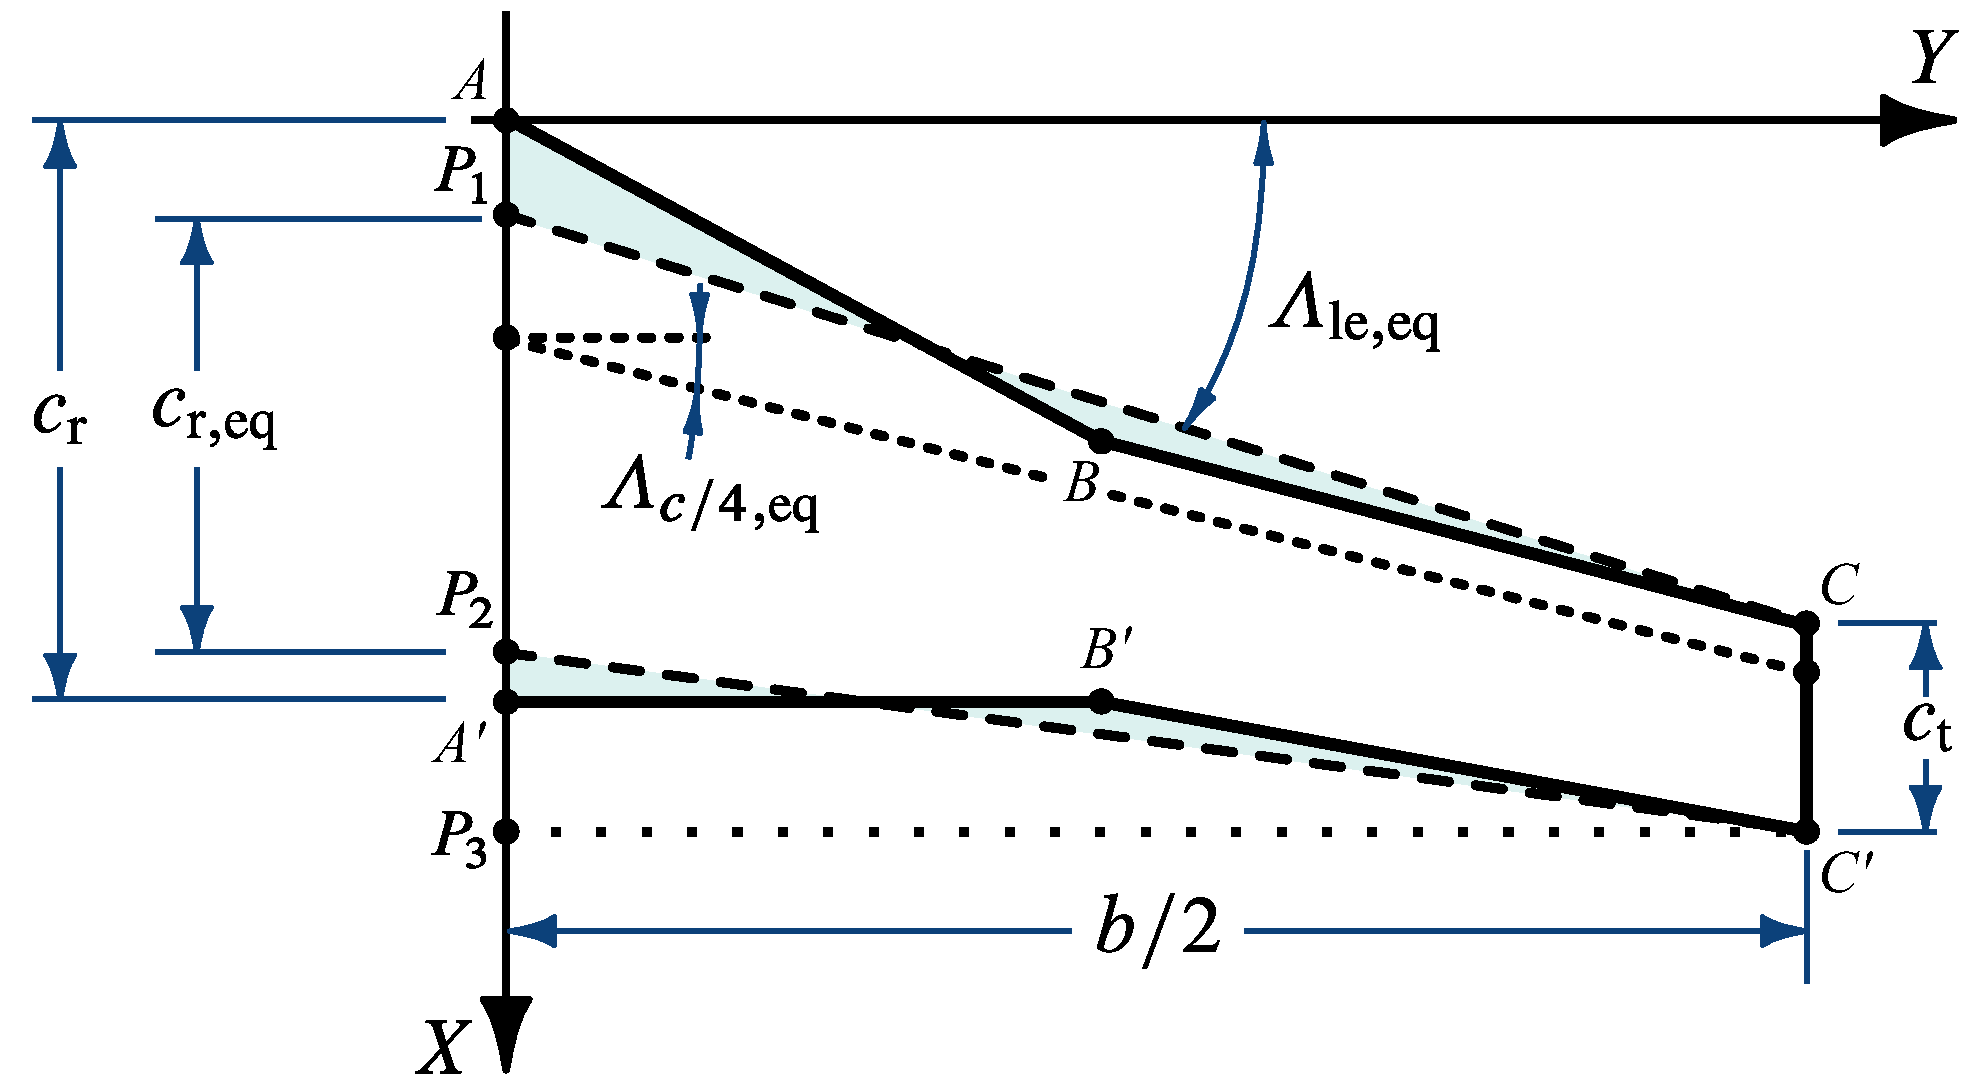
\includegraphics[width=0.78\textwidth]{images/equivalent_wing.pdf}%
%  \caption{\finalhyphendemerits=1000
%           Ala a bordi d'attacco e d'uscita non rettilinei ed ala equivalente a bordi dritti.}
%  \label{fig:Equivalent:Wing:Planform:Defs}%
%\end%
%    %{figure}%
%    {SCfigure}%
%
%\EnlargedFigure% needs two latex passes
%    {t}% #1: t, b, p
%    {images/airfoil_geometry}% #2: the image file included by \includegraphics
%    {width=1.0\textwidth}% #3: option list to pass to \includegraphics, e.g. width=\linewidth,rotate=0
%    {\finalhyphendemerits=1000
%      Alcune caratteristiche geometriche di un profilo alare.}% #4: the caption text
%    {fig:Aero:Profilo:Geometria}% #5: the label
\EnlargedFigureX% needs two latex passes
  {p}% #1: t, b, p
  {%
    \centering
    \begin{tabular}{@{}c@{\rule{3mm}{0pt}}c@{}}
      \includegraphics%
        %[width=0.52\textwidth]%
        % [height=5.5cm]%
        [width=0.485\textwidth]%
        {images/plot_wing_ac_K2_lam0.pdf}
      &
      \includegraphics%
        %[width=0.52\textwidth]%
        % [height=5.5cm]%
        [width=0.485\textwidth]%
        {images/plot_wing_ac_K2_lam02.pdf}
      \\
      \includegraphics%
        %[width=0.52\textwidth]%
        % [height=5.5cm]%
        [width=0.485\textwidth]%
        {images/plot_wing_ac_K2_lam04.pdf}
      &
      \includegraphics%
        %[width=0.52\textwidth]%
        % [height=5.5cm]%
        [width=0.485\textwidth]%
        {images/plot_wing_ac_K2_lam06.pdf}
      \\
      \includegraphics%
        %[width=0.52\textwidth]%
        % [height=5.5cm]%
        [width=0.485\textwidth]%
        {images/plot_wing_ac_K2_lam08.pdf}
      &
      \includegraphics%
        %[width=0.52\textwidth]%
        % [height=5.5cm]%
        [width=0.485\textwidth]%
        {images/plot_wing_ac_K2_lam1.pdf}
    \end{tabular}
  }% #2: the image file included by \includegraphics
  {\finalhyphendemerits=1000
    Coefficiente $K_2$ nella formula di calcolo del centro aerodinamico di un'ala finita.%
  }% #3: the caption text
  {fig:Wing:Ac:K:Two:Plots}%% #4: the label
%
%-----------------------------------------------------------------------------------------------

%-----------------------------------------------------------------------------------------------
%\begin%
%  %{figure}
%  {SCfigure}[1.9]%
%  [t]%[H]%[!htbp]
%  %\centering
%  %\checkoddpage
%  %\centering
%    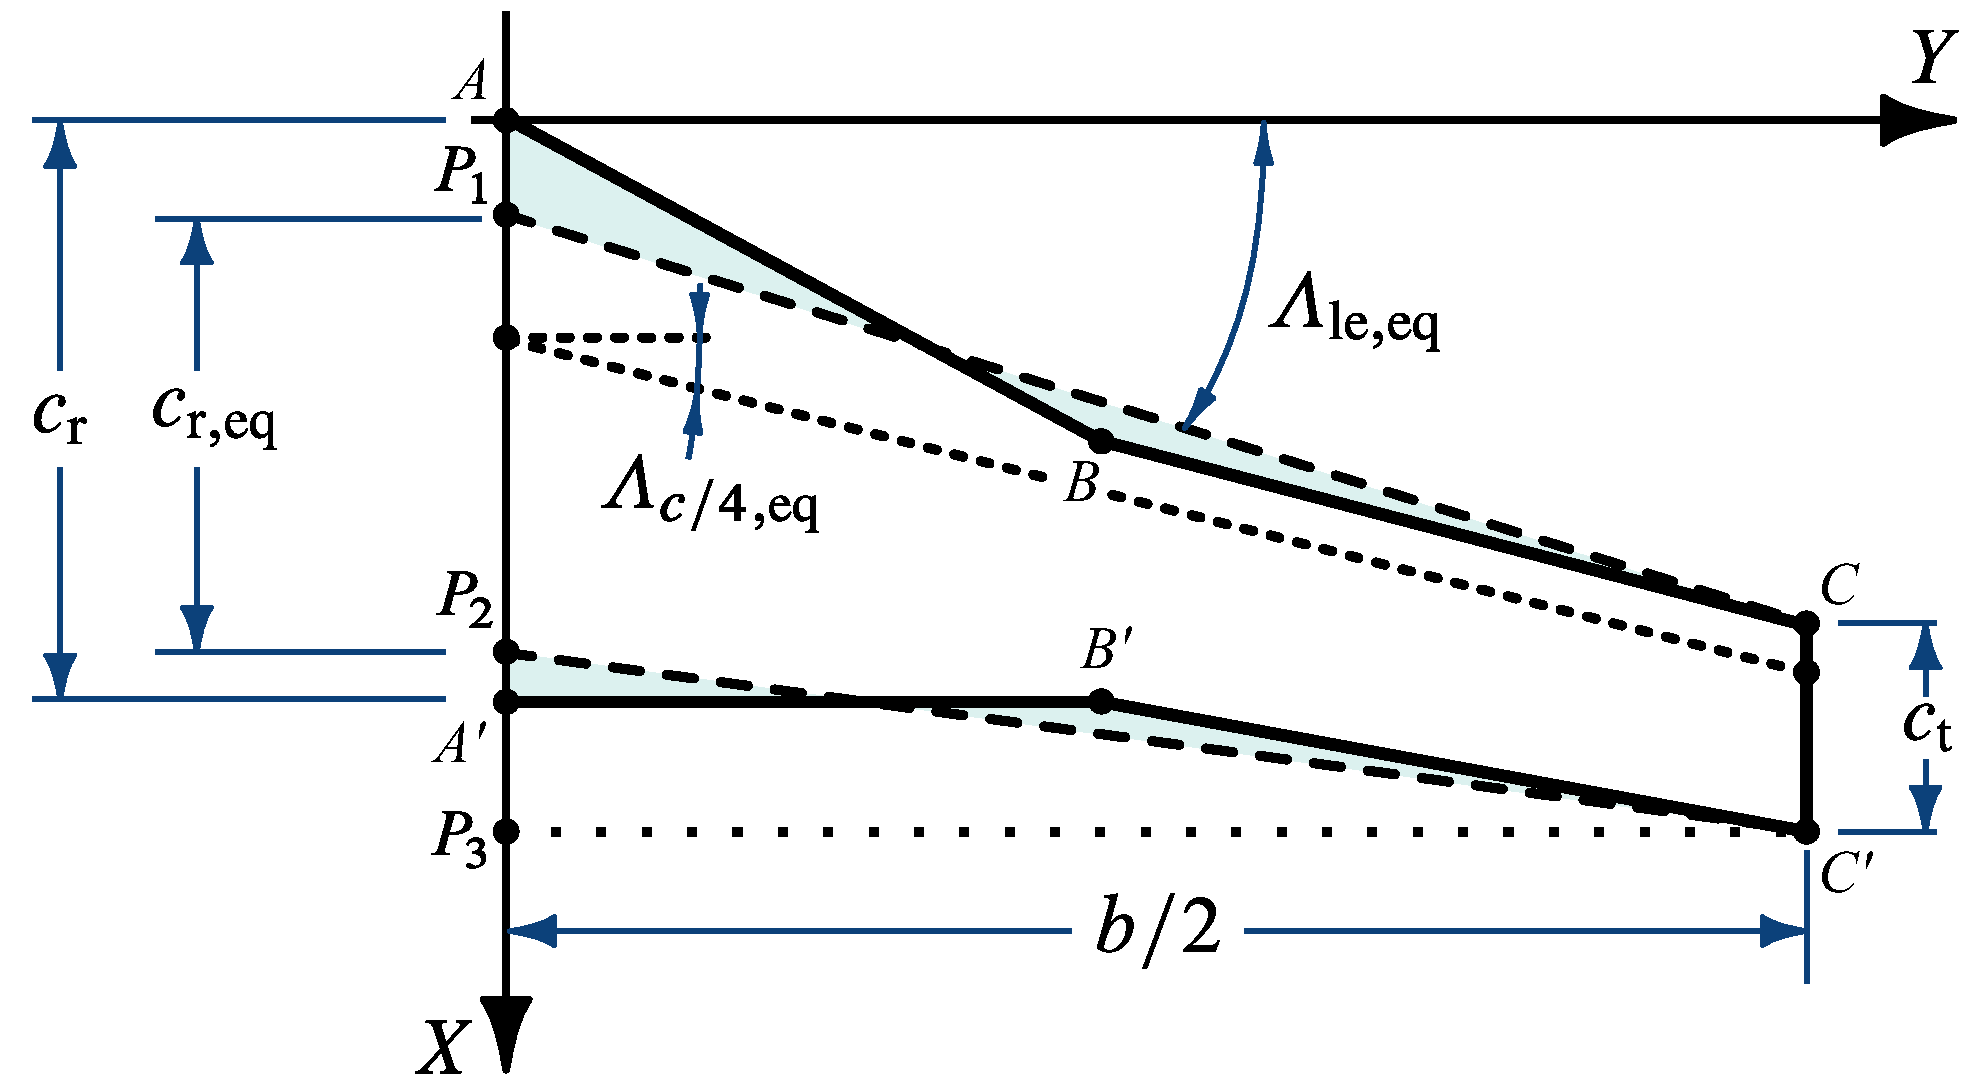
\includegraphics[width=0.78\textwidth]{images/equivalent_wing.pdf}%
%  \caption{\finalhyphendemerits=1000
%           Ala a bordi d'attacco e d'uscita non rettilinei ed ala equivalente a bordi dritti.}
%  \label{fig:Equivalent:Wing:Planform:Defs}%
%\end%
%    %{figure}%
%    {SCfigure}%
%
%\EnlargedFigure% needs two latex passes
%    {t}% #1: t, b, p
%    {images/airfoil_geometry}% #2: the image file included by \includegraphics
%    {width=1.0\textwidth}% #3: option list to pass to \includegraphics, e.g. width=\linewidth,rotate=0
%    {\finalhyphendemerits=1000
%      Alcune caratteristiche geometriche di un profilo alare.}% #4: the caption text
%    {fig:Aero:Profilo:Geometria}% #5: the label
\EnlargedFigureX% needs two latex passes
  {p}% #1: t, b, p
  {%
    \centering
    \begin{tabular}{@{}c@{\rule{3mm}{0pt}}c@{}}
      \includegraphics%
        %[width=0.52\textwidth]%
        % [height=5.5cm]%
        [width=0.485\textwidth]%
        {images/plot_xbar_prime_wing_ac_lam0.pdf}
      &
      \includegraphics%
        %[width=0.52\textwidth]%
        % [height=5.5cm]%
        [width=0.485\textwidth]%
        {images/plot_xbar_prime_wing_ac_lam02.pdf}
      \\
      \includegraphics%
        %[width=0.52\textwidth]%
        % [height=5.5cm]%
        [width=0.485\textwidth]%
        {images/plot_xbar_prime_wing_ac_lam025.pdf}
      &
      \includegraphics%
        %[width=0.52\textwidth]%
        % [height=5.5cm]%
        [width=0.485\textwidth]%
        {images/plot_xbar_prime_wing_ac_lam033.pdf}
      \\
      \includegraphics%
        %[width=0.52\textwidth]%
        % [height=5.5cm]%
        [width=0.485\textwidth]%
        {images/plot_xbar_prime_wing_ac_lam05.pdf}
      &
      \includegraphics%
        %[width=0.52\textwidth]%
        % [height=5.5cm]%
        [width=0.485\textwidth]%
        {images/plot_xbar_prime_wing_ac_lam1.pdf}
    \end{tabular}
  }% #2: the image file included by \includegraphics
  {\finalhyphendemerits=1000
    Posizione adimensionale $X'_\text{ac}/c_\text{r}$ nella formula di calcolo del centro aerodinamico 
    di un'ala finita.%
  }% #3: the caption text
  {fig:Wing:Ac:X:AC:From:Apex:Plots}%% #4: the label
%
%-----------------------------------------------------------------------------------------------

%=BEGING-ES===========================================================================================
%
\def\mySpanWingMT{10.600000}
\def\mySpanWingIMT{6.360000}
\def\mySpanWingIIMT{4.240000}
\def\myChordRootWingMT{1.440000}
\def\myChordRootWingIMT{1.440000}
\def\myChordRootWingIIMT{1.440000}
\def\myChordTipWingMT{0.860000}
\def\myChordTipWingIMT{1.440000}
\def\myChordTipWingIIMT{0.860000}
\def\mySweepLEWingIIDEG{0.000000}
\def\myCoeffAChordWingI{0.000000}
\def\myCoeffBChordWingIMT{1.440000}
\def\myCoeffAChordWingII{-0.273585}
\def\myCoeffBChordWingIIMT{1.440000}
\def\myAlphaZeroLiftRootWingIDEG{-2.500000}
\def\myAlphaZeroLiftTipWingIDEG{-2.500000}
\def\myAlphaZeroLiftRootWingIRAD{-0.043633}
\def\myAlphaZeroLiftTipWingIRAD{-0.043633}
\def\myAlphaZeroLiftRootWingIIDEG{-2.500000}
\def\myAlphaZeroLiftTipWingIIDEG{-1.000000}
\def\myAlphaZeroLiftRootWingIIRAD{-0.043633}
\def\myAlphaZeroLiftTipWingIIRAD{-0.017453}
\def\myTaperRatioWingI{1.000000}
\def\myTaperRatioWingII{0.597222}
\def\myTwistWingIDEG{0.000000}
\def\myTwistWingIRAD{0.000000}
\def\myTwistWingIIDEG{-3.000000}
\def\myTwistWingIIRAD{-0.052360}
\def\myAreaWingIMTsquared{9.158400}
\def\myAreaWingIIMTsquared{4.876000}
\def\myAreaWingMTsquared{14.034400}
\def\myCoeffAAeroTwistWingIRADMT{0.000000}
\def\myCoeffBAeroTwistWingIRAD{-0.043633}
\def\myCoeffAAeroTwistWingIIRADMT{0.012349}
\def\myCoeffBAeroTwistWingIIRAD{-0.043633}
\def\myCoeffATwistWingIRADMT{0.000000}
\def\myCoeffATwistWingIIRADMT{-0.024698}
\def\myCoeffBTwistWingIRAD{0.000000}
\def\myCoeffBTwistWingIIRAD{0.000000}
\def\myAlphaZeroLiftWingIRAD{-0.028653}
\def\myAlphaZeroLiftWingIDEG{-1.641680}
\def\myAlphaZeroLiftWingIIRAD{0.008329}
\def\myAlphaZeroLiftWingIIDEG{0.477233}
\def\myAlphaZeroLiftWingRAD{-0.020323}
\def\myAlphaZeroLiftWingDEG{-1.164447}

%
\begin{myExampleX}{Centro aerodinamico di un'ala cranked}{\ding{46}\ \myIconGraph\ }% \ \Keyboard\ %
\label{example:Wing:Aerodynamic:Center:Cranked}
%
\noindent
In questo esempio verrà calcolata la posizione del centro aerodinamico
di un'ala simile a quella di un Boeing~787.
L'ala considerata è di tipo \emph{cranked}, come si vede dalla forma in pianta riportata nella
figura~\ref{fig:Wing:Aerodynamic:Center:Cranked:Panels}, e possiede le seguenti caratteristiche:

\smallskip
\noindent
\adjustbox{center=\textwidth}{%
 \underline{\emph{Pannello 1} (pannello interno)}
}

\smallskip
\noindent
\adjustbox{left=\textwidth}{%
  \adjustbox{right=0.39\textwidth}{%
    \emph{corde}:
  }\rule{0.5em}{0pt}% --> SPACER
  \adjustbox{left=0.59\textwidth}{%
    $c_{\mathrm{r},1}=\SI[round-precision=2]{\myChordRootWingIMT}{\metre}$,
    $c_{\mathrm{t},1}=\SI[round-precision=2]{\myChordTipWingIMT}{\metre}$,
    $\lambda_1 = \SI[round-precision=2]{\myTaperRatioWingI}{}$,
  }%
}

\smallskip
\noindent
\adjustbox{left=\textwidth}{%
  \adjustbox{right=0.39\textwidth}{%
    \emph{apertura e superficie}:
  }\rule{0.5em}{0pt}% --> SPACER
  \adjustbox{left=0.59\textwidth}{%
    $b_1=\SI[round-precision=2]{\mySpanWingIMT}{\metre}$,
    $S_1=\SI[round-precision=2]{\myAreaWingIMTsquared}{\meter^2}$,
    $\AR_1 = \SI[round-precision=2]{\myAspectRatioWingI}{}$,
  }%
}

\smallskip
\noindent
\adjustbox{left=\textwidth}{%
  \adjustbox{right=0.39\textwidth}{%
    \emph{angoli di freccia}:
  }\rule{0.5em}{0pt}% --> SPACER
  \adjustbox{left=0.59\textwidth,minipage=[t]{0.59\textwidth}}{%
    $\Lambda_\mathrm{le,1}=\SI[round-precision=4]{\mySweepLEWingIRAD}{\radian}=\SI[round-precision=1]{\mySweepLEWingIDEG}{\deg}$,
    \\
    $\Lambda_\mathrm{te,1}=\SI[round-precision=4]{\mySweepTEWingIRAD}{\radian}=\SI[round-precision=1]{\mySweepTEWingIDEG}{\deg}$,
  }%
}

\smallskip
\noindent
\adjustbox{left=\textwidth}{%
  \adjustbox{right=0.39\textwidth}{%
    \emph{gradienti $C_{\ell_\mathlarger{\alpha}}$ di profilo}:
  }\rule{0.5em}{0pt}% --> SPACER
  \adjustbox{left=0.59\textwidth,minipage=[t]{0.59\textwidth}}{%
    $C_{\ell_\mathlarger{\alpha},\mathrm{r},1}=\SI[round-precision=2]{\myCLAlphaRootWingIRAD}{\radian^{-1}}=\SI[round-precision=4]{\myCLAlphaRootWingIDEG}{\deg^{-1}}$,
    \\
    $C_{\ell_\mathlarger{\alpha},\mathrm{t},1}=\SI[round-precision=2]{\myCLAlphaTipWingIRAD}{\radian^{-1}}=\SI[round-precision=4]{\myCLAlphaTipWingIDEG}{\deg^{-1}}$,
  }%
}

\smallskip
\noindent
\adjustbox{left=\textwidth}{%
  \adjustbox{right=0.39\textwidth}{%
    \emph{svergolamenti}:
  }\rule{0.5em}{0pt}% --> SPACER
  \adjustbox{left=0.59\textwidth,minipage=[t]{0.59\textwidth}}{%
    $\alpha_{0\ell,\mathrm{r},1}=\SI[round-precision=3]{\myAlphaZeroLiftRootWingIRAD}{\radian}
      =\SI[round-precision=1]{\myAlphaZeroLiftRootWingIDEG}{\deg}$,\\
    $\alpha_{0\ell,\mathrm{t},1}=\SI[round-precision=3]{\myAlphaZeroLiftTipWingIRAD}{\radian}
      =\SI[round-precision=1]{\myAlphaZeroLiftTipWingIDEG}{\deg}$,\\
    $\epsilon_{\mathrm{g,t},1}=\SI[round-precision=3]{\myTwistWingIRAD}{\radian}
      =\SI[round-precision=1]{\myTwistWingIDEG}{\deg}$,
  }%
}

\smallskip
\noindent
\adjustbox{left=\textwidth}{%
  \adjustbox{right=0.39\textwidth}{%
    \emph{centri aerodinamici di profilo}:
  }\rule{0.5em}{0pt}% --> SPACER
  \adjustbox{left=0.59\textwidth}{%
    $\bar{x}_{\mathrm{ac,2D,1},\mathrm{r}}=\SI[round-precision=2]{\myXsiacRootWingI}{}$,
    $\bar{x}_{\mathrm{ac,2D,1},\mathrm{t}}=\SI[round-precision=2]{\myXsiacTipWingI}{}$,
  }%
}

\smallskip
\noindent
\adjustbox{left=\textwidth}{%
  \adjustbox{right=0.39\textwidth}{%
    \emph{coefficienti $C_{\mathcal{m}_\mathlarger{\mathrm{ac}}}$ di profilo}:
  }\rule{0.5em}{0pt}% --> SPACER
  \adjustbox{left=0.59\textwidth}{%
    $C_{\mathcal{m}_\mathlarger{\mathrm{ac}},\mathrm{r},1}=\SI[round-precision=3]{\myCmZeroRootWingI}{}$,
    $C_{\mathcal{m}_\mathlarger{\mathrm{ac}},\mathrm{t},1}=\SI[round-precision=3]{\myCmZeroTipWingI}{}$,
  }%
}

\medskip
\noindent
\adjustbox{center=\textwidth}{%
 \underline{\emph{Pannello 2} (pannello esterno)}
}

\smallskip
\noindent
\adjustbox{left=\textwidth}{%
  \adjustbox{right=0.39\textwidth}{%
    \emph{corde}:
  }\rule{0.5em}{0pt}% --> SPACER
  \adjustbox{left=0.59\textwidth}{%
    $c_{\mathrm{r},2}=\SI[round-precision=2]{\myChordRootWingIIMT}{\metre}$,
    $c_{\mathrm{t},2}=\SI[round-precision=2]{\myChordTipWingIIMT}{\metre}$,
    $\lambda_2 = \SI[round-precision=2]{\myTaperRatioWingII}{}$,
  }%
}

\smallskip
\noindent
\adjustbox{left=\textwidth}{%
  \adjustbox{right=0.39\textwidth}{%
    \emph{apertura e superficie}:
  }\rule{0.5em}{0pt}% --> SPACER
  \adjustbox{left=0.59\textwidth}{%
    $b_2=\SI[round-precision=2]{\mySpanWingIIMT}{\metre}$,
    $S_2=\SI[round-precision=2]{\myAreaWingIIMTsquared}{\meter^2}$,
    $\AR_2 = \SI[round-precision=2]{\myAspectRatioWingII}{}$,
  }%
}

\smallskip
\noindent
\adjustbox{left=\textwidth}{%
  \adjustbox{right=0.39\textwidth}{%
    \emph{angoli di freccia}:
  }\rule{0.5em}{0pt}% --> SPACER
  \adjustbox{left=0.59\textwidth,minipage=[t]{0.59\textwidth}}{%
    $\Lambda_\mathrm{le,2}=\SI[round-precision=4]{\mySweepLEWingIIRAD}{\radian}=\SI[round-precision=1]{\mySweepLEWingIIDEG}{\deg}$,
    \\
    $\Lambda_\mathrm{te,2}=\SI[round-precision=4]{\mySweepTEWingIIRAD}{\radian}=\SI[round-precision=1]{\mySweepTEWingIIDEG}{\deg}$,
  }%
}

\smallskip
\noindent
\adjustbox{left=\textwidth}{%
  \adjustbox{right=0.39\textwidth}{%
    \emph{gradienti $C_{\ell_\mathlarger{\alpha}}$ di profilo}:
  }\rule{0.5em}{0pt}% --> SPACER
  \adjustbox{left=0.59\textwidth,minipage=[t]{0.59\textwidth}}{%
    $C_{\ell_\mathlarger{\alpha},\mathrm{r},2}=\SI[round-precision=2]{\myCLAlphaRootWingIIRAD}{\radian^{-1}}=\SI[round-precision=4]{\myCLAlphaRootWingIIDEG}{\deg^{-1}}$,
    \\
    $C_{\ell_\mathlarger{\alpha},\mathrm{t},2}=\SI[round-precision=2]{\myCLAlphaTipWingIIRAD}{\radian^{-1}}=\SI[round-precision=4]{\myCLAlphaTipWingIIDEG}{\deg^{-1}}$,
  }%
}

\smallskip
\noindent
\adjustbox{left=\textwidth}{%
  \adjustbox{right=0.39\textwidth}{%
    \emph{svergolamenti}:
  }\rule{0.5em}{0pt}% --> SPACER
  \adjustbox{left=0.59\textwidth,minipage=[t]{0.59\textwidth}}{%
    $\alpha_{0\ell,\mathrm{r},2}=\SI[round-precision=3]{\myAlphaZeroLiftRootWingIIRAD}{\radian}
      =\SI[round-precision=1]{\myAlphaZeroLiftRootWingIIDEG}{\deg}$,\\
    $\alpha_{0\ell,\mathrm{t},2}=\SI[round-precision=3]{\myAlphaZeroLiftTipWingIIRAD}{\radian}
      =\SI[round-precision=1]{\myAlphaZeroLiftTipWingIIDEG}{\deg}$,\\
    $\epsilon_{\mathrm{g,t},2}=\SI[round-precision=3]{\myTwistWingIIRAD}{\radian}
      =\SI[round-precision=1]{\myTwistWingIIDEG}{\deg}$,
  }%
}

\smallskip
\noindent
\adjustbox{left=\textwidth}{%
  \adjustbox{right=0.39\textwidth}{%
    \emph{centri aerodinamici di profilo}:
  }\rule{0.5em}{0pt}% --> SPACER
  \adjustbox{left=0.59\textwidth}{%
    $\bar{x}_{\mathrm{ac,2D,2},\mathrm{r}}=\SI[round-precision=2]{\myXsiacRootWingII}{}$,
    $\bar{x}_{\mathrm{ac,2D,2},\mathrm{t}}=\SI[round-precision=2]{\myXsiacTipWingII}{}$,
  }%
}

\smallskip
\noindent
\adjustbox{left=\textwidth}{%
  \adjustbox{right=0.39\textwidth}{%
    \emph{coefficienti $C_{\mathcal{m}_\mathlarger{\mathrm{ac}}}$ di profilo}:
  }\rule{0.5em}{0pt}% --> SPACER
  \adjustbox{left=0.59\textwidth}{%
    $C_{\mathcal{m}_\mathlarger{\mathrm{ac}},\mathrm{r},2}=\SI[round-precision=3]{\myCmZeroRootWingII}{}$,
    $C_{\mathcal{m}_\mathlarger{\mathrm{ac}},\mathrm{t},2}=\SI[round-precision=3]{\myCmZeroTipWingII}{}$,
  }%
}

\medskip
\noindent
\adjustbox{left=\textwidth}{%
  \adjustbox{right=0.39\textwidth}{%
    \emph{condizione di volo}:
  }\rule{0.5em}{0pt}% --> SPACER
  \adjustbox{left=0.59\textwidth}{%
    $\Mach = \SI[round-precision=2]{\myMach}{}$.
  }%
}

%-----------------------------------------------------------------------------------------------
\begin%
  %{figure}
  {SCfigure}[1.9]%
  [t]%[H]%[!htbp]
  %\centering
  %\checkoddpage
  %\centering
    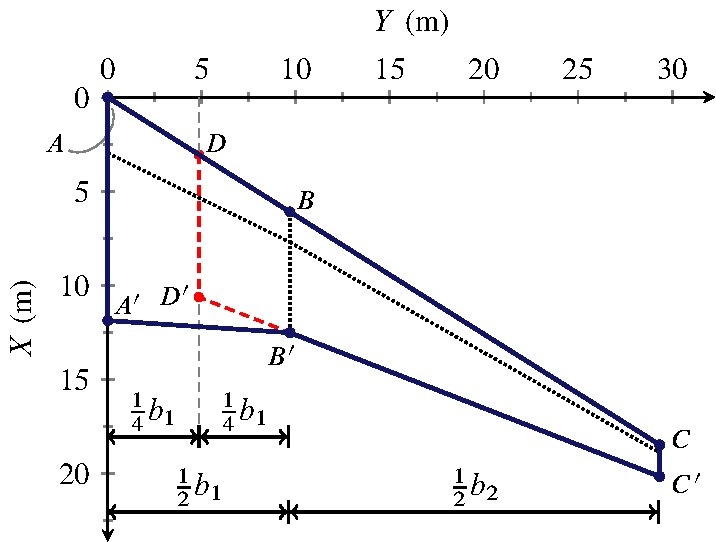
\includegraphics[width=0.72\textwidth]{exercises/wing_ac_cranked_1/wing_ac_cranked_1_drawing_panels.pdf}%
  \caption{\finalhyphendemerits=1000
           Ala \emph{cranked} proposta nell'esempio~\ref{example:Wing:Aerodynamic:Center:Cranked}.
           Sono evidenziati il pannello interno $ABB'A'$, il pannello esterno $BCC'B'$ e il pannello esterno esteso $DCC'D'$ 
           (\emph{constructed panel}) utilizzato per il calcolo del centro aerodinamico dell'ala.
  }
  \label{fig:Wing:Aerodynamic:Center:Cranked:Panels}%
\end%
    %{figure}%
    {SCfigure}%
%
%\EnlargedFigure% needs two latex passes
%    {t}% #1: t, b, p
%    {images/airfoil_geometry}% #2: the image file included by \includegraphics
%    {width=1.0\textwidth}% #3: option list to pass to \includegraphics, e.g. width=\linewidth,rotate=0
%    {\finalhyphendemerits=1000
%      Alcune caratteristiche geometriche di un profilo alare.}% #4: the caption text
%    {fig:Aero:Profilo:Geometria}% #5: the label
%\EnlargedFigureX% needs two latex passes
%  {t}% #1: t, b, p
%  {%
%    \begin{tabular}{@{}c@{}}
%    \makebox[\textwidth][c]{%
%      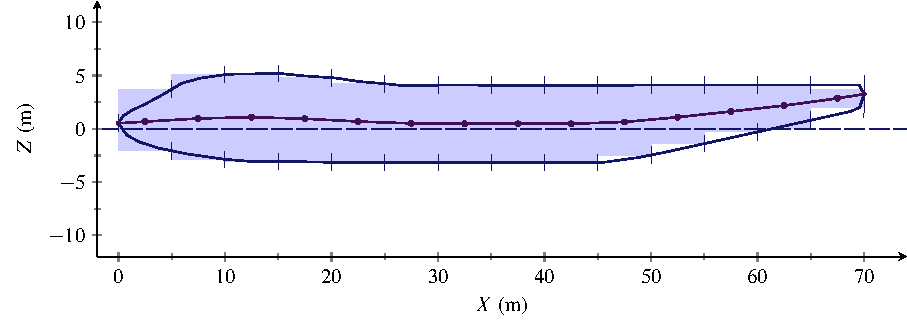
\includegraphics[width=1.00\textwidth]{exercises/fuselage_multhopp_1/fuselage_sideview_1.pdf}%
%    }% end-of-makebox
%    \\
%    \makebox[\textwidth][c]{%
%      \rule{2.2mm}{0pt}% --> hack
%      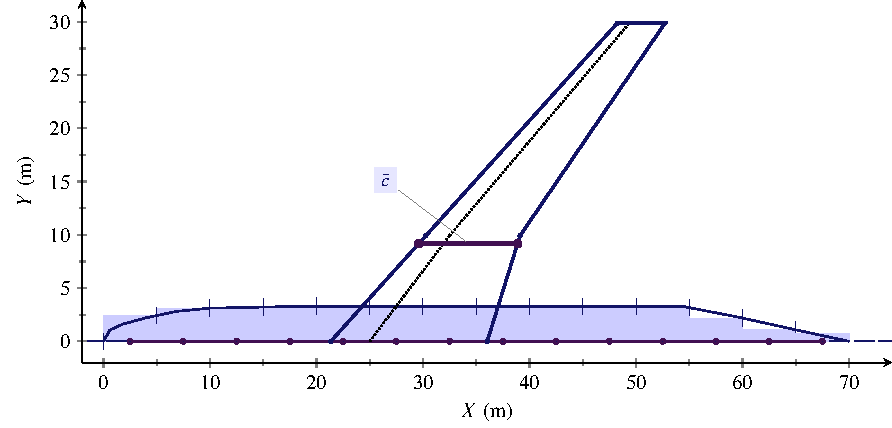
\includegraphics[width=0.98\textwidth]{exercises/fuselage_multhopp_1/fuselage_topview_1.pdf}%
%    }% end-of-makebox
%    \end{tabular}
%    \vspace{0.3cm}
%  }% #2: the image file included by \includegraphics
%  {\finalhyphendemerits=1000
%    Fusoliera assegnata nell'esempio~\ref{example:Fuselage:Multhopp:A}.
%    Discretizzazione della proiezione laterale per il calcolo approssimato dei coefficienti
%    \smash{$C_{\mathcal{M}0,\Body}$} e \smash{$C_{\mathcal{M}_\mathlarger{\alpha},\Body}$}
%    con il metodo di integrazione per strisce di Multhopp.
%  }% #3: the caption text
%  {fig:Fuselage:Multhopp:Results:AA}%% #4: the label
%
%-----------------------------------------------------------------------------------------------

\bigskip

Dai dati si ricava agevolmente la legge delle corde
\[
c(Y)=
\ccases{
%\left\{
%\begin{array}{cl}
c_1(Y) = A_{c,1} \, Y + B_{c,1} & \text{per }\makebox[3em][r]{$0$}     \le Y \le \frac{1}{2}b_1
\\[4pt]
c_2(Y) = A_{c,2} \, \bigg(Y-\dfrac{b_1}{2}\bigg) + B_{c,2} & \text{per }\makebox[3em][r]{$\frac{1}{2}b_1$}< Y \le \frac{1}{2}b
%\end{array}
%\right.
}
\]
con
\[
A_{c,1}
  = \frac{c_{\mathrm{t},1} - c_{\mathrm{r},1}}{b_1/2}
  = 
    2 \frac{
      \SI[round-precision=2]{\myChordTipWingIMT}{\metre} - \SI[round-precision=2]{\myChordRootWingIMT}{\metre}
    }{
      \SI[round-precision=2]{\mySpanWingIMT}{\metre}
    }
  = \mathunderline{mydarkblue}{ \SI[round-precision=3]{\myCoeffAChordWingI}{} }
\]
\[
B_{c,1}
  = c_{\mathrm{r},1}
  = \mathunderline{mydarkblue}{ \SI[round-precision=2]{\myCoeffBChordWingIMT}{\metre} }
\]
\[
A_{c,2}
  = \frac{c_{\mathrm{t},2} - c_{\mathrm{r},2}}{b_2/2}
  = 
    2 \frac{
      \SI[round-precision=2]{\myChordTipWingIIMT}{\metre} - \SI[round-precision=2]{\myChordRootWingIIMT}{\metre}
    }{
      \SI[round-precision=2]{\mySpanWingIIMT}{\metre}
    }
  = \mathunderline{mydarkblue}{ \SI[round-precision=3]{\myCoeffAChordWingII}{} }
\]
\[
B_{c,2}
  = c_{\mathrm{r},2}
  = \mathunderline{mydarkblue}{ \SI[round-precision=2]{\myCoeffBChordWingIIMT}{\metre} }
\]
Pertanto, risulta
\[
c(Y)=
\ccases{
%\left\{
%\begin{array}{cl}
c_1(Y) = 
  \SI[round-precision=3]{\myCoeffAChordWingI}{} \, Y 
    + \SI[round-precision=2]{\myCoeffBChordWingIIMT}{\metre} 
  & \text{per }
    \makebox[3.5em][r]{$\SI[round-precision=0]{0}{\metre}$} 
      \le Y \le 
      \calcSI[round-precision=2,fixed-exponent=0,scientific-notation=fixed]{0.5*\mySpanWingIMT}{\metre}
\\[4pt]
c_2(Y) 
  = \SI[round-precision=3]{\myCoeffAChordWingII}{} \, 
    \big(
      Y
      - \calcSI[round-precision=2,fixed-exponent=0,scientific-notation=fixed]{0.5*\mySpanWingIMT}{\metre}
    \big)
    + \SI[round-precision=2]{\myCoeffBChordWingIIMT}{\metre} 
  & \text{per }
    \makebox[3.5em][r]{%
      $\calcSI[round-precision=2,fixed-exponent=0,scientific-notation=fixed]{0.5*\mySpanWingIMT}{\metre}$
    }% end-of-makebox
      < Y 
      \le \calcSI[round-precision=2,fixed-exponent=0,scientific-notation=fixed]{0.5*\mySpanWingMT}{\metre}
%\end{array}
%\right.
}
\]

Dalla figura~\ref{fig:Wing:Aerodynamic:Center:Cranked:Panels} si osservano
i punti $A$, $B$, $B'$ e $A'$ che definiscono la porzione interna dell'ala.
Il pannello interno ha un rapporto di rastremazione
\[
\lambda_1
  =\frac{c_{\mathrm{t},1}}{c_{\mathrm{r},1}}
  =\frac{\SI[round-precision=2]{\myChordTipWingIMT}{\metre}}{\SI[round-precision=2]{\myChordRootWingIMT}{\metre}}
  =\mathunderline{mydarkblue}{ \SI[round-precision=2]{\myTaperRatioWingI}{} }
\]
una superficie
\[
S_1 = \frac{b_1}{2} \, c_{\mathrm{r},1} \, \big( 1 + \lambda_1 \big)
  =
    \num{0.5} \cdot \SI[round-precision=1]{\mySpanWingIMT}{\metre}
      \cdot \SI[round-precision=2]{\myChordRootWingIMT}{\metre}
      \cdot \big( 1 + \SI[round-precision=2]{\myTaperRatioWingI}{} \big) 
    = \mathunderline{mydarkblue}{ \SI[round-precision=1]{\myAreaWingIMTsquared}{\metre^2} }
\]
e un allungamento
\[
\AR_1 
  = \frac{b_1^2}{S_1}
  = \frac{\big(\SI[round-precision=1]{\mySpanWingIMT}{\metre}\big)^2}{\SI[round-precision=1]{\myAreaWingIMTsquared}{\metre^2}}
  = \mathunderline{mydarkblue}{ \num[round-precision=2]{\myAspectRatioWingI} }
\]
Da tali valori si ricava una corda media aerodinamica
\[
\begin{split}
\bar{c}_1 & {}= \frac{2}{3} \, c_{\mathrm{r},1} \, \frac{1+\lambda_1 + \lambda_1^2}{1+\lambda_1} \\
  & {}=
    \num{0.667} \cdot \SI[round-precision=2]{\myChordRootWingIMT}{\metre}
      \cdot 
        \frac{
          1 + \SI[round-precision=2]{\myTaperRatioWingI}{} + \SI[round-precision=2]{\myTaperRatioWingI}{}^2
        }{
          1 + \SI[round-precision=2]{\myTaperRatioWingI}{}
        }
    = \mathunderline{mydarkblue}{ \SI[round-precision=2]{\myMACWingIMT}{\metre} }
\end{split}
\]
La sezione alare del pannello interno avente corda $\bar{c}_1$ ha bordo d'attacco
di ascissa
\[
\begin{split}
X_{\mathrm{le},\bar{c}_1} 
  & {}=
    \frac{b_1}{6} \, \frac{1+2\lambda_1}{1+\lambda_1} \tan\Lambda_\mathrm{le,1} \\[3pt]
  & {}=
    \frac{\SI[round-precision=1]{\mySpanWingIMT}{\metre}}{6}
      \cdot 
      \frac{
        1 + 2\cdot\SI[round-precision=2]{\myTaperRatioWingI}{}
      }{
        1 + \SI[round-precision=2]{\myTaperRatioWingI}{}
      }
      \cdot \tan \big( \SI[round-precision=3]{\mySweepLEWingIRAD}{\radian} \big)
    = \mathunderline{mydarkblue}{ \SI[round-precision=2]{\myXMACLEToApexWingIMT}{\metre} }
\end{split}
\]
corrispondente alla stazione
\[
\begin{split}
Y_{\bar{c}_1} 
  & {}=
    \frac{b_1}{6} \, \frac{1+2\lambda_1}{1+\lambda_1} \\[3pt]
  & {}=
    \frac{\SI[round-precision=1]{\mySpanWingIMT}{\metre}}{6}
      \cdot 
      \frac{
        1 + 2\cdot\SI[round-precision=2]{\myTaperRatioWingI}{}
      }{
        1 + \SI[round-precision=2]{\myTaperRatioWingI}{}
      }
    = \mathunderline{mydarkblue}{ \SI[round-precision=2]{\myYMACWingIMT}{\metre} }
\end{split}
\]
lungo l'apertura alare.

Analogamente, dalla figura~\ref{fig:Wing:Aerodynamic:Center:Cranked:Panels} si osservano
i punti $B$, $C$, $C'$ e $B'$ che definiscono la porzione esterna dell'ala.
Per il pannello esterno si ha un rapporto di rastremazione
\[
\lambda_2
  =\frac{c_{\mathrm{t},2}}{c_{\mathrm{r},2}}
  =\frac{\SI[round-precision=2]{\myChordTipWingIIMT}{\metre}}{\SI[round-precision=2]{\myChordRootWingIIMT}{\metre}}
  =\mathunderline{mydarkblue}{ \SI[round-precision=2]{\myTaperRatioWingII}{} }
\]
una superficie
\[
S_2 = \frac{b_2}{2} \, c_{\mathrm{r},2} \, \big( 1 + \lambda_2 \big)
  =
    \num{0.5} \cdot \SI[round-precision=1]{\mySpanWingIIMT}{\metre}
      \cdot \SI[round-precision=2]{\myChordRootWingIIMT}{\metre}
      \cdot \big( 1 + \SI[round-precision=2]{\myTaperRatioWingII}{} \big) 
    = \mathunderline{mydarkblue}{ \SI[round-precision=1]{\myAreaWingIIMTsquared}{\metre^2} }
\]
e un allungamento
\[
\AR_2 
  = \frac{b_2^2}{S_2}
  = \frac{\big(\SI[round-precision=1]{\mySpanWingIIMT}{\metre}\big)^2}{\SI[round-precision=1]{\myAreaWingIIMTsquared}{\metre^2}}
  = \mathunderline{mydarkblue}{ \num[round-precision=2]{\myAspectRatioWingII} }
\]

Conseguentemente, si ha una corda media aerodinamica
\[
\begin{split}
\bar{c}_2 & {}= \frac{2}{3} \, c_{\mathrm{r},2} \, \frac{1+\lambda_2 + \lambda_2^2}{1+\lambda_2} \\
  & {}=
    \num{0.667} \cdot \SI[round-precision=2]{\myChordRootWingIIMT}{\metre}
      \cdot 
        \frac{
          1 + \SI[round-precision=2]{\myTaperRatioWingII}{} + \SI[round-precision=2]{\myTaperRatioWingII}{}^2
        }{
          1 + \SI[round-precision=2]{\myTaperRatioWingII}{}
        }
    = \mathunderline{mydarkblue}{ \SI[round-precision=2]{\myMACWingIIMT}{\metre} }
\end{split}
\]
Il bordo d'attacco del profilo di corda $\bar{c}_2$ dista dunque
\[
\begin{split}
X_{\mathrm{le},\bar{c}_2} - X_B
  & {}=
    \frac{b_2}{6} \, \frac{1+2\lambda_2}{1+\lambda_2} \tan\Lambda_\mathrm{le,2} \\[3pt]
  & {}=
    \frac{\SI[round-precision=1]{\mySpanWingIIMT}{\metre}}{6}
      \cdot 
      \frac{
        1 + 2\cdot\SI[round-precision=2]{\myTaperRatioWingII}{}
      }{
        1 + \SI[round-precision=2]{\myTaperRatioWingII}{}
      }
      \cdot \tan \big( \SI[round-precision=3]{\mySweepLEWingIIRAD}{\radian} \big)
    = \mathunderline{mydarkblue}{ \SI[round-precision=2]{\myXMACLEToApexWingIIMT}{\metre} }
\end{split}
\]
in senso longitudinale dal punto $B$. Pertanto
\[
\begin{split}
X_{\mathrm{le},\bar{c}_2} & {}= X_B + \SI[round-precision=2]{\myXMACLEToApexWingIIMT}{\metre}
  = \frac{b_1}{2} \tan \Lambda_{\mathrm{le},1} + \SI[round-precision=2]{\myXMACLEToApexWingIIMT}{\metre}
\\
  & {}= \calcSI[round-precision=2,fixed-exponent=0,scientific-notation=fixed]{
          0.5 * \mySpanWingIMT
        }{\metre}
       \cdot \tan( \SI[round-precision=3]{\mySweepLEWingIRAD}{\radian} )
      + \SI[round-precision=2]{\myXMACLEToApexWingIIMT}{\metre}
    = \calcSI[round-precision=2,fixed-exponent=0,scientific-notation=fixed]{
          0.5 * \mySpanWingIMT * tan( \mySweepLEWingIRAD )
        }{\metre}
      + \SI[round-precision=2]{\myXMACLEToApexWingIIMT}{\metre}
    = \mathunderline{mydarkblue}{ 
      \calcSI[round-precision=2,fixed-exponent=0,scientific-notation=fixed]{
          0.5 * \mySpanWingIMT * tan( \mySweepLEWingIRAD )
          + \myXMACLEToApexWingIIMT
      }{\metre}
    }
\end{split}
\]
Conseguentemente, la stazione che individua lungo l'apertura il profilo del pannello
esterno di corda $\bar{c}_2$ è
\[
\begin{split}
Y_{\bar{c}_2} 
  & {}=
    \frac{b_1}{2} + 
    \frac{b_2}{6} \, \frac{1+2\lambda_2}{1+\lambda_2} \\[3pt]
  & {}=
    \calcSI[round-precision=2]{0.5*\mySpanWingIMT}{\metre} +
    \frac{\SI[round-precision=1]{\mySpanWingIIMT}{\metre}}{6}
      \cdot 
      \frac{
        1 + 2\cdot\SI[round-precision=2]{\myTaperRatioWingII}{}
      }{
        1 + \SI[round-precision=2]{\myTaperRatioWingII}{}
      }
    = \mathunderline{mydarkblue}{
      \calcSI[round-precision=2]{0.5*\mySpanWingIMT}{\metre} +
      \SI[round-precision=2]{\myYMACWingIIMT}{\metre} 
    }
    = \mathunderline{mydarkblue}{
      \calcSI[round-precision=2,fixed-exponent=0,scientific-notation=fixed]{0.5*\mySpanWingIMT + \myYMACWingIIMT}{\metre}
    }
\end{split}
\]

I calcoli precedenti permettono di determinare la corda media aerodinamica $\bar{c}$ dell'ala,
che ha superficie totale
\[
S = S_1 + S_2
  = \SI[round-precision=1]{\myAreaWingIMTsquared}{\metre^2}
    = \mathunderline{mydarkblue}{
      \SI[round-precision=1]{\myAreaWingCrankedMTsquared}{\metre^2}
    }
\]
e allungamento
\[
\AR = \frac{b^2}{S} 
    = \frac{
        \big( \SI[round-precision=2]{\mySpanWingMT}{\meter} \big)^2
      }{
        \SI[round-precision=1]{\myAreaWingCrankedMTsquared}{\metre^2}
      }
    = \mathunderline{mydarkblue}{
      \SI[round-precision=2]{\myAspectRatioWingCranked}{}
    }
\]
Il valore di $\bar{c}$ è il seguente:
\[
\bar{c} = \frac{S_1 \, \bar{c}_1 + S_2 \, \bar{c}_2} {S_1 + S_2}
  =
  \frac{\SI[round-precision=1]{\myAreaWingIMTsquared}{\metre^2} \cdot \SI[round-precision=2]{\myMACWingIMT}{\metre} + \SI[round-precision=1]{\myAreaWingIIMTsquared}{\metre^2} \cdot \SI[round-precision=2]{\myMACWingIIMT}{\metre}}{\SI[round-precision=1]{\myAreaWingIMTsquared}{\metre^2} + \SI[round-precision=1]{\myAreaWingIIMTsquared}{\metre^2}}
    = \mathunderline{mydarkblue}{ \SI[round-precision=2]{\myMACWingCrankedMT}{\metre} }
\]
Essendo in questo caso
$\bar{c} < c_{\mathrm{t},1}=\SI[round-precision=2]{\myMACWingIMT}{\metre}$,
si determina la stazione
\[
  Y_{\bar{c}} 
    = \frac{\bar{c} - B_{c,1}}{A_{c,1}}
    = \frac{
        \SI[round-precision=2]{\myMACWingCrankedMT}{\metre} 
        - \SI[round-precision=2]{\myCoeffBChordWingIMT}{\metre}
      }{
        \SI[round-precision=3]{\myCoeffAChordWingI}{}
      }
    = \mathunderline{mydarkblue}{
      \SI[round-precision=2]{\myYYMACWingCrankedMT}{\metre}
    }
\]
lungo l'apertura corrispondente al profilo di corda $\bar{c}$. Tale profilo
ha bordo d'attacco di ascissa
\[
X_{\mathrm{le},\bar{c}} 
  % = \frac{\bar{c} - B_{c,1}}{A_{c,1}} \tan \Lambda_{\mathrm{le},1}
  = Y_{\bar{c}} \tan \Lambda_{\mathrm{le},1}
  =
%	\frac{
%	\SI[round-precision=2]{\myMACWingCrankedMT}{\metre}
%	-
%	\SI[round-precision=2]{\myCoeffBChordWingIMT}{\metre}
%	}{
%	\SI[round-precision=2]{\myCoeffAChordWingI}{}
%	}
   \SI[round-precision=2]{\myYYMACWingCrankedMT}{\metre}
   \cdot
	\tan \big( \SI[round-precision=3]{\mySweepLEWingIRAD}{\radian} \big)
	= \mathunderline{mydarkblue}{ \SI[round-precision=2]{\myXXMACLEToApexWingCrankedMT}{\metre} }
\]

%-----------------------------------------------------------------------------------------------
\begin%
  %{figure}
  {SCfigure}[1.9]%
  [t]%[H]%[!htbp]
  %\centering
  %\checkoddpage
  %\centering
    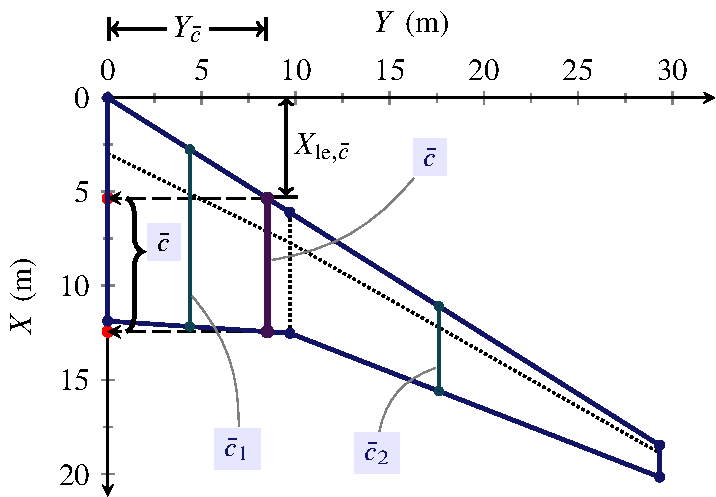
\includegraphics[width=0.78\textwidth]{exercises/wing_ac_cranked_1/wing_ac_cranked_1_drawing_mac.pdf}%
  \caption{\finalhyphendemerits=1000
           Corda media aerodinamica dell'ala proposta nell'esempio~\ref{example:Wing:Aerodynamic:Center:Cranked}.
  }
  \label{fig:Wing:Aerodynamic:Center:Cranked:MAC}%
\end%
    %{figure}%
    {SCfigure}%
%
%\EnlargedFigure% needs two latex passes
%    {t}% #1: t, b, p
%    {images/airfoil_geometry}% #2: the image file included by \includegraphics
%    {width=1.0\textwidth}% #3: option list to pass to \includegraphics, e.g. width=\linewidth,rotate=0
%    {\finalhyphendemerits=1000
%      Alcune caratteristiche geometriche di un profilo alare.}% #4: the caption text
%    {fig:Aero:Profilo:Geometria}% #5: the label
%\EnlargedFigureX% needs two latex passes
%  {t}% #1: t, b, p
%  {%
%    \begin{tabular}{@{}c@{}}
%    \makebox[\textwidth][c]{%
%      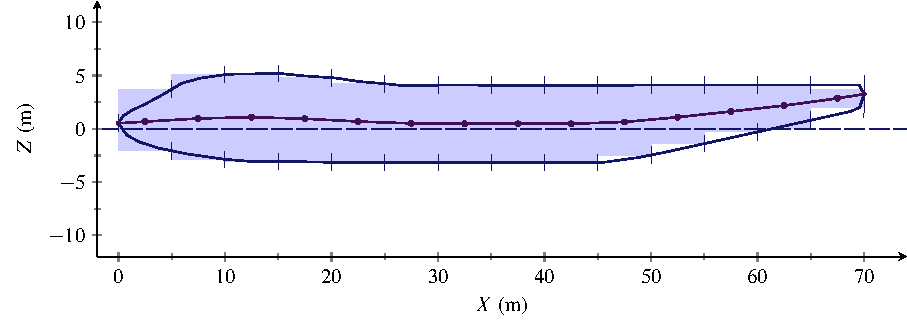
\includegraphics[width=1.00\textwidth]{exercises/fuselage_multhopp_1/fuselage_sideview_1.pdf}%
%    }% end-of-makebox
%    \\
%    \makebox[\textwidth][c]{%
%      \rule{2.2mm}{0pt}% --> hack
%      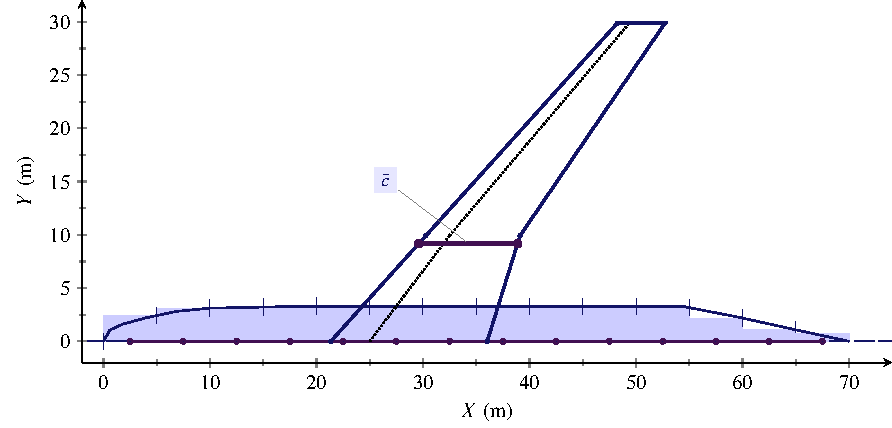
\includegraphics[width=0.98\textwidth]{exercises/fuselage_multhopp_1/fuselage_topview_1.pdf}%
%    }% end-of-makebox
%    \end{tabular}
%    \vspace{0.3cm}
%  }% #2: the image file included by \includegraphics
%  {\finalhyphendemerits=1000
%    Fusoliera assegnata nell'esempio~\ref{example:Fuselage:Multhopp:A}.
%    Discretizzazione della proiezione laterale per il calcolo approssimato dei coefficienti
%    \smash{$C_{\mathcal{M}0,\Body}$} e \smash{$C_{\mathcal{M}_\mathlarger{\alpha},\Body}$}
%    con il metodo di integrazione per strisce di Multhopp.
%  }% #3: the caption text
%  {fig:Fuselage:Multhopp:Results:AA}%% #4: the label
%
%-----------------------------------------------------------------------------------------------

Nella figura~\ref{fig:Wing:Aerodynamic:Center:Cranked:MAC}
è riportato il disegno della forma in pianta assegnata dove sono indicate le corde $\bar{c}_1$, $\bar{c}_2$ e $\bar{c}$
e le distanze $X_{\mathrm{le},\bar{c}}$ ed $Y_{\bar{c}}$.

\medskip
A questo punto si procede al calcolo del centro aerodinamico dell'ala assegnata.
Il metodo grafico utilizzato nell'esempio~\ref{example:Wing:Aerodynamic:Center:A}
per la determinazione del centro aerodinamico di un'ala a bordi dritti
può essere applicato qui a ciascuno dei due pannelli alari.
A differenza del caso di un'ala semplice, per un'ala \emph{cranked} bisogna ricavare 
un pannello 
esterno \emph{esteso} --- detto \emph{constructed outer panel} --- come mostrato nelle 
figure~\ref{fig:Wing:Aerodynamic:Center:Cranked:Panels}
e~\ref{fig:Wing:Aerodynamic:Center:Cranked:Panels:AC}. 
Esso si costruisce prolungando i bordi d'attacco
e d'uscita del pannello~2 verso l'interno,
partendo, rispettivamente, dai punti $B$ e $B'$, fino a incontrare nei punti $D$ e $D'$ la retta parallela 
all'asse $X$ di equazione $Y=\frac{1}{4}b_1$.
Pertanto, nei calcoli che seguono si considera il pannello interno
$\mathcal{P}_1=ABB'A'$ e,
al posto del pannello $\mathcal{P}_2=BCC'B$,
il pannello esterno esteso $\mathcal{P}_{2'}=DCC'D'$.

Per quanto riguarda il pannello interno $\mathcal{P}_{1}$,
dai dati e dalla figura~\ref{fig:Wing:Ac:K:One:Plots}
si legge
\[
\lambda_1=\SI[round-precision=2]{\myTaperRatioWingI}{}
%
%\quad \Longrightarrow \quad
%\quad \begin{array}{@{}c@{}} \myIconGraph \\[-4pt] \Longrightarrow \end{array} \quad
\adjustbox{center=4em}{%
  \adjustbox{lap=\width}{\raisebox{2.2ex}[0pt][0pt]{\myIconGraph}}$\Longrightarrow$%
}
%
K_{1,\mathcal{P}_{1}}
  = \mathunderline{mydarkblue}{ \SI[round-precision=3]{\myKOneACDatcomWingI}{} }
\]
dalla figura~\ref{fig:Wing:Ac:K:Two:Plots}
si legge
\[
\Lambda_\mathrm{le,1} = \SI[round-precision=1]{\mySweepLEWingIDEG}{\deg}\;,\;\,
\AR_1 = \SI[round-precision=1]{\myAspectRatioWingI}{}\;,\;\,
\lambda_1=\SI[round-precision=2]{\myTaperRatioWingI}{}
%\quad \Longrightarrow \quad
%\quad \begin{array}{@{}c@{}} \myIconGraph \\[-4pt] \Longrightarrow \end{array} \quad
\adjustbox{center=4em}{%
  \adjustbox{lap=\width}{\raisebox{2.2ex}[0pt][0pt]{\myIconGraph}}$\Longrightarrow$%
}
%
K_{2,\mathcal{P}_{1}} 
  = \mathunderline{mydarkblue}{ \SI[round-precision=3]{\myKTwoACDatcomWingI}{} }
\]
dalla figura~\ref{fig:Wing:Ac:X:AC:From:Apex:Plots}
si legge
\[
\Lambda_\mathrm{le,1} = \SI[round-precision=1]{\mySweepLEWingIDEG}{\deg}\;,\;\,
\Mach = \SI[round-precision=2]{\myMach}{}\;,\;\,
\AR_1 = \SI[round-precision=1]{\myAspectRatioWingI}{}\;,\;\,
\lambda_1=\SI[round-precision=2]{\myTaperRatioWingI}{}
%
%\quad \Longrightarrow \quad
%\quad \begin{array}{@{}c@{}} \myIconGraph \\[-4pt] \Longrightarrow \end{array} \quad
\adjustbox{center=4em}{%
  \adjustbox{lap=\width}{\raisebox{2.2ex}[0pt][0pt]{\myIconGraph}}$\Longrightarrow$%
}
%
\left.
\frac{X'_{\mathrm{ac}}}{c_\mathrm{r}}\right|_{\mathcal{P}_{1}}
  = \mathunderline{mydarkblue}{ \SI[round-precision=3]{\myXACOverChordRootDatcomWingI}{} }
\]
%
Si ottiene dunque
\[
\left.
\frac{x_{\mathrm{ac}}}{\bar{c}}\right|_{\mathcal{P}_{1}} 
  = K_{1,\mathcal{P}_{1}} 
    \left( 
      \left.\frac{X'_{\mathrm{ac}}}{c_\mathrm{r}}\right|_{\mathcal{P}_{1}} 
        - K_{2,\mathcal{P}_{1}}
    \right)
  = \SI[round-precision=3]{\myKOneACDatcomWingI}{} \,
    \Big(  
      \SI[round-precision=3]{\myXACOverChordRootDatcomWingI}{} 
        - \SI[round-precision=3]{\myKTwoACDatcomWingI}{}  
    \Big)
  = \mathunderline{mydarkblue}{ \SI[round-precision=3]{\myXsiACWingI}{} } 
\]

%-----------------------------------------------------------------------------------------------
\begin%
  %{figure}
  {SCfigure}[1.9]%
  [t]%[H]%[!htbp]
  %\centering
  %\checkoddpage
  %\centering
    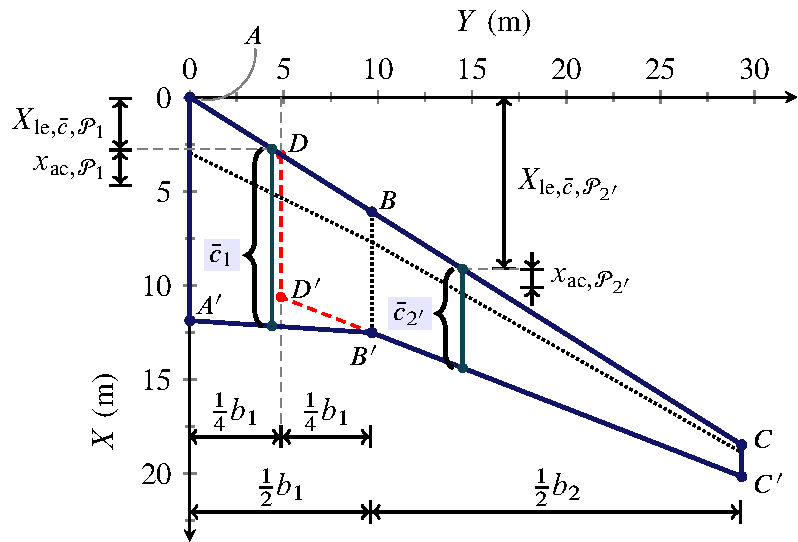
\includegraphics[width=0.78\textwidth]{exercises/wing_ac_cranked_1/wing_ac_cranked_1_drawing_panels_ac.pdf}%
  \caption{\finalhyphendemerits=1000
           Centri aerodinamici dei pannelli 
           $\mathcal{P}_1=ABB'A'$ e $\mathcal{P}_{2'}=DCC'D'$.
  }
  \label{fig:Wing:Aerodynamic:Center:Cranked:Panels:AC}%
\end%
    %{figure}%
    {SCfigure}%
%
%\EnlargedFigure% needs two latex passes
%    {t}% #1: t, b, p
%    {images/airfoil_geometry}% #2: the image file included by \includegraphics
%    {width=1.0\textwidth}% #3: option list to pass to \includegraphics, e.g. width=\linewidth,rotate=0
%    {\finalhyphendemerits=1000
%      Alcune caratteristiche geometriche di un profilo alare.}% #4: the caption text
%    {fig:Aero:Profilo:Geometria}% #5: the label
%\EnlargedFigureX% needs two latex passes
%  {t}% #1: t, b, p
%  {%
%    \begin{tabular}{@{}c@{}}
%    \makebox[\textwidth][c]{%
%      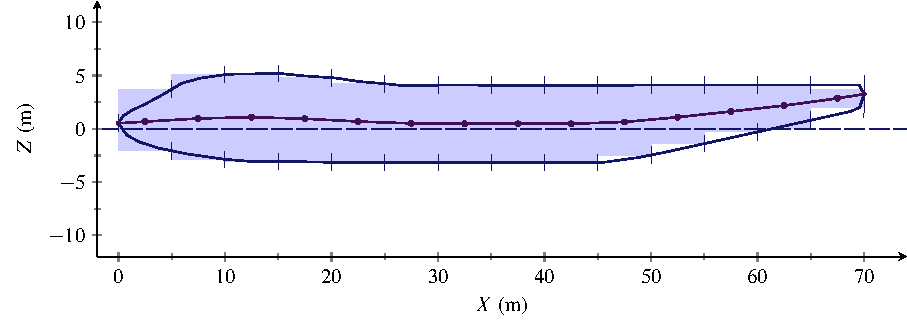
\includegraphics[width=1.00\textwidth]{exercises/fuselage_multhopp_1/fuselage_sideview_1.pdf}%
%    }% end-of-makebox
%    \\
%    \makebox[\textwidth][c]{%
%      \rule{2.2mm}{0pt}% --> hack
%      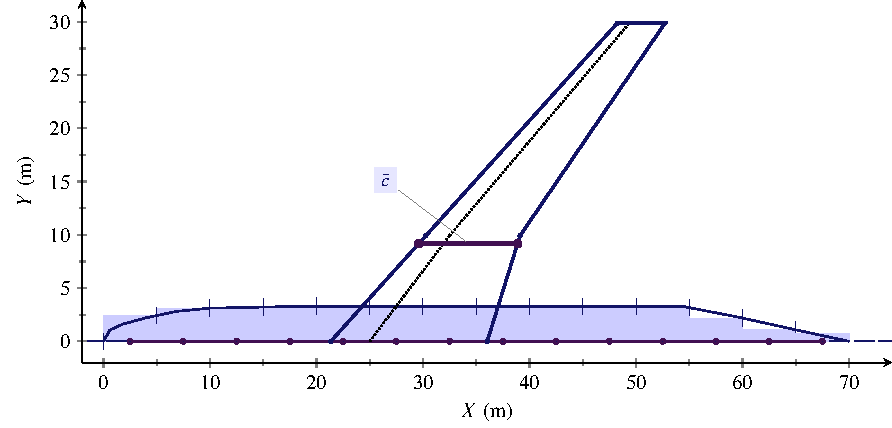
\includegraphics[width=0.98\textwidth]{exercises/fuselage_multhopp_1/fuselage_topview_1.pdf}%
%    }% end-of-makebox
%    \end{tabular}
%    \vspace{0.3cm}
%  }% #2: the image file included by \includegraphics
%  {\finalhyphendemerits=1000
%    Fusoliera assegnata nell'esempio~\ref{example:Fuselage:Multhopp:A}.
%    Discretizzazione della proiezione laterale per il calcolo approssimato dei coefficienti
%    \smash{$C_{\mathcal{M}0,\Body}$} e \smash{$C_{\mathcal{M}_\mathlarger{\alpha},\Body}$}
%    con il metodo di integrazione per strisce di Multhopp.
%  }% #3: the caption text
%  {fig:Fuselage:Multhopp:Results:AA}%% #4: the label
%
%-----------------------------------------------------------------------------------------------

Per quanto riguarda il pannello interno $\mathcal{P}_{2'}$,
si ricava
\[
b_{2'} = 2 \left( \frac{1}{2}b_2 + \frac{1}{4}b_1 \right)
  =
    2 \big(
    \calcSI[round-precision=2,fixed-exponent=0,scientific-notation=fixed]{0.5*\mySpanWingIIMT}{\metre}
    +
    \calcSI[round-precision=2,fixed-exponent=0,scientific-notation=fixed]{0.25*\mySpanWingIMT}{\metre}
    \big)
  = \SI[round-precision=2]{\mySpanWingIIPrimeMT}{m}
\]
\[
c_{\mathrm{r},2'}
  = A_{c,2} \, \bigg( - \frac{1}{4}b_1 \bigg) + B_{c,2}
  =
    \SI[round-precision=3]{\myCoeffAChordWingII}{} \, 
    \big(
      - \calcSI[round-precision=2,fixed-exponent=0,scientific-notation=fixed]{0.25*\mySpanWingIMT}{\metre}
    \big)
    + \SI[round-precision=2]{\myCoeffBChordWingIIMT}{\metre}
  = \SI[round-precision=2]{\myChordRootWingIIPrimeMT}{m}
\]
\[
\lambda_{2'}
  =\frac{c_{\mathrm{t},2}}{c_{\mathrm{r},2'}}
  =\frac{\SI[round-precision=2]{\myChordTipWingIIMT}{\metre}}{\SI[round-precision=2]{\myChordRootWingIIPrimeMT}{\metre}}
  =\mathunderline{mydarkblue}{ \SI[round-precision=2]{\myTaperRatioWingIIPrime}{} }
\]
\[
S_{2'} 
  = \frac{b_{2'}}{2} \, c_{\mathrm{r},{2'}} \, \big( 1 + \lambda_{2'} \big)
  =
    \num{0.5} \cdot \SI[round-precision=1]{\mySpanWingIIPrimeMT}{\metre}
      \cdot \SI[round-precision=2]{\myChordRootWingIIPrimeMT}{\metre}
      \cdot \big( 1 + \SI[round-precision=2]{\myTaperRatioWingIIPrime}{} \big) 
    = \mathunderline{mydarkblue}{ \SI[round-precision=1]{\myAreaWingIIPrimeMTsquared}{\metre^2} }
\]
\[
\AR_{2'} 
  = \frac{b_{2'}^2}{S_{2'}}
  = \frac{\big(\SI[round-precision=1]{\mySpanWingIIPrimeMT}{\metre}\big)^2}{\SI[round-precision=1]{\myAreaWingIIPrimeMTsquared}{\metre^2}}
  = \mathunderline{mydarkblue}{ \num[round-precision=2]{\myAspectRatioWingIIPrime} }
\]


Dai dati e dalla figura~\ref{fig:Wing:Ac:K:One:Plots}
si legge
\[
\lambda_{2'}=\SI[round-precision=2]{\myTaperRatioWingIIPrime}{}
%
%\quad \Longrightarrow \quad
%\quad \begin{array}{@{}c@{}} \myIconGraph \\[-4pt] \Longrightarrow \end{array} \quad
\adjustbox{center=4em}{%
  \adjustbox{lap=\width}{\raisebox{2.2ex}[0pt][0pt]{\myIconGraph}}$\Longrightarrow$%
}
%
K_{1,\mathcal{P}_{2'}}
  = \mathunderline{mydarkblue}{ \SI[round-precision=3]{\myKOneACDatcomWingII}{} }
\]
dalla figura~\ref{fig:Wing:Ac:K:Two:Plots}
si legge
\[
\Lambda_\mathrm{le,2} = \SI[round-precision=1]{\mySweepLEWingIIDEG}{\deg}\;,\;\,
\AR_{2'} = \SI[round-precision=1]{\myAspectRatioWingIIPrime}{}\;,\;\,
\lambda_{2'}=\SI[round-precision=2]{\myTaperRatioWingIIPrime}{}
%\quad \Longrightarrow \quad
%\quad \begin{array}{@{}c@{}} \myIconGraph \\[-4pt] \Longrightarrow \end{array} \quad
\adjustbox{center=4em}{%
  \adjustbox{lap=\width}{\raisebox{2.2ex}[0pt][0pt]{\myIconGraph}}$\Longrightarrow$%
}
%
K_{2,\mathcal{P}_{2'}} 
  = \mathunderline{mydarkblue}{ \SI[round-precision=3]{\myKTwoACDatcomWingII}{} }
\]
dalla figura~\ref{fig:Wing:Ac:X:AC:From:Apex:Plots}
si legge
\[
\Lambda_\mathrm{le,2} = \SI[round-precision=1]{\mySweepLEWingIIDEG}{\deg}\;,\;\,
\Mach = \SI[round-precision=2]{\myMach}{}\;,\;\,
\AR_{2'} = \SI[round-precision=1]{\myAspectRatioWingIIPrime}{}\;,\;\,
\lambda_{2'}=\SI[round-precision=2]{\myTaperRatioWingIIPrime}{}
%
%\quad \Longrightarrow \quad
%\quad \begin{array}{@{}c@{}} \myIconGraph \\[-4pt] \Longrightarrow \end{array} \quad
\adjustbox{center=4em}{%
  \adjustbox{lap=\width}{\raisebox{2.2ex}[0pt][0pt]{\myIconGraph}}$\Longrightarrow$%
}
%
\left.
\frac{X'_{\mathrm{ac}}}{c_\mathrm{r}}\right|_{\mathcal{P}_{2'}}
  = \mathunderline{mydarkblue}{ \SI[round-precision=3]{\myXACOverChordRootDatcomWingII}{} }
\]

A questo punto può calcolarsi la quantità
\[
\frac{X_{\mathrm{ac}}}{c_\mathrm{r}}
  = \frac{
    \left.\dfrac{X'_{\mathrm{ac}}}{c_\mathrm{r}}\right|_{\mathcal{P}_{1}}
      \, S_{1} \, C_{L_\mathlarger{\alpha}}\Big|_{\mathcal{P}_{1}}
    +
    \left.\dfrac{X'_{\mathrm{ac}}}{c_\mathrm{r}}\right|_{\mathcal{P}_{2'}}
      \, S_{2'} \, C_{L_\mathlarger{\alpha}}\Big|_{\mathcal{P}_{2'}}
  }{
    S_{1} \, C_{L_\mathlarger{\alpha}}\Big|_{\mathcal{P}_{2'}} 
    + S_{2'} \, C_{L_\mathlarger{\alpha}}\Big|_{\mathcal{P}_{2'}} 
  }
\]
dopo aver determinato per ciascun pannello il gradiente del coefficiente 
di portanza.
Per le caratteristiche geometriche dei pannelli $\mathcal{P}_{1}$ e 
$\mathcal{P}_{2'}$ si possono stimare i due gradienti come segue:
\[
C_{L_\mathlarger{\alpha}}\Big|_{\mathcal{P}_{1}}
  =
  \frac{
    a_0 \cos \Lambda_{\mathrm{le,1}}
  }{
    \sqrt{
      1 - \Mach^2 \cos^2 \Lambda_{\mathrm{le,1}}
        + \left( \dfrac{ a_0 \cos \Lambda_{\mathrm{le,1}} }{ \pi \AR_1} \right)^2
    }
    +
    \dfrac{ a_0 \cos \Lambda_{\mathrm{le,1}} }{ \pi \AR_1}
  }
\]
\[
C_{L_\mathlarger{\alpha}}\Big|_{\mathcal{P}_{2'}}
  =
  \frac{
    a_0 \cos \Lambda_{\mathrm{le,2}}
  }{
    \sqrt{
      1 - \Mach^2 \cos^2 \Lambda_{\mathrm{le,2}}
        + \left( \dfrac{ a_0 \cos \Lambda_{\mathrm{le,2}} }{ \pi \AR_{2'}} \right)^2
    }
    +
    \dfrac{ a_0 \cos \Lambda_{\mathrm{le,2}} }{ \pi \AR_{2'}}
  }
\]
con
\[
a_0 = 
  \frac{
    \SI[round-precision=3]{\myCLAlphaAtMACWingRAD}{\radian^{-1}}
  }{
    \sqrt{ 1 - \Mach^2 \cos^2 \Lambda_{\mathrm{le,1}} }
  }
  \qquad (\, \Lambda_{\mathrm{le,1}} = \Lambda_{\mathrm{le,2}} \,)
\]
Dai dati del problema è facile verificare che si ha
\[
C_{L_\mathlarger{\alpha}}\Big|_{\mathcal{P}_{1}}
  = \SI[round-precision=3]{\myCLAlphaPolhamusWingIRAD}{\radian^{-1}}
  = \SI[round-precision=4]{\myCLAlphaPolhamusWingIDEG}{\deg^{-1}}
\,,
\qquad
C_{L_\mathlarger{\alpha}}\Big|_{\mathcal{P}_{2'}}
  = \SI[round-precision=3]{\myCLAlphaPolhamusWingIIRAD}{\radian^{-1}}
  = \SI[round-precision=4]{\myCLAlphaPolhamusWingIIDEG}{\deg^{-1}}
\]
Pertanto, si ricava
\[
\frac{X_{\mathrm{ac}}}{c_\mathrm{r}}
  = \frac{
    \SI[round-precision=3]{\myXACOverChordRootDatcomWingI}{}
    \cdot \SI[round-precision=3]{\myCLAlphaPolhamusWingIRAD}{\radian^{-1}}
    \cdot \SI[round-precision=1]{\myAreaWingIMTsquared}{\metre^{2}}
    +
    \SI[round-precision=3]{\myXACOverChordRootDatcomWingII}{}
    \cdot \SI[round-precision=3]{\myCLAlphaPolhamusWingIIRAD}{\radian^{-1}}
    \cdot \SI[round-precision=1]{\myAreaWingIIPrimeMTsquared}{\metre^{2}}
  }{
    \SI[round-precision=3]{\myCLAlphaPolhamusWingIRAD}{\radian^{-1}}
    \cdot \SI[round-precision=1]{\myAreaWingIMTsquared}{\metre^{2}}
    +
    \cdot \SI[round-precision=3]{\myCLAlphaPolhamusWingIIRAD}{\radian^{-1}}
    \cdot \SI[round-precision=1]{\myAreaWingIIPrimeMTsquared}{\metre^{2}}  
  }
  = 
  \mathunderline{mydarkblue}{ \SI[round-precision=3]{\myXACOverChordRootDatcomWing}{} }
\]

Per un'ala \emph{cranked} questo è il risultato determinante, che permette di
ottenere
\[
X_{\mathrm{ac}} = \frac{X_{\mathrm{ac}}}{c_\mathrm{r}} \, c_{\mathrm{r},1}
  = \SI[round-precision=3]{\myXACOverChordRootDatcomWing}{}
    \cdot \SI[round-precision=2]{\myChordRootWingIMT}{\metre}
  = \SI[round-precision=2]{\myACWingToApexWingMT}{\metre} 
\]
cioè
\[
\frac{x_{\mathrm{ac}}}{\bar{c}}
  = 
  \frac{
    X_{\mathrm{ac}} - X_{\mathrm{le},\bar{c}}
  }{
    \bar{c}
  }
  =
  \frac{
    \SI[round-precision=2]{\myACWingToApexWingMT}{\metre}
      - \SI[round-precision=2]{\myXXMACLEToApexWingCrankedMT}{\metre}
  }{
    \SI[round-precision=2]{\myMACWingCrankedMT}{\metre}
  }
  =
  \mathunderline{mydarkblue}{ \SI[round-precision=3]{\myXsiACWing}{} }  
\]

Il centro aerodinamico di coordinate $(X_\mathrm{ac},0)$
è rappresentato nella figura~\ref{fig:Wing:Aerodynamic:Center:Cranked:Results}.

%-----------------------------------------------------------------------------------------------
\begin%
  %{figure}
  {SCfigure}[1.9]%
  [t]%[H]%[!htbp]
  %\centering
  %\checkoddpage
  %\centering
    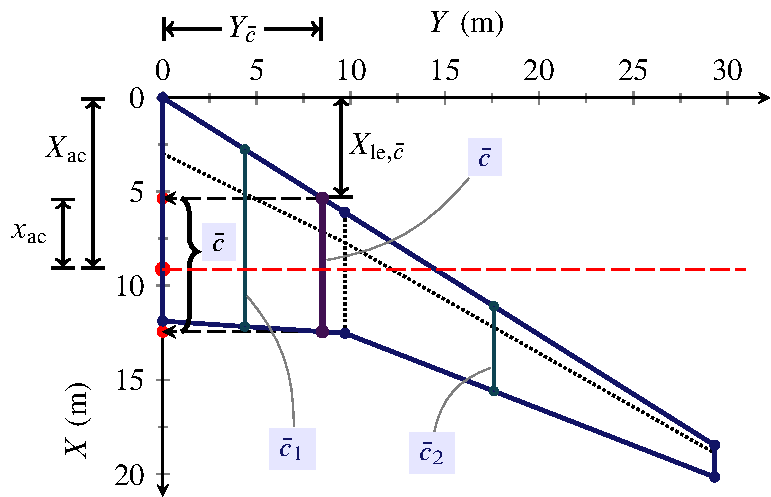
\includegraphics[width=0.78\textwidth]{exercises/wing_ac_cranked_1/wing_ac_cranked_1_drawing.pdf}%
  \caption{\finalhyphendemerits=1000
           Centro aerodinamico dell'ala proposta nell'esempio~\ref{example:Wing:Aerodynamic:Center:Cranked}. L'asse tratteggiato,
           parallelo all'asse $Y$ e passante per il centro aerodinamico alare
           è l'asse di beccheggio intorno al quale il coefficiente di momento
           dell'ala è costante al variare dell'angolo d'attacco della corrente:
           \smash{$\partial C_{\mathcal{M}_\mathlarger{\mathrm{ac}}}/\partial\alpha = 0$}.
  }
  \label{fig:Wing:Aerodynamic:Center:Cranked:Results}%
\end%
    %{figure}%
    {SCfigure}%
%
%\EnlargedFigure% needs two latex passes
%    {t}% #1: t, b, p
%    {images/airfoil_geometry}% #2: the image file included by \includegraphics
%    {width=1.0\textwidth}% #3: option list to pass to \includegraphics, e.g. width=\linewidth,rotate=0
%    {\finalhyphendemerits=1000
%      Alcune caratteristiche geometriche di un profilo alare.}% #4: the caption text
%    {fig:Aero:Profilo:Geometria}% #5: the label
%\EnlargedFigureX% needs two latex passes
%  {t}% #1: t, b, p
%  {%
%    \begin{tabular}{@{}c@{}}
%    \makebox[\textwidth][c]{%
%      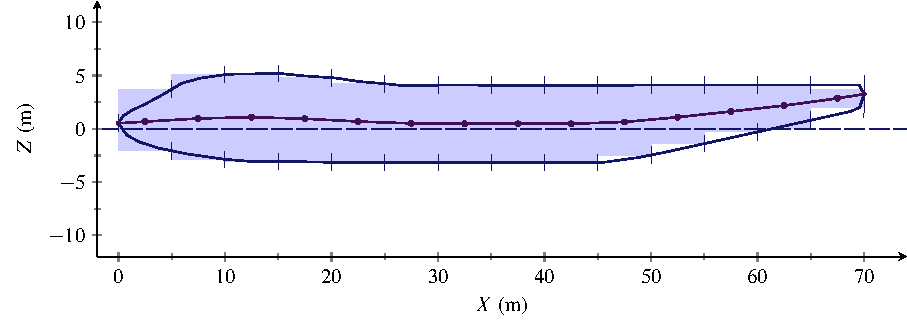
\includegraphics[width=1.00\textwidth]{exercises/fuselage_multhopp_1/fuselage_sideview_1.pdf}%
%    }% end-of-makebox
%    \\
%    \makebox[\textwidth][c]{%
%      \rule{2.2mm}{0pt}% --> hack
%      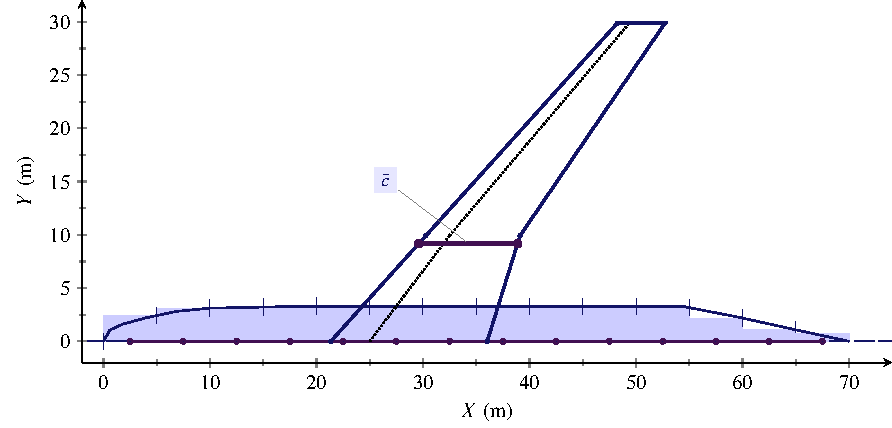
\includegraphics[width=0.98\textwidth]{exercises/fuselage_multhopp_1/fuselage_topview_1.pdf}%
%    }% end-of-makebox
%    \end{tabular}
%    \vspace{0.3cm}
%  }% #2: the image file included by \includegraphics
%  {\finalhyphendemerits=1000
%    Fusoliera assegnata nell'esempio~\ref{example:Fuselage:Multhopp:A}.
%    Discretizzazione della proiezione laterale per il calcolo approssimato dei coefficienti
%    \smash{$C_{\mathcal{M}0,\Body}$} e \smash{$C_{\mathcal{M}_\mathlarger{\alpha},\Body}$}
%    con il metodo di integrazione per strisce di Multhopp.
%  }% #3: the caption text
%  {fig:Fuselage:Multhopp:Results:AA}%% #4: the label
%
%-----------------------------------------------------------------------------------------------


\end{myExampleX}
%=END-ES===========================================================================================

%=BEGING-EX=================================================================================================
%
\def\myDummyValue{-999}
\def\myMach{0.65}
\def\myDummyValue{-999}
\def\myAreaWingMTsquared{499.17}
\def\myAreaWingFTsquared{5373.01}
\def\mySpanWingMT{59.7408}
\def\mySpanWingFT{196}
\def\myTaperRatioWing{0.305}
\def\myInducedDragFactorWing{0.9}
\def\myIncidenceWingRAD{0.03491}
\def\myIncidenceWingDEG{2}
\def\mySweepLEWingRAD{0.7330383}
\def\mySweepLEWingDEG{42}
\def\myXsiTmaxWing{0.3}
\def\mySweepTmaxWingRAD{0.6814218}
\def\mySweepTmaxWingDEG{39.04259}
\def\myDihedralWingRAD{0.08727}
\def\myDihedralWingDEG{5}
\def\myAlphaZeroLiftMeanWingRAD{-0.03743}
\def\myAlphaZeroLiftMeanWingDEG{-2.1}
\def\myThicknessOverChordMeanWing{0.12}
\def\myCmZeroMeanWing{-0.0737588}
\def\myCLAlphaMeanWingRAD{6.06584}
\def\myCLAlphaMeanWingDEG{0.10587}
\def\myChordRootWingMT{14.69}
\def\myChordRootWingFT{48.2}
\def\myChordTipWingMT{4.48}
\def\myChordTipWingFT{14.7}
\def\myRootChordWingLongitudinalPlaneMT{12.23}
\def\myRootChordWingLongitudinalPlaneFT{40.13}
\def\myXEquivalentChordLEToApexWingMT{0}
\def\myXEquivalentChordLEToApexWingFT{0}
\def\myXEquivalentChordTEToApexWingMT{12.231}
\def\myXEquivalentChordTEToApexWingFT{40.127}
\def\myEquivalentTaperRatioWing{0.366}
\def\myEquivalentSweepLEWingRAD{0.73304}
\def\myEquivalentSweepLEWingDEG{42}
\def\myEquivalentSweepQuarterChordWingRAD{0.69604}
\def\myEquivalentSweepQuarterChordWingDEG{39.88}
\def\myEquivalentSweepHalfChordWingRAD{0.6566}
\def\myEquivalentSweepHalfChordWingDEG{37.621}
\def\myEquivalentSweepTEWingRAD{0.56999}
\def\myEquivalentSweepTEWingDEG{32.658}
\def\myAspectRatioEquivalentWing{7.15}
\def\myAspectRatioWing{7.15}
\def\myMACWingMT{9.29}
\def\myMACWingFT{30.47}
\def\myXMACLEToApexWingMT{8.25}
\def\myXMACLEToApexWingFT{27.06}
\def\myAlphaZeroLiftWingRAD{-0.025009}
\def\myAlphaZeroLiftWingDEG{-1.433}
\def\myCriticalMachNumberMACWing{0.988}
\def\myCLAlphaAtMACWingRAD{6.08087}
\def\myCLAlphaAtMACWingDEG{0.1061313}
\def\myCLAlphaWingRAD{5.72254}
\def\myCLAlphaWingDEG{0.0998771}
\def\myKPolhamus{100}
\def\myCLAlphaPolhamusWingRAD{4.54711}
\def\myCLAlphaPolhamusWingDEG{0.0793621}
\def\myCmZeroAWing{-0.0737588}
\def\myCmZeroBWing{0.0532358}
\def\myCmZeroWing{-0.02052}
\def\myXMACLEToApexWingMT{8.24866}
\def\myXMACLEToApexWingFT{27.06254}
\def\myXsiACWing{0.53693}
\def\myXACOverChordRootDatcomWing{0.900896}
\def\myRiggingAngleWingRAD{0.03490659}
\def\myRiggingAngleWingDEG{2}
\def\myAreaWingIMTsquared{233.45}
\def\myAreaWingIFTsquared{2512.84}
\def\mySpanWingIMT{19.8423}
\def\mySpanWingIFT{65.0994}
\def\myTaperRatioWingI{0.602}
\def\myAspectRatioWingI{1.687}
\def\myMACWingIMT{12.008}
\def\myMACWingIFT{39.396}
\def\mySweepLEWingIRAD{0.73304}
\def\mySweepLEWingIDEG{42}
\def\mySweepTEWingIRAD{0.3011}
\def\mySweepTEWingIDEG{17.251}
\def\myTwistWingIRAD{0}
\def\myTwistWingIDEG{0}
\def\myAlphaZeroLiftRootWingIRAD{-0.04363}
\def\myAlphaZeroLiftRootWingIDEG{-2.5}
\def\myAlphaZeroLiftTipWingIRAD{-0.04363}
\def\myAlphaZeroLiftTipWingIDEG{-2.5}
\def\myAlphaZeroLiftMeanWingIRAD{-0.04363}
\def\myAlphaZeroLiftMeanWingIDEG{-2.5}
\def\myAlphaZeroLiftWingIRAD{-0.02041}
\def\myAlphaZeroLiftWingIDEG{-1.17}
\def\myThicknessOverChordRootWingI{0.15}
\def\myThicknessOverChordTipWingI{0.12}
\def\myThicknessOverChordMeanWingI{0.136}
\def\myCmZeroRootWingI{-0.08}
\def\myCmZeroTipWingI{-0.08}
\def\myCmZeroMeanWingI{-0.08}
\def\myCLAlphaRootWingIRAD{6.15}
\def\myCLAlphaRootWingIDEG{0.1073377}
\def\myCLAlphaTipWingIRAD{6.05}
\def\myCLAlphaTipWingIDEG{0.1055924}
\def\myCLAlphaMeanWingIRAD{6.1041451}
\def\myCLAlphaMeanWingIDEG{0.1065374}
\def\myCLAlphaAtMACWingIRAD{6.1041451}
\def\myCLAlphaAtMACWingIDEG{0.1065374}
\def\myKPolhamusI{100}
\def\myCLAlphaPolhamusWingIRAD{2.25978}
\def\myCLAlphaPolhamusWingIDEG{0.0394407}
\def\myChordRootWingIMT{14.69}
\def\myChordRootWingIFT{48.2}
\def\myChordTipWingIMT{8.84}
\def\myChordTipWingIFT{29}
\def\myXsiacRootWingI{0.25}
\def\myXsiacTipWingI{0.25}
\def\myCriticalMachNumberRootWingI{0.65}
\def\myCriticalMachNumberTipWingI{0.7}
\def\myXMACLEToApexWingIMT{4.096}
\def\myXMACLEToApexWingIFT{13.439}
\def\myYMACWingIMT{4.549}
\def\myYMACWingIFT{14.926}
\def\myXsiACWingI{0.55486}
\def\myKOneACDatcomWingI{1.220232}
\def\myKTwoACDatcomWingI{0.0075}
\def\myXACOverChordRootDatcomWingI{0.462221}
\def\myCoeffATwistWingIRADMT{0}
\def\myCoeffATwistWingIDEGMT{0}
\def\myCoeffATwistWingIRADFT{0}
\def\myCoeffATwistWingIDEGFT{0}
\def\myCoeffBTwistWingIRAD{0}
\def\myCoeffBTwistWingIDEG{0}
\def\myCoeffAChordWingI{-0.58987}
\def\myCoeffBChordWingIMT{14.69136}
\def\myCoeffBChordWingIFT{48.2}
\def\myCoeffAAeroTwistWingIRADMT{0}
\def\myCoeffAAeroTwistWingIDEGMT{0}
\def\myCoeffAAeroTwistWingIRADFT{0}
\def\myCoeffAAeroTwistWingIDEGFT{0}
\def\myCoeffBAeroTwistWingIRAD{-0.04363}
\def\myCoeffBAeroTwistWingIDEG{-2.5}
\def\myCoeffAPercThicknessWingIMT{-0.003024}
\def\myCoeffAPercThicknessWingIFT{-0.000922}
\def\myCoeffBPercThicknessWingI{0.15}
\def\myCoeffAClalphaWingIRADMT{-0.0100795}
\def\myCoeffAClalphaWingIRADFT{-0.0030722}
\def\myCoeffAClalphaWingIDEGMT{-0.0001759}
\def\myCoeffAClalphaWingIDEGFT{-5.36e-05}
\def\myCoeffBClalphaWingIRAD{6.15}
\def\myCoeffBClalphaWingIDEG{352.369}
\def\myCoeffACmZeroWingIMT{0}
\def\myCoeffACmZeroWingIFT{0}
\def\myCoeffBCmZeroWingI{-0.08}
\def\myCoeffAXsiACWingIMT{0}
\def\myCoeffAXsiACWingIFT{0}
\def\myCoeffBXsiACWingI{0.25}
\def\myCoeffAMachCrWingIMT{0.00504}
\def\myCoeffAMachCrWingIFT{0.001536}
\def\myCoeffBMachCrWingI{0.7}
\def\myAreaWingIIMTsquared{265.72}
\def\myAreaWingIIFTsquared{2860.18}
\def\myAreaWingIIPrimeMTsquared{358.79}
\def\myAreaWingIIPrimeFTsquared{3861.99}
\def\mySpanWingIIMT{39.8985}
\def\mySpanWingIIFT{130.9006}
\def\mySpanWingIIPrimeMT{49.81965}
\def\mySpanWingIIPrimeFT{163.4503}
\def\myAspectRatioWingII{5.991}
\def\myAspectRatioWingIIPrime{6.918}
\def\myMACWingIIMT{6.898}
\def\myMACWingIIFT{22.63}
\def\myMACWingIIPrimeMT{7.545}
\def\myMACWingIIPrimeFT{24.752}
\def\myTaperRatioWingII{0.507}
\def\myTaperRatioWingIIPrime{0.452}
\def\mySweepLEWingIIRAD{0.73304}
\def\mySweepLEWingIIDEG{42}
\def\mySweepTEWingIIRAD{0.59849}
\def\mySweepTEWingIIDEG{34.291}
\def\myTwistWingIIRAD{-0.05236}
\def\myTwistWingIIDEG{-3}
\def\myAlphaZeroLiftRootWingIIRAD{-0.04363}
\def\myAlphaZeroLiftRootWingIIDEG{-2.5}
\def\myAlphaZeroLiftTipWingIIRAD{-0.01745}
\def\myAlphaZeroLiftTipWingIIDEG{-1}
\def\myAlphaZeroLiftMeanWingIIRAD{-0.03197}
\def\myAlphaZeroLiftMeanWingIIDEG{-1.8}
\def\myAlphaZeroLiftWingIIRAD{-0.0046}
\def\myAlphaZeroLiftWingIIDEG{-0.26}
\def\myThicknessOverChordRootWingII{0.12}
\def\myThicknessOverChordTipWingII{0.09}
\def\myThicknessOverChordMeanWingII{0.107}
\def\myCmZeroRootWingII{-0.08}
\def\myCmZeroTipWingII{-0.04}
\def\myCmZeroMeanWingII{-0.0642127}
\def\myCLAlphaRootWingIIRAD{6.05}
\def\myCLAlphaRootWingIIDEG{0.1055924}
\def\myCLAlphaTipWingIIRAD{6.01}
\def\myCLAlphaTipWingIIDEG{0.1048943}
\def\myCLAlphaMeanWingIIRAD{6.03218}
\def\myCLAlphaMeanWingIIDEG{0.1052814}
\def\myCLAlphaAtMACWingIIRAD{5.9604275}
\def\myCLAlphaAtMACWingIIDEG{0.1040291}
\def\myKPolhamusII{100}
\def\myCLAlphaPolhamusWingIIRAD{4.50859}
\def\myCLAlphaPolhamusWingIIDEG{0.0786898}
\def\myChordRootWingIIMT{8.84}
\def\myChordRootWingIIFT{29}
\def\myChordTipWingIIMT{4.48}
\def\myChordTipWingIIFT{14.7}
\def\myXsiacRootWingII{0.25}
\def\myXsiacTipWingII{0.25}
\def\myCriticalMachNumberRootWingII{0.7}
\def\myCriticalMachNumberTipWingII{0.7}
\def\myXMACLEToApexWingIIMT{8.002}
\def\myXMACLEToApexWingIIFT{26.252}
\def\myYMACWingIIMT{8.887}
\def\myYMACWingIIFT{29.156}
\def\myXsiACWingII{0.11269}
\def\myKOneACDatcomWingII{1.311488}
\def\myKTwoACDatcomWingII{1.008142}
\def\myXACOverChordRootDatcomWingII{1.094066}
\def\myCoeffATwistWingIIRADMT{-0.002625}
\def\myCoeffATwistWingIIDEGMT{-0.15038}
\def\myCoeffATwistWingIIRADFT{-0.0008}
\def\myCoeffATwistWingIIDEGFT{-0.0458363}
\def\myCoeffBTwistWingIIRAD{0}
\def\myCoeffBTwistWingIIDEG{0}
\def\myCoeffAChordWingII{-0.21849}
\def\myCoeffBChordWingIIMT{8.8392}
\def\myCoeffBChordWingIIFT{29}
\def\myCoeffAAeroTwistWingIIRADMT{0.001312}
\def\myCoeffAAeroTwistWingIIDEGMT{0.07519}
\def\myCoeffAAeroTwistWingIIRADFT{0.0004}
\def\myCoeffAAeroTwistWingIIDEGFT{0}
\def\myCoeffBAeroTwistWingIIRAD{-0.04363}
\def\myCoeffBAeroTwistWingIIDEG{-2.5}
\def\myCoeffAPercThicknessWingIIMT{-0.001504}
\def\myCoeffAPercThicknessWingIIFT{-0.000458}
\def\myCoeffBPercThicknessWingII{0.12}
\def\myCoeffAClalphaWingIIRADMT{-0.0020051}
\def\myCoeffAClalphaWingIIRADFT{-0.0006112}
\def\myCoeffAClalphaWingIIDEGMT{-3.5e-05}
\def\myCoeffAClalphaWingIIDEGFT{-1.07e-05}
\def\myCoeffBClalphaWingIIRAD{6.05}
\def\myCoeffBClalphaWingIIDEG{346.639}
\def\myCoeffACmZeroWingIIMT{0.0020051}
\def\myCoeffACmZeroWingIIFT{0.0006112}
\def\myCoeffBCmZeroWingII{-0.08}
\def\myCoeffAXsiACWingIIMT{0}
\def\myCoeffAXsiACWingIIFT{0}
\def\myCoeffBXsiACWingII{0.25}
\def\myCoeffAMachCrWingIIMT{0}
\def\myCoeffAMachCrWingIIFT{0}
\def\myCoeffBMachCrWingII{0.7}
\def\myAreaWingCrankedMTsquared{499.17}
\def\myAreaWingCrankedFTsquared{5373.01}
\def\myMACWingCrankedMT{9.28755}
\def\myMACWingCrankedFT{30.47096}
\def\myAspectRatioWingCranked{7.15}
\def\myXMACLEToApexWingCrankedMT{6.17513}
\def\myXMACLEToApexWingCrankedFT{20.2596}
\def\myXXMACLEToApexWingCrankedMT{8.24866}
\def\myXXMACLEToApexWingCrankedFT{27.06254}
\def\myYMACWingCrankedMT{6.85817}
\def\myYMACWingCrankedFT{22.50056}
\def\myYYMACWingCrankedMT{9.16107}
\def\myYYMACWingCrankedFT{30.05599}

%
\begin{myExerciseX}{Centro aerodinamico dell'ala di un Boeing~747}{\ding{46}\ \myIconGraph\ }% \ \Keyboard\ %
\label{exercise:Wing:Aerodynamic:Center:Cranked}
%
\noindent
Sulla base dell'esempio~\ref{example:Wing:Aerodynamic:Center:Cranked} determinare
il centro aerodinamico di un'ala simile a quella di un Boeing~747.
La forma in pianta assegnata è rappresentata nella
figura~\ref{fig:Wing:Aerodynamic:Center:Cranked:B747:Topview}
e possiede le seguenti caratteristiche:

\smallskip
\noindent
\adjustbox{center=\textwidth}{%
 \underline{\emph{Pannello 1} (pannello interno)}
}

\smallskip
\noindent
\adjustbox{left=\textwidth}{%
  \adjustbox{right=0.39\textwidth}{%
    \emph{corde}:
  }\rule{0.5em}{0pt}% --> SPACER
  \adjustbox{left=0.59\textwidth}{%
    $c_{\mathrm{r},1}=\SI[round-precision=2]{\myChordRootWingIMT}{\metre}$,
    $c_{\mathrm{t},1}=\SI[round-precision=2]{\myChordTipWingIMT}{\metre}$,
    $\lambda_1 = \SI[round-precision=2]{\myTaperRatioWingI}{}$,
  }%
}

\smallskip
\noindent
\adjustbox{left=\textwidth}{%
  \adjustbox{right=0.39\textwidth}{%
    \emph{apertura e superficie}:
  }\rule{0.5em}{0pt}% --> SPACER
  \adjustbox{left=0.59\textwidth}{%
    $b_1=\SI[round-precision=2]{\mySpanWingIMT}{\metre}$,
    $S_1=\SI[round-precision=2]{\myAreaWingIMTsquared}{\meter^2}$,
    $\AR_1 = \SI[round-precision=2]{\myAspectRatioWingI}{}$,
  }%
}

\smallskip
\noindent
\adjustbox{left=\textwidth}{%
  \adjustbox{right=0.39\textwidth}{%
    \emph{angoli di freccia}:
  }\rule{0.5em}{0pt}% --> SPACER
  \adjustbox{left=0.59\textwidth,minipage=[t]{0.59\textwidth}}{%
    $\Lambda_\mathrm{le,1}=\SI[round-precision=4]{\mySweepLEWingIRAD}{\radian}=\SI[round-precision=1]{\mySweepLEWingIDEG}{\deg}$,
    \\
    $\Lambda_\mathrm{te,1}=\SI[round-precision=4]{\mySweepTEWingIRAD}{\radian}=\SI[round-precision=1]{\mySweepTEWingIDEG}{\deg}$,
  }%
}

\smallskip
\noindent
\adjustbox{left=\textwidth}{%
  \adjustbox{right=0.39\textwidth}{%
    \emph{gradienti $C_{\ell_\mathlarger{\alpha}}$ di profilo}:
  }\rule{0.5em}{0pt}% --> SPACER
  \adjustbox{left=0.59\textwidth,minipage=[t]{0.59\textwidth}}{%
    $C_{\ell_\mathlarger{\alpha},\mathrm{r},1}=\SI[round-precision=2]{\myCLAlphaRootWingIRAD}{\radian^{-1}}=\SI[round-precision=4]{\myCLAlphaRootWingIDEG}{\deg^{-1}}$,
    \\
    $C_{\ell_\mathlarger{\alpha},\mathrm{t},1}=\SI[round-precision=2]{\myCLAlphaTipWingIRAD}{\radian^{-1}}=\SI[round-precision=4]{\myCLAlphaTipWingIDEG}{\deg^{-1}}$,
  }%
}

\smallskip
\noindent
\adjustbox{left=\textwidth}{%
  \adjustbox{right=0.39\textwidth}{%
    \emph{svergolamenti}:
  }\rule{0.5em}{0pt}% --> SPACER
  \adjustbox{left=0.59\textwidth,minipage=[t]{0.59\textwidth}}{%
    $\alpha_{0\ell,\mathrm{r},1}=\SI[round-precision=3]{\myAlphaZeroLiftRootWingIRAD}{\radian}
      =\SI[round-precision=1]{\myAlphaZeroLiftRootWingIDEG}{\deg}$,\\
    $\alpha_{0\ell,\mathrm{t},1}=\SI[round-precision=3]{\myAlphaZeroLiftTipWingIRAD}{\radian}
      =\SI[round-precision=1]{\myAlphaZeroLiftTipWingIDEG}{\deg}$,\\
    $\epsilon_{\mathrm{g,t},1}=\SI[round-precision=3]{\myTwistWingIRAD}{\radian}
      =\SI[round-precision=1]{\myTwistWingIDEG}{\deg}$,
  }%
}

\smallskip
\noindent
\adjustbox{left=\textwidth}{%
  \adjustbox{right=0.39\textwidth}{%
    \emph{centri aerodinamici di profilo}:
  }\rule{0.5em}{0pt}% --> SPACER
  \adjustbox{left=0.59\textwidth}{%
    $\bar{x}_{\mathrm{ac,2D,1},\mathrm{r}}=\SI[round-precision=2]{\myXsiacRootWingI}{}$,
    $\bar{x}_{\mathrm{ac,2D,1},\mathrm{t}}=\SI[round-precision=2]{\myXsiacTipWingI}{}$,
  }%
}

\smallskip
\noindent
\adjustbox{left=\textwidth}{%
  \adjustbox{right=0.39\textwidth}{%
    \emph{coefficienti $C_{\mathcal{m}_\mathlarger{\mathrm{ac}}}$ di profilo}:
  }\rule{0.5em}{0pt}% --> SPACER
  \adjustbox{left=0.59\textwidth}{%
    $C_{\mathcal{m}_\mathlarger{\mathrm{ac}},\mathrm{r},1}=\SI[round-precision=3]{\myCmZeroRootWingI}{}$,
    $C_{\mathcal{m}_\mathlarger{\mathrm{ac}},\mathrm{t},1}=\SI[round-precision=3]{\myCmZeroTipWingI}{}$,
  }%
}

\medskip
\noindent
\adjustbox{center=\textwidth}{%
 \underline{\emph{Pannello 2} (pannello esterno)}
}

\smallskip
\noindent
\adjustbox{left=\textwidth}{%
  \adjustbox{right=0.39\textwidth}{%
    \emph{corde}:
  }\rule{0.5em}{0pt}% --> SPACER
  \adjustbox{left=0.59\textwidth}{%
    $c_{\mathrm{r},2}=\SI[round-precision=2]{\myChordRootWingIIMT}{\metre}$,
    $c_{\mathrm{t},2}=\SI[round-precision=2]{\myChordTipWingIIMT}{\metre}$,
    $\lambda_2 = \SI[round-precision=2]{\myTaperRatioWingII}{}$,
  }%
}

\smallskip
\noindent
\adjustbox{left=\textwidth}{%
  \adjustbox{right=0.39\textwidth}{%
    \emph{apertura e superficie}:
  }\rule{0.5em}{0pt}% --> SPACER
  \adjustbox{left=0.59\textwidth}{%
    $b_2=\SI[round-precision=2]{\mySpanWingIIMT}{\metre}$,
    $S_2=\SI[round-precision=2]{\myAreaWingIIMTsquared}{\meter^2}$,
    $\AR_2 = \SI[round-precision=2]{\myAspectRatioWingII}{}$,
  }%
}

\smallskip
\noindent
\adjustbox{left=\textwidth}{%
  \adjustbox{right=0.39\textwidth}{%
    \emph{angoli di freccia}:
  }\rule{0.5em}{0pt}% --> SPACER
  \adjustbox{left=0.59\textwidth,minipage=[t]{0.59\textwidth}}{%
    $\Lambda_\mathrm{le,2}=\SI[round-precision=4]{\mySweepLEWingIIRAD}{\radian}=\SI[round-precision=1]{\mySweepLEWingIIDEG}{\deg}$,
    \\
    $\Lambda_\mathrm{te,2}=\SI[round-precision=4]{\mySweepTEWingIIRAD}{\radian}=\SI[round-precision=1]{\mySweepTEWingIIDEG}{\deg}$,
  }%
}

\smallskip
\noindent
\adjustbox{left=\textwidth}{%
  \adjustbox{right=0.39\textwidth}{%
    \emph{gradienti $C_{\ell_\mathlarger{\alpha}}$ di profilo}:
  }\rule{0.5em}{0pt}% --> SPACER
  \adjustbox{left=0.59\textwidth,minipage=[t]{0.59\textwidth}}{%
    $C_{\ell_\mathlarger{\alpha},\mathrm{r},2}=\SI[round-precision=2]{\myCLAlphaRootWingIIRAD}{\radian^{-1}}=\SI[round-precision=4]{\myCLAlphaRootWingIIDEG}{\deg^{-1}}$,
    \\
    $C_{\ell_\mathlarger{\alpha},\mathrm{t},2}=\SI[round-precision=2]{\myCLAlphaTipWingIIRAD}{\radian^{-1}}=\SI[round-precision=4]{\myCLAlphaTipWingIIDEG}{\deg^{-1}}$,
  }%
}

\smallskip
\noindent
\adjustbox{left=\textwidth}{%
  \adjustbox{right=0.39\textwidth}{%
    \emph{svergolamenti}:
  }\rule{0.5em}{0pt}% --> SPACER
  \adjustbox{left=0.59\textwidth,minipage=[t]{0.59\textwidth}}{%
    $\alpha_{0\ell,\mathrm{r},2}=\SI[round-precision=3]{\myAlphaZeroLiftRootWingIIRAD}{\radian}
      =\SI[round-precision=1]{\myAlphaZeroLiftRootWingIIDEG}{\deg}$,\\
    $\alpha_{0\ell,\mathrm{t},2}=\SI[round-precision=3]{\myAlphaZeroLiftTipWingIIRAD}{\radian}
      =\SI[round-precision=1]{\myAlphaZeroLiftTipWingIIDEG}{\deg}$,\\
    $\epsilon_{\mathrm{g,t},2}=\SI[round-precision=3]{\myTwistWingIIRAD}{\radian}
      =\SI[round-precision=1]{\myTwistWingIIDEG}{\deg}$,
  }%
}

\smallskip
\noindent
\adjustbox{left=\textwidth}{%
  \adjustbox{right=0.39\textwidth}{%
    \emph{centri aerodinamici di profilo}:
  }\rule{0.5em}{0pt}% --> SPACER
  \adjustbox{left=0.59\textwidth}{%
    $\bar{x}_{\mathrm{ac,2D,2},\mathrm{r}}=\SI[round-precision=2]{\myXsiacRootWingII}{}$,
    $\bar{x}_{\mathrm{ac,2D,2},\mathrm{t}}=\SI[round-precision=2]{\myXsiacTipWingII}{}$,
  }%
}

\smallskip
\noindent
\adjustbox{left=\textwidth}{%
  \adjustbox{right=0.39\textwidth}{%
    \emph{coefficienti $C_{\mathcal{m}_\mathlarger{\mathrm{ac}}}$ di profilo}:
  }\rule{0.5em}{0pt}% --> SPACER
  \adjustbox{left=0.59\textwidth}{%
    $C_{\mathcal{m}_\mathlarger{\mathrm{ac}},\mathrm{r},2}=\SI[round-precision=3]{\myCmZeroRootWingII}{}$,
    $C_{\mathcal{m}_\mathlarger{\mathrm{ac}},\mathrm{t},2}=\SI[round-precision=3]{\myCmZeroTipWingII}{}$,
  }%
}

\medskip
\noindent
\adjustbox{left=\textwidth}{%
  \adjustbox{right=0.39\textwidth}{%
    \emph{condizione di volo}:
  }\rule{0.5em}{0pt}% --> SPACER
  \adjustbox{left=0.59\textwidth}{%
    $\Mach = \SI[round-precision=2]{\myMach}{}$.
  }%
}

%-----------------------------------------------------------------------------------------------
%\begin%
%  %{figure}
%  {SCfigure}[1.9]%
%  [t]%[H]%[!htbp]
%  %\centering
%  %\checkoddpage
%  %\centering
%    \includegraphics[width=0.88\textwidth]{exercises/wing_ac_B747/wing_B747_topview_1.pdf}%
%  \caption{\finalhyphendemerits=1000
%           Vista in pianta dell'ala di un Boeing~747. Si veda 
%           l'esercizio~\ref{exercise:Wing:Aerodynamic:Center:Cranked}.
%  }
%  \label{fig:Wing:Aerodynamic:Center:Cranked:B747:Topview}%
%\end%
%    %{figure}%
%    {SCfigure}%
%
%\EnlargedFigure% needs two latex passes
%    {t}% #1: t, b, p
%    {images/airfoil_geometry}% #2: the image file included by \includegraphics
%    {width=1.0\textwidth}% #3: option list to pass to \includegraphics, e.g. width=\linewidth,rotate=0
%    {\finalhyphendemerits=1000
%      Alcune caratteristiche geometriche di un profilo alare.}% #4: the caption text
%    {fig:Aero:Profilo:Geometria}% #5: the label
\EnlargedFigureX% needs two latex passes
  {t}% #1: t, b, p
  {%
    %\begin{tabular}{@{}c@{}}
    \makebox[\textwidth][c]{%
      \includegraphics[width=1.00\textwidth]{exercises/wing_ac_B747/wing_B747_topview_1.pdf}%
    }% end-of-makebox
    %\end{tabular}
    %\vspace{0.3cm}
  }% #2: the image file included by \includegraphics
  {\finalhyphendemerits=1000
    Vista in pianta dell'ala di un Boeing~747.
    Si veda l'esercizio~\ref{exercise:Wing:Aerodynamic:Center:Cranked}.
  }% #3: the caption text
  {fig:Wing:Aerodynamic:Center:Cranked:B747:Topview}%% #4: the label
%
%-----------------------------------------------------------------------------------------------

\medskip
Verificare che
\[
\alpha_{0L,\Wing} %= \SI[round-precision=4]{\myAlphaZeroLiftWingRAD}{rad}
  = \mathunderline{mydarkblue}{ \SI[round-precision=1]{\myAlphaZeroLiftWingDEG}{deg} }
\]
\[
\bar{c}
    = \mathunderline{mydarkblue}{ \SI[round-precision=2]{\myMACWingCrankedMT}{\metre} }
\,,\qquad  
Y_{\bar{c}} 
    = \mathunderline{mydarkblue}{
      \SI[round-precision=2]{\myYYMACWingCrankedMT}{\metre}
    }
\,,\qquad
X_{\mathrm{le},\bar{c}} 
	= \mathunderline{mydarkblue}{ \SI[round-precision=2]{\myXXMACLEToApexWingCrankedMT}{\metre} }
\]
che
\[
\frac{X_{\mathrm{ac}}}{c_\mathrm{r}}
  = 
  \mathunderline{mydarkblue}{ \SI[round-precision=3]{\myXACOverChordRootDatcomWing}{} }
\,,\qquad
X_{\mathrm{ac}}
  = 
  \mathunderline{mydarkblue}{ \SI[round-precision=2]{\myACWingToApexWingMT}{\metre} }
\]
e infine
\[
\frac{x_{\mathrm{ac}}}{\bar{c}}
  =
  \mathunderline{mydarkblue}{ \SI[round-precision=3]{\myXsiACWing}{} }  
\]

\end{myExerciseX}
%=END-EX====================================================================================================


%=BEGING-ES===========================================================================================
%
\def\mySpanWingMT{10.600000}
\def\mySpanWingIMT{6.360000}
\def\mySpanWingIIMT{4.240000}
\def\myChordRootWingMT{1.440000}
\def\myChordRootWingIMT{1.440000}
\def\myChordRootWingIIMT{1.440000}
\def\myChordTipWingMT{0.860000}
\def\myChordTipWingIMT{1.440000}
\def\myChordTipWingIIMT{0.860000}
\def\mySweepLEWingIIDEG{0.000000}
\def\myCoeffAChordWingI{0.000000}
\def\myCoeffBChordWingIMT{1.440000}
\def\myCoeffAChordWingII{-0.273585}
\def\myCoeffBChordWingIIMT{1.440000}
\def\myAlphaZeroLiftRootWingIDEG{-2.500000}
\def\myAlphaZeroLiftTipWingIDEG{-2.500000}
\def\myAlphaZeroLiftRootWingIRAD{-0.043633}
\def\myAlphaZeroLiftTipWingIRAD{-0.043633}
\def\myAlphaZeroLiftRootWingIIDEG{-2.500000}
\def\myAlphaZeroLiftTipWingIIDEG{-1.000000}
\def\myAlphaZeroLiftRootWingIIRAD{-0.043633}
\def\myAlphaZeroLiftTipWingIIRAD{-0.017453}
\def\myTaperRatioWingI{1.000000}
\def\myTaperRatioWingII{0.597222}
\def\myTwistWingIDEG{0.000000}
\def\myTwistWingIRAD{0.000000}
\def\myTwistWingIIDEG{-3.000000}
\def\myTwistWingIIRAD{-0.052360}
\def\myAreaWingIMTsquared{9.158400}
\def\myAreaWingIIMTsquared{4.876000}
\def\myAreaWingMTsquared{14.034400}
\def\myCoeffAAeroTwistWingIRADMT{0.000000}
\def\myCoeffBAeroTwistWingIRAD{-0.043633}
\def\myCoeffAAeroTwistWingIIRADMT{0.012349}
\def\myCoeffBAeroTwistWingIIRAD{-0.043633}
\def\myCoeffATwistWingIRADMT{0.000000}
\def\myCoeffATwistWingIIRADMT{-0.024698}
\def\myCoeffBTwistWingIRAD{0.000000}
\def\myCoeffBTwistWingIIRAD{0.000000}
\def\myAlphaZeroLiftWingIRAD{-0.028653}
\def\myAlphaZeroLiftWingIDEG{-1.641680}
\def\myAlphaZeroLiftWingIIRAD{0.008329}
\def\myAlphaZeroLiftWingIIDEG{0.477233}
\def\myAlphaZeroLiftWingRAD{-0.020323}
\def\myAlphaZeroLiftWingDEG{-1.164447}

%
\begin{myExampleX}{Momento di beccheggio intorno al centro aerodinamico dell'ala}{\ding{46}}% \ \Keyboard\ %
\label{example:Wing:Cmac:A}
%
\noindent
Si consideri l'ala a bordi dritti rappresentata nella figura~\ref{fig:Wing:Cmac:Results:A}
per la quale è nullo l'angolo di freccia del bordo d'attacco, 
cioè $\Lambda_\mathrm{le}=\SI[round-precision=0]{\mySweepLEWingDEG}{\deg}$.
Le rimanenti caratteristiche della superficie portante sono le seguenti:

\smallskip
\noindent
\adjustbox{left=\textwidth}{%
  \adjustbox{right=0.39\textwidth}{%
    \emph{corde}:
  }\rule{0.5em}{0pt}% --> SPACER
  \adjustbox{left=0.59\textwidth}{%
    $c_\mathrm{r}=\SI[round-precision=2]{\myChordRootWingMT}{\metre}$,
    $c_\mathrm{t}=\SI[round-precision=2]{\myChordTipWingMT}{\metre}$,
    $\lambda = \SI[round-precision=2]{\myTaperRatioWing}{}$,
  }%
}

\smallskip
\noindent
\adjustbox{left=\textwidth}{%
  \adjustbox{right=0.39\textwidth}{%
    \emph{apertura e superficie}:
  }\rule{0.5em}{0pt}% --> SPACER
  \adjustbox{left=0.59\textwidth}{%
    $b=\SI[round-precision=2]{\mySpanWingMT}{\metre}$,
    $S=\SI[round-precision=2]{\myAreaWingMTsquared}{\meter^2}$,
    $\AR = \SI[round-precision=2]{\myAspectRatioWing}{}$,
  }%
}

\smallskip
\noindent
\adjustbox{left=\textwidth}{%
  \adjustbox{right=0.39\textwidth}{%
    \emph{gradienti $C_{\ell_\mathlarger{\alpha}}$ di profilo}:
  }\rule{0.5em}{0pt}% --> SPACER
  \adjustbox{left=0.59\textwidth,minipage=[t]{0.59\textwidth}}{%
    $C_{\ell_\mathlarger{\alpha},\mathrm{r}}=\SI[round-precision=2]{\myCLAlphaRootWingRAD}{\radian^{-1}}=\SI[round-precision=4]{\myCLAlphaRootWingDEG}{\deg^{-1}}$,
    \\
    $C_{\ell_\mathlarger{\alpha},\mathrm{t}}=\SI[round-precision=2]{\myCLAlphaTipWingRAD}{\radian^{-1}}=\SI[round-precision=4]{\myCLAlphaTipWingDEG}{\deg^{-1}}$,
  }%
}

\smallskip
\noindent
\adjustbox{left=\textwidth}{%
  \adjustbox{right=0.39\textwidth}{%
    \emph{angoli di portanza nulla}:
  }\rule{0.5em}{0pt}% --> SPACER
  \adjustbox{left=0.59\textwidth,minipage=[t]{0.59\textwidth}}{%
    $\alpha_{0\ell,\mathrm{r}}=\SI[round-precision=3]{\myAlphaZeroLiftRootWingRAD}{\radian}
      =\SI[round-precision=1]{\myAlphaZeroLiftRootWingDEG}{\deg}$,\\
    $\alpha_{0\ell,\mathrm{t}}=\SI[round-precision=3]{\myAlphaZeroLiftTipWingRAD}{\radian}
      =\SI[round-precision=1]{\myAlphaZeroLiftTipWingDEG}{\deg}$,
  }%
}

\smallskip
\noindent
\adjustbox{left=\textwidth}{%
  \adjustbox{right=0.39\textwidth}{%
    \emph{centri aerodinamici di profilo}:
  }\rule{0.5em}{0pt}% --> SPACER
  \adjustbox{left=0.59\textwidth}{%
    $\bar{x}_{\mathrm{ac,2D},\mathrm{r}}=\SI[round-precision=2]{\myXsiacRootWing}{}$,
    $\bar{x}_{\mathrm{ac,2D},\mathrm{t}}=\SI[round-precision=2]{\myXsiacTipWing}{}$,
  }%
}

\smallskip
\noindent
\adjustbox{left=\textwidth}{%
  \adjustbox{right=0.39\textwidth}{%
    \emph{coefficienti $C_{\mathcal{m}_\mathlarger{\mathrm{ac}}}$ di profilo}:
  }\rule{0.5em}{0pt}% --> SPACER
  \adjustbox{left=0.59\textwidth}{%
    $C_{\mathcal{m}_\mathlarger{\mathrm{ac}},\mathrm{r}}=\SI[round-precision=3]{\myCmZeroRootWing}{}$,
    $C_{\mathcal{m}_\mathlarger{\mathrm{ac}},\mathrm{t}}=\SI[round-precision=3]{\myCmZeroTipWing}{}$,
  }%
}

\smallskip
\noindent
\adjustbox{left=\textwidth}{%
  \adjustbox{right=0.39\textwidth}{%
    \emph{condizione di volo}:
  }\rule{0.5em}{0pt}% --> SPACER
  \adjustbox{left=0.59\textwidth}{%
    $\Mach = \SI[round-precision=2]{\myMach}{}$.
  }%
}

\smallskip
Per l'ala assegnata si vuole calcolare il coefficiente \smash{$C_{\mathcal{M}_\mathlarger{\mathrm{ac}}}$}.

\medskip
L'angolo di freccia della linea dei quarti di corda --- linea che coincide in questo caso con la linea dei
fuochi delle sezioni alari --- si calcola come segue:
\[
\begin{split}
\tan
\Lambda_{c/4}
   = \tan\Lambda_\mathrm{le}-\dfrac{(4/4)(1-\lambda)}{\AR(1+\lambda)}
   & {}=
    \tan (\SI[round-precision=3]{\mySweepLEWingRAD}{\radian})
      - \dfrac{
         \num[round-precision=2]{1.0}
         \cdot (1-\SI[round-precision=2]{\myTaperRatioWing}{})
      }{
         \num[round-precision=2]{\myAspectRatioWing}
         \cdot (1+\SI[round-precision=2]{\myTaperRatioWing}{})} 
\\[3pt]
   & \Rightarrow
   \quad
   \Lambda_{c/4}
      = \mathunderline{mydarkblue}{ \SI[round-precision=4]{\mySweepQuarterChordWingRAD}{\radian} }
      = \mathunderline{mydarkblue}{ \SI[round-precision=1]{\mySweepQuarterChordWingDEG}{\deg} }
\end{split}
\]
L'ala assegnata ha dunque un angolo di freccia $\Lambda_{c/4}$ piccolo e negativo.

La corda media aerodinamica è in questo caso
\[
\bar{c} = \frac{2}{3} \, c_\mathrm{r} \, \frac{1+\lambda + \lambda^2}{1+\lambda}
  =
    \num{0.667} \cdot \SI[round-precision=2]{\myChordRootWingMT}{\metre}
      \cdot 
        \frac{
          1 + \SI[round-precision=2]{\myTaperRatioWing}{} + \SI[round-precision=2]{\myTaperRatioWing}{}^2
        }{
          1 + \SI[round-precision=2]{\myTaperRatioWing}{}
        }
    = \mathunderline{mydarkblue}{ \SI[round-precision=2]{\myMACWingMT}{\metre} }
\]

La distanza longitudinale del bordo d'attacco della corda media aerodinamica dal
bordo d'attacco della corda di radice è nulla, 
$X_{\mathrm{le},\bar{c}} = \SI[round-precision=2]{\myXMACLEToApexWingMT}{\metre}$, 
essendo nullo l'angolo $\Lambda_\mathrm{le}$.

La stazione $Y_{\bar{c}}$ alla quale la legge delle corde $c(Y)$ assume il valore $\bar{c}$ è
\[
Y_{\bar{c}} 
  =
    \frac{b}{6} \, \frac{1+2\lambda}{1+\lambda}
  =
    \frac{\SI[round-precision=1]{\mySpanWingMT}{\metre}}{6}
      \cdot 
      \frac{
        1 + 2\cdot\SI[round-precision=2]{\myTaperRatioWing}{}
      }{
        1 + \SI[round-precision=2]{\myTaperRatioWing}{}
      }
    = \mathunderline{mydarkblue}{ \SI[round-precision=2]{\myYMACWingMT}{\metre} }
\]


Per il numero di Mach di volo assegnato
il centro aerodinamico dell'ala si calcola come nell'esempio~\ref{example:Wing:Aerodynamic:Center:A}.
Dai dati e dalla figura~\ref{fig:Wing:Ac:K:One:Plots}
si legge
\[
\lambda=\SI[round-precision=2]{\myTaperRatioWing}{}
%
%\quad \Longrightarrow \quad
%\quad \begin{array}{@{}c@{}} \myIconGraph \\[-4pt] \Longrightarrow \end{array} \quad
\adjustbox{center=4em}{%
  \adjustbox{lap=\width}{\raisebox{2.2ex}[0pt][0pt]{\myIconGraph}}$\Longrightarrow$%
}
%
K_1
  = \mathunderline{mydarkblue}{ \SI[round-precision=3]{\myKOneACDatcomWing}{} }
\]
dalla figura~\ref{fig:Wing:Ac:K:Two:Plots}
si legge
\[
\Lambda_\mathrm{le} = \SI[round-precision=1]{\mySweepLEWingDEG}{\deg}\;,\;\,
\AR = \SI[round-precision=1]{\myAspectRatioWing}{}\;,\;\,
\lambda=\SI[round-precision=2]{\myTaperRatioWing}{}
%\quad \Longrightarrow \quad
%\quad \begin{array}{@{}c@{}} \myIconGraph \\[-4pt] \Longrightarrow \end{array} \quad
\adjustbox{center=4em}{%
  \adjustbox{lap=\width}{\raisebox{2.2ex}[0pt][0pt]{\myIconGraph}}$\Longrightarrow$%
}
%
K_2 
  = \mathunderline{mydarkblue}{ \SI[round-precision=3]{\myKTwoACDatcomWing}{} }
\]
dalla figura~\ref{fig:Wing:Ac:X:AC:From:Apex:Plots}
si legge
\[
\Lambda_\mathrm{le} = \SI[round-precision=1]{\mySweepLEWingDEG}{\deg}\;,\;\,
\Mach = \SI[round-precision=2]{\myMach}{}\;,\;\,
\AR = \SI[round-precision=1]{\myAspectRatioWing}{}\;,\;\,
\lambda=\SI[round-precision=2]{\myTaperRatioWing}{}
%
%\quad \Longrightarrow \quad
%\quad \begin{array}{@{}c@{}} \myIconGraph \\[-4pt] \Longrightarrow \end{array} \quad
\adjustbox{center=4em}{%
  \adjustbox{lap=\width}{\raisebox{2.2ex}[0pt][0pt]{\myIconGraph}}$\Longrightarrow$%
}
%
\frac{X'_{\mathrm{ac}}}{c_\mathrm{r}}
  = \mathunderline{mydarkblue}{ \SI[round-precision=3]{\myXACOverChordRootDatcomWing}{} }
\]
%
Si ottiene dunque
\[
\frac{x_{\mathrm{ac}}}{\bar{c}} 
  = K_1 \left( \frac{X'_{\mathrm{ac}}}{c_\mathrm{r}} - K_2  \right)
  = \SI[round-precision=3]{\myKOneACDatcomWing}{} \,
    \Big(  
      \SI[round-precision=3]{\myXACOverChordRootDatcomWing}{} 
        - \SI[round-precision=3]{\myKTwoACDatcomWing}{}  
    \Big)
  = \mathunderline{mydarkblue}{ \SI[round-precision=3]{\myXsiACWing}{} } 
\]
%
Pertanto, la posizione $X_\mathrm{ac}$ è calcolabile come

\[
X_\mathrm{ac} 
  =
    X_{\mathrm{le},\bar{c}} + \left( \frac{x_{\mathrm{ac}}}{\bar{c}} \right) \bar{c}
=
    \SI[round-precision=2]{\myXMACLEToApexWingMT}{\metre}
      + \SI[round-precision=3]{\myXsiACWing}{}
        \cdot \SI[round-precision=2]{\myMACWingMT}{\metre}
      = \SI[round-precision=2]{\myXMACLEToApexWingMT}{\metre}
        % + \calcSI[round-precision=2,fixed-exponent=0,scientific-notation=fixed]{\myXsiACWing*\myMACWingMT}{\metre}
        + \SI[round-precision=2]{\myACWingToMACLEWingMT}{\metre} 
    = \mathunderline{mydarkblue}{ 
      %\calcSI[round-precision=2,fixed-exponent=0,scientific-notation=fixed]{
      %  \myXMACLEToApexWingMT + \myXsiACWing*\myMACWingMT
      %}{\metre} 
      \SI[round-precision=2]{\myACWingToApexWingMT}{\metre} 
    }%
\]

La posizione del centro aerodinamico dell'ala individua una retta normale al piano di mezzeria
di equazione $X=X_\mathrm{ac}$ rispetto alla quale può essere calcolata la legge dei bracci
del carico basico
\[
x_\mathrm{b}(Y) 
  = X_\mathrm{ac} 
    - \Big[ Y \tan \Lambda_\mathrm{le} + \bar{x}_{\mathrm{ac,2D}} (Y) \, c(Y) \Big]
\]
La funzione $\bar{x}_{\mathrm{ac,2D}}(Y)$ esprime la distanza adimensionale del centro 
aerodinamico del profilo alla stazione $Y$ dal bordo d'attacco della corda locale. 
Per l'ala assegnata questa funzione coincide con la legge costante
$\bar{x}_{\mathrm{ac,2D}}(Y) = \frac{1}{4}$ e l'espressione precedente,
essendo $\Lambda_\mathrm{le}$ nullo, si particolarizza in
\[
x_\mathrm{b}(Y) = X_\mathrm{ac} - \frac{1}{4} \, c(Y)
\]

Il coefficiente di momento di beccheggio $C_{\mathcal{M}_\mathlarger{\mathrm{ac}}}$ dell'ala
intorno al suo centro aerodinamico è dato dalla formula
\[
C_{\mathcal{M}_\mathlarger{\mathrm{ac}}}
  = 
    \undercbrace{% needs mt2pro, \underbrace otherwise
      %
      \frac{2}{S\,\bar{c}} \int_0^{b/2} C_{\mathcal{m}_\mathlarger{\mathrm{ac}},\mathrm{2D}}(Y) \; c^2(Y)\, \diff{Y}
      %
      %\rule[-1.2em]{0pt}{2em}% --> SPACER
    }_{ \mathlarger{ C_{\mathcal{M}_\mathlarger{\mathrm{ac,a}}} } } 
    +
    \undercbrace{% needs mt2pro, \underbrace otherwise
      %
      \frac{2}{S\,\bar{c}} \int_0^{b/2} \big(cC_{\ell}\big)_\mathrm{b}(Y) \; x_\mathrm{b}(Y)\, \diff{Y}
      %
      %\rule[-1.2em]{0pt}{2em}% --> SPACER
    }_{ \mathlarger{ C_{\mathcal{M}_\mathlarger{\mathrm{ac,b}}} } } 
\]
%
dove 
\begin{compactenum}[{\color{gray}$\bullet$}]%[(\itshape i\upshape)]
\item
$C_{\mathcal{m}_\mathlarger{\mathrm{ac}},\mathrm{2D}}(Y)$ è la legge dei coefficienti di
momento dei profili intorno al centro aerodinamico di sezione,
\item
$\big(cC_{\ell}\big)_\mathrm{b}(Y) = c(Y) \, C_{\ell,\mathrm{b}} (Y)$ è il prodotto della corda locale
$c(Y)$ e del coefficiente di portanza \emph{basico} di sezione
$C_{\ell,\mathrm{b}}(Y)$ --- presente quando 
l'ala è posta all'angolo di portanza nulla $\alpha_{0L}$ (angolo misurato rispetto alla corda di radice),
\item
$x_\mathrm{b}(Y)$ è il braccio tra il punto di applicazione del carico basico locale e il centro
aerodinamico dell'ala.
\end{compactenum}

La formula precedente mostra che il coefficiente \smash{$C_{\mathcal{M}_\mathlarger{\mathrm{ac}}}$}
è la somma dei due contributi:
\begin{compactenum}[\itshape a\normalfont)]
\item
$C_{\mathcal{M}_\mathlarger{\mathrm{ac,a}}}$, ottenibile cumulando le coppie pure
  \[
    \diff{}\mathcal{M}_{\mathrm{ac},\mathrm{a}} 
      = C_{\mathcal{m}_\mathlarger{\mathrm{ac}},\mathrm{2D}}(Y) \; \bar{q}_\infty \,
        \undercbrace{% needs mt2pro, \underbrace otherwise
          c(Y)\diff{Y}
        }_{ \mathlarger{ \diff{S} } }
          \, c(Y)
    = \bar{q}_\infty \, C_{\mathcal{m}_\mathlarger{\mathrm{ac}},\mathrm{2D}}(Y) \, c^2(Y) \, \diff{Y} 
  \]
\item
$C_{\mathcal{M}_\mathlarger{\mathrm{ac,b}}}$, ottenibile cumulando i momenti di trasporto
  \[
    \diff{}\mathcal{M}_{\mathrm{ac},\mathrm{b}} 
      = C_{\ell,\mathrm{b}}(Y)\,x_\mathrm{b}(Y)\; \bar{q}_\infty \, 
        \undercbrace{% needs mt2pro, \underbrace otherwise
          c(Y)\diff{Y}
        }_{ \mathlarger{ \diff{S} } }
    = \bar{q}_\infty \, \big( cC_{\ell} \big)_\mathrm{b} (Y) \,x_\mathrm{b}(Y)\, \diff{Y}
  \]
\hfill(si noti che il braccio $x_b$ ha le dimensioni di una lunghezza)
\end{compactenum}

\noindent
Questi contributi vengono integrati lungo l'apertura alare e adimensionalizzati dividendoli
per $\bar{q}_\infty S \bar{c}$.

Per quanto riguarda il termine $C_{\mathcal{M}_\mathlarger{\mathrm{ac,a}}}$,
procedendo come mostrato nell'esempio~\ref{example:Wing:Alpha:Zero:Lift:A}
si ricava
\[
c \big( Y \big) = A_c \, Y + B_c
  = \SI[round-precision=3]{\myCoeffAChordWing}{} \, Y
    + \SI[round-precision=2]{\myCoeffBChordWingMT}{\metre}
\]
e, analogamente, si pone
\[
C_{\mathcal{m}_\mathlarger{\mathrm{ac}}} \big( Y \big) 
  = A_{C_{\mathcal{m}_\mathlarger{\mathrm{ac}}}} \, Y + B_{C_{\mathcal{m}_\mathlarger{\mathrm{ac}}}}
\]
con
\[
A_{C_{\mathcal{m}_\mathlarger{\mathrm{ac}}}}
  = \frac{C_{\mathcal{m}_\mathlarger{\mathrm{ac}},\mathrm{t}} 
    - C_{\mathcal{m}_\mathlarger{\mathrm{ac}},\mathrm{r}}}{b/2}
  = 
    2 \frac{
      \SI[round-precision=3]{\myCmZeroTipWing}{} 
      - ( \SI[round-precision=3]{\myCmZeroRootWing}{} )
    }{
      \SI[round-precision=2]{\mySpanWingMT}{\metre}
    }
  = 
    \mathunderline{mydarkblue}{ 
      \SI[round-precision=5]{\myCoeffACmZeroWingMT}{\metre^{-1}} 
    }
\]
\[
B_{C_{\mathcal{m}_\mathlarger{\mathrm{ac}}}}
  = C_{\mathcal{m}_\mathlarger{\mathrm{ac}},\mathrm{r}}
  = \mathunderline{mydarkblue}{ \SI[round-precision=3]{\myCoeffBCmZeroWing}{} }
\]
cioè
\[
C_{\mathcal{m}_\mathlarger{\mathrm{ac,2D}}} \big( Y \big) 
  = A_{C_{\mathcal{m}_\mathlarger{\mathrm{ac}}}} \, Y + B_{C_{\mathcal{m}_\mathlarger{\mathrm{ac}}}}
  = \SI[round-precision=5]{\myCoeffACmZeroWingMT}{\metre^{-1}} \, Y
    % +
    \SI[round-precision=3]{\myCoeffBCmZeroWing}{}
\]
%
Pertanto, la formula di calcolo del contributo dovuto alle coppie pure fornisce
\[
\begin{split}
C_{\mathcal{M}_\mathlarger{\mathrm{ac,a}}}
  & {}= \frac{2}{S\,\bar{c}} \int_0^{b/2} 
    C_{\mathcal{m}_\mathlarger{\mathrm{ac}},\mathrm{2D}}(Y) \; c^2(Y)\, \diff{Y}
\\
  & {}= 
  \frac{2}{S\,\bar{c}} \int_0^{b/2} 
    \Big( 
      A_{C_{\mathcal{m}_\mathlarger{\mathrm{ac}}}} \, Y + B_{C_{\mathcal{m}_\mathlarger{\mathrm{ac}}}} 
    \Big)
    \Big( A_c \, Y + B_c \Big)^{\! 2}
    \, \diff{Y}
\\
  & {}= 
  \frac{2}{S\,\bar{c}} \int_0^{b/2} 
    \Big( 
      \SI[round-mode=figures,round-precision=3,
        fixed-exponent=0,scientific-notation=fixed]{\myCoeffAWing}{\metre^2}
      + 
      \SI[round-mode=figures,round-precision=3,
        %fixed-exponent=2,
        %scientific-notation=fixed
        ]{\myCoeffBWing}{\metre}\, Y
      \SI[round-mode=figures,round-precision=3,
        fixed-exponent=-4,
        scientific-notation=fixed % engineering % 
        ]{\myCoeffCWing}{}\, Y^2
      \SI[round-mode=figures,round-precision=3,
        %fixed-exponent=-4,
        %scientific-notation=fixed
        ]{\myCoeffDWing}{\metre^{-1}}\, Y^3
    \Big)
    \, \diff{Y}
\\
  & {}= \mathunderline{mydarkblue}{ \SI[round-precision=4]{\myCmZeroAWing}{} }
\end{split}
\]
Si osservi che il valore dell'integrale definito è ottenibile sviluppando simbolicamente
la funzione integranda che è un polinomio di grado $3$ nella variabile $Y$.

\smallskip
Dall'Aerodinamica è noto che, per un generico angolo d'attacco $\alpha$ al quale l'ala produce un
coefficiente di portanza $C_L$,
il \emph{carico alare} $\gamma$ (\emph{wing span loading}) è esprimibile come
\[
\gamma(Y) \triangleq \frac{c(Y) \, C_\ell (Y)}{2 b} = C_L \, \gamma_{\mathrm{a}1}(Y) + \gamma_\mathrm{b}(Y) 
\]
Il carico è la somma del carico \emph{addizionale} $C_L \, \gamma_{\mathrm{a}1}(Y)$
--- un contributo che si annulla all'angolo di portanza nulla, in cui $C_L=0$ ---
e del carico \emph{basico} $\gamma_\mathrm{b}(Y)$.
Quest'ultimo, in particolare, è banalmente nullo per ali non svergolate (né geometricamente né aerodinamicamente)
e, in generale, ha una legge di variazione con la $Y$ il cui diagramma sottende un'area nulla:
\[
\int_0^{1} \gamma_\mathrm{b}(\eta) \diff{\eta} = 0 \qquad \text{con $\eta \triangleq \dfrac{Y}{b/2}$}
\]

Nella formula di calcolo di \smash{$C_{\mathcal{M}_\mathlarger{\mathrm{ac}},b}$}
compare $\big(cC_{\ell}\big)_\mathrm{b}(Y) = 2b\gamma_\mathrm{b}(Y)$.
Questa legge di carico può essere determinata per via numerica oppure in maniera approssimata 
dalla conoscenza delle leggi di svergolamento geometrico $\epsilon_\mathrm{g}(Y)$ e aerodinamico
$\alpha_{0\ell}(Y)$ e dell'angolo di portanza nulla dell'ala $\alpha_{0L}$.

L'espressione approssimata del carico basico, nota dalla Teoria vorticosa delle ali finite, è la seguente:
\[
\big(cC_{\ell}\big)_\mathrm{b}(Y)
  = \frac{1}{2} \, c(Y) \, C_{\ell_\mathlarger{\alpha}}(Y) \,
    \bigg\{ \alpha_{0L} - \Big[ \alpha_{0\ell}\big(Y\big) - \epsilon_\mathrm{g}\big(Y\big) \Big] \bigg\}
\]
nella quale il fattore $\frac{1}{2}$ tiene conto di effetti tridimensionali nella regione intorno
alla mezzeria dell'ala.
%
Nella formula precedente va trovata l'espressione della legge dei gradienti di portanza.
In prima approssimazione si può porre 
$C_{\ell_\mathlarger{\alpha}} (Y)=2\pi$; in alternativa si ricava la seguente legge lineare:
\smash{$C_{\ell_\mathlarger{\alpha}} \big( Y \big) = A_{C_{\ell_\alpha}} \, Y + B_{C_{\ell_\alpha}}$}.

Procedendo come mostrato nell'esempio~\ref{example:Wing:Alpha:Zero:Lift:A}
si ricava
%\[
%c \big( Y \big) = A_c \, Y + B_c
%  = \SI[round-precision=3]{\myCoeffAChordWing}{} \, Y
%    + \SI[round-precision=2]{\myCoeffBChordWingMT}{\metre}
%\]

\[
\alpha_{0\ell} \big( Y \big) = A_{\alpha} \, Y + B_{\alpha}
  = (\SI[round-precision=5]{\myCoeffAAeroTwistWingRADMT}{\radian/\metre}) \, Y
    \SI[round-precision=4]{\myAlphaZeroLiftRootWingRAD}{\radian}
\]

\[
\epsilon_\mathrm{g} \big( Y \big) = A_{\epsilon} \, Y + B_{\epsilon}
  = (\SI[round-precision=5]{\myCoeffATwistWingRADMT}{\radian/\metre}) \, Y
\]

\noindent
e
\[
C_{\ell_\mathlarger{\alpha}} \big( Y \big) = A_{C_{\ell_\alpha}} \, Y + B_{C_{\ell_\alpha}}
  = \SI[round-precision=5]{\myCoeffAClalphaWingRADMT}{\big(\radian\,\metre\big)^{-1}} \, Y
    + \SI[round-precision=3]{\myCoeffBClalphaWingRAD}{\radian^{-1}}
\]

Si ricava inoltre
\[
\begin{split}
\alpha_{0L} 
  & {}= \frac{2}{S} \int_0^{b/2} 
    \Big[ 
      \alpha_{0\ell}\big(Y\big) - \epsilon_\mathrm{g}\big(Y\big) 
    \Big] \, c(Y) \diff{Y}
\\[3pt]
  & {}= \frac{2}{S} \int_0^{b/2} 
    \bigg[ \Big( A_{\alpha} \, Y + B_{\alpha} \Big) - A_{\epsilon} \, Y \bigg] \Big( A_c Y + B_c \Big)
      \diff{Y}
  = \mathunderline{mydarkblue}{ \SI[round-precision=4]{\myAlphaZeroLiftWingRAD}{\radian} }
  = \mathunderline{mydarkblue}{ \SI[round-precision=1]{\myAlphaZeroLiftWingDEG}{\deg} }
\end{split}
\]

La formula di calcolo di \smash{$C_{\mathcal{M}_\mathlarger{\mathrm{ac}},b}$} diventa dunque

\[
\begin{split}
C_{\mathcal{M}_\mathlarger{\mathrm{ac,b}}} 
  & {}=
  \frac{2}{S\,\bar{c}} \int_0^{b/2} \big(cC_{\ell}\big)_\mathrm{b}(Y) \; x_\mathrm{b}(Y)\, \diff{Y}
\\[1pt]
  & {}=
  \frac{1}{S\,\bar{c}} \int_0^{b/2}
% \big(cC_{\ell}\big)_\mathrm{b}(Y)
\cancel{2}\;
\overcbrace{% needs mtp2pro
\frac{1}{\cancel{2}}
c(Y) \, C_{\ell_\mathlarger{\alpha}}(Y) \,
    \bigg\{ \alpha_{0L} - \Big[ \alpha_{0\ell}\big(Y\big) - \epsilon_\mathrm{g}\big(Y\big) \Big] \bigg\}
}^{ \mathlarger{ \big(cC_{\ell}\big)_\mathrm{b}(Y) } }
\\[3pt]
  & \rule{4cm}{0pt}
%
% x_\mathrm{b}(Y) 
    \cdot
    \undercbrace{% needs mtp2pro
    \bigg\{ 
      X_\mathrm{ac} 
        - \Big[ Y \tan \Lambda_\mathrm{le} + \bar{x}_{\mathrm{ac,2D}} (Y) \, c(Y) \Big]
    \bigg\} 
    }_{ \mathlarger{ x_\mathrm{b}(Y) } }
    \, \diff{Y}
\end{split}
\]

\noindent
Sostituendo i valori precedentemente trovati si ottiene
\[
\begin{split}
C_{\mathcal{M}_\mathlarger{\mathrm{ac,b}}} 
  & {}=
  \frac{1}{S\,\bar{c}} \int_0^{b/2}
    %\overcbrace{% needs mtp2pro
    % c(Y) 
    \Big( A_c Y + B_c \Big)
    % C_{\ell_\mathlarger{\alpha}}(Y) \,
    \, 
    \overcbrace{% needs mtp2pro
      \Big( A_{C_{\ell_\alpha}} \, Y + B_{C_{\ell_\alpha}} \Big)
    }^{ \mathlarger{\approx 2\pi} }
    \bigg\{ \alpha_{0L} 
      % - \Big[ \alpha_{0\ell}\big(Y\big) - \epsilon_\mathrm{g}\big(Y\big) \Big] 
      - \Big[ \Big( A_{\alpha} \, Y + B_{\alpha} \Big) - A_{\epsilon} \, Y \Big]
    \bigg\}
    %}^{ \mathlarger{ \big(cC_{\ell}\big)_\mathrm{b}(Y) } }
\\[2pt]
  & \hfill \rule{6cm}{0pt}
%
% x_\mathrm{b}(Y)
    \cdot
    %\undercbrace_{ \mathlarger{ x_\mathrm{b}(Y) } }
    \, \diff{Y}
\\[2pt]
  & {}= 
  \frac{2}{S\,\bar{c}} \int_0^{b/2} 
    \Big( 
      \SI[round-mode=figures,round-precision=3,
        %fixed-exponent=0,
        %scientific-notation=fixed
        ]{\myCoeffEWing}{\metre^2}
      + 
      \SI[round-mode=figures,round-precision=3,
        %fixed-exponent=2,
        %scientific-notation=fixed
        ]{\myCoeffFWing}{\metre}\, Y
      \SI[round-mode=figures,round-precision=3,
        %fixed-exponent=-4,
        %scientific-notation=fixed % engineering % 
        ]{\myCoeffGWing}{}\, Y^2
      +
      \SI[round-mode=figures,round-precision=3,
        %fixed-exponent=-4,
        %scientific-notation=fixed
        ]{\myCoeffHWing}{\metre^{-1}}\, Y^3
    \Big)
    \, \diff{Y}
\\[4pt]
  & {}= \mathunderline{mydarkblue}{ \SI[round-precision=5]{\myCmZeroBWing}{} }
\end{split}
\]
Si osservi che il valore dell'integrale definito è ottenibile sviluppando simbolicamente
la funzione integranda che è un polinomio di grado $3$ (in questo caso particolare) nella variabile $Y$.

Infine, il valore del coefficiente di momento di beccheggio dell'ala intorno al suo centro aerodinamico
è
\[
C_{\mathcal{M}_\mathlarger{\mathrm{ac}}} 
  = C_{\mathcal{M}_\mathlarger{\mathrm{ac,a}}} + C_{\mathcal{M}_\mathlarger{\mathrm{ac,b}}}
  = \SI[round-precision=4]{\myCmZeroAWing}{} 
    +
    ( \SI[round-precision=5]{\myCmZeroBWing}{} )
  = \mathunderline{mydarkblue}{ \SI[round-precision=4]{\myCmZeroWing}{} }
\]

Nella figura~\ref{fig:Wing:Cmac:Results:A} è rappresentata la forma in pianta dell'ala assegnata,
la legge dello svergolamento geometrico $\epsilon_\mathrm{g}(y)$ e dello svergolamento
aerodinamico $\alpha_{0\ell}(Y)$.
È rappresentata inoltre la legge del carico addizionale ottenuta con il \emph{metodo ingegneristico di Schrenk}
\[
\big( cC_\ell \big)_\mathrm{a1} = 2b \, \gamma_\mathrm{a1}
  = \frac{1}{2} \Big[ c_\mathrm{ell}(Y) + c_\mathrm{eff}(Y) \Big]
\]
dove
\[
c_\mathrm{ell}(Y) = \frac{4S}{\pi b} \sqrt{1 - \frac{2Y}{b}}
\qquad
c_\mathrm{eff}(Y) = \frac{ c(Y) \, C_{\ell_\mathlarger{\alpha}}(Y) }{ \bar{C}_{\ell_\mathlarger{\alpha}} }
\]
%
e 
\smash{$\bar{C}_{\ell_\mathlarger{\alpha}}=\SI[round-precision=3]{\myCLAlphaMeanWingRAD}{\radian^{-1}}$}.
%
Infine sono rappresentate la funzione $x_\mathrm{b}(Y)$ e la legge approssimata del carico basico
\[
\begin{split}
\big( cC_\ell \big)_\mathrm{b} (Y)
  & {}=
    \Big( A_c Y + B_c \Big)
      \Big( A_{C_{\ell_\alpha}} \, Y + B_{C_{\ell_\alpha}} \Big)
    \bigg\{ \alpha_{0L} 
      - \Big[ \Big( A_{\alpha} \, Y + B_{\alpha} \Big) - A_{\epsilon} \, Y \Big]
    \bigg\}
\\[3pt]
  & {}=
      \SI[round-mode=figures,round-precision=3,
        %fixed-exponent=0,
        %scientific-notation=fixed
        ]{\myCoeffIWing}{\metre}
      % + 
      \SI[round-mode=figures,round-precision=3,
        %fixed-exponent=2,
        %scientific-notation=fixed
        ]{\myCoeffJWing}{}\, Y
      +
      \SI[round-mode=figures,round-precision=3,
        %fixed-exponent=-4,
        %scientific-notation=fixed % engineering % 
        ]{\myCoeffKWing}{\metre^{-1}}\, Y^2
      % +
      \SI[round-mode=figures,round-precision=3,
        %fixed-exponent=-4,
        %scientific-notation=fixed
        ]{\myCoeffLWing}{\metre^{-2}}\, Y^3
\end{split}
\]

\end{myExampleX}

%=END-ES=====================================================================================================

%-----------------------------------------------------------------------------------------------
%\begin%
%  %{figure}
%  {SCfigure}[1.9]%
%  [t]%[H]%[!htbp]
%  %\centering
%  %\checkoddpage
%  %\centering
%    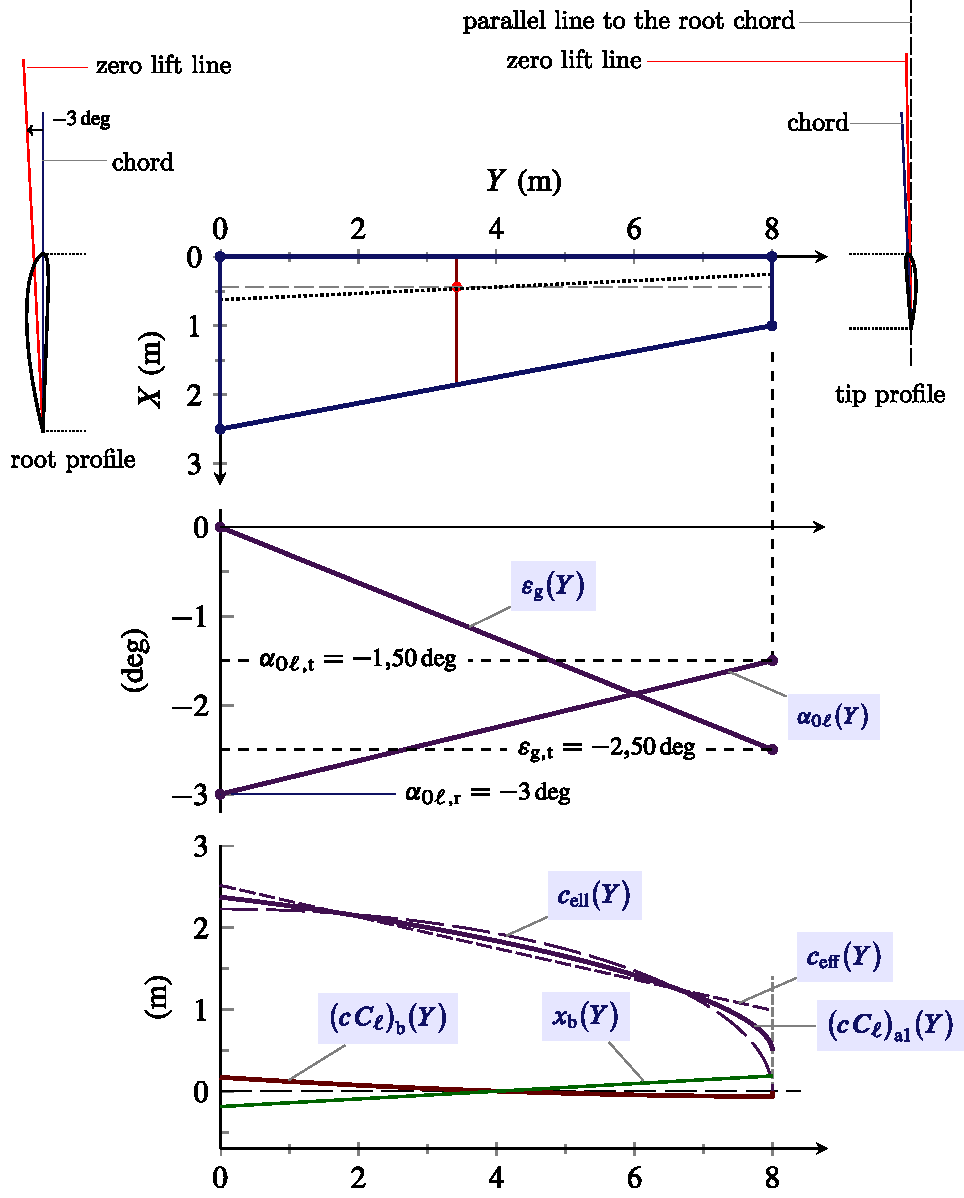
\includegraphics[width=0.90\textwidth]{exercises/wing_Cmac_1/wing_Cmac_1_loading_drawing.pdf}%
%  \caption{\finalhyphendemerits=1000
%           Ala assegnata nell'esempio~\ref{example:Wing:Cmac:A}.
%           Diagrammi del carico addizionale $(cC_\ell)_\mathrm{a1}$, 
%           del carico basico $(cC_\ell)_\mathrm{b}$
%           e del braccio $x_\mathrm{b}(Y)$.}
%  \label{fig:Wing:Cmac:Results:A}%
%\end%
%    %{figure}%
%    {SCfigure}%
%
%\EnlargedFigure% needs two latex passes
%    {t}% #1: t, b, p
%    {images/airfoil_geometry}% #2: the image file included by \includegraphics
%    {width=1.0\textwidth}% #3: option list to pass to \includegraphics, e.g. width=\linewidth,rotate=0
%    {\finalhyphendemerits=1000
%      Alcune caratteristiche geometriche di un profilo alare.}% #4: the caption text
%    {fig:Aero:Profilo:Geometria}% #5: the label
\EnlargedFigureX% needs two latex passes
  {p}% #1: t, b, p
  {%
    \makebox[\textwidth][c]{%
      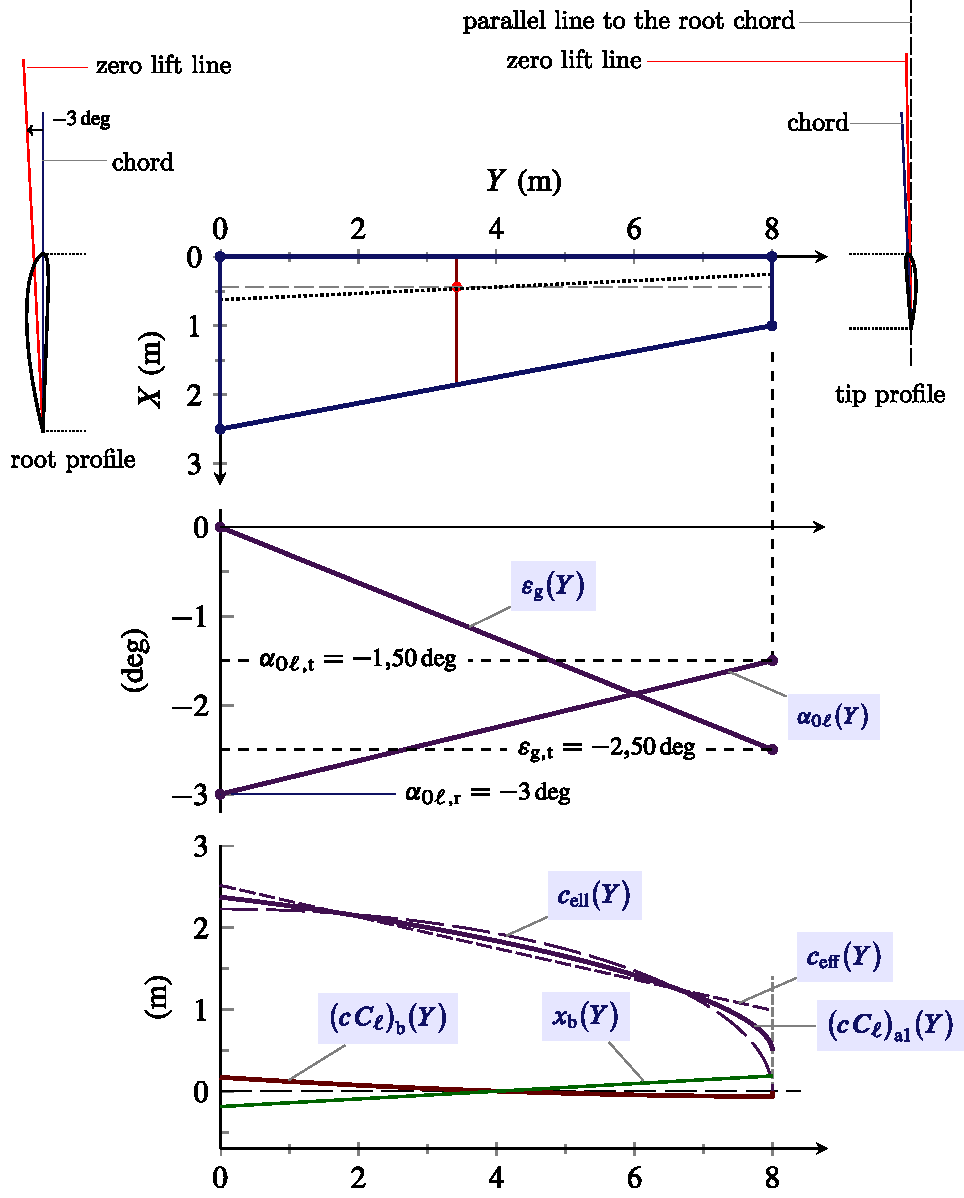
\includegraphics[width=0.90\textwidth]{exercises/wing_Cmac_1/wing_Cmac_1_loading_drawing.pdf}%
    }% end-of-makebox
    \vspace{0.3cm}
  }% #2: the image file included by \includegraphics
  {\finalhyphendemerits=1000
    Ala assegnata nell'esempio~\ref{example:Wing:Cmac:A}.
    Legge dello svergolamento geometrico $\epsilon_\mathrm{g}(y)$ e dello svergolamento
    aerodinamico $\alpha_{0\ell}(Y)$.
    Diagrammi del carico addizionale $(cC_\ell)_\mathrm{a1}$, 
    del carico basico $(cC_\ell)_\mathrm{b}$ e del braccio $x_\mathrm{b}(Y)$.%
  }% #3: the caption text
  {fig:Wing:Cmac:Results:A}%% #4: the label
%
%-----------------------------------------------------------------------------------------------

%=BEGING-EX==================================================================================================
%
\def\mySpanWingMT{10.600000}
\def\mySpanWingIMT{6.360000}
\def\mySpanWingIIMT{4.240000}
\def\myChordRootWingMT{1.440000}
\def\myChordRootWingIMT{1.440000}
\def\myChordRootWingIIMT{1.440000}
\def\myChordTipWingMT{0.860000}
\def\myChordTipWingIMT{1.440000}
\def\myChordTipWingIIMT{0.860000}
\def\mySweepLEWingIIDEG{0.000000}
\def\myCoeffAChordWingI{0.000000}
\def\myCoeffBChordWingIMT{1.440000}
\def\myCoeffAChordWingII{-0.273585}
\def\myCoeffBChordWingIIMT{1.440000}
\def\myAlphaZeroLiftRootWingIDEG{-2.500000}
\def\myAlphaZeroLiftTipWingIDEG{-2.500000}
\def\myAlphaZeroLiftRootWingIRAD{-0.043633}
\def\myAlphaZeroLiftTipWingIRAD{-0.043633}
\def\myAlphaZeroLiftRootWingIIDEG{-2.500000}
\def\myAlphaZeroLiftTipWingIIDEG{-1.000000}
\def\myAlphaZeroLiftRootWingIIRAD{-0.043633}
\def\myAlphaZeroLiftTipWingIIRAD{-0.017453}
\def\myTaperRatioWingI{1.000000}
\def\myTaperRatioWingII{0.597222}
\def\myTwistWingIDEG{0.000000}
\def\myTwistWingIRAD{0.000000}
\def\myTwistWingIIDEG{-3.000000}
\def\myTwistWingIIRAD{-0.052360}
\def\myAreaWingIMTsquared{9.158400}
\def\myAreaWingIIMTsquared{4.876000}
\def\myAreaWingMTsquared{14.034400}
\def\myCoeffAAeroTwistWingIRADMT{0.000000}
\def\myCoeffBAeroTwistWingIRAD{-0.043633}
\def\myCoeffAAeroTwistWingIIRADMT{0.012349}
\def\myCoeffBAeroTwistWingIIRAD{-0.043633}
\def\myCoeffATwistWingIRADMT{0.000000}
\def\myCoeffATwistWingIIRADMT{-0.024698}
\def\myCoeffBTwistWingIRAD{0.000000}
\def\myCoeffBTwistWingIIRAD{0.000000}
\def\myAlphaZeroLiftWingIRAD{-0.028653}
\def\myAlphaZeroLiftWingIDEG{-1.641680}
\def\myAlphaZeroLiftWingIIRAD{0.008329}
\def\myAlphaZeroLiftWingIIDEG{0.477233}
\def\myAlphaZeroLiftWingRAD{-0.020323}
\def\myAlphaZeroLiftWingDEG{-1.164447}

%
\begin{myExerciseX}{Momento di beccheggio intorno al centro aerodinamico dell'ala}{\ding{46}}% \ \Keyboard\ %
\label{exercise:Wing:Cmac:A}

\noindent
Un'ala finita ha le stesse caratteristiche di quella definita nell'esempio~\ref{example:Wing:Cmac:A}
fatta eccezione per la linea dei fuochi, che in questo caso è parallela all'asse $Y$, cioè è
$\Lambda_{c/4}=\SI[round-precision=0]{\mySweepQuarterChordWingDEG}{\degree}$.
La figura~\ref{fig:Wing:Cmac:Results:AA} ne riporta la vista in pianta.

Disegnare la forma in pianta, calcolare la posizione 
$X_{\mathrm{ac}}$ del suo centro aerodinamico
e fornire il valore del \smash{$C_{\mathcal{M}_\mathlarger{\mathrm{ac}}}$} corrispondente.

Verificare che dalle figure~\ref{fig:Wing:Ac:K:One:Plots}, \ref{fig:Wing:Ac:K:Two:Plots}
e~\ref{fig:Wing:Ac:X:AC:From:Apex:Plots} si ottengono i valori:
\[
K_1
  = \mathunderline{mydarkblue}{ \SI[round-precision=3]{\myKOneACDatcomWing}{} }
\;,\quad
K_2 
  = \mathunderline{mydarkblue}{ \SI[round-precision=3]{\myKTwoACDatcomWing}{} }
\;,\quad
\frac{X'_{\mathrm{ac}}}{c_\mathrm{r}}
  = \mathunderline{mydarkblue}{ \SI[round-precision=3]{\myXACOverChordRootDatcomWing}{} }
\]

Tracciare la funzione $x_\mathrm{b}(Y)$ e giustificare la coincidenza
di \smash{$C_{\mathcal{M}_\mathlarger{\mathrm{ac}}}$}
con il momento delle coppie pure di profilo \smash{$C_{\mathcal{M}_\mathlarger{\mathrm{ac,a}}}$}.

\end{myExerciseX}
%=END-EX====================================================================================================

%-----------------------------------------------------------------------------------------------
%\begin%
%  %{figure}
%  {SCfigure}[1.9]%
%  [t]%[H]%[!htbp]
%  %\centering
%  %\checkoddpage
%  %\centering
%    \includegraphics[width=0.90\textwidth]{exercises/wing_Cmac_1/wing_Cmac_1_loading_drawing.pdf}%
%  \caption{\finalhyphendemerits=1000
%           Ala assegnata nell'esempio~\ref{example:Wing:Cmac:A}.
%           Diagrammi del carico addizionale $(cC_\ell)_\mathrm{a1}$, 
%           del carico basico $(cC_\ell)_\mathrm{b}$
%           e del braccio $x_\mathrm{b}(Y)$.}
%  \label{fig:Wing:Cmac:Results:A}%
%\end%
%    %{figure}%
%    {SCfigure}%
%
%\EnlargedFigure% needs two latex passes
%    {t}% #1: t, b, p
%    {images/airfoil_geometry}% #2: the image file included by \includegraphics
%    {width=1.0\textwidth}% #3: option list to pass to \includegraphics, e.g. width=\linewidth,rotate=0
%    {\finalhyphendemerits=1000
%      Alcune caratteristiche geometriche di un profilo alare.}% #4: the caption text
%    {fig:Aero:Profilo:Geometria}% #5: the label
\EnlargedFigureX% needs two latex passes
  {t}% #1: t, b, p
  {%
    \makebox[\textwidth][c]{%
      \includegraphics[width=0.80\textwidth]{exercises/wing_Cmac_1a/wing_Cmac_1a_loading_drawing.pdf}%
    }% end-of-makebox
    \vspace{0.3cm}
  }% #2: the image file included by \includegraphics
  {\finalhyphendemerits=1000
    Ala assegnata nell'esercizio~\ref{exercise:Wing:Cmac:A}.
    Il centro aerodinamico è molto vicino alla linea dei fuochi. Quest'ultima
    è parallela all'asse delle $Y$. L'ingrandimento sulla sinistra mostra che
    il punto di coordinate $(\frac{1}{4}c_\mathrm{r},0)$ è più arretrato del punto
    $(X_{\mathrm{le},\bar{c}}+x_\mathrm{ac},0)$.
  }% #3: the caption text
  {fig:Wing:Cmac:Results:AA}%% #4: the label
%
%-----------------------------------------------------------------------------------------------


%=BEGING-ES===========================================================================================
%
\def\mySpanWingMT{10.600000}
\def\mySpanWingIMT{6.360000}
\def\mySpanWingIIMT{4.240000}
\def\myChordRootWingMT{1.440000}
\def\myChordRootWingIMT{1.440000}
\def\myChordRootWingIIMT{1.440000}
\def\myChordTipWingMT{0.860000}
\def\myChordTipWingIMT{1.440000}
\def\myChordTipWingIIMT{0.860000}
\def\mySweepLEWingIIDEG{0.000000}
\def\myCoeffAChordWingI{0.000000}
\def\myCoeffBChordWingIMT{1.440000}
\def\myCoeffAChordWingII{-0.273585}
\def\myCoeffBChordWingIIMT{1.440000}
\def\myAlphaZeroLiftRootWingIDEG{-2.500000}
\def\myAlphaZeroLiftTipWingIDEG{-2.500000}
\def\myAlphaZeroLiftRootWingIRAD{-0.043633}
\def\myAlphaZeroLiftTipWingIRAD{-0.043633}
\def\myAlphaZeroLiftRootWingIIDEG{-2.500000}
\def\myAlphaZeroLiftTipWingIIDEG{-1.000000}
\def\myAlphaZeroLiftRootWingIIRAD{-0.043633}
\def\myAlphaZeroLiftTipWingIIRAD{-0.017453}
\def\myTaperRatioWingI{1.000000}
\def\myTaperRatioWingII{0.597222}
\def\myTwistWingIDEG{0.000000}
\def\myTwistWingIRAD{0.000000}
\def\myTwistWingIIDEG{-3.000000}
\def\myTwistWingIIRAD{-0.052360}
\def\myAreaWingIMTsquared{9.158400}
\def\myAreaWingIIMTsquared{4.876000}
\def\myAreaWingMTsquared{14.034400}
\def\myCoeffAAeroTwistWingIRADMT{0.000000}
\def\myCoeffBAeroTwistWingIRAD{-0.043633}
\def\myCoeffAAeroTwistWingIIRADMT{0.012349}
\def\myCoeffBAeroTwistWingIIRAD{-0.043633}
\def\myCoeffATwistWingIRADMT{0.000000}
\def\myCoeffATwistWingIIRADMT{-0.024698}
\def\myCoeffBTwistWingIRAD{0.000000}
\def\myCoeffBTwistWingIIRAD{0.000000}
\def\myAlphaZeroLiftWingIRAD{-0.028653}
\def\myAlphaZeroLiftWingIDEG{-1.641680}
\def\myAlphaZeroLiftWingIIRAD{0.008329}
\def\myAlphaZeroLiftWingIIDEG{0.477233}
\def\myAlphaZeroLiftWingRAD{-0.020323}
\def\myAlphaZeroLiftWingDEG{-1.164447}

%
\begin{myExampleX}{Momento di beccheggio intorno al centro aerodinamico dell'ala}{\ding{46}}% \ \Keyboard\ %
\label{example:Wing:Cmac:B}
%
\noindent
L'esempio~\ref{example:Wing:Cmac:A} (si veda la figura~\ref{fig:Wing:Cmac:Results:A}) è ripreso qui considerando 
una legge più accurata del carico basico.
Essa è stata ottenuta numericamente ed è diagrammata nella figura~\ref{fig:Wing:Cmac:Results:BA}.
I valori numerici sono riportati nella tabella~\ref{tab:Wing:Cmac:Results:B}.

Nella figura~\ref{fig:Wing:Cmac:Results:BB} si mette a confronto la funzione
$(cC_\ell)_\mathrm{b,Schrenk}(Y)$, ottenuta in concomitanza dell'applicazione del metodo ingegneristico di 
Schrenk per il carico addizionale (si veda l'esempio~\ref{example:Wing:Cmac:A}),
con la funzione $(cC_\ell)_\mathrm{b}(Y)$, che interpola una sequenza di valori discreti
ottenuti applicando la Teoria della linea portante di Prandtl

\begin{table}[tb]
\caption{%
  Ala assegnata negli esempi~\ref{example:Wing:Cmac:A} e ~\ref{example:Wing:Cmac:B}.
  Valori numerici con cui è stato calcolato il carico basico $(cC_\ell)_\mathrm{b}$ 
  con la Teoria della linea portante.
}
\label{tab:Wing:Cmac:Results:B}
\centering
\includegraphics[width=0.95\textwidth]{exercises/wing_Cmac_2/wing_Cmac_2_loading_table.pdf}
\end{table}

Nel caso qui discusso sia la funzione $x_\mathrm{b}(Y)$ che il valore
di $C_{\mathcal{M}_\mathlarger{\mathrm{ac,b}}}$ coincidono con quanto ricavato
nell'esempio~\ref{example:Wing:Cmac:A}.
Per quanto riguarda il valore di $C_{\mathcal{M}_\mathlarger{\mathrm{ac,b}}}$, disponendo
di un andamento più accurato del carico basico, si ottiene un valore differente

\[
C_{\mathcal{M}_\mathlarger{\mathrm{ac,b}}} 
  =
  \frac{2}{S\,\bar{c}} \int_0^{b/2} \big(cC_{\ell}\big)_\mathrm{b}(Y) \; x_\mathrm{b}(Y)\, \diff{Y}
  = 
  \mathunderline{mydarkblue}{ \SI[round-precision=5]{\myCmZeroBWing}{} }
\]
L'integrale in questa formula è stato valutato numericamente dopo aver definito una funzione
interpolante $(cC_\ell)_\mathrm{b}(Y)$ lineare a tratti nell'intervallo
$[0,\frac{1}{2}b]$.
La figura~\ref{fig:Wing:Cmac:Results:BC} riporta in grafico i valori discreti della
funzione integranda 
%$\big(cC_{\ell}\big)_\mathrm{b}(Y) \, x_\mathrm{b}(Y)$,
$\big(cC_{\ell}\big)_\mathrm{b} \, x_\mathrm{b}$,
già elencati nella settima colonna della tabella~\ref{tab:Wing:Cmac:Results:B}.
L'area sottesa dal grafico della funzione è negativa così come è negativo, ovviamente, il segno
di \smash{$C_{\mathcal{M}_\mathlarger{\mathrm{ac,b}}}$}.

\end{myExampleX}

%=END-ES=====================================================================================================

%-----------------------------------------------------------------------------------------------
\begin%
  %{figure}
  {SCfigure}[1.9]%
  [t]%[H]%[!htbp]
  %\centering
  %\checkoddpage
  %\centering
    \includegraphics[width=0.80\textwidth]{exercises/wing_Cmac_2/wing_Cmac_2_loading_drawing.pdf}%
  \caption{\finalhyphendemerits=1000
           Ala assegnata negli esempi~\ref{example:Wing:Cmac:A} e ~\ref{example:Wing:Cmac:B}.
           Diagrammi del carico addizionale $(cC_\ell)_\mathrm{a1}$ e 
           del carico basico $(cC_\ell)_\mathrm{b}$ ottenuti numericamente
           (dalla Teoria della linea portante)
           e legge $x_\mathrm{b}(Y)$ dei bracci del carico basico.}
  \label{fig:Wing:Cmac:Results:BA}%
\end%
    %{figure}%
    {SCfigure}%
%
%\EnlargedFigure% needs two latex passes
%    {t}% #1: t, b, p
%    {images/airfoil_geometry}% #2: the image file included by \includegraphics
%    {width=1.0\textwidth}% #3: option list to pass to \includegraphics, e.g. width=\linewidth,rotate=0
%    {\finalhyphendemerits=1000
%      Alcune caratteristiche geometriche di un profilo alare.}% #4: the caption text
%    {fig:Aero:Profilo:Geometria}% #5: the label
%\EnlargedFigureX% needs two latex passes
%  {p}% #1: t, b, p
%  {%
%    \makebox[\textwidth][c]{%
%      \includegraphics[width=0.90\textwidth]{exercises/wing_Cmac_1/wing_Cmac_1_loading_drawing.pdf}%
%    }% end-of-makebox
%    \vspace{0.3cm}
%  }% #2: the image file included by \includegraphics
%  {\finalhyphendemerits=1000
%    Ala assegnata nell'esempio~\ref{example:Wing:Cmac:A}.
%    Legge dello svergolamento geometrico $\epsilon_\mathrm{g}(y)$ e dello svergolamento
%    aerodinamico $\alpha_{0\ell}(Y)$.
%    Diagrammi del carico addizionale $(cC_\ell)_\mathrm{a1}$, 
%    del carico basico $(cC_\ell)_\mathrm{b}$ e del braccio $x_\mathrm{b}(Y)$.%
%  }% #3: the caption text
%  {fig:Wing:Cmac:Results:A}%% #4: the label
%
%-----------------------------------------------------------------------------------------------

%-----------------------------------------------------------------------------------------------
\begin%
  %{figure}
  {SCfigure}[1.9]%
  [t]%[H]%[!htbp]
  %\centering
  %\checkoddpage
  %\centering
    \includegraphics[width=0.80\textwidth]{exercises/wing_Cmac_2/wing_Cmac_2_loading_drawing_2.pdf}%
  \caption{\finalhyphendemerits=1000
           Ala assegnata negli esempi~\ref{example:Wing:Cmac:A} e ~\ref{example:Wing:Cmac:B}.
           Dettaglio della figura~\ref{fig:Wing:Cmac:Results:BA}.
           Diagramma del carico basico $(cC_\ell)_\mathrm{b}$ ottenuto numericamente
           con la Teoria della linea portante
           e del carico basico approssimato $(cC_\ell)_\mathrm{b,Schrenk}$ ottenuto in concomitanza
           dell'applicazione del metodo ingegneristico di Schrenk per il carico addizionale
           (si veda anche la figura~\ref{fig:Wing:Cmac:Results:A}).}
  \label{fig:Wing:Cmac:Results:BB}%
\end%
    %{figure}%
    {SCfigure}%
%
%\EnlargedFigure% needs two latex passes
%    {t}% #1: t, b, p
%    {images/airfoil_geometry}% #2: the image file included by \includegraphics
%    {width=1.0\textwidth}% #3: option list to pass to \includegraphics, e.g. width=\linewidth,rotate=0
%    {\finalhyphendemerits=1000
%      Alcune caratteristiche geometriche di un profilo alare.}% #4: the caption text
%    {fig:Aero:Profilo:Geometria}% #5: the label
%\EnlargedFigureX% needs two latex passes
%  {p}% #1: t, b, p
%  {%
%    \makebox[\textwidth][c]{%
%      \includegraphics[width=0.90\textwidth]{exercises/wing_Cmac_1/wing_Cmac_1_loading_drawing.pdf}%
%    }% end-of-makebox
%    \vspace{0.3cm}
%  }% #2: the image file included by \includegraphics
%  {\finalhyphendemerits=1000
%    Ala assegnata nell'esempio~\ref{example:Wing:Cmac:A}.
%    Legge dello svergolamento geometrico $\epsilon_\mathrm{g}(y)$ e dello svergolamento
%    aerodinamico $\alpha_{0\ell}(Y)$.
%    Diagrammi del carico addizionale $(cC_\ell)_\mathrm{a1}$, 
%    del carico basico $(cC_\ell)_\mathrm{b}$ e del braccio $x_\mathrm{b}(Y)$.%
%  }% #3: the caption text
%  {fig:Wing:Cmac:Results:A}%% #4: the label
%
%-----------------------------------------------------------------------------------------------

%-----------------------------------------------------------------------------------------------
\begin%
  %{figure}
  {SCfigure}[1.9]%
  [t]%[H]%[!htbp]
  %\centering
  %\checkoddpage
  %\centering
    \includegraphics[width=0.80\textwidth]{exercises/wing_Cmac_2/wing_Cmac_2_loading_drawing_3.pdf}%
  \caption{\finalhyphendemerits=1000
           Ala assegnata negli esempi~\ref{example:Wing:Cmac:A} e ~\ref{example:Wing:Cmac:B}.
           Diagramma delle due funzioni prodotto $(cC_\ell)_\mathrm{b}(Y)\,x_\mathrm{b}(Y)$ 
           e $(cC_\ell)_\mathrm{b,Schrenk}(Y)\,x_\mathrm{b}(Y)$
           (si veda la figura~\ref{fig:Wing:Cmac:Results:BC}).
           L'integrale di queste funzioni permette di stimare il contributo
           \smash{$C_{\mathcal{M}_\mathlarger{\mathrm{ac,b}}}$} al coefficiente
           di momento di beccheggio \smash{$C_{\mathcal{M}_\mathlarger{\mathrm{ac}}}$}
           dell'ala intorno al suo centro aerodinamico.
  }
  \label{fig:Wing:Cmac:Results:BC}%
\end%
    %{figure}%
    {SCfigure}%
%
%\EnlargedFigure% needs two latex passes
%    {t}% #1: t, b, p
%    {images/airfoil_geometry}% #2: the image file included by \includegraphics
%    {width=1.0\textwidth}% #3: option list to pass to \includegraphics, e.g. width=\linewidth,rotate=0
%    {\finalhyphendemerits=1000
%      Alcune caratteristiche geometriche di un profilo alare.}% #4: the caption text
%    {fig:Aero:Profilo:Geometria}% #5: the label
%\EnlargedFigureX% needs two latex passes
%  {p}% #1: t, b, p
%  {%
%    \makebox[\textwidth][c]{%
%      \includegraphics[width=0.90\textwidth]{exercises/wing_Cmac_1/wing_Cmac_1_loading_drawing.pdf}%
%    }% end-of-makebox
%    \vspace{0.3cm}
%  }% #2: the image file included by \includegraphics
%  {\finalhyphendemerits=1000
%    Ala assegnata nell'esempio~\ref{example:Wing:Cmac:A}.
%    Legge dello svergolamento geometrico $\epsilon_\mathrm{g}(y)$ e dello svergolamento
%    aerodinamico $\alpha_{0\ell}(Y)$.
%    Diagrammi del carico addizionale $(cC_\ell)_\mathrm{a1}$, 
%    del carico basico $(cC_\ell)_\mathrm{b}$ e del braccio $x_\mathrm{b}(Y)$.%
%  }% #3: the caption text
%  {fig:Wing:Cmac:Results:A}%% #4: the label
%
%-----------------------------------------------------------------------------------------------

\setcounter{chapter}{4}
\chapter%
  [Aerodinamica delle fusoliere]%
  {Aerodinamica delle fusoliere}

%=BEGING-ES==================================================================================================
%
\def\myDummyValue{-999}
\def\myMach{0.65}
\def\myDummyValue{-999}
\def\myAreaWingMTsquared{499.17}
\def\myAreaWingFTsquared{5373.01}
\def\mySpanWingMT{59.7408}
\def\mySpanWingFT{196}
\def\myTaperRatioWing{0.305}
\def\myInducedDragFactorWing{0.9}
\def\myIncidenceWingRAD{0.03491}
\def\myIncidenceWingDEG{2}
\def\mySweepLEWingRAD{0.7330383}
\def\mySweepLEWingDEG{42}
\def\myXsiTmaxWing{0.3}
\def\mySweepTmaxWingRAD{0.6814218}
\def\mySweepTmaxWingDEG{39.04259}
\def\myDihedralWingRAD{0.08727}
\def\myDihedralWingDEG{5}
\def\myAlphaZeroLiftMeanWingRAD{-0.03743}
\def\myAlphaZeroLiftMeanWingDEG{-2.1}
\def\myThicknessOverChordMeanWing{0.12}
\def\myCmZeroMeanWing{-0.0737588}
\def\myCLAlphaMeanWingRAD{6.06584}
\def\myCLAlphaMeanWingDEG{0.10587}
\def\myChordRootWingMT{14.69}
\def\myChordRootWingFT{48.2}
\def\myChordTipWingMT{4.48}
\def\myChordTipWingFT{14.7}
\def\myRootChordWingLongitudinalPlaneMT{12.23}
\def\myRootChordWingLongitudinalPlaneFT{40.13}
\def\myXEquivalentChordLEToApexWingMT{0}
\def\myXEquivalentChordLEToApexWingFT{0}
\def\myXEquivalentChordTEToApexWingMT{12.231}
\def\myXEquivalentChordTEToApexWingFT{40.127}
\def\myEquivalentTaperRatioWing{0.366}
\def\myEquivalentSweepLEWingRAD{0.73304}
\def\myEquivalentSweepLEWingDEG{42}
\def\myEquivalentSweepQuarterChordWingRAD{0.69604}
\def\myEquivalentSweepQuarterChordWingDEG{39.88}
\def\myEquivalentSweepHalfChordWingRAD{0.6566}
\def\myEquivalentSweepHalfChordWingDEG{37.621}
\def\myEquivalentSweepTEWingRAD{0.56999}
\def\myEquivalentSweepTEWingDEG{32.658}
\def\myAspectRatioEquivalentWing{7.15}
\def\myAspectRatioWing{7.15}
\def\myMACWingMT{9.29}
\def\myMACWingFT{30.47}
\def\myXMACLEToApexWingMT{8.25}
\def\myXMACLEToApexWingFT{27.06}
\def\myAlphaZeroLiftWingRAD{-0.025009}
\def\myAlphaZeroLiftWingDEG{-1.433}
\def\myCriticalMachNumberMACWing{0.988}
\def\myCLAlphaAtMACWingRAD{6.08087}
\def\myCLAlphaAtMACWingDEG{0.1061313}
\def\myCLAlphaWingRAD{5.72254}
\def\myCLAlphaWingDEG{0.0998771}
\def\myKPolhamus{100}
\def\myCLAlphaPolhamusWingRAD{4.54711}
\def\myCLAlphaPolhamusWingDEG{0.0793621}
\def\myCmZeroAWing{-0.0737588}
\def\myCmZeroBWing{0.0532358}
\def\myCmZeroWing{-0.02052}
\def\myXMACLEToApexWingMT{8.24866}
\def\myXMACLEToApexWingFT{27.06254}
\def\myXsiACWing{0.53693}
\def\myXACOverChordRootDatcomWing{0.900896}
\def\myRiggingAngleWingRAD{0.03490659}
\def\myRiggingAngleWingDEG{2}
\def\myAreaWingIMTsquared{233.45}
\def\myAreaWingIFTsquared{2512.84}
\def\mySpanWingIMT{19.8423}
\def\mySpanWingIFT{65.0994}
\def\myTaperRatioWingI{0.602}
\def\myAspectRatioWingI{1.687}
\def\myMACWingIMT{12.008}
\def\myMACWingIFT{39.396}
\def\mySweepLEWingIRAD{0.73304}
\def\mySweepLEWingIDEG{42}
\def\mySweepTEWingIRAD{0.3011}
\def\mySweepTEWingIDEG{17.251}
\def\myTwistWingIRAD{0}
\def\myTwistWingIDEG{0}
\def\myAlphaZeroLiftRootWingIRAD{-0.04363}
\def\myAlphaZeroLiftRootWingIDEG{-2.5}
\def\myAlphaZeroLiftTipWingIRAD{-0.04363}
\def\myAlphaZeroLiftTipWingIDEG{-2.5}
\def\myAlphaZeroLiftMeanWingIRAD{-0.04363}
\def\myAlphaZeroLiftMeanWingIDEG{-2.5}
\def\myAlphaZeroLiftWingIRAD{-0.02041}
\def\myAlphaZeroLiftWingIDEG{-1.17}
\def\myThicknessOverChordRootWingI{0.15}
\def\myThicknessOverChordTipWingI{0.12}
\def\myThicknessOverChordMeanWingI{0.136}
\def\myCmZeroRootWingI{-0.08}
\def\myCmZeroTipWingI{-0.08}
\def\myCmZeroMeanWingI{-0.08}
\def\myCLAlphaRootWingIRAD{6.15}
\def\myCLAlphaRootWingIDEG{0.1073377}
\def\myCLAlphaTipWingIRAD{6.05}
\def\myCLAlphaTipWingIDEG{0.1055924}
\def\myCLAlphaMeanWingIRAD{6.1041451}
\def\myCLAlphaMeanWingIDEG{0.1065374}
\def\myCLAlphaAtMACWingIRAD{6.1041451}
\def\myCLAlphaAtMACWingIDEG{0.1065374}
\def\myKPolhamusI{100}
\def\myCLAlphaPolhamusWingIRAD{2.25978}
\def\myCLAlphaPolhamusWingIDEG{0.0394407}
\def\myChordRootWingIMT{14.69}
\def\myChordRootWingIFT{48.2}
\def\myChordTipWingIMT{8.84}
\def\myChordTipWingIFT{29}
\def\myXsiacRootWingI{0.25}
\def\myXsiacTipWingI{0.25}
\def\myCriticalMachNumberRootWingI{0.65}
\def\myCriticalMachNumberTipWingI{0.7}
\def\myXMACLEToApexWingIMT{4.096}
\def\myXMACLEToApexWingIFT{13.439}
\def\myYMACWingIMT{4.549}
\def\myYMACWingIFT{14.926}
\def\myXsiACWingI{0.55486}
\def\myKOneACDatcomWingI{1.220232}
\def\myKTwoACDatcomWingI{0.0075}
\def\myXACOverChordRootDatcomWingI{0.462221}
\def\myCoeffATwistWingIRADMT{0}
\def\myCoeffATwistWingIDEGMT{0}
\def\myCoeffATwistWingIRADFT{0}
\def\myCoeffATwistWingIDEGFT{0}
\def\myCoeffBTwistWingIRAD{0}
\def\myCoeffBTwistWingIDEG{0}
\def\myCoeffAChordWingI{-0.58987}
\def\myCoeffBChordWingIMT{14.69136}
\def\myCoeffBChordWingIFT{48.2}
\def\myCoeffAAeroTwistWingIRADMT{0}
\def\myCoeffAAeroTwistWingIDEGMT{0}
\def\myCoeffAAeroTwistWingIRADFT{0}
\def\myCoeffAAeroTwistWingIDEGFT{0}
\def\myCoeffBAeroTwistWingIRAD{-0.04363}
\def\myCoeffBAeroTwistWingIDEG{-2.5}
\def\myCoeffAPercThicknessWingIMT{-0.003024}
\def\myCoeffAPercThicknessWingIFT{-0.000922}
\def\myCoeffBPercThicknessWingI{0.15}
\def\myCoeffAClalphaWingIRADMT{-0.0100795}
\def\myCoeffAClalphaWingIRADFT{-0.0030722}
\def\myCoeffAClalphaWingIDEGMT{-0.0001759}
\def\myCoeffAClalphaWingIDEGFT{-5.36e-05}
\def\myCoeffBClalphaWingIRAD{6.15}
\def\myCoeffBClalphaWingIDEG{352.369}
\def\myCoeffACmZeroWingIMT{0}
\def\myCoeffACmZeroWingIFT{0}
\def\myCoeffBCmZeroWingI{-0.08}
\def\myCoeffAXsiACWingIMT{0}
\def\myCoeffAXsiACWingIFT{0}
\def\myCoeffBXsiACWingI{0.25}
\def\myCoeffAMachCrWingIMT{0.00504}
\def\myCoeffAMachCrWingIFT{0.001536}
\def\myCoeffBMachCrWingI{0.7}
\def\myAreaWingIIMTsquared{265.72}
\def\myAreaWingIIFTsquared{2860.18}
\def\myAreaWingIIPrimeMTsquared{358.79}
\def\myAreaWingIIPrimeFTsquared{3861.99}
\def\mySpanWingIIMT{39.8985}
\def\mySpanWingIIFT{130.9006}
\def\mySpanWingIIPrimeMT{49.81965}
\def\mySpanWingIIPrimeFT{163.4503}
\def\myAspectRatioWingII{5.991}
\def\myAspectRatioWingIIPrime{6.918}
\def\myMACWingIIMT{6.898}
\def\myMACWingIIFT{22.63}
\def\myMACWingIIPrimeMT{7.545}
\def\myMACWingIIPrimeFT{24.752}
\def\myTaperRatioWingII{0.507}
\def\myTaperRatioWingIIPrime{0.452}
\def\mySweepLEWingIIRAD{0.73304}
\def\mySweepLEWingIIDEG{42}
\def\mySweepTEWingIIRAD{0.59849}
\def\mySweepTEWingIIDEG{34.291}
\def\myTwistWingIIRAD{-0.05236}
\def\myTwistWingIIDEG{-3}
\def\myAlphaZeroLiftRootWingIIRAD{-0.04363}
\def\myAlphaZeroLiftRootWingIIDEG{-2.5}
\def\myAlphaZeroLiftTipWingIIRAD{-0.01745}
\def\myAlphaZeroLiftTipWingIIDEG{-1}
\def\myAlphaZeroLiftMeanWingIIRAD{-0.03197}
\def\myAlphaZeroLiftMeanWingIIDEG{-1.8}
\def\myAlphaZeroLiftWingIIRAD{-0.0046}
\def\myAlphaZeroLiftWingIIDEG{-0.26}
\def\myThicknessOverChordRootWingII{0.12}
\def\myThicknessOverChordTipWingII{0.09}
\def\myThicknessOverChordMeanWingII{0.107}
\def\myCmZeroRootWingII{-0.08}
\def\myCmZeroTipWingII{-0.04}
\def\myCmZeroMeanWingII{-0.0642127}
\def\myCLAlphaRootWingIIRAD{6.05}
\def\myCLAlphaRootWingIIDEG{0.1055924}
\def\myCLAlphaTipWingIIRAD{6.01}
\def\myCLAlphaTipWingIIDEG{0.1048943}
\def\myCLAlphaMeanWingIIRAD{6.03218}
\def\myCLAlphaMeanWingIIDEG{0.1052814}
\def\myCLAlphaAtMACWingIIRAD{5.9604275}
\def\myCLAlphaAtMACWingIIDEG{0.1040291}
\def\myKPolhamusII{100}
\def\myCLAlphaPolhamusWingIIRAD{4.50859}
\def\myCLAlphaPolhamusWingIIDEG{0.0786898}
\def\myChordRootWingIIMT{8.84}
\def\myChordRootWingIIFT{29}
\def\myChordTipWingIIMT{4.48}
\def\myChordTipWingIIFT{14.7}
\def\myXsiacRootWingII{0.25}
\def\myXsiacTipWingII{0.25}
\def\myCriticalMachNumberRootWingII{0.7}
\def\myCriticalMachNumberTipWingII{0.7}
\def\myXMACLEToApexWingIIMT{8.002}
\def\myXMACLEToApexWingIIFT{26.252}
\def\myYMACWingIIMT{8.887}
\def\myYMACWingIIFT{29.156}
\def\myXsiACWingII{0.11269}
\def\myKOneACDatcomWingII{1.311488}
\def\myKTwoACDatcomWingII{1.008142}
\def\myXACOverChordRootDatcomWingII{1.094066}
\def\myCoeffATwistWingIIRADMT{-0.002625}
\def\myCoeffATwistWingIIDEGMT{-0.15038}
\def\myCoeffATwistWingIIRADFT{-0.0008}
\def\myCoeffATwistWingIIDEGFT{-0.0458363}
\def\myCoeffBTwistWingIIRAD{0}
\def\myCoeffBTwistWingIIDEG{0}
\def\myCoeffAChordWingII{-0.21849}
\def\myCoeffBChordWingIIMT{8.8392}
\def\myCoeffBChordWingIIFT{29}
\def\myCoeffAAeroTwistWingIIRADMT{0.001312}
\def\myCoeffAAeroTwistWingIIDEGMT{0.07519}
\def\myCoeffAAeroTwistWingIIRADFT{0.0004}
\def\myCoeffAAeroTwistWingIIDEGFT{0}
\def\myCoeffBAeroTwistWingIIRAD{-0.04363}
\def\myCoeffBAeroTwistWingIIDEG{-2.5}
\def\myCoeffAPercThicknessWingIIMT{-0.001504}
\def\myCoeffAPercThicknessWingIIFT{-0.000458}
\def\myCoeffBPercThicknessWingII{0.12}
\def\myCoeffAClalphaWingIIRADMT{-0.0020051}
\def\myCoeffAClalphaWingIIRADFT{-0.0006112}
\def\myCoeffAClalphaWingIIDEGMT{-3.5e-05}
\def\myCoeffAClalphaWingIIDEGFT{-1.07e-05}
\def\myCoeffBClalphaWingIIRAD{6.05}
\def\myCoeffBClalphaWingIIDEG{346.639}
\def\myCoeffACmZeroWingIIMT{0.0020051}
\def\myCoeffACmZeroWingIIFT{0.0006112}
\def\myCoeffBCmZeroWingII{-0.08}
\def\myCoeffAXsiACWingIIMT{0}
\def\myCoeffAXsiACWingIIFT{0}
\def\myCoeffBXsiACWingII{0.25}
\def\myCoeffAMachCrWingIIMT{0}
\def\myCoeffAMachCrWingIIFT{0}
\def\myCoeffBMachCrWingII{0.7}
\def\myAreaWingCrankedMTsquared{499.17}
\def\myAreaWingCrankedFTsquared{5373.01}
\def\myMACWingCrankedMT{9.28755}
\def\myMACWingCrankedFT{30.47096}
\def\myAspectRatioWingCranked{7.15}
\def\myXMACLEToApexWingCrankedMT{6.17513}
\def\myXMACLEToApexWingCrankedFT{20.2596}
\def\myXXMACLEToApexWingCrankedMT{8.24866}
\def\myXXMACLEToApexWingCrankedFT{27.06254}
\def\myYMACWingCrankedMT{6.85817}
\def\myYMACWingCrankedFT{22.50056}
\def\myYYMACWingCrankedMT{9.16107}
\def\myYYMACWingCrankedFT{30.05599}

\def\mySpanWingMT{10.600000}
\def\mySpanWingIMT{6.360000}
\def\mySpanWingIIMT{4.240000}
\def\myChordRootWingMT{1.440000}
\def\myChordRootWingIMT{1.440000}
\def\myChordRootWingIIMT{1.440000}
\def\myChordTipWingMT{0.860000}
\def\myChordTipWingIMT{1.440000}
\def\myChordTipWingIIMT{0.860000}
\def\mySweepLEWingIIDEG{0.000000}
\def\myCoeffAChordWingI{0.000000}
\def\myCoeffBChordWingIMT{1.440000}
\def\myCoeffAChordWingII{-0.273585}
\def\myCoeffBChordWingIIMT{1.440000}
\def\myAlphaZeroLiftRootWingIDEG{-2.500000}
\def\myAlphaZeroLiftTipWingIDEG{-2.500000}
\def\myAlphaZeroLiftRootWingIRAD{-0.043633}
\def\myAlphaZeroLiftTipWingIRAD{-0.043633}
\def\myAlphaZeroLiftRootWingIIDEG{-2.500000}
\def\myAlphaZeroLiftTipWingIIDEG{-1.000000}
\def\myAlphaZeroLiftRootWingIIRAD{-0.043633}
\def\myAlphaZeroLiftTipWingIIRAD{-0.017453}
\def\myTaperRatioWingI{1.000000}
\def\myTaperRatioWingII{0.597222}
\def\myTwistWingIDEG{0.000000}
\def\myTwistWingIRAD{0.000000}
\def\myTwistWingIIDEG{-3.000000}
\def\myTwistWingIIRAD{-0.052360}
\def\myAreaWingIMTsquared{9.158400}
\def\myAreaWingIIMTsquared{4.876000}
\def\myAreaWingMTsquared{14.034400}
\def\myCoeffAAeroTwistWingIRADMT{0.000000}
\def\myCoeffBAeroTwistWingIRAD{-0.043633}
\def\myCoeffAAeroTwistWingIIRADMT{0.012349}
\def\myCoeffBAeroTwistWingIIRAD{-0.043633}
\def\myCoeffATwistWingIRADMT{0.000000}
\def\myCoeffATwistWingIIRADMT{-0.024698}
\def\myCoeffBTwistWingIRAD{0.000000}
\def\myCoeffBTwistWingIIRAD{0.000000}
\def\myAlphaZeroLiftWingIRAD{-0.028653}
\def\myAlphaZeroLiftWingIDEG{-1.641680}
\def\myAlphaZeroLiftWingIIRAD{0.008329}
\def\myAlphaZeroLiftWingIIDEG{0.477233}
\def\myAlphaZeroLiftWingRAD{-0.020323}
\def\myAlphaZeroLiftWingDEG{-1.164447}

%
\begin{myExampleX}{Caratteristiche aerodinamiche della fusoliera}{\ding{46}}% \ \Keyboard\ %
\label{example:Fuselage:Multhopp:A}
%
\noindent
Si vogliono calcolare i coefficienti \smash{$C_{\mathcal{M}_\mathlarger{0,\Body}}$}
e \smash{$C_{\mathcal{M}_\mathlarger{\alpha},\Body}$}
di una fusoliera con il metodo di integrazione per strisce
(\emph{Strip Integration Method}) di Multhopp.
A tale scopo si considera una configurazione ala-fusoliera (\emph{Wing-Body})
simile a quella di un Boeing~747.

L'ala accoppiata alla fusoliera è praticamente coincidente con quella 
dell'esercizio~\ref{exercise:Wing:Aerodynamic:Center:Cranked}.
Ecco alcune sue caratteristiche che saranno utilizzate per i calcoli relativi alla fusoliera:
\[
\AR=\SI[round-precision=2]{\myAspectRatioWing}{}\;,
\quad
b=\SI[round-precision=2]{\mySpanWingMT}{m}\;,
\quad
S = \SI[round-precision=1]{\myAreaWingMTsquared}{m^2}\;,
\quad
c_\mathrm{r}=\SI[round-precision=1]{\myChordRootWingMT}{m}\;
\quad
\bar{c} = \SI[round-precision=2]{\myMACWingMT}{m}
\]
\[
\alpha_{0L,\Wing} %= \SI[round-precision=4]{\myAlphaZeroLiftWingRAD}{rad}
  =\SI[round-precision=1]{\myAlphaZeroLiftWingDEG}{deg}\;,
\quad
i_\Wing=\SI[round-precision=1]{\myRiggingAngleWingDEG}{deg}\;,
\quad
\lambda\equiv\lambda_\text{eqv}=\SI[round-precision=2]{\myEquivalentTaperRatioWing}{}\;,
\quad
\Lambda_{c/4}\equiv\Lambda_{c/4,\text{eqv}} = \SI[round-precision=1]{\myEquivalentSweepLEWingDEG}{deg}
\]
Inoltre,
l'ala assegnata ha un gradiente di portanza 
%\[
%\AR 
%  = \frac{b^2}{S}
%  = \frac{
%      \big( \SI[round-precision=1]{\mySpanWingMT}{\metre} \big)^2
%    }{
%      \SI[round-precision=1]{\myAreaWingMTsquared}{\metre^2}
%    }
%  = \mathunderline{mydarkblue}{ \SI[round-precision=2]{\myAspectRatioWing}{} }
%\]
%\[
%C_{L_\mathlarger{\alpha}}
%  = 
%    \frac{
%      \bar{C}_{\ell_\mathlarger{\alpha}}
%    }{
%      1 + \dfrac{\bar{C}_{\ell_\mathlarger{\alpha}}}{\pi \AR \, e_\Wing}
%    }
%  =
%    \frac{
%      \SI[round-precision=3]{\myCLAlphaMeanWingRAD}{\radian^{-1}}
%    }{
%      1 + 
%        \dfrac{ \SI[round-precision=3]{\myCLAlphaMeanWingRAD}{\radian^{-1}} }{
%          \num[round-precision=2]{3.14} 
%          \cdot \SI[round-precision=2]{\myAspectRatioWing}{}
%          \cdot \SI[round-precision=2]{\myInducedDragFactorWing}{}
%        }
%    }
%  = \mathunderline{mydarkblue}{ \SI[round-precision=3]{\myCLAlphaWingRAD}{\radian^{-1}} }
%  = \mathunderline{mydarkblue}{ \SI[round-precision=4]{\myCLAlphaWingDEG}{\deg^{-1}} }
%\]
%avendo assunto uno \emph{span efficiency factor} 
%%$e_\Wing=\SI[round-precision=2]{\myInducedDragFactorWing}{}$.
%dato dalla formula empirica%
%\footnote{%
%  S. A. Brandt, R. J. Stiles, J. J. Bertin,
%  \emph{Introduction to Aeronautics, A design Perspective},
%  AIAA Education Series, 
%  American Institute of Aeronautics and Astronautics, Reston, VA, 2004.
%}
%\[
%e_\Wing = \frac{2}{2-\AR+\sqrt{4+\AR^2\big(1+\tan^2\Lambda_{t_\mathrm{max}}\big)}}
%\]
%con $\Lambda_{t_\mathrm{max}}$ l'angolo di freccia della linea dei punti di spessore percentuale
%massimo dei profili; nel caso considerato tutti gli spessori percentuali si trovano
%al $30\%$ delle corde e 
%$\Lambda_{t_\mathrm{max}} = \SI[round-precision=2]{\mySweepTmaxWingDEG}{\deg}$
%e 
%$\tan \Lambda_{t_\mathrm{max}} = \calcSI[round-precision=3,fixed-exponent=0,scientific-notation=fixed]{tan(\mySweepTmaxWingRAD)}{}$.
%
$C_{L_\mathlarger{\alpha},\Wing}=\SI[round-precision=2]{\myCLAlphaPolhamusWingRAD}{rad^{-1}}=\SI[round-precision=4]{\myCLAlphaPolhamusWingDEG}{deg^{-1}}$.

Per quanto riguarda le condizioni operative di riferimento, in questo esempio si assume un
numero di Mach di volo $M=\SI[round-precision=2]{\myMach}{}$
e una quota di volo $h_\mathrm{ASL}=\SI[round-precision=2]{\myAltitudeMT}{\metre}$.

La vista laterale e la vista dall'alto della fusoliera sono riportate nelle figure~\ref{fig:Fuselage:Multhopp:Results:AA:A} e~\ref{fig:Fuselage:Multhopp:Results:AA:B}.
Detta $X$ la coordinata longitudinale che corre verso poppa lungo 
la retta di riferimento della fusoliera (\emph{Fuselage Reference Line}, FRL),
con origine all'estremità anteriore, e $Z$ la coordinata ad essa normale 
presa nel piano di simmetria, si riconoscono:
\begin{compactitem}[{\color{gray}$\circ$}]% needs paralist package
\item
la funzione $w_\mathrm{f}(X)$, larghezza della vista in pianta della fusoliera alla stazione $X$,
\item
la coppia di funzioni
$\big(X_\mathrm{cl,f}(X),Z_\mathrm{cl,f}(X)\big)$, che descrivono la linea media
(\emph{camber line}) della vista laterale,
\item
la funzione $i_\mathrm{cl,f}(X)$, che rappresenta l'angolo, con segno cambiato, formato
della tangente locale alla linea media con la FRL.
\end{compactitem}

Una discretizzazione per strisce della fusoliera --- rappresentata visivamente nella
figura~\ref{fig:Fuselage:Multhopp:Results:AA} 
con $N_{\mathrm{f}0}=\num[round-precision=0]{\myNoStripCMZeroBody}$ strisce
di spessore $\upDelta X=\SI[round-precision=1]{\myDxStripCMZeroBodyMT}{m}$
---
ha portato ai valori numerici elencati nella tabella~\ref{tab:Fuselage:Multhopp:Results:A:A}.
In essa, per $k=1,\ldots,\num[round-precision=0]{\myNoStripCMZeroBody}$, si osservano le coordinate 
$\big(X_{\mathrm{cl,f}_\mathlarger{k}},Z_{\mathrm{cl,f}_\mathlarger{k}}\big)$ dei centroidi
di ciascuna striscia, le larghezze $w_{\mathrm{f}_\mathlarger{k}}$ 
e gli angoli $i_{\mathrm{cl,f}_\mathlarger{k}}$.

%-----------------------------------------------------------------------------------------------
%\begin%
%  %{figure}
%  {SCfigure}[1.9]%
%  [t]%[H]%[!htbp]
%  %\centering
%  %\checkoddpage
%  %\centering
%    \includegraphics[width=0.90\textwidth]{exercises/wing_Cmac_1/wing_Cmac_1_loading_drawing.pdf}%
%  \caption{\finalhyphendemerits=1000
%           Ala assegnata nell'esempio~\ref{example:Wing:Cmac:A}.
%           Diagrammi del carico addizionale $(cC_\ell)_\mathrm{a1}$, 
%           del carico basico $(cC_\ell)_\mathrm{b}$
%           e del braccio $x_\mathrm{b}(Y)$.}
%  \label{fig:Wing:Cmac:Results:A}%
%\end%
%    %{figure}%
%    {SCfigure}%
%
%\EnlargedFigure% needs two latex passes
%    {t}% #1: t, b, p
%    {images/airfoil_geometry}% #2: the image file included by \includegraphics
%    {width=1.0\textwidth}% #3: option list to pass to \includegraphics, e.g. width=\linewidth,rotate=0
%    {\finalhyphendemerits=1000
%      Alcune caratteristiche geometriche di un profilo alare.}% #4: the caption text
%    {fig:Aero:Profilo:Geometria}% #5: the label
\EnlargedFigureX% needs two latex passes
  {p}% #1: t, b, p
  {%
    \begin{tabular}{@{}c@{}}
    \subfloat[Vista laterale\label{fig:Fuselage:Multhopp:Results:AA:A}]{%
    \makebox[\textwidth][c]{%
      \includegraphics[width=0.90\textwidth]{exercises/fuselage_multhopp_1/fuselage_sideview_1.pdf}%
    }% end-of-makebox
    }% end-of-subfloat
    \\
    \subfloat[Vista dall'alto\label{fig:Fuselage:Multhopp:Results:AA:B}]{%
    \makebox[\textwidth][c]{%
      \rule{2.2mm}{0pt}% --> hack
      \includegraphics[width=0.88\textwidth]{exercises/fuselage_multhopp_1/fuselage_topview_1.pdf}%
    }% end-of-makebox
    }% end-of-subfloat
    \\
    \subfloat[Incidenza della tangente locale alla linea media\label{fig:Fuselage:Multhopp:Results:AA:C}]{%
    \makebox[\textwidth][c]{%
      \rule{3.7mm}{0pt}% --> hack
      \includegraphics[width=0.895\textwidth]{exercises/fuselage_multhopp_1/fuselage_icl.pdf}%
    }% end-of-makebox
    }% end-of-subfloat
    \end{tabular}
    \vspace{0.3cm}
  }% #2: the image file included by \includegraphics
  {\finalhyphendemerits=1000
    Fusoliera di un Boeing~747.
    Discretizzazione della proiezione laterale per il calcolo approssimato del coefficiente
    \smash{$C_{\mathcal{M}0,\Body}$}
    con il metodo di integrazione per strisce di Multhopp.
    In basso l'angolo $i_\mathrm{cl}$ formato dalla tangente locale alla linea media (\emph{camber line})
    della fusoliera con la FRL.
  }% #3: the caption text
  {fig:Fuselage:Multhopp:Results:AA}%% #4: the label
%
%-----------------------------------------------------------------------------------------------

Il coefficiente di momento di beccheggio dovuto alla fusoliera in condizioni di portanza nulla
--- cioè quando è $L_{\Wing\Body}=0$ --- è dato dalla formula
\[
%\begin{equation}\label{eq:Aero:CMBW:Zero}
C_{\mathcal{M}_\mathlarger{0,\Body}} \equiv C_{\mathcal{M}_\mathlarger{0L,\Body(\Wing)}}
    = \frac{\pi}{2}
    \frac{k_2 - k_1}{S \bar{c}}
    %\frac{k_2 - k_1}{\num[round-precision=1]{36.5}\msp S \bar{c}}
      \, \int_{0}^{l_\Body} w_\mathrm{f}^2\msp(X) \,
      \big[\msp i_\Wing -\alpha_{0L,\text{W}} + i_{\mathrm{cl,f\msp}}(X)\msp\big] \diff{X}
%\end{equation}
\]
in cui gli angoli vanno espressi in \si{rad}.
Per valutare il risultato finale --- essendo note le grandezze
$S$, $\bar{c}$, $i_{\Wing}$ e $\alpha_{0L,\Wing}$, relative all'ala ---
si devono determinare le leggi $w_\mathrm{f}\msp(X)$ e $i_{\mathrm{cl,f\msp}}(X)$
e si deve calcolare il coefficiente di massa apparente $k_2-k_1$.
Quest'ultimo si ricava dalla figura~\ref{fig:Fuselage:Munch:Mass:Factor} ottenendo
\[
k_2-k_1=\SI[round-precision=2]{\myFuselageMunchMassFactor}{}
\]
corrispondente al fattore di snellezza della fusoliera
% $\text{\itshape FFR}=l_\Body/d_\Body=\SI[round-precision=2]{\myFuselageFinenessRatio}{}$.
$l_\Body/d_\Body=\SI[round-precision=1]{\myFuselageFinenessRatio}{}$ (\emph{Fuselage Fineness Ratio}, FFR).

La formula di calcolo del \smash{$C_{\mathcal{M}_\mathlarger{0,\Body}}$} viene approssimata sostituendo all'integrale definito
una sommatoria. Quest'approssimazione si basa sulla discretizzazione della forma di fusoliera su menzionata.
Con riferimento ai valori della tabella~\ref{tab:Fuselage:Multhopp:Results:A:A} si ottiene
\[
%\begin{equation}\label{eq:Aero:CMBW:Zero}
C_{\mathcal{M}_\mathlarger{0,\Body}} \approx
    \frac{\pi}{2}
    \frac{k_2 - k_1}{S \bar{c}} \,
    %\frac{k_2 - k_1}{\num[round-precision=1]{36.5}\msp S \bar{c}}
      \sum_{k=1}^{\num[round-precision=0]{\myNoStripCMZeroBody}} 
        w_{\mathrm{f}_\mathlarger{k}}^2
        \Big(\msp i_\Wing -\alpha_{0L,\text{W}} + i_{\mathrm{cl,f}_\mathlarger{k}}\msp\Big) \upDelta X
  = 
    \mathunderline{mydarkblue}{ 
      \SI[round-precision=4]{\myFuselagePitchingMomentCoefficienAtZeroLift}{} 
    }
%\end{equation}
\]

Come si intuisce dalla vista laterale della fusoliera e dall'andamento della linea media
--- si veda il diagramma della sequenza $\big(X_{\mathrm{cl,f}_\mathlarger{k}},i_{\mathrm{cl,f}_\mathlarger{k}}\big)$ 
nella figura~\ref{fig:Fuselage:Multhopp:Results:AA:C} --- 
per una corrente che incide con un angolo
$-i_\Wing+\alpha_{0L,\Wing}=\calcSI[round-precision=1,fixed-exponent=0,scientific-notation=fixed]{-(\myIncidenceWingDEG)+\myAlphaZeroLiftWingDEG}{deg}$
rispetto alla retta di riferimento della fusoliera
il momento di beccheggio è picchiante.

%-----------------------------------------------------------------------------------------------
%
\begin{table}[tb]
\caption{%
  Valori discreti utilizzati nella formule di calcolo del coefficiente di 
  momento \smash{$C_{\mathcal{M}_\mathlarger{0,\Body}}$}.
}
\label{tab:Fuselage:Multhopp:Results:A:A}
\centering
\includegraphics[width=0.38\textwidth]{exercises/fuselage_multhopp_1/fuselage_multhopp_table_1.pdf}
\end{table}
%
%-----------------------------------------------------------------------------------------------

%-----------------------------------------------------------------------------------------------
\begin%
  %{figure}
  {SCfigure}[1.9]%
  [t]%[H]%[!htbp]
  %\centering
  %\checkoddpage
  %\centering
    \includegraphics[width=0.58\textwidth]{exercises/fuselage_multhopp_1/fuselage_k2_minus_k1_res.pdf}%
  \caption{\finalhyphendemerits=1000
           Coefficiente di massa apparente $k_2-k_1$ della fusoliera
           in funzione del fattore di snellezza $l_\Body/d_\Body$ 
           (\emph{Fuselage Fineness Ratio}, FFR).}
  \label{fig:Fuselage:Munch:Mass:Factor}%
\end%
    %{figure}%
    {SCfigure}%
%
%\EnlargedFigure% needs two latex passes
%    {t}% #1: t, b, p
%    {images/airfoil_geometry}% #2: the image file included by \includegraphics
%    {width=1.0\textwidth}% #3: option list to pass to \includegraphics, e.g. width=\linewidth,rotate=0
%    {\finalhyphendemerits=1000
%      Alcune caratteristiche geometriche di un profilo alare.}% #4: the caption text
%    {fig:Aero:Profilo:Geometria}% #5: the label
%\EnlargedFigureX% needs two latex passes
%  {t}% #1: t, b, p
%  {%
%    \begin{tabular}{@{}c@{}}
%    \makebox[\textwidth][c]{%
%      \includegraphics[width=1.00\textwidth]{exercises/fuselage_multhopp_1/fuselage_sideview_1.pdf}%
%    }% end-of-makebox
%    \\
%    \makebox[\textwidth][c]{%
%      \rule{2.2mm}{0pt}% --> hack
%      \includegraphics[width=0.98\textwidth]{exercises/fuselage_multhopp_1/fuselage_topview_1.pdf}%
%    }% end-of-makebox
%    \end{tabular}
%    \vspace{0.3cm}
%  }% #2: the image file included by \includegraphics
%  {\finalhyphendemerits=1000
%    Fusoliera assegnata nell'esempio~\ref{example:Fuselage:Multhopp:A}.
%    Discretizzazione della proiezione laterale per il calcolo approssimato dei coefficienti
%    \smash{$C_{\mathcal{M}0,\Body}$} e \smash{$C_{\mathcal{M}_\mathlarger{\alpha},\Body}$}
%    con il metodo di integrazione per strisce di Multhopp.
%  }% #3: the caption text
%  {fig:Fuselage:Multhopp:Results:AA}%% #4: the label
%
%-----------------------------------------------------------------------------------------------


L'attenzione si sposta ora sul gradiente del coefficiente di momento di beccheggio della fusoliera.
Esso è dato dalla formula
\[
%\begin{equation}\label{eq:Aero:CMBW:Alpha:Multhopp}
C_{\mathcal{M}_\mathlarger{\alpha},\Body} 
  % \equiv \bigg(\frac{\partial \CM}{\partial\alpha}\bigg)_{\!\Body(\Wing)} 
  \equiv \big(C_{\mathcal{M}_\alpha}\big)_{\!\Body(\Wing)} 
  =
    \frac{\pi}{2 S \bar{c}}\, \int_{0}^{l_\Body} w_\mathrm{f}(X)^2 \,
      \bigg(1+\frac{\partial\epsilon_\mathrm{u}(X)}{\partial\alpha}\bigg) \diff{X}
%\end{equation}
\]
dove $\epsilon_\mathrm{u}(X)$ è l'angolo di \emph{upwash} indotto dalla superficie 
portante principale alla generica stazione longitudinale $X$
(si osservi che a valle dell'ala $\epsilon_\mathrm{u}=-\epsilon_\mathrm{u}<0$, dove
cioè il \emph{downwash} $\epsilon >0$). 

Risulta conveniente scomporre l'integrale a secondo membro nella somma di tre integrali.
Essi saranno estesi, rispettivamente, alla parte anteriore della fusoliera
(\emph{forebody}), che va dalla prua al bordo d'attacco della corda di radice
dell'ala, alla parte di fusoliera sottesa dalla radice alare (\emph{wing trunk})
e alla parte posteriore (\emph{afterbody}), che va dal bordo d'uscita della corda di radice
alare fino alla poppa.

%-----------------------------------------------------------------------------------------------
\begin%
  %{figure}
  {SCfigure}[1.9]%
  [t]%[H]%[!htbp]
  %\centering
  %\checkoddpage
  %\centering
    \includegraphics[width=0.88\textwidth]{exercises/fuselage_multhopp_1/fuselage_sideview_1_forebody.pdf}%
  \caption{\finalhyphendemerits=1000
           Vista laterale della parte di fusoliera antistante il bordo d'attacco
           della corda di radice (\emph{forebody}) e discretizzazione in 
           \num[round-precision=0]{\myNoStripForebodyCMAlphaBody} strisce.
           Definizione delle coordinate adimensionali $\tilde{x}_1/c_\mathrm{r}$
           e $x_1/c_\mathrm{r}$ utilizzate nella figura~\ref{fig:Fuselage:Upwash:Gradient}.
  }
  \label{fig:Fuselage:Sideview:Forebody}%
\end%
    %{figure}%
    {SCfigure}%
%
%\EnlargedFigure% needs two latex passes
%    {t}% #1: t, b, p
%    {images/airfoil_geometry}% #2: the image file included by \includegraphics
%    {width=1.0\textwidth}% #3: option list to pass to \includegraphics, e.g. width=\linewidth,rotate=0
%    {\finalhyphendemerits=1000
%      Alcune caratteristiche geometriche di un profilo alare.}% #4: the caption text
%    {fig:Aero:Profilo:Geometria}% #5: the label
%\EnlargedFigureX% needs two latex passes
%  {t}% #1: t, b, p
%  {%
%    \begin{tabular}{@{}c@{}}
%    \makebox[\textwidth][c]{%
%      \includegraphics[width=1.00\textwidth]{exercises/fuselage_multhopp_1/fuselage_sideview_1.pdf}%
%    }% end-of-makebox
%    \\
%    \makebox[\textwidth][c]{%
%      \rule{2.2mm}{0pt}% --> hack
%      \includegraphics[width=0.98\textwidth]{exercises/fuselage_multhopp_1/fuselage_topview_1.pdf}%
%    }% end-of-makebox
%    \end{tabular}
%    \vspace{0.3cm}
%  }% #2: the image file included by \includegraphics
%  {\finalhyphendemerits=1000
%    Fusoliera assegnata nell'esempio~\ref{example:Fuselage:Multhopp:A}.
%    Discretizzazione della proiezione laterale per il calcolo approssimato dei coefficienti
%    \smash{$C_{\mathcal{M}0,\Body}$} e \smash{$C_{\mathcal{M}_\mathlarger{\alpha},\Body}$}
%    con il metodo di integrazione per strisce di Multhopp.
%  }% #3: the caption text
%  {fig:Fuselage:Multhopp:Results:AA}%% #4: the label
%
%-----------------------------------------------------------------------------------------------

Con riferimento alle figure~\ref{fig:Fuselage:Sideview:Forebody} e~\ref{fig:Fuselage:Sideview:Afterbody}
si introducono tre nuove coordinate longitudinali lungo la FRL:
\begin{compactitem}[{\color{gray}$\circ$}]% needs paralist package
\item
la coordinata $x_1$ che corre verso prua e ha origine al bordo
d'attacco della radice alare,
\item
la coordinata $x_\Wing$ che corre verso poppa e ha la stessa origine di $x_1$,
\item
la coordinata $x_2$ che corre verso poppa e ha origine al bordo d'uscita della radice alare.
\end{compactitem}

La formula di calcolo del \smash{$C_{\mathcal{M}_\mathlarger{\alpha},\Body}$} può dunque essere riscritta come segue:
\[
%\begin{equation}\label{eq:Aero:CMBW:Alpha:Multhopp}
\begin{split}
C_{\mathcal{M}_\mathlarger{\alpha},\Body} 
  & {}=
    \frac{\pi}{2 S \bar{c}}\, \int\limits_{0}^{l_1} w_\mathrm{f}^2(x_1) \,
      \left[1+\frac{\partial\epsilon_\mathrm{u}(x_1)}{\partial\alpha}\right] \diff{x_1}
  + 
    \frac{\pi}{2 S \bar{c}}\, \int\limits_{0}^{l_\Wing} w_\mathrm{f}^2(x_\Wing) \,
      \left[1+\frac{\partial\epsilon_\mathrm{u}(x_\Wing)}{\partial\alpha}\right] \diff{x_\Wing}
\\[9pt]
  & 
    \rule{5em}{0pt}
    {}+ 
    \frac{\pi}{2 S \bar{c}}\, \int\limits_{0}^{l_3} w^2_\mathrm{f}(x_2) \,
      \left[1+\frac{\partial\epsilon_\mathrm{u}(x_2)}{\partial\alpha}\right] \diff{x_2}
\end{split}
%\end{equation}
\]
dove $l_1$, $l_\Wing=c_{\Wing,\mathrm{r}}$ ed $l_2=l_\Body - l_1 - c_{\Wing,\mathrm{r}}$
sono le lunghezze, rispettivamente, del tronco anteriore (\emph{nose}) della fusoliera,
del tronco centrale di fusoliera interessato dall'ala (\emph{wing trunk})
e del tronco posteriore (\emph{tail trunk}).
Una dimensione significativa è costituita dalla distanza longitudinale $l'_\Htail$ 
tra il bordo d'uscita della corda di radice alare e il centro aerodinamico dell'impennaggio orizzontale.
Come riportato nella figura~\ref{fig:Fuselage:Sideview:Afterbody}, si
può assumere per il velivolo in esame
\[
l'_\Htail=\SI[round-precision=1]{\myXWingTEToHTailACMT}{m}
\]

%-----------------------------------------------------------------------------------------------
%\begin%
%  %{figure}
%  {SCfigure}[1.9]%
%  [t]%[H]%[!htbp]
%  %\centering
%  %\checkoddpage
%  %\centering
%    \includegraphics[width=0.88\textwidth]{exercises/fuselage_multhopp_1/fuselage_sideview_1_afterbody.pdf}%
%  \caption{\finalhyphendemerits=1000
%           Discretizzazione della parte di fusoliera a valle del bordo d'uscita
%           della corda di radice dell'ala (\emph{afterbody}).
%           Definiziona della coordinata adimensionale $x_2/c_\mathrm{r}$.
%  }
%  \label{fig:Fuselage:Sideview:Afterbody}%
%\end%
%    %{figure}%
%    {SCfigure}%
%
%\EnlargedFigure% needs two latex passes
%    {t}% #1: t, b, p
%    {images/airfoil_geometry}% #2: the image file included by \includegraphics
%    {width=1.0\textwidth}% #3: option list to pass to \includegraphics, e.g. width=\linewidth,rotate=0
%    {\finalhyphendemerits=1000
%      Alcune caratteristiche geometriche di un profilo alare.}% #4: the caption text
%    {fig:Aero:Profilo:Geometria}% #5: the label
\EnlargedFigureX% needs two latex passes
  {t}% #1: t, b, p
  {%
    \begin{tabular}{@{}c@{}}
    \makebox[\textwidth][c]{%
      \includegraphics[width=1.00\textwidth]{exercises/fuselage_multhopp_1/fuselage_sideview_1_afterbody.pdf}%
    }% end-of-makebox
    \end{tabular}
    %\vspace{0.3cm}
  }% #2: the image file included by \includegraphics
  {\finalhyphendemerits=1000
           Discretizzazione della parte di fusoliera a valle del bordo d'uscita
           della corda di radice dell'ala (\emph{afterbody}).
           Definizione delle coordinate adimensionali $x_\Wing/c_\mathrm{r}$ e $x_2/l'_\Htail$, con
           $c_\mathrm{r}=\SI[round-precision=1]{\myChordRootWingMT}{m}$ e 
           $l'_\Htail=\SI[round-precision=1]{\myXWingTEToHTailACMT}{m}$.
  }% #3: the caption text
  {fig:Fuselage:Sideview:Afterbody}%% #4: the label
%
%-----------------------------------------------------------------------------------------------

Il secondo integrale a secondo membro della formula precedente può essere trascurato
rispetto agli altri due nel senso che il tronco centrale della fusoliera non contribuisce in 
maniera significativa al risultato finale.
Pertanto, si perviene alla formula
\[
%\begin{equation}\label{eq:Aero:CMBW:Alpha:Multhopp}
C_{\mathcal{M}_\mathlarger{\alpha},\Body} 
  \simeq
    \frac{\pi}{2 S \bar{c}}\, \int\limits_{0}^{l_1} w_\mathrm{f}^2(x_1) \,
      \left[1+\frac{\partial\epsilon_\mathrm{u}(x_1)}{\partial\alpha}\right] \diff{x_1}
  + 
    \frac{\pi}{2 S \bar{c}}\, \int\limits_{0}^{l_2} w_\mathrm{f}^2(x_2) \,
      \left[1+\frac{\partial\epsilon_\mathrm{u}(x_2)}{\partial\alpha}\right] \diff{x_2}
%\end{equation}
\]

Il risultato precedente può essere approssimato sostituendo gli integrali a delle sommatorie
dopo aver opportunamente discretizzato le parti anteriore e posteriore della fusoliera.
Un esempio di discretizzazione è dato dalle
figure~\ref{fig:Fuselage:Sideview:Forebody} e~\ref{fig:Fuselage:Sideview:Afterbody}.
I tre tronchi di fusoliera --- anteriore, centrale e posteriore --- sono suddivisi, 
rispettivamente, in
$N_{\mathrm{f}1}=\num[round-precision=0]{\myNoStripForebodyCMAlphaBody}$,
$N_{\mathrm{f}\Wing}=\num[round-precision=0]{\myNoStripWingCMAlphaBody}$,
ed
$N_{\mathrm{f}2}=\num[round-precision=0]{\myNoStripAfterbodyCMAlphaBody}$ strisce.
Le strisce che contano nel calcolo di \smash{$C_{\mathcal{M}_\mathlarger{\alpha},\Body}$}
sono quelle numerate da $1$ a $\num[round-precision=0]{\myNoStripForebodyCMAlphaBody}$
e da 
\calcSI[round-precision=0,fixed-exponent=0,scientific-notation=fixed]{\myNoStripForebodyCMAlphaBody+\myNoStripWingCMAlphaBody+1}{}
  a
  \calcSI[round-precision=0,fixed-exponent=0,scientific-notation=fixed]{\myNoStripForebodyCMAlphaBody+\myNoStripWingCMAlphaBody+\myNoStripAfterbodyCMAlphaBody}{}.

A questo punto è necessario ricavare in corrispondenza dei centroidi di ciascuna striscia, 
oltre al valore della larghezza $w_\mathrm{f}$ della fusoliera, il valore
del gradiente di \emph{upwash} $\partial\epsilon_\mathrm{u}/\partial\alpha$.
%
Per il tronco anteriore di fusoliera si procede consultando la figura~\ref{fig:Fuselage:Upwash:Gradient}
dove sono riportate le curve che forniscono 
$(\partial\epsilon_\mathrm{u}/\partial\alpha)_0$ per un'ala di 
gradiente di portanza pari a \SI[round-precision=3]{4.498}{rad^{-1}}. 
I valori desiderati di $\partial\epsilon_\mathrm{u}/\partial\alpha$ 
sono ottenuti moltiplicando $(\partial\epsilon_\mathrm{u}/\partial\alpha)_0$ per un fattore
$C_{L_\mathlarger{\alpha},\Wing}/\SI[round-precision=3]{4.498}{rad^{-1}}$
con $C_{L_\mathlarger{\alpha},\Wing}=\SI[round-precision=3]{\myCLAlphaPolhamusWingRAD}{rad^{-1}}$.
Tali valori sono diagrammati nella figura~\ref{fig:Fuselage:Upwash:Gradient}
in funzione della coordinata adimensionale $x_1/c_\mathrm{r}$ e sono riportati nella
tabella~\ref{tab:Fuselage:Multhopp:Results:A:B} (\emph{forebody strips}).

Nella pratica ingegneristica le due strisce più vicine all'ala sono associate alla curva 
in alto del diagramma considerato (coordinata $\tilde{x}_1$), trovandosi in una zona a 
più elevato gradiente di \emph{upwash}.
Le rimanenti strisce che discretizzano il \emph{forebody} sono associate al diagramma in basso
(coordinata $x_1$).

%-----------------------------------------------------------------------------------------------
\begin%
  %{figure}
  {SCfigure}[1.9]%
  [t]%[H]%[!htbp]
  %\centering
  %\checkoddpage
  %\centering
    \includegraphics[width=0.65\textwidth]{exercises/fuselage_multhopp_1/fuselage_upwash_close_far_res.pdf}%
  \caption{\finalhyphendemerits=1000
           Gradiente di \emph{upwash} alle diverse stazioni
           situate davanti all'ala. Le stazioni denominate $\tilde{x}_1$ sono quelle più vicine mentre
           quelle denominate $x_1$ sono le stazioni via via più lontane e più vicine alla prua.
           Le due curve originali $(\partial\epsilon_\mathrm{u}/\partial\alpha)_0$ sono relative a un'ala di 
           gradiente di portanza pari a \SI[round-precision=3]{4.498}{rad^{-1}}. 
           Pertanto i valori desiderati sono ottenuti moltiplicando per un fattore
           $C_{L_\mathlarger{\alpha},\Wing}/\SI[round-precision=3]{4.498}{rad^{-1}}$
           con $C_{L_\mathlarger{\alpha},\Wing}=\SI[round-precision=3]{\myCLAlphaPolhamusWingRAD}{rad^{-1}}$.
  }
  \label{fig:Fuselage:Upwash:Gradient}%
\end%
    %{figure}%
    {SCfigure}%
%
%\EnlargedFigure% needs two latex passes
%    {t}% #1: t, b, p
%    {images/airfoil_geometry}% #2: the image file included by \includegraphics
%    {width=1.0\textwidth}% #3: option list to pass to \includegraphics, e.g. width=\linewidth,rotate=0
%    {\finalhyphendemerits=1000
%      Alcune caratteristiche geometriche di un profilo alare.}% #4: the caption text
%    {fig:Aero:Profilo:Geometria}% #5: the label
%\EnlargedFigureX% needs two latex passes
%  {t}% #1: t, b, p
%  {%
%    \begin{tabular}{@{}c@{}}
%    \makebox[\textwidth][c]{%
%      \includegraphics[width=1.00\textwidth]{exercises/fuselage_multhopp_1/fuselage_sideview_1.pdf}%
%    }% end-of-makebox
%    \\
%    \makebox[\textwidth][c]{%
%      \rule{2.2mm}{0pt}% --> hack
%      \includegraphics[width=0.98\textwidth]{exercises/fuselage_multhopp_1/fuselage_topview_1.pdf}%
%    }% end-of-makebox
%    \end{tabular}
%    \vspace{0.3cm}
%  }% #2: the image file included by \includegraphics
%  {\finalhyphendemerits=1000
%    Fusoliera assegnata nell'esempio~\ref{example:Fuselage:Multhopp:A}.
%    Discretizzazione della proiezione laterale per il calcolo approssimato dei coefficienti
%    \smash{$C_{\mathcal{M}0,\Body}$} e \smash{$C_{\mathcal{M}_\mathlarger{\alpha},\Body}$}
%    con il metodo di integrazione per strisce di Multhopp.
%  }% #3: the caption text
%  {fig:Fuselage:Multhopp:Results:AA}%% #4: the label
%
%-----------------------------------------------------------------------------------------------

Per il tronco posteriore della fusoliera si procede osservando che
\[
\left( 1 + \frac{\partial\epsilon_\mathrm{u}}{\partial\alpha} \right)_\text{\emph{afterbody}}
\simeq
\frac{x_2}{l'_\Htail}\,\left[ 1 - \left(\frac{\partial\epsilon}{\partial\alpha}\right)_{\!\Htail,h_\mathrm{WH}=0} \, \right]
\]
dove $\big(\partial\epsilon/\partial\alpha\big)_{\Htail,h_\mathrm{WH=0}}$ è il gradiente di \emph{downwash}
in corrispondenza della stazione $x_2=l'_\Htail$ (coordinata del centro aerodinamico dell'impennaggio
orizzontale) all'altezza della FRL ($Z=0$).
L'ultima formula esprime semplicemente il fatto che a valle dell'ala la corrente è deviata verso il basso
dunque vi è un angolo di \emph{upwash} $\epsilon_\mathrm{u}$ negativo, cioè un \emph{downwash}
$\epsilon$. Inoltre, è ragionevole supporre che la quantità
\smash{$\big(1+\partial\epsilon_\mathrm{u}/\partial\alpha\big)$}
sia pressoché nulla in prossimità del bordo d'uscita dell'ala ($x_2=0$) e cresca
linearmente assumendo il valore \smash{$\big[1-\big(\partial\epsilon/\partial\alpha\big)_{\Htail}\big]$}
in coda.

In generale, per stimare il gradiente di \emph{downwash} in coda
--- ad una certa distanza a valle dell'ala e ad una certa altezza dal piano alare ---
si utilizza la seguente formula analitica:
\[
%\begin{equation}\label{eq:Aero:Fuselage:Aft:Downwash:Analytic}
%\frac{\diff{\epsilon}}{\diff{\alpha}} 
\left(\frac{\partial\epsilon}{\partial\alpha}\right)_{\!\Htail} =
    \SQRT{1-M^2} \,
    \LEFTRIGHT[]{%
    \num[round-precision=2]{4.44} \bigg( K_{\AR}\,K_{\lambda}\,K_{\Wing\Htail}
        \SQRT{\cos \Lambda_{c/4}}\bigg)^{\num[round-precision=2]{1.19}}\,
    }
%\end{equation}
\]
%valida anche per ali a freccia, 
I fattori moltiplicativi
$K_{\AR}$, $K_{\lambda}$ e $K_{\Wing\Htail}$ tengono conto, rispettivamente,
dell'allungamento $\AR$ dell'ala, della rastremazione $\lambda$ dell'ala e del posizionamento del piano 
di coda orizzontale.
Essi sono espressi dalle formule
\[
%\begin{equation}\label{eq:Aero:Fuselage:Aft:Downwash:KAR:Klam:KH}
K_{\AR} = \frac{1}{\AR}-\frac{1}{1+\AR^{\num[round-precision=1]{1.7}}} \;,
\qquad
K_{\lambda} = \frac{10-3\lambda}{7} \;,
\qquad
K_{\Wing\Htail} = \frac{1-\big(h_{\Wing\Htail}/b\big)}{\;\;\,\big(2X_{\Wing\Htail}/b\big)^{1/3}}
  = \frac{1 - \dfrac{m_{\Wing\Htail}}{2}}{r_{\Wing\Htail}^{1/3}}
%\end{equation}
\]
dove
% vedi PAMADI
\begin{compactitem}[{\color{gray}$\circ$}]% needs paralist package
\item
$X_{\Wing\Htail}$ è la distanza longitudinale, misurata nel piano di simmetria
del velivolo lungo la direttrice della corda di radice alare,
tra il punto a $\frac{1}{4}$ della corda media aerodinamica dell'impennaggio orizzontale
e il punto a $\frac{1}{4}$ della corda media aerodinamica dell'ala,
\item
$h_{\Wing\Htail}$ è la distanza del punto a $\frac{1}{4}$ della corda media aerodinamica
dell'impennaggio orizzontale dal piano normale al piano di simmetria del velivolo
e passante per la corda di radice dell'ala
(per convenzione $h_{\Wing\Htail}$ è positiva se il piano di coda è situato al 
di sopra della corda di radice).
\end{compactitem}

%-----------------------------------------------------------------------------------------------
\begin%
  %{figure}
  {SCfigure}[1.9]%
  [t]%[H]%[!htbp]
  %\centering
  %\checkoddpage
  %\centering
    \includegraphics[width=0.80\textwidth]{exercises/fuselage_multhopp_1/fuselage_downwash_wing_afterbody_res.pdf}%
  \caption{\finalhyphendemerits=1000
           Gradiente di \emph{downwash} alle diverse stazioni
           poste dietro l'ala. Le coordinate $x_\Wing$ e $x_2$ hanno origine, rispettivamente,
           al bordo d'attacco e al bordo d'uscita della corda di radice dell'ala.
           La lunghezza $l'_\Htail$ è la distanza del centro aerodinamico dell'impennaggio
           orizzontale dall'origine della coordinata $x_2$.
  }
  \label{fig:Fuselage:Downwash:Gradient}%
\end%
    %{figure}%
    {SCfigure}%
%
%\EnlargedFigure% needs two latex passes
%    {t}% #1: t, b, p
%    {images/airfoil_geometry}% #2: the image file included by \includegraphics
%    {width=1.0\textwidth}% #3: option list to pass to \includegraphics, e.g. width=\linewidth,rotate=0
%    {\finalhyphendemerits=1000
%      Alcune caratteristiche geometriche di un profilo alare.}% #4: the caption text
%    {fig:Aero:Profilo:Geometria}% #5: the label
%\EnlargedFigureX% needs two latex passes
%  {t}% #1: t, b, p
%  {%
%    \begin{tabular}{@{}c@{}}
%    \makebox[\textwidth][c]{%
%      \includegraphics[width=1.00\textwidth]{exercises/fuselage_multhopp_1/fuselage_sideview_1.pdf}%
%    }% end-of-makebox
%    \\
%    \makebox[\textwidth][c]{%
%      \rule{2.2mm}{0pt}% --> hack
%      \includegraphics[width=0.98\textwidth]{exercises/fuselage_multhopp_1/fuselage_topview_1.pdf}%
%    }% end-of-makebox
%    \end{tabular}
%    \vspace{0.3cm}
%  }% #2: the image file included by \includegraphics
%  {\finalhyphendemerits=1000
%    Fusoliera assegnata nell'esempio~\ref{example:Fuselage:Multhopp:A}.
%    Discretizzazione della proiezione laterale per il calcolo approssimato dei coefficienti
%    \smash{$C_{\mathcal{M}0,\Body}$} e \smash{$C_{\mathcal{M}_\mathlarger{\alpha},\Body}$}
%    con il metodo di integrazione per strisce di Multhopp.
%  }% #3: the caption text
%  {fig:Fuselage:Multhopp:Results:AA}%% #4: the label
%
%-----------------------------------------------------------------------------------------------

%-----------------------------------------------------------------------------------------------
%
%\begin{table}[tb]
%\caption{%
%  Valori discreti relativi alla parte anteriore della fusoliera,
%  utilizzati nella formule di calcolo del coefficiente di 
%  momento \smash{$C_{\mathcal{M}_\mathlarger{\alpha},\Body}$}.
%}
%\label{tab:Fuselage:Multhopp:Results:A:B}
%\centering
%\includegraphics[width=0.38\textwidth]{exercises/fuselage_multhopp_1/fuselage_multhopp_table_2.pdf}
%\end{table}
\EnlargedTableX% needs two latex passes
  {t}% #1: t, b, p
  {%
    \centering
    \begin{tabular}{@{}c@{\rule{6mm}{0pt}}c@{}}
      \emph{forebody strips} & \emph{wing strips} \\
      \adjincludegraphics[valign=T,width=0.42\textwidth]{exercises/fuselage_multhopp_1/fuselage_multhopp_table_2.pdf}%
    &
      \adjincludegraphics[valign=T,width=0.49\textwidth]{exercises/fuselage_multhopp_1/fuselage_multhopp_table_4.pdf}%
    \\
    \multicolumn{2}{c}{%
      \emph{afterbody strips}\rule{0pt}{0.8cm}
    }% end-of-multicolumn
    \\
    \multicolumn{2}{c}{%
      \adjincludegraphics[valign=T,raise=0mm,width=0.42\textwidth]{exercises/fuselage_multhopp_1/fuselage_multhopp_table_3.pdf}%
    }% end-of-multicolumn
    \end{tabular}
    %\vspace{0.3cm}
  }% #2: the image file included by \includegraphics
  {\finalhyphendemerits=1000
    Discretizzazione della parte anteriore della fusoliera (\emph{forebody strips}), 
    del tronco sotteso dalla radice alare (\emph{wing strips}) e della parte
    posteriore (\emph{afterbody strips}). I valori numerici sono
    utilizzati nella formula di calcolo del gradiente
    \smash{$C_{\mathcal{M}_\mathlarger{\alpha},\Body}$}.
  }% #3: the caption text
  {tab:Fuselage:Multhopp:Results:A:B}%% #4: the label
%
%-----------------------------------------------------------------------------------------------

%-----------------------------------------------------------------------------------------------
%
\begin{table}[tb]
\caption{%
  Riassunto dei valori discreti utilizzati nella formula di calcolo del gradiente 
  \smash{$C_{\mathcal{M}_\mathlarger{\alpha},\Body}$}.
  La discretizzazione della fusoliera è quella mostrata nelle
  figure~\ref{fig:Fuselage:Sideview:Forebody} e~\ref{fig:Fuselage:Sideview:Afterbody}.
  I tre tronchi di fusoliera --- anteriore, centrale e posteriore --- sono suddivisi, rispettivamente,
  in
  $N_{\mathrm{f}1}=\num[round-precision=0]{\myNoStripForebodyCMAlphaBody}$,
  $N_{\mathrm{f}\Wing}=\num[round-precision=0]{\myNoStripWingCMAlphaBody}$,
  ed
  $N_{\mathrm{f}2}=\num[round-precision=0]{\myNoStripAfterbodyCMAlphaBody}$ strisce.
  Le strisce che contano nel calcolo di \smash{$C_{\mathcal{M}_\mathlarger{\alpha},\Body}$}
  sono quelle numerate da $1$ a $\num[round-precision=0]{\myNoStripForebodyCMAlphaBody}$
  e da 
  \calcSI[round-precision=0,fixed-exponent=0,scientific-notation=fixed]{\myNoStripForebodyCMAlphaBody+\myNoStripWingCMAlphaBody+1}{}
  a
  \calcSI[round-precision=0,fixed-exponent=0,scientific-notation=fixed]{\myNoStripForebodyCMAlphaBody+\myNoStripWingCMAlphaBody+\myNoStripAfterbodyCMAlphaBody}{}.
}
\label{tab:Fuselage:Multhopp:Results:A:C}
\centering
\includegraphics[width=0.68\textwidth]{exercises/fuselage_multhopp_1/fuselage_multhopp_table_5.pdf}
\end{table}
%
%-----------------------------------------------------------------------------------------------

In questo esempio si può assumere per l'impennaggio orizzontale
\[
X_{\Wing\Htail}=\SI[round-precision=1]{\myXrWingMACQuarterChordToHTailMACQuarterChordMT}{m}
  \Longrightarrow
  r_{\Wing\Htail} = \frac{X_{\Wing\Htail}}{b/2}
  = \SI[round-precision=2]{\myFactorRWHDownwashGradientBody}{}
\]

Ai fini del calcolo del coefficiente \smash{$C_{\mathcal{M}_\mathlarger{\alpha},\Body}$}
è possibile considerare il gradiente di \emph{downwash} all'altezza della FRL, cioè per
$h_{\Wing\Htail}=0$. Si pone quindi
\[
m_{\Wing\Htail} = 2 \frac{h_{\Wing\Htail}}{b} = \SI[round-precision=0]{0}{}
  \;\Longrightarrow\;
  \left(\frac{\partial\epsilon}{\partial\alpha}\right)_{\!\Htail}
    \equiv \left(\frac{\partial\epsilon}{\partial\alpha}\right)_{\!\Htail,h_{\Wing\Htail}=0}
\]

Dai valori su riportati si deducono i tre fattori moltiplicativi
\[
%\begin{equation}\label{eq:Aero:Fuselage:Aft:Downwash:KAR:Klam:KH}
K_{\AR} = \num[round-precision=3]{\myFactorKARDownwashGradientBody}\;,
\qquad
K_{\lambda} = \num[round-precision=2]{\myFactorKlambdaDownwashGradientBody}\;,
\qquad
K_{\Htail} = \num[round-precision=3]{\myFactorKmrDownwashGradientBody}
%\end{equation}
\]
e pertanto un
\[
\left(\frac{\partial\epsilon}{\partial\alpha}\right)_{\!\Htail,h_{\Wing\Htail}=0} =
  \mathunderline{mydarkblue}{ 
      \num[round-precision=3]{\myDownwashGradientBody}
  }
\]

L'andamento dei valori di \smash{$\big(\partial\epsilon/\partial\alpha\big)_{\Htail,h_\mathrm{WH=0}}$}
è mostrato nella
figura~\ref{fig:Fuselage:Downwash:Gradient}
e nella tabella~\ref{tab:Fuselage:Multhopp:Results:A:C}.

%-----------------------------------------------------------------------------------------------
\begin%
  %{figure}
  {SCfigure}[1.9]%
  [t]%[H]%[!htbp]
  %\centering
  %\checkoddpage
  %\centering
    \includegraphics[width=0.70\textwidth]{exercises/fuselage_multhopp_1/fuselage_Cm_vs_alpha.pdf}%
  \caption{\finalhyphendemerits=1000
           Grafico del coefficiente \smash{$C_{\mathcal{M}_\mathlarger{\Body}}$} al variare dell'angolo
           d'attacco $\alpha_\Body$.
  }
  \label{fig:Fuselage:Cm:Plot}%
\end%
    %{figure}%
    {SCfigure}%
%
%\EnlargedFigure% needs two latex passes
%    {t}% #1: t, b, p
%    {images/airfoil_geometry}% #2: the image file included by \includegraphics
%    {width=1.0\textwidth}% #3: option list to pass to \includegraphics, e.g. width=\linewidth,rotate=0
%    {\finalhyphendemerits=1000
%      Alcune caratteristiche geometriche di un profilo alare.}% #4: the caption text
%    {fig:Aero:Profilo:Geometria}% #5: the label
%\EnlargedFigureX% needs two latex passes
%  {t}% #1: t, b, p
%  {%
%    \begin{tabular}{@{}c@{}}
%    \makebox[\textwidth][c]{%
%      \includegraphics[width=1.00\textwidth]{exercises/fuselage_multhopp_1/fuselage_sideview_1.pdf}%
%    }% end-of-makebox
%    \\
%    \makebox[\textwidth][c]{%
%      \rule{2.2mm}{0pt}% --> hack
%      \includegraphics[width=0.98\textwidth]{exercises/fuselage_multhopp_1/fuselage_topview_1.pdf}%
%    }% end-of-makebox
%    \end{tabular}
%    \vspace{0.3cm}
%  }% #2: the image file included by \includegraphics
%  {\finalhyphendemerits=1000
%    Fusoliera assegnata nell'esempio~\ref{example:Fuselage:Multhopp:A}.
%    Discretizzazione della proiezione laterale per il calcolo approssimato dei coefficienti
%    \smash{$C_{\mathcal{M}0,\Body}$} e \smash{$C_{\mathcal{M}_\mathlarger{\alpha},\Body}$}
%    con il metodo di integrazione per strisce di Multhopp.
%  }% #3: the caption text
%  {fig:Fuselage:Multhopp:Results:AA}%% #4: the label
%
%-----------------------------------------------------------------------------------------------

A questo punto risulta possibile dicretizzare la formula di calcolo del
\smash{$C_{\mathcal{M}_\mathlarger{\alpha},\Body}$} pervenendo al seguente risultato finale:
\[
%\begin{equation}\label{eq:Aero:CMBW:Alpha:Multhopp}
\begin{split}
C_{\mathcal{M}_\mathlarger{\alpha},\Body} 
  % \equiv \bigg(\frac{\partial \CM}{\partial\alpha}\bigg)_{\!\Body(\Wing)} 
  & {}\approx \frac{\pi}{2 S \bar{c}}\, \Bigg(\,
    \sum_{
      k=1
    }^{
      \calcSI[round-precision=0,fixed-exponent=0,scientific-notation=fixed]{\myNoStripForebodyCMAlphaBody}{}
    } w_{\mathrm{f}_\mathlarger{k}}^2 
      \left[ 1 + \left(\frac{\partial \epsilon_\mathrm{u}}{\partial \alpha}\right)_{\!k} \right] \upDelta x_1
    + \sum_{
        k=\calcSI[round-precision=0,fixed-exponent=0,scientific-notation=fixed]{\myNoStripForebodyCMAlphaBody+\myNoStripWingCMAlphaBody+1}{}
      }^{
        \calcSI[round-precision=0,fixed-exponent=0,scientific-notation=fixed]{\myNoStripForebodyCMAlphaBody+\myNoStripWingCMAlphaBody+\myNoStripAfterbodyCMAlphaBody}{}
      } w_{\mathrm{f}_\mathlarger{k}}^2 
      \frac{x_{2_\mathlarger{k}}}{l'_{\mathrm{H}}}
      \left[ 1 - \left(\frac{\partial\epsilon}{\partial\alpha}\right)_{\!\Htail,h_{\Wing\Htail}=0} \right] \upDelta x_2
    \,\Bigg)
\\[4pt]
  &{}= \mathunderline{mydarkblue}{ 
      \SI[round-precision=3]{\myFuselagePitchingMomentCoefficientGradientMulthoppRAD}{rad^{-1}}
  }
  = \mathunderline{mydarkblue}{ 
      \SI[round-precision=4]{\myFuselagePitchingMomentCoefficientGradientMulthoppDEG}{deg^{-1}}
  }
\end{split}
%\end{equation}
\]
I valori dell'indice $k$ nella formula precedente corrispondono a quelli riportati
nella tabella riassuntiva~\ref{tab:Fuselage:Multhopp:Results:A:C}.

Noti i coefficienti 
\smash{$C_{\mathcal{M}_\mathlarger{0,\Body}}$} e
\smash{$C_{\mathcal{M}_\mathlarger{\alpha},\Body}$}
si può costruire il il grafico del \smash{$C_{\mathcal{M}_\mathlarger{\Body}}$}
in funzione dell'angolo $\alpha_\Body$. Esso corrisponde alla retta
disegnata nella figura~\ref{fig:Fuselage:Cm:Plot}.
Si osservi il valore \smash{$C_{\mathcal{M}_\mathlarger{0,\Body}}$}, per definizione,
è associato all'angolo $\alpha_\Body=\alpha_{0L,\Wing}-i_\Wing$.

Per finire, si calcola lo spostamento, tipicamente in avanti, del centro aerodinamico al passare dalla
configurazione ad ala isolata alla configurazione ala-fusoliera.
Come è noto l'entità dello spostamento è data dal rapporto
\[
-\frac{C_{\mathcal{M}_\mathlarger{\alpha},\Body} }{ C_{L_\mathlarger{\alpha},\Wing} }
  \equiv \upDelta \bar{x}_{\mathrm{ac},\Wing\rightarrow\Wing\Body}
  = - \frac{
      \SI[round-precision=3]{\myFuselagePitchingMomentCoefficientGradientMulthoppRAD}{rad^{-1}}
    }{
      \SI[round-precision=2]{\myCLAlphaPolhamusWingRAD}{rad^{-1}}
    }
  = \mathunderline{mydarkblue}{ 
    - \calcSI[round-precision=3,fixed-exponent=0,scientific-notation=fixed]{
      \myFuselagePitchingMomentCoefficientGradientMulthoppRAD / \myCLAlphaPolhamusWingRAD
      }{}
  }
\]
Nota la distanza dal bordo d'attacco della corda media aerodinamica dell'ala isolata,
che nel caso analizzato è $x_{\mathrm{ac},\Wing}\,\bar{c} = \SI[round-precision=3]{\myXsiACWing}{}\,\bar{c}$,
la posizione adimensionale del centro aerodinamico
del velivolo parziale è dunque:
\[
\bar{x}_{\mathrm{ac},\Wing\Body}
  \equiv \frac{x_{\mathrm{ac},\Wing\Body}}{\bar{c}}
  = \frac{x_{\mathrm{ac},\Wing}}{\bar{c}} - \frac{C_{\mathcal{M}_\mathlarger{\alpha},\Body}}{C_{L_\mathlarger{\alpha},\Wing}}
%
%  = \SI[round-precision=3]{\myXsiACWing}{}
%    - \frac{
%      \SI[round-precision=3]{\myFuselagePitchingMomentCoefficientGradientMulthoppRAD}{rad^{-1}}
%    }{
%      \SI[round-precision=2]{\myCLAlphaPolhamusWingRAD}{rad^{-1}}
%    }
  = \SI[round-precision=3]{\myXsiACWing}{}
  - \calcSI[round-precision=3,fixed-exponent=0,scientific-notation=fixed]{
    \myFuselagePitchingMomentCoefficientGradientMulthoppRAD / \myCLAlphaPolhamusWingRAD
    }{}
%
  = \mathunderline{mydarkblue}{ \SI[round-precision=3]{\myXsiACWingBodyMulthopp}{} }
\]
%
Le distanze $x_{\mathrm{ac},\Wing}$ e $x_{\mathrm{ac},\Wing\Body}$ per 
% l'esempio di calcolo 
il velivolo
considerato sono mostrate 
nella figura~\ref{fig:Fuselage:Multhopp:Results:A:CA:Shift}.

%-----------------------------------------------------------------------------------------------
%\begin%
%  %{figure}
%  {SCfigure}[1.9]%
%  [t]%[H]%[!htbp]
%  %\centering
%  %\checkoddpage
%  %\centering
%    \includegraphics[width=0.90\textwidth]{exercises/wing_Cmac_1/wing_Cmac_1_loading_drawing.pdf}%
%  \caption{\finalhyphendemerits=1000
%           Ala assegnata nell'esempio~\ref{example:Wing:Cmac:A}.
%           Diagrammi del carico addizionale $(cC_\ell)_\mathrm{a1}$, 
%           del carico basico $(cC_\ell)_\mathrm{b}$
%           e del braccio $x_\mathrm{b}(Y)$.}
%  \label{fig:Wing:Cmac:Results:A}%
%\end%
%    %{figure}%
%    {SCfigure}%
%
%\EnlargedFigure% needs two latex passes
%    {t}% #1: t, b, p
%    {images/airfoil_geometry}% #2: the image file included by \includegraphics
%    {width=1.0\textwidth}% #3: option list to pass to \includegraphics, e.g. width=\linewidth,rotate=0
%    {\finalhyphendemerits=1000
%      Alcune caratteristiche geometriche di un profilo alare.}% #4: the caption text
%    {fig:Aero:Profilo:Geometria}% #5: the label
\EnlargedFigureX% needs two latex passes
  {t}% #1: t, b, p
  {%
    \makebox[\textwidth][c]{%
      \rule{2.2mm}{0pt}% --> hack
      \includegraphics[width=0.90\textwidth]{exercises/fuselage_multhopp_1/fuselage_topview_2.pdf}%
    }% end-of-makebox
    %\vspace{0.3cm}
  }% #2: the image file included by \includegraphics
  {\finalhyphendemerits=1000
    Effetto della presenza della fusoliera sul centro aerodinamico.
    Per chiarezza si sono evidenziate le coordinate $(X_\mathrm{c},Y_\mathrm{c})$ del sistema di riferimento \emph{costruttivo}
    del velivolo, usando il simbolo `$X$' per le distanze longitudinali riferite all'apice dell'ala
    e `$x$' per quelle riferite al bordo d'attacco della corda media aerodinamica.
    Il centro aerodinamico dell'ala, nel passaggio alla configurazione ala-fusoliera,
    si sposta tipicamente in avanti.
    Nell'esempio proposto si passa da un valore 
    $x_{\mathrm{ac},\Wing}/{\bar{c}}=\SI[round-precision=3]{\myXsiACWing}{}$
    a un valore
    $x_{\mathrm{ac},\Wing\Body}/{\bar{c}}=\SI[round-precision=3]{\myXsiACWingBodyMulthopp}{}$.
  }% #3: the caption text
  {fig:Fuselage:Multhopp:Results:A:CA:Shift}%% #4: the label
%
%-----------------------------------------------------------------------------------------------

\end{myExampleX}
%=END-ES==================================================================================================

\setcounter{chapter}{5}
\chapter%
  [Aerodinamica dei piani di coda]%
  {Aerodinamica dei piani di coda}

%=BEGING-ES==================================================================================================
%
\def\mySpanWingMT{10.600000}
\def\mySpanWingIMT{6.360000}
\def\mySpanWingIIMT{4.240000}
\def\myChordRootWingMT{1.440000}
\def\myChordRootWingIMT{1.440000}
\def\myChordRootWingIIMT{1.440000}
\def\myChordTipWingMT{0.860000}
\def\myChordTipWingIMT{1.440000}
\def\myChordTipWingIIMT{0.860000}
\def\mySweepLEWingIIDEG{0.000000}
\def\myCoeffAChordWingI{0.000000}
\def\myCoeffBChordWingIMT{1.440000}
\def\myCoeffAChordWingII{-0.273585}
\def\myCoeffBChordWingIIMT{1.440000}
\def\myAlphaZeroLiftRootWingIDEG{-2.500000}
\def\myAlphaZeroLiftTipWingIDEG{-2.500000}
\def\myAlphaZeroLiftRootWingIRAD{-0.043633}
\def\myAlphaZeroLiftTipWingIRAD{-0.043633}
\def\myAlphaZeroLiftRootWingIIDEG{-2.500000}
\def\myAlphaZeroLiftTipWingIIDEG{-1.000000}
\def\myAlphaZeroLiftRootWingIIRAD{-0.043633}
\def\myAlphaZeroLiftTipWingIIRAD{-0.017453}
\def\myTaperRatioWingI{1.000000}
\def\myTaperRatioWingII{0.597222}
\def\myTwistWingIDEG{0.000000}
\def\myTwistWingIRAD{0.000000}
\def\myTwistWingIIDEG{-3.000000}
\def\myTwistWingIIRAD{-0.052360}
\def\myAreaWingIMTsquared{9.158400}
\def\myAreaWingIIMTsquared{4.876000}
\def\myAreaWingMTsquared{14.034400}
\def\myCoeffAAeroTwistWingIRADMT{0.000000}
\def\myCoeffBAeroTwistWingIRAD{-0.043633}
\def\myCoeffAAeroTwistWingIIRADMT{0.012349}
\def\myCoeffBAeroTwistWingIIRAD{-0.043633}
\def\myCoeffATwistWingIRADMT{0.000000}
\def\myCoeffATwistWingIIRADMT{-0.024698}
\def\myCoeffBTwistWingIRAD{0.000000}
\def\myCoeffBTwistWingIIRAD{0.000000}
\def\myAlphaZeroLiftWingIRAD{-0.028653}
\def\myAlphaZeroLiftWingIDEG{-1.641680}
\def\myAlphaZeroLiftWingIIRAD{0.008329}
\def\myAlphaZeroLiftWingIIDEG{0.477233}
\def\myAlphaZeroLiftWingRAD{-0.020323}
\def\myAlphaZeroLiftWingDEG{-1.164447}

%
\begin{myExampleX}{Gradiente dell'angolo di downawash}{\ding{46}}% \ \Keyboard\ %
\label{example:Wing:Downwash:A}
%
\noindent
Si vuole calcolare il gradiente \smash{$\diff{\epsilon}/\diff{\alpha}$} di un'ala finita
simile a quella dell'esercizio~\ref{exercise:Wing:Cmac:A}.

L'ala assegnata ha un allungamento
\[
\AR 
  = \frac{b^2}{S}
  = \frac{\big(\SI[round-precision=1]{\mySpanWingMT}{\metre}\big)^2}{\SI[round-precision=1]{\myAreaWingMTsquared}{\metre^2}}
  = \mathunderline{mydarkblue}{ \num[round-precision=2]{\myAspectRatioWing} }
\]

Le caratteristiche della superficie portante e dei profili di sezione permettono
di ricavare un valore medio del gradiente
\begin{multline}
\nonumber
\bar{C}_{\ell_\mathlarger{\alpha}}
  = \frac{2}{S} \int_0^{b/2} 
      c\big(Y\big) \, C_{\ell_\mathlarger{\alpha}} \big(Y\big) \diff{Y}
\\
  = \frac{2}{ \SI[round-precision=2]{\myAreaWingMTsquared}{\metre^{2}} } 
    \int_0^{ \calcSI[round-precision=1,fixed-exponent=0,scientific-notation=fixed]{0.5*\mySpanWingMT}{\metre} } 
    \big[
      \SI[round-precision=5]{\myCoeffAClalphaWingRADMT}{\big(\radian\,\metre\big)^{-1}} \, Y
      + \SI[round-precision=3]{\myCoeffBClalphaWingRAD}{\radian^{-1}}
    \big]
    \rule{5em}{0pt}% <-- SPACER
\\
    \rule{5em}{0pt}% <-- SPACER
    \cdot \big[
      \SI[round-precision=3]{\myCoeffAChordWing}{} \, Y
      + \SI[round-precision=2]{\myCoeffBChordWingMT}{\metre}
    \big]
    \diff{Y}
\\
  = \mathunderline{mydarkblue}{ \SI[round-precision=3]{\myCLAlphaMeanWingRAD}{\radian^{-1}} }
  = \mathunderline{mydarkblue}{ \SI[round-precision=4]{\myCLAlphaMeanWingDEG}{\deg^{-1}} }
\end{multline}
%
Esso può essere utilizzato per il calcolo del gradiente di portanza dell'ala finita
\[
C_{L_\mathlarger{\alpha}}
  = 
    \frac{
      \bar{C}_{\ell_\mathlarger{\alpha}}
    }{
      1 + \dfrac{\bar{C}_{\ell_\mathlarger{\alpha}}}{\pi \AR \, e_\Wing}
    }
  =
    \frac{
      \SI[round-precision=3]{\myCLAlphaMeanWingRAD}{\radian^{-1}}
    }{
      1 + 
        \dfrac{ \SI[round-precision=3]{\myCLAlphaMeanWingRAD}{\radian^{-1}} }{
          \num[round-precision=2]{3.14} 
          \cdot \SI[round-precision=2]{\myAspectRatioWing}{}
          \cdot \SI[round-precision=2]{\myInducedDragFactorWing}{}
        }
    }
  = \mathunderline{mydarkblue}{ \SI[round-precision=3]{\myCLAlphaWingRAD}{\radian^{-1}} }
  = \mathunderline{mydarkblue}{ \SI[round-precision=4]{\myCLAlphaWingDEG}{\deg^{-1}} }
\]
avendo assunto uno \emph{span efficiency factor} 
%$e_\Wing=\SI[round-precision=2]{\myInducedDragFactorWing}{}$.
dato dalla formula empirica%
\footnote{%
  S. A. Brandt, R. J. Stiles, J. J. Bertin,
  \emph{Introduction to Aeronautics, A design Perspective},
  AIAA Education Series, 
  American Institute of Aeronautics and Astronautics, Reston, VA, 2004.
}
\[
e_\Wing = \frac{2}{2-\AR+\sqrt{4+\AR^2\big(1+\tan^2\Lambda_{t_\mathrm{max}}\big)}}
  = \SI[round-precision=2]{\myInducedDragFactorWing}{}
\]
con $\Lambda_{t_\mathrm{max}}$ l'angolo di freccia della linea dei punti di spessore percentuale
massimo dei profili. Nel caso considerato tutti gli spessori percentuali si trovano
al $30\%$ delle corde e 
$\Lambda_{t_\mathrm{max}} = \SI[round-precision=2]{\mySweepTmaxWingDEG}{\deg}$
e $\tan \Lambda_{t_\mathrm{max}} = \calcSI[round-precision=3,fixed-exponent=0,scientific-notation=fixed]{tan(\mySweepTmaxWingRAD)}{}$.

Si ricava dunque
\[
\left.\frac{ \diff{\epsilon} }{ \diff{\alpha} }\right|_{\Mach=0}
  = 2\, \dfrac{\bar{C}_{\ell_\mathlarger{\alpha}}}{\pi \AR \, e_\Wing}
  = 2\,
  \dfrac{ \SI[round-precision=3]{\myCLAlphaMeanWingRAD}{\radian^{-1}} }{
    \num[round-precision=2]{3.14} 
      \cdot \SI[round-precision=2]{\myAspectRatioWing}{}
      \cdot \SI[round-precision=2]{\myInducedDragFactorWing}{}
  }
  = \mathunderline{mydarkblue}{ \SI[round-precision=2]{\myDownwashGradientLLTAtMachZeroWing}{} }
\]
e infine
\[
\frac{ \diff{\epsilon} }{ \diff{\alpha} }
  =
  \sqrt{1-\Mach^2} \,
  \left.\frac{ \diff{\epsilon} }{ \diff{\alpha} }\right|_{\Mach=0}
  = \sqrt{1-\SI[round-precision=2]{\myMach}{}^2} \,
    \cdot \SI[round-precision=2]{\myDownwashGradientLLTAtMachZeroWing}{}      
  = \mathunderline{mydarkblue}{ \SI[round-precision=2]{\myDownwashGradientLLTWing}{} }
\]

\end{myExampleX}
%=END-ES==================================================================================================

%=BEGING-ES==================================================================================================
%
\def\mySpanWingMT{10.600000}
\def\mySpanWingIMT{6.360000}
\def\mySpanWingIIMT{4.240000}
\def\myChordRootWingMT{1.440000}
\def\myChordRootWingIMT{1.440000}
\def\myChordRootWingIIMT{1.440000}
\def\myChordTipWingMT{0.860000}
\def\myChordTipWingIMT{1.440000}
\def\myChordTipWingIIMT{0.860000}
\def\mySweepLEWingIIDEG{0.000000}
\def\myCoeffAChordWingI{0.000000}
\def\myCoeffBChordWingIMT{1.440000}
\def\myCoeffAChordWingII{-0.273585}
\def\myCoeffBChordWingIIMT{1.440000}
\def\myAlphaZeroLiftRootWingIDEG{-2.500000}
\def\myAlphaZeroLiftTipWingIDEG{-2.500000}
\def\myAlphaZeroLiftRootWingIRAD{-0.043633}
\def\myAlphaZeroLiftTipWingIRAD{-0.043633}
\def\myAlphaZeroLiftRootWingIIDEG{-2.500000}
\def\myAlphaZeroLiftTipWingIIDEG{-1.000000}
\def\myAlphaZeroLiftRootWingIIRAD{-0.043633}
\def\myAlphaZeroLiftTipWingIIRAD{-0.017453}
\def\myTaperRatioWingI{1.000000}
\def\myTaperRatioWingII{0.597222}
\def\myTwistWingIDEG{0.000000}
\def\myTwistWingIRAD{0.000000}
\def\myTwistWingIIDEG{-3.000000}
\def\myTwistWingIIRAD{-0.052360}
\def\myAreaWingIMTsquared{9.158400}
\def\myAreaWingIIMTsquared{4.876000}
\def\myAreaWingMTsquared{14.034400}
\def\myCoeffAAeroTwistWingIRADMT{0.000000}
\def\myCoeffBAeroTwistWingIRAD{-0.043633}
\def\myCoeffAAeroTwistWingIIRADMT{0.012349}
\def\myCoeffBAeroTwistWingIIRAD{-0.043633}
\def\myCoeffATwistWingIRADMT{0.000000}
\def\myCoeffATwistWingIIRADMT{-0.024698}
\def\myCoeffBTwistWingIRAD{0.000000}
\def\myCoeffBTwistWingIIRAD{0.000000}
\def\myAlphaZeroLiftWingIRAD{-0.028653}
\def\myAlphaZeroLiftWingIDEG{-1.641680}
\def\myAlphaZeroLiftWingIIRAD{0.008329}
\def\myAlphaZeroLiftWingIIDEG{0.477233}
\def\myAlphaZeroLiftWingRAD{-0.020323}
\def\myAlphaZeroLiftWingDEG{-1.164447}

%
\begin{myExampleX}{Gradiente dell'angolo di downawash (metodo DATCOM)}{\ding{46}}% \ \Keyboard\ %
\label{example:Wing:Downwash:B}
%
\noindent
Si consideri la medesima ala assegnata
nell'esercizio~\ref{exercise:Wing:Cmac:A} e dell'esempio~\ref{example:Wing:Downwash:A}.
Si vuole calcolare il gradiente \smash{$\diff{\epsilon}/\diff{\alpha}$} 
con una formula semiempirica che tiene conto sia della posizione longitudinale
del piano orizzontale di coda sia della sua altezza rispetto all'ala.

Per stimare il gradiente di $\diff{\epsilon}/\diff{\alpha}$ in coda,
per regimi di volo subsonico si può utilizzare
la seguente formula analitica:
%\begin{equation}\label{eq:Aero:Fuselage:Aft:Downwash:Analytic}
\[
\frac{\diff{\epsilon}}{\diff{\alpha}} =
    \SQRT{1-M^2} \,
    \LEFTRIGHT[]{%
    \num[round-precision=2]{4.44} \bigg( K_{\AR}\,K_{\lambda}\,K_\Htail
        \SQRT{\cos \Lambda_{c/4,\Wing}}\bigg)^{\num[round-precision=2]{1.19}}\,
    }
\]
%\end{equation}
%valida anche per ali a freccia, 
con $\Lambda_{c/4}$ l'angolo di freccia della linea dei fuochi. I fattori moltiplicativi
$K_{\AR}$, $K_{\lambda}$ e $K_\Htail$ tengono conto, rispettivamente,
dell'allungamento $\AR$, della rastremazione $\lambda$ dell'ala e del posizionamento del piano di coda orizzontale.
Essi sono espressi dalle formule
%\begin{equation}\label{eq:Aero:Fuselage:Aft:Downwash:KAR:Klam:KH}
\[
K_{\AR} = \frac{1}{\AR_\Wing}-\frac{1}{1+\AR_\Wing^{\num[round-precision=1]{1.7}}} \;,
\qquad
K_{\lambda} = \frac{10-3\,\lambda_\Wing}{7} \;,
\qquad
K_{\Htail} = \frac{1-\big(h_{\Htail\Wing}/b_\Wing\big)}{\;\;\,\big(2X_{\Htail\Wing}/b_\Wing\big)^{1/3}}
\]
%\end{equation}
dove $h_{\Htail\Wing}$ è la distanza verticale 
del centro aerodinamico dell'impennaggio orizzontale
dalla corda media aerodinamica dell'ala
(o, per alcuni autori, dalla corda $c_{\mathrm{r},\Wing}$ di radice dell'ala).
Per convenzione $h_{\Htail\Wing}$ è positiva se il piano di coda è situato al di sopra della corda di radice.
La quantità $X_{\Htail\Wing}$ è la distanza longitudinale del centro aerodinamico
dell'impennaggio orizzontale 
%dal punto a un quarto della corda di radice alare $c_{\mathrm{r},\Wing}$.
dal punto a un quarto della corda media aerodinamica dell'ala
(o, per alcuni autori, dal punto a un quarto della corda $c_{\mathrm{r},\Wing}$ di radice dell'ala).

Nell'esempio considerato si assumano
\[
X_{\Htail\Wing} 
  = \SI[round-precision=2]{\myXrWingMACQuarterChordToHTailMACQuarterChordMT}{\meter}
  \;,\qquad
h_{\Htail\Wing}
  = \SI[round-precision=2]{\myZrWingMACQuarterChordToHTailMACQuarterChordMT}{\meter}
\]
dove 
$\lambda_\Wing = \SI[round-precision=2]{\myTaperRatioWing}{}$ e
$b_\Wing = \SI[round-precision=1]{\mySpanWingMT}{\metre}$.
Il punto a valle dell'ala in cui si vuole valutare il gradiente di downwash
è rappresentato nella figura~\ref{fig:Wing:Downwash:B}.
Si ottiene
\[
K_{\AR} = \SI[round-precision=3]{\myFactorKARDownwashGradientHTail}{} \;,
\qquad
K_{\lambda} = \SI[round-precision=3]{\myFactorKlambdaDownwashGradientHTail}{} \;,
\qquad
K_{\Htail} = \SI[round-precision=3]{\myFactorKmrDownwashGradientHTail}{}
\]
\[
\left.\frac{ \diff{\epsilon} }{ \diff{\alpha} }\right|_{\Mach=0}
  = \LEFTRIGHT[]{%
    \num[round-precision=2]{4.44} \,
    \bigg( 
      \SI[round-precision=3]{\myFactorKARDownwashGradientHTail}{}
      \cdot \SI[round-precision=3]{\myFactorKlambdaDownwashGradientHTail}{}
      \cdot \SI[round-precision=3]{\myFactorKmrDownwashGradientHTail}{}
        \SQRT{
          \cos \SI[round-precision=4]{ \mySweepQuarterChordWingRAD }{}
        }\bigg)^{\num[round-precision=2]{1.19}}\,
    }
  = \mathunderline{mydarkblue}{ \SI[round-precision=2]{\myDownwashGradientAtMachZeroHTail}{} }
\]
e infine per un numero di Mach di volo $\Mach=\SI[round-precision=2]{\myMach}{}$
\[
\frac{ \diff{\epsilon} }{ \diff{\alpha} }
  =
  \sqrt{1-\Mach^2} \,
  \left.\frac{ \diff{\epsilon} }{ \diff{\alpha} }\right|_{\Mach=0}
  = \sqrt{1-\SI[round-precision=2]{\myMach}{}^2} \,
    \cdot \SI[round-precision=2]{\myDownwashGradientAtMachZeroHTail}{}      
  = \mathunderline{mydarkblue}{ \SI[round-precision=2]{\myDownwashGradientHTail}{} }
\]

\end{myExampleX}
%=END-ES==================================================================================================

%-----------------------------------------------------------------------------------------------
\begin%
  %{figure}
  {SCfigure}[1.9]%
  [t]%[H]%[!htbp]
  %\centering
  %\checkoddpage
  %\centering
    \includegraphics[width=0.70\textwidth]{exercises/wing_downwash_2/wing_downwash_2_drawing.pdf}%
  \caption{\finalhyphendemerits=1000
           Ala assegnata nell'esempio~\ref{example:Wing:Downwash:A}.
           In un dato punto a valle dell'ala viene calcolato il gradiente $\diff{\epsilon}/\diff{\alpha}$.
  }
  \label{fig:Wing:Downwash:B}%
\end%
    %{figure}%
    {SCfigure}%
%
%\EnlargedFigure% needs two latex passes
%    {t}% #1: t, b, p
%    {images/airfoil_geometry}% #2: the image file included by \includegraphics
%    {width=1.0\textwidth}% #3: option list to pass to \includegraphics, e.g. width=\linewidth,rotate=0
%    {\finalhyphendemerits=1000
%      Alcune caratteristiche geometriche di un profilo alare.}% #4: the caption text
%    {fig:Aero:Profilo:Geometria}% #5: the label
%\EnlargedFigureX% needs two latex passes
%  {t}% #1: t, b, p
%  {%
%    \begin{tabular}{@{}c@{}}
%    \makebox[\textwidth][c]{%
%      \includegraphics[width=1.00\textwidth]{exercises/fuselage_multhopp_1/fuselage_sideview_1.pdf}%
%    }% end-of-makebox
%    \\
%    \makebox[\textwidth][c]{%
%      \rule{2.2mm}{0pt}% --> hack
%      \includegraphics[width=0.98\textwidth]{exercises/fuselage_multhopp_1/fuselage_topview_1.pdf}%
%    }% end-of-makebox
%    \end{tabular}
%    \vspace{0.3cm}
%  }% #2: the image file included by \includegraphics
%  {\finalhyphendemerits=1000
%    Fusoliera assegnata nell'esempio~\ref{example:Fuselage:Multhopp:A}.
%    Discretizzazione della proiezione laterale per il calcolo approssimato dei coefficienti
%    \smash{$C_{\mathcal{M}0,\Body}$} e \smash{$C_{\mathcal{M}_\mathlarger{\alpha},\Body}$}
%    con il metodo di integrazione per strisce di Multhopp.
%  }% #3: the caption text
%  {fig:Fuselage:Multhopp:Results:AA}%% #4: the label
%
%-----------------------------------------------------------------------------------------------

%=BEGING-EX=================================================================================================
%
\begin{myExerciseX}{Gradiente dell'angolo di downawash (metodo DATCOM)}{\ding{46}}% \ \Keyboard\ %
\label{exercise:Wing:Downwash:A}
%
\noindent
Calcolare il gradiente $\diff{\epsilon}/\diff{\alpha}$
per un'ala simile a quella dell'esempio~\ref{example:Wing:Downwash:B}
ma con angolo di freccia $\Lambda_{c/4,\Wing}=\SI[round-precision=4]{24}{deg}$
e per i numeri di Mach di volo $\Mach=\SI[round-precision=1]{0.1}{}$,
$\SI[round-precision=1]{0.4}{}$ e $\SI[round-precision=1]{0.6}{}$.

Confrontare i risultati ottenuti con quelli ricavabili dalle formule di calcolo 
dell'esempio~\ref{example:Wing:Downwash:A}.

\end{myExerciseX}
%=END-EX====================================================================================================

\end{comment}